% 高一108_五校联考_10月月考.tex
%   —— 高一上数学“2026-2027 年五校联考高一上 10 月月考”（试卷版/答案版）
% 试卷版：xelatex 高一108_五校联考_10月月考.tex
% 答案版：xelatex "\def\isanswer{1}% 高一108_五校联考_10月月考.tex
%   —— 高一上数学“2026-2027 年五校联考高一上 10 月月考”（试卷版/答案版）
% 试卷版：xelatex 高一108_五校联考_10月月考.tex
% 答案版：xelatex "\def\isanswer{1}% 高一108_五校联考_10月月考.tex
%   —— 高一上数学“2026-2027 年五校联考高一上 10 月月考”（试卷版/答案版）
% 试卷版：xelatex 高一108_五校联考_10月月考.tex
% 答案版：xelatex "\def\isanswer{1}% 高一108_五校联考_10月月考.tex
%   —— 高一上数学“2026-2027 年五校联考高一上 10 月月考”（试卷版/答案版）
% 试卷版：xelatex 高一108_五校联考_10月月考.tex
% 答案版：xelatex "\def\isanswer{1}\input{高一108_五校联考_10月月考.tex}"
% 紧凑版：xelatex "\def\iscompact{1}\input{高一108_五校联考_10月月考.tex}"
%
% 原始材料：微信公众号“魔都数学加油站”文章，作者破晓，2026-11-03 17:19 发布；
% 连载“27学年高一108”，原文标题“27学年高一108——2026-2027年上海市五校联考高一上10月月考”；
% 原文链接：https://mp.weixin.qq.com/s/3nkP789Qar93NGMZXFFCSw。
% 正文为 14 张 PNG 页（第 2、3、6—13 页 4762×6735，第 1、4、5、14 页 2560×3620），
% 题目下印有【解析】，为讲评版。
% 题目、解析均据原图转录；卷面水印及公众号页脚未录入。
% 第 6 题解析的文氏图与第 11 题法二解析的两幅图象（图(1)、图(2)）裁自原图、去粉色水印
% 转灰度（gao108_q6.png、gao108_q11.png），第 6 题图属解析（仅答案版）、
% 第 11 题图属解析（仅答案版）。
%
% 卷首标题：原卷印作“2026-2027 年五校联考高一上 10 月月考”，标题下另印一行参与学校
% 名单“闵行中学、嘉定一中、松江一中、金山中学、嘉一实高”（全稿第 5 份原卷自印副标题，
% 按 14／24／49／50 成例照录，并登记进计数核对.py 的 SELFSUB）。
%
% 与原卷的排版差异：
%   ① 原文从第 3 题起，填空题编号为 3—12、选择题为 13—16、解答题为 17—21，本稿保留原题号；
%   ② 原卷每题下直接印【解析】，本稿按全稿惯例将解析置于答案版；第 4 题只印【答案】，
%      第 13、15 两题把答案印在题干括号内且无【解析】，均另提 \ans{}；
%   ③ 原卷副标题照录（见上）；
%   ④ 原卷填空横线按全稿惯例排为 \blankline[4.4em]；解答题按惯例加 \ansspace；选择题括号排
%      \mbox{（\quad）}、选项段前按惯例加 \keepwithprev；
%   ⑤ 原卷数集排斜体 $R$／$N$，按全稿惯例改 \R、\N。
%
% 原卷红色强调照录为黑体：第 11 题解析的“法一：”“法二：”原卷排红色，按 53 成例排
% \stepm{法一：}／\stepm{法二：}（加粗着色）。
%
% 原卷存疑：第 10 题题干“变项和”定义中“将 $M$ 中每个元素 $m$ 都乘以 $(-1)^n$ 后再求和”
% 的 $n$ 未加界定（据解析应为该元素在 $\{1,2,\cdots,2026\}$ 中的序号），照录。
% 第 21 题 (2) 解析末行“即下一项 $(x_{i+1},y_{i+1})$ 必定在区域 $T\times T$ 内. ………10 分
% 原命题得证.”，原卷把得分点行混入证明（“原命题”按上下文为“原命题的逆否”），照录。
% 第 21 题 (3) 解析“题目题干中明确规定”，“题目题干”措辞重复，照录。
%
% 行数核对：逐题数 \step/\stepm 条数，合计 164 条（Q3：3；Q4：0；Q5：2；Q6：1；Q7：3；
% Q8：3；Q9：3；Q10：6；Q11：21；Q12：5；Q13：0；Q14：5；Q15：0；Q16：15；Q17：7；
% Q18：7；Q19：13；Q20：34；Q21：36），与原卷印刷行逐题相等。第 4 题只印【答案】、
% 第 13、15 题括号内印答案，均提 \ans{}，不计入 \step 账。
%
\documentclass[a4paper,11pt]{article}
\usepackage{common}

\begin{document}

\examtitlest[3]{2026--2027 年五校联考高一上 10 月月考}{闵行中学、嘉定一中、松江一中、金山中学、嘉一实高}

\bigsec{一、填空题}

\begin{enumerate}
\setcounter{enumi}{2}

\item 已知等式 $2x^2+3x+5=2ax^2+a(3x+1)+c$ 恒成立，则实数 $a+c$ 的值为\blankline[4.4em].

\ifanswer
\solbegin
\step{因为 $2x^2+3x+5=2ax^2+a(3x+1)+c$ 恒成立,}
\step{即 $2x^2+3x+5=2ax^2+3ax+(a+c)$ 恒成立，所以
$\begin{cases}2=2a\\3=3a\\5=a+c\end{cases}$,}
\step{所以 $a+c=5$.}
\solend
\fi

\item 不等式 $\dfrac1x<\dfrac12$ 的解集是\blankline[4.4em].

\ifanswer
\ans{$(-\infty,0)\cup(2,+\infty)$}
\fi

\item 已知 $a$、$b$ 都是实数，则“$a^2=b^2$”是“$a^2+b^2=2ab$”的\blankline[4.4em]条件.

\ifanswer
\solbegin
\step{$a^2=b^2$ 等价于 $a=\pm b$；$a^2+b^2=2ab$ 等价于 $(a-b)^2=0$ 等价于 $a=b$,}
\step{故“$a^2=b^2$”是“$a^2+b^2=2ab$”的必要不充分条件.}
\solend
\fi

\item 已知全集 $U=\{x\mid x$ 为不大于 20 的素数$\}$，$A\cap\overline B=\{5\}$，$\overline A\cap B=\{3\}$，
$\overline{A\cup B}=\{7,13,17,19\}$，则 $A=$\blankline[4.4em].

\ifanswer
\solbegin
\step{如图所示，$A=\{2,5,11\}$.}

\begin{center}
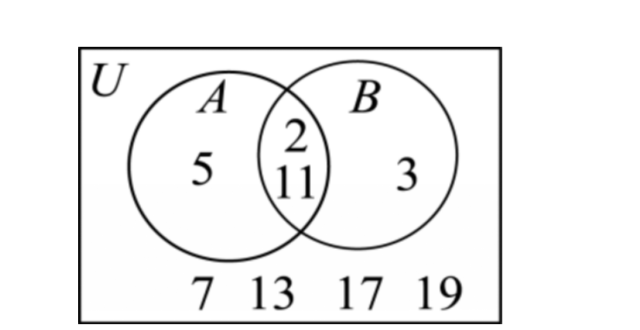
\includegraphics[width=0.24\textwidth]{figures/gao108_q6.png}
\end{center}

\solend
\fi

\item 若 $x\in A$，则 $\dfrac1x\in A$，就称 $A$ 自倒集合，集合 $M=\left\{-2,-1,0,\dfrac12,\dfrac13,1,2,3,4\right\}$ 的所有非空
子集中，自倒集合的个数为\blankline[4.4em].

\ifanswer
\solbegin
\step{由新定义，集合 $M$ 中的元素 1 和 $-1$ 倒数等于本身，2 和 $\dfrac12$，3 和 $\dfrac13$ 互为倒数,}
\step{故满足条件的自倒集合与集合 $\{-1,1,2,3\}$ 的非空子集的个数相同,}
\step{则其个数为 $2^4-1=15$.}
\solend
\fi

\item 设集合 $M=\{(x,y)\mid y=x^2+2bx+1\}$，$N=\{(x,y)\mid y=x+b\}(b\in\R)$，若
$M\cap N=\varnothing$，则实数 $b$ 的取值范围为\blankline[4.4em].

\ifanswer
\solbegin
\step{因为 $M\cap N=\varnothing$，所以
$\begin{cases}y=x^2+2bx+1\\y=x+b\end{cases}$
无解，则 $x^2+(2b-1)x+(1-b)=0$,}
\step{则 $\triangle=(2b-1)^2-4\times1\times(1-b)=4b^2-3<0$，解得 $-\dfrac{\sqrt3}2<b<\dfrac{\sqrt3}2$,}
\step{即实数 $b$ 的取值范围为 $\left(-\dfrac{\sqrt3}2,\dfrac{\sqrt3}2\right)$.}
\solend
\fi

\item 已知集合 $A=\left\{x\,\middle|\,\dfrac{x-a}{x^2-1}=1\right\}$ 有唯一元素，用列举法表示满足集合 $A$ 的条件的 $a$ 的取值集
合\blankline[4.4em].

\ifanswer
\solbegin
\step{$a=1$,$\dfrac{1}{x+1}=1$，一解；$a=-1$,$\dfrac{1}{x-1}=1$，一解；}
\step{$x-a=x^2-1$，一解时，$a=\dfrac54$,}
\step{综上，$a$ 的取值集合为 $\left\{-1,1,\dfrac54\right\}$.}
\solend
\fi

\item 已知集合 $M$ 的元素均为正整数，定义集合 $M$ 的“变项和”为：将 $M$ 中每个元素 $m$ 都乘
以 $(-1)^n$ 后再求和. 若集合 $A=\{n\mid1\leqslant n\leqslant2026,n\in\N\}$，则集合 $A$ 的所有非空子集的“变
项和”的总和为\blankline[4.4em].% $n$ 未加界定（据解析为元素序号），照录

\ifanswer
\solbegin
\step{$A=\{n\mid1\leqslant n\leqslant2026,n\in\N\}=\{1,2,\cdots,2026\}$,}
\step{1 在所有非空子集中共出现 $C_{2025}^{0}+C_{2025}^{1}+\cdots+C_{2025}^{2025}=2^{2025}$ 次,}
\step{同理 $2,3,\cdots,2026$ 都出现 $2^{2025}$ 次,}
\step{则集合 $A$ 的所有非空子集的“变项和”的总和}
\step{为 $2^{2025}\times[1\times(-1)^1+2\times(-1)^2+\cdots+2026\times(-1)^{2026}]$}
\step{$=2^{2025}\times(-1+2-3+4-\cdots-2025+2026)=1013\times2^{2025}$.}
\solend
\fi

\item 已知 $0<k<2$，定义 $[x]$ 为不超过 $x$ 的最大整数，区间 $[a,b]$（或 $(a,b)$，$[a,b)$，
$(a,b]$）的长度记为 $b-a$. 若关于 $x$ 的不等式 $k[x]>\lvert2[x]-6\rvert$ 的解集对应区间的长度为 $2$，
则 $k$ 的取值范围是\blankline[4.4em].

\ifanswer
\solbegin
\stepm{法一：}{由题意得 $\lvert2[x]-6\rvert=
\begin{cases}2[x]-6,x\geqslant3\\-2[x]+6,x<3\end{cases}$.}
\step{①当 $x\geqslant3$ 时，不等式 $k[x]>\lvert2[x]-6\rvert$ 可化为 $k[x]>2[x]-6$,}
\step{即 $(2-k)[x]<6$,}
\step{当 $0<k<2$ 时，解不等式 $(2-k)[x]<6$ 得 $[x]<\dfrac6{2-k}$.}
\step{②当 $x<3$ 时，不等式 $k[x]>\lvert2[x]-6\rvert$ 可化为 $k[x]>-2[x]+6$,}
\step{即 $(k+2)[x]>6$.}
\step{当 $0<k<2$ 时，解不等式 $(k+2)[x]>6$ 得 $[x]>\dfrac6{k+2}$.}
\step{综上所述，不等式 $k[x]>\lvert2[x]-6\rvert$ 的解集需满足 $\dfrac6{k+2}<[x]<\dfrac6{2-k}$,}
\step{由题意得在区间 $\left[\dfrac6{k+2},\dfrac6{2-k}\right]$ 内有两个整数,}
\step{由于 $\dfrac6{k+2}\in\left(\dfrac32,3\right)$，所以 $\dfrac6{2-k}\leqslant5$，得 $k\leqslant\dfrac45$.}
\step{因此 $k\in\left(0,\dfrac45\right]$，得 $\dfrac6{k+2}\in\left[\dfrac75,3\right)$，$\dfrac6{2-k}\in(3,5]$,}
\step{区间 $\left[\dfrac6{k+2},\dfrac6{2-k}\right]$ 内的两个整数是 3、4，所以 $4<\dfrac6{2-k}\leqslant5$，解得 $\dfrac12<k\leqslant\dfrac45$,}
\step{即 $k\in\left(\dfrac12,\dfrac45\right]$.}
\stepm{法二：}{令 $f(x)=kx$，$g(x)=\lvert2x-6\rvert$，画出 $g(x)$、$f(x)$ 的图象,}
\step{由于不等式 $k[x]>\lvert2[x]-6\rvert$ 的解集对应区间的长度为 2,}
\step{因此解集只可能为 $[3,5)$ 或 $[2,4)$.}
\step{当解集为 $[3,5)$ 时，如图（2），数形结合易得
$\begin{cases}f(2)\leqslant g(2)\\f(4)>g(4)\\f(5)\leqslant g(5)\end{cases}$,}
\step{即
$\begin{cases}2k\leqslant\lvert2\times2-6\rvert\\4k>\lvert2\times4-6\rvert\\5k\leqslant\lvert2\times5-6\rvert\end{cases}$，
解得
$\begin{cases}k\leqslant1\\k>\dfrac12\\k\leqslant\dfrac45\end{cases}$，
所以 $\dfrac12<k\leqslant\dfrac45$，满足 $0<k<2$,}
\step{当解集为 $[2,4)$ 时，如图（1），数形结合易得
$\begin{cases}f(2)>g(2)\\f(4)\leqslant g(4)\end{cases}$,}
\step{即
$\begin{cases}2k>\lvert2\times2-6\rvert\\4k\leqslant\lvert2\times4-6\rvert\end{cases}$，
无解.}

\begin{center}
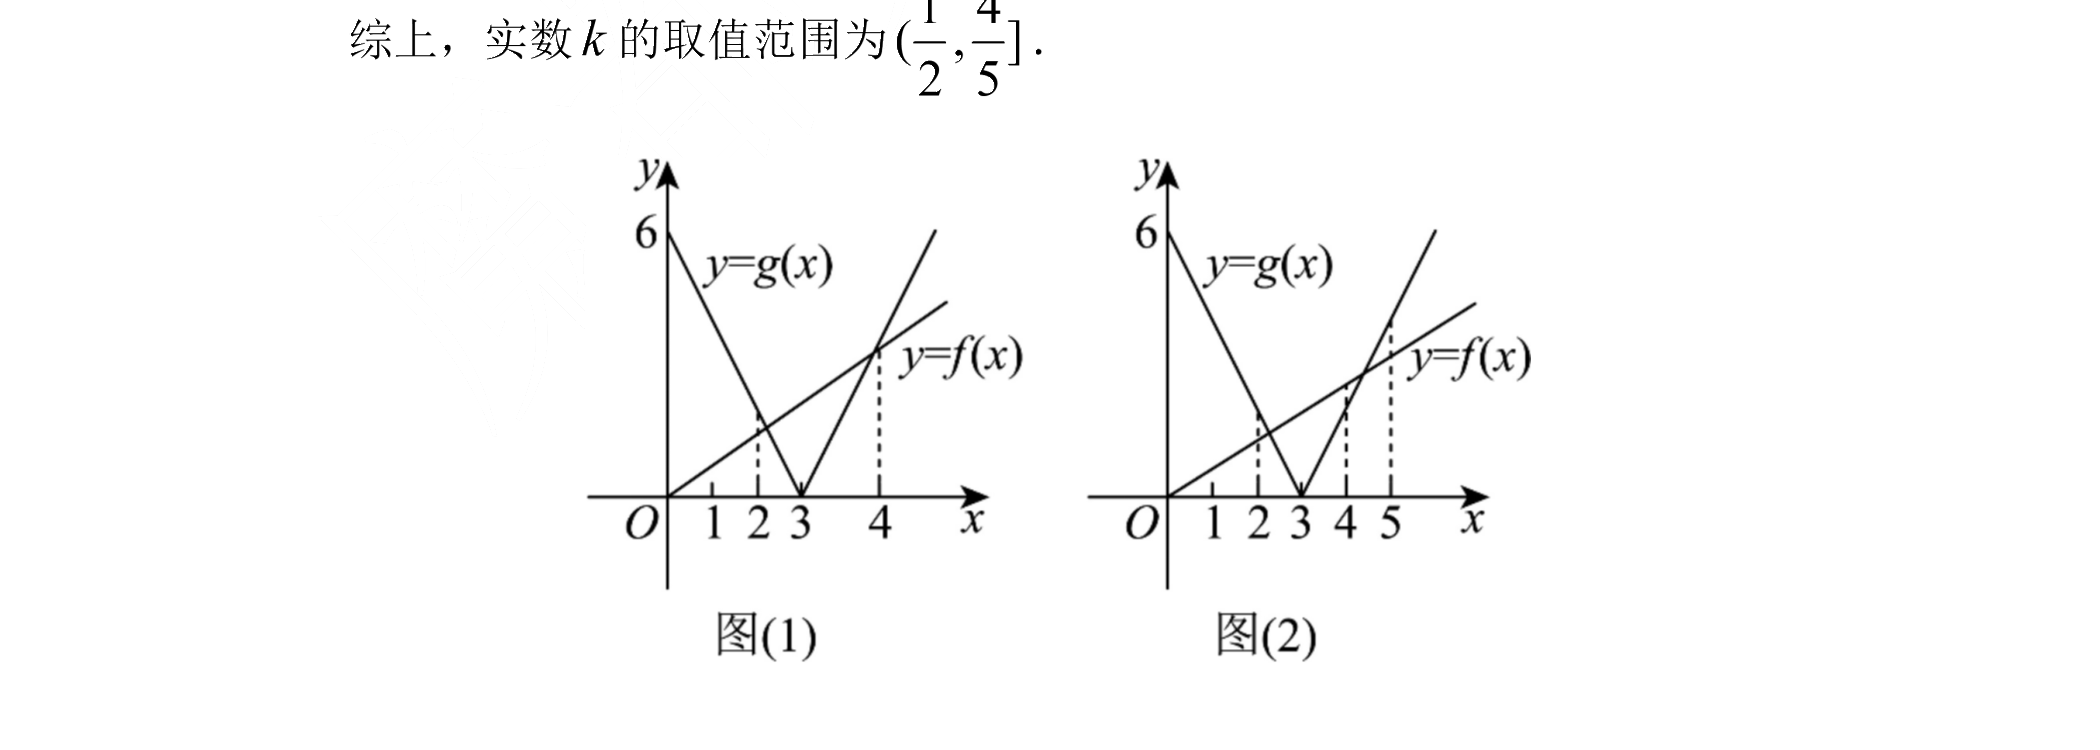
\includegraphics[width=0.72\textwidth]{figures/gao108_q11.png}
\end{center}

\step{综上，实数 $k$ 的取值范围为 $\left(\dfrac12,\dfrac45\right]$.}
\solend
\fi

\item 已知集合 $A=[1,a]\cup[a^3,a^4]$，集合 $B=\{x\mid x=x_1-x_2$，其中 $x_1$,$x_2\in A\}$. 若集合 $B$ 表
示的区间为一个闭区间，则实数 $a$ 的取值范围为\blankline[4.4em].

\ifanswer
\solbegin
\step{由题意得 $a^3>a>1$，则 $x_1-x_2$ 的最小值为 $1-a^4$，最大值为 $a^4-1$,}
\step{所以 $B=[1-a^4,a^4-1]$,}
\step{又因为 $a^4-a^3-(a-1)=a^3(a-1)-(a-1)=(a^3-1)(a-1)>0$,}
\step{所以 $a^4-a^3>a-1$，又集合 $B$ 表示的区间为一个闭区间,}
\step{则 $a^3-a\leqslant a^4-a^3$，化简得 $a^2-a-1\geqslant0$，又 $a>1$，解得 $a\geqslant\dfrac{1+\sqrt5}2$.}
\solend
\fi

\end{enumerate}

\bigsec{二、选择题}

\begin{enumerate}
\setcounter{enumi}{12}

\item 若 $a,b,c\in\R$，则下列不等式恒成立的是\mbox{（\quad）}% 原卷把答案“C”印在题干括号内、无【解析】

\keepwithprev
A. $\dfrac1a<\dfrac1b$\qquad B. $a^2<b^2$\qquad C. $\dfrac{a}{c^2+1}>\dfrac{b}{c^2+1}$\qquad D. $a\lvert c\rvert>b\lvert c\rvert$

\ifanswer
\ans{$C$}
\fi

\item 以下几个关系中正确的是\mbox{（\quad）}

\keepwithprev
A. $0\in\varnothing$\qquad\qquad\qquad B. $\varnothing\in\{x\mid x^2+1=0\}$

C. $\varnothing\subset\{0\}$\qquad\qquad\qquad D. $(A\cap B)\subset(A\cup B)$

\ifanswer
\solbegin
\step{$A$ 选项，$\varnothing$ 不包含任何元素，所以 $0\in\varnothing$ 错误，$A$ 错,}
\step{$B$ 选项，集合与集合之间关系不可以用 $\in$，$B$ 错,}
\step{$C$ 选项，空集是非空集合的真子集，所以 $\varnothing\subset\{0\}$ 正确，$C$ 对,}
\step{$D$ 选项，当 $A=B$ 时，$(A\cap B)=(A\cup B)$，$D$ 错,}
\step{故选 $C$.}
\solend
\fi

\item 设全集为 $U$，图中阴影部分所表示的集合是\mbox{（\quad）}% 原卷把答案“A”印在题干括号内、无【解析】

\keepwithprev
A. $B\cap\overline{A\cup C}$\qquad\qquad B. $(A\cup B)\cap(B\cup C)$

C. $(A\cup C)\cap\overline B$\qquad\qquad D. $(\overline A\cup\overline C)\cap B$

\ifanswer
\ans{$A$}
\fi

\item 对于 $k=0,1,2,\cdots$，定义集合 $A_k=\{20+k,26+2k\}$，并记 $S_k=A_0\cup A_1\cup\cdots\cup A_k$，则
使得集合 $S_n$ 中完全平方数的个数为奇数的最小正整数 $n$ 为\mbox{（\quad）}

\keepwithprev
A. $18$\qquad\qquad B. $19$\qquad\qquad C. $20$\qquad\qquad D. $21$

\ifanswer
\solbegin
\step{当 $k=0$ 时，$A_0=\{20,26\}$，对于 $k=0,1,2,\cdots$,}
\step{集合 $A_k$ 中最小的元素 $20>4^2$，若 $S_n$ 中完全平方数的个数为奇数，则 $n>4$,}
\step{（1）$20+k=5^2$ 时，$k=5$，$A_5=\{25,36\}$，此时 $S_5$ 中完全平方数为 $5^2$、$6^2$,}
\step{个数为 2;}
\step{$20+k=6^2$ 时，$k=16$，$A_{16}=\{36,58\}$，此时 $S_{16}$ 中完全平方数为 $5^2$、$6^2$,}
\step{个数为 2;}
\step{$20+k=7^2$ 时，$k=29$，$A_{29}=\{49,84\}$,}
\step{此时 $S_{29}$ 中完全平方数为 $5^2$、$6^2$、$7^2$、$8^2$，个数为 4;}
\step{$20+k=8^2$ 时，$k=44$，$A_{44}=\{64,114\}$,}
\step{此时 $S_{44}$ 中完全平方数为 $5^2$、$6^2$、$7^2$、$8^2$、$10^2$，个数为 5;}
\step{（2）因为 $k=0,1,2,\cdots,26+2k$ 一定为偶数,}
\step{所以 $26+2k=6^2$ 时，$k=5$，由上述分析得 $S_5$ 中完全平方数个数为 2;}
\step{$26+2k=8^2$ 时，$k=19$，$A_{19}=\{39,64\}$,}
\step{此时 $S_{19}$ 中完全平方数为 $5^2$、$6^2$、$8^2$，个数为 3.}
\step{综上，使集合 $S_n$ 中完全平方数的个数为奇数的最小正整数 $n=19$. 故选 $B$.}
\solend
\fi

\end{enumerate}

\bigsec{三、解答题}

\begin{enumerate}
\setcounter{enumi}{16}

\item 设全集 $U=\R$，集合 $A=\left\{x\,\middle|\,\dfrac{x-2}{x+2}\leqslant0\right\}$，$B=\{x\mid a\leqslant x<2a+1,a\in\R\}$，
$C=\{x\mid\lvert2x-1\rvert<5\}$.

（1）求集合 $A$、$\overline A\cup C$；

（2）若 $B\subseteq A$，求实数 $a$ 的取值范围.

\ifanswer
\solbegin
\ansspace*
\step{（1）不等式 $\dfrac{x-2}{x+2}\leqslant0$，等价于
$\begin{cases}(x-2)(x+2)\leqslant0\\x+2\neq0\end{cases}$，
解得 $\{x\mid-2<x\leqslant2\}$,}
\step{所以 $A=\{x\mid-2<x\leqslant2\}$，则 $\overline A=\{x\mid x\leqslant-2$ 或 $x>2\}$,}
\step{因为 $C=\{x\mid\lvert2x-1\rvert<5\}=\{x\mid-2<x<3\}$，所以 $\overline A\cup C=\R$；}
\step{（2）因为 $B\subseteq A$,}
\step{若 $B=\varnothing$，则 $a\geqslant2a+1$，解得 $a\leqslant-1$,}
\step{若 $B\neq\varnothing$，则
$\begin{cases}a<2a+1\\a>-2\\2a+1\leqslant2\end{cases}$，
解得 $-1<a\leqslant\dfrac12$,}
\step{综上所述，实数 $a$ 的取值范围为 $\left\{a\,\middle|\,a\leqslant\dfrac12\right\}$.}
\solend
\fi

\item 设 $a$、$b$、$c$、$d$ 是四个正数.

（1）已知 $a>b$，比较 $\dfrac{2a+b}{a+2b}$ 与 $\dfrac ab$ 的值的大小；

（2）若 $(1+a)(1+b)(1+c)(1+d)<16$，求证：$a$、$b$、$c$、$d$ 中至少有一个小于 1.

\ifanswer
\solbegin
\step{（1）$\dfrac{2a+b}{a+2b}-\dfrac ab=\dfrac{b^2-a^2}{b(a+2b)}<0$，所以 $\dfrac{2a+b}{a+2b}<\dfrac ab$.}
\step{（2）假设 $a$、$b$、$c$、$d$ 都不小于 1，即 $a$、$b$、$c$、$d$ 均大于等于 1,}
\step{即 $a\geqslant1$，$b\geqslant1$，$c\geqslant1$，$d\geqslant1$,}
\step{由均值不等式得 $1+a\geqslant2\sqrt a$,$1+b\geqslant2\sqrt b$,$1+c\geqslant2\sqrt c$,$1+d\geqslant2\sqrt d$,}
\step{故 $(1+a)(1+b)(1+c)(1+d)\geqslant16\sqrt{abcd}\geqslant16$,}
\step{当且仅当 $a=b=c=d=1$ 时取等号,}
\step{这与 $(1+a)(1+b)(1+c)(1+d)<16$ 矛盾，故假设不成立，原命题成立.}
\solend
\fi

\item 已知 $m\in\R$，一个二次项系数为 1 的一元二次方程的两个不等实根分别为 $x_1$ 和 $x_2$，且
满足
$\begin{cases}x_1^2+x_2^2=2m^2-4\\x_1+x_2=m\end{cases}$.

（1）直接写出该一元二次方程；

（2）若 $(3x_1-x_2)(3x_2-x_1)\geqslant-1$，求 $m$ 的取值范围；

（3）若方程的两根 $x_1$ 和 $x_2$ 都大于 $-1$，求 $m$ 的取值范围.

\ifanswer
\solbegin
\step{（1）设这个一元二次方程为 $x^2+bx+c=0$,}
\step{由
$\begin{cases}x_1^2+x_2^2=2m^2-4\\x_1+x_2=m\end{cases}$,}
\step{得 $(x_1+x_2)^2=x_1^2+x_2^2+2x_1x_2=2m^2-4+2x_1x_2=m^2$，即 $x_1x_2=\dfrac{4-m^2}2$,}
\step{由韦达定理得 $x_1+x_2=-b=m$，即 $x_1x_2=c=\dfrac{4-m^2}2$,}
\step{所以一元二次方程为 $x^2-mx+\dfrac{4-m^2}2=0$.}
\step{（2）$(3x_1-x_2)(3x_2-x_1)=9x_1x_2-3x_1^2-3x_2^2+x_1x_2=10x_1x_2-3(x_1^2+x_2^2)\geqslant-1$,}
\step{结合已知及（1）得 $x_1^2+x_2^2=2m^2-4$,$x_1x_2=\dfrac{4-m^2}2$,}
\step{代入得 $10\times\dfrac{4-m^2}2-3(2m^2-4)=-11m^2+32\geqslant-1\Rightarrow m^2\leqslant3$}
\step{$\Rightarrow-\sqrt3\leqslant m\leqslant\sqrt3$,}
\step{又 $\Delta=m^2-4\times\dfrac{4-m^2}2=3m^2-8>0\Rightarrow m<-\dfrac{2\sqrt6}3$ 或 $m>\dfrac{2\sqrt6}3$,}
\step{所以 $m\in\left[-\sqrt3,-\dfrac{2\sqrt6}3\right)\cup\left(\dfrac{2\sqrt6}3,\sqrt3\right]$.}
\step{（3）若方程的两根 $x_1$ 和 $x_2$ 都大于 $-1$，则
$\begin{cases}\Delta>0\\x_1+x_2>-2\\(x_1+1)(x_2+1)>0\end{cases}$,}
\step{所以
$\begin{cases}\Delta=3m^2-8>0\\m>-2\\[2pt]\dfrac{4-m^2}2+m+1>0\end{cases}$，
解得 $m\in\left(1-\sqrt7,-\dfrac{2\sqrt6}3\right)\cup\left(\dfrac{2\sqrt6}3,1+\sqrt7\right)$.}
\solend
\fi

\item 已知不等式 $2\leqslant ax^2+bx+c\leqslant3$ 的解集为 $\{x\mid2\leqslant x\leqslant3\}$.

（1）若 $a>0$，求 $6b+5c$ 的值；

（2）若 $a>0$，且不等式 $ax^2+(b-3)x-c\leqslant0$ 有且仅有 9 个整数解，求 $a$ 的取值范围；

（3）若 $a<0$，对任意的 $x<0$，不等式 $(ax-4)(x^2+b+c+1)\geqslant0$ 恒成立，求 $a^2-b+c$
的取值集合.

\ifanswer
\solbegin
\ansspace*
\step{（1）$a>0$,}
\step{结合二次函数图象得不等式 $ax^2+bx+c\leqslant3$ 的解集为 $\{x\mid2\leqslant x\leqslant3\}$,}
\step{且不等式 $ax^2+bx+c\geqslant2$ 的解集为 $R$,}
\step{所以方程 $ax^2+bx+c-3=0$ 的两根分别为 2 和 3,}
\step{则
$\begin{cases}2+3=-\dfrac ba\\[2pt]2\times3=\dfrac{c-3}a\end{cases}$，
得 $b=-5a$，$c=6a+3$,}
\step{所以 $6b+5c=6\times(-5a)+5(6a+3)=15$.}
\step{（2）若 $a>0$，且不等式 $ax^2+(b-3)x-c\leqslant0$ 有且仅有 9 个整数解,}
\step{由（1）得 $b=-5a$，$c=6a+3$,}
\step{不等式 $ax^2+bx+c\geqslant2$ 可化为 $ax^2-5ax+6a+1\geqslant0$.}
\step{由（1）得不等式 $ax^2+bx+c\geqslant2$ 的解集为 $R$,}
\step{所以 $ax^2-5ax+6a+1\geqslant0$ 恒成立,}
\step{所以
$\begin{cases}a>0\\\Delta=25a^2-4a(6a+1)\leqslant0\end{cases}$，
即
$\begin{cases}a>0\\a^2-4a=a(a-4)\leqslant0\end{cases}$，}
\step{解得 $0<a\leqslant4$.}
\step{不等式 $ax^2+(b-3)x-c\leqslant0$ 等价于 $ax^2-(5a+3)x-(6a+3)\leqslant0$,}
\step{所以 $[ax-(6a+3)](x+1)\leqslant0$，得 $-1\leqslant x\leqslant6+\dfrac3a$,}
\step{所以 $7\leqslant6+\dfrac3a<8$，解得 $\dfrac32<a\leqslant3$.}
\step{综上，$a$ 的取值范围为 $\left(\dfrac32,3\right]$.}
\step{（3）因为 $a<0$,}
\step{同（1）分析，不等式 $ax^2+bx+c\geqslant2$ 的解集为 $\{x\mid2\leqslant x\leqslant3\}$,}
\step{$ax^2+bx+c\leqslant3$ 的解集为 $R$,}
\step{所以方程 $ax^2+bx+c-2=0$ 的两根分别为 2 和 3,}
\step{则
$\begin{cases}2+3=-\dfrac ba\\[2pt]2\times3=\dfrac{c-2}a\end{cases}$，
得 $b=-5a$，$c=6a+2$.}
\step{所以不等式 $ax^2+bx+c=ax^2-5ax+6a+2\leqslant3$ 的解集为 $R$,}
\step{则 $ax^2-5ax+6a-1\leqslant0$ 恒成立,}
\step{所以
$\begin{cases}a<0\\\Delta=25a^2-4a(6a-1)\leqslant0\end{cases}$，
即
$\begin{cases}a<0\\a^2+4a=a(a+4)\leqslant0\end{cases}$，}
\step{解得 $-4\leqslant a<0$.}
\step{所以对任意的 $x<0$，不等式 $(ax-4)(x^2+b+c+1)\geqslant0$ 恒成立}
\step{转化为对任意的 $x<0$，不等式 $(ax-4)(x^2+a+3)\geqslant0$ 恒成立.}
\step{方程 $(ax-4)(x^2+a+3)=0$ 的两个根为 $x=\dfrac4a<0$,}
\step{$x=\pm\sqrt{-a-3}$（$a<-3$ 时成立）,}
\step{因而仅当 $ax-4=0$ 与 $x^2+a+3=0$ 的负根重合时满足条件,}
\step{解得唯一解为 $a=-4$，所以 $a^2-b+c=a^2+11a+2=-26$,}
\step{所以 $a^2-b+c$ 的取值集合为 $\{-26\}$.}
\solend
\fi

\item 已知集合 $A=\{1,2,3,4,5,6,7,8\}$，$M=\{(x,y)\mid x\in A,y\in A\}$，从 $M$ 中选取 $n$ 个不同的
元素组成一个序列：$(x_1,y_1)$,$(x_2,y_2),\cdots,(x_n,y_n)$，其中 $(x_i,y_i)$ 称为该序列的第 $i$ 项
（$i=1,2,\cdots,n$），若该序列的相邻项 $(x_i,y_i)$,$(x_{i+1},y_{i+1})$ 满足：
\[\begin{cases}\lvert x_{i+1}-x_i\rvert=3\\\lvert y_{i+1}-y_i\rvert=4\end{cases}
\quad\text{或}\quad
\begin{cases}\lvert x_{i+1}-x_i\rvert=4\\\lvert y_{i+1}-y_i\rvert=3\end{cases}\]
（$i=1,2,\cdots,n-1$），则称该序列为“$\Delta-$序列”.

（1）若一个 $\Delta-$序列的第一项为 $(4,4)$，请直接写出它所有可能的第二项；

（2）定义集合 $A=\{1,2,3,4,5,6,7,8\}$ 的两个子集：外侧集 $S=\{1,2,7,8\}$，内侧集
$T=\{3,4,5,6\}$. 证明：若 $\Delta-$序列中某一项的坐标在区域 $S\times S$ 内（即横、纵坐标均属于
$S$），则它的下一项坐标必定在区域 $T\times T$ 内；

（3）证明：不存在一个恰好有 5 项的 $\Delta-$序列，使其第一项为 $(1,8)$，且第五项为
$(8,1)$.

\ifanswer
\solbegin
\ansspace*
\step{（1）由题意，第一项为 $(x_1,y_1)=(4,4)$,}
\step{对于第二项 $(x_2,y_2)$，其坐标必须在 1~8 之间.}
\step{若 $\lvert x_2-4\rvert=3$,$\lvert y_2-4\rvert=4$，则 $x_2\in\{1,7\}$,}
\step{且 $y_2\in\{8\}$（因为 $4-4=0$ 不在集合 $A$ 中）. 此时可能的点为 $(1,8)$,$(7,8)$.}
\step{若 $\lvert x_2-4\rvert=4$,$\lvert y_2-4\rvert=3$，则 $x_2\in\{8\}$，且 $y_2\in\{1,7\}$.}
\step{此时可能的点为 $(8,1)$,$(8,7)$.}
\step{所以它所有可能的第二项为 $(1,8)$,$(7,8)$,$(8,1)$,$(8,7)$.}
\step{（2）已知某一项 $(x_t,y_t)\in S\times S$，即 $x_t\in\{1,2,7,8\}$ 且 $y_t\in\{1,2,7,8\}$.}
\step{由规则得下一步坐标的变化量为 3 和 4，设 $a\in S$ 变化 3 或 4 后的结果 $a'$:}
\step{当 $a=1$ 时，$1+3=4\in T$,$1+4=5\in T$；}
\step{当 $a=2$ 时，$2+3=5\in T$,$2+4=6\in T$；}
\step{当 $a=7$ 时，$7-3=4\in T$,$7-4=3\in T$；}
\step{当 $a=8$ 时，$8-3=5\in T$,$8-4=4\in T$.}
\step{（注：由于超出 1~8 范围的越界坐标不符合.）}
\step{由此可见，无论 $a$ 是 $S$ 中的哪一个数，加上或减去 3 或 4 之后,}
\step{得到的新坐标必属于集合 $T$.}
\step{因为 $\Delta-$序列每走一步，横坐标和纵坐标必定同时发生 3 和 4 的变化,}
\step{所以新的横坐标 $x_{i+1}$ 必属于 $T$，新的纵坐标 $y_{i+1}$ 也必属于 $T$,}
\step{即下一项 $(x_{i+1},y_{i+1})$ 必定在区域 $T\times T$ 内. ………10 分原命题得证.% 得分行混入证明，照录
}
\step{（3）假设存在这样一个包含 5 项的 $\Delta-$序列:}
\step{$(x_1,y_1)$,$(x_2,y_2)$,$(x_3,y_3)$,$(x_4,y_4)$,$(x_5,y_5)$.}
\step{已知第一项为 $(1,8)$，第五项为 $(8,1)$. 第 2 项必须是第 1 项 $(1,8)$ 的相邻点.}
\step{我们来找 $(1,8)$ 的相邻点：第 2 项只能是 $(4,4)$ 或 $(5,5)$,}
\step{第 4 项必须是第 5 项 $(8,1)$ 的相邻点（因为跳跃是双向可逆的）.}
\step{同理可算得，$(8,1)$ 的相邻点也只有两个：$(4,4)$ 和 $(5,5)$,}
\step{题目题干中明确规定，$\Delta-$序列由 $n$ 个不同的有序数对构成.% “题目题干”措辞重复，照录
}
\step{所以，第 2 项和第 4 项不能是同一个点. 这就意味着:}
\step{如果第 2 项是 $(4,4)$，第 4 项就必须是 $(5,5)$；反之亦然.}
\step{则第 3 项必须是 $(4,4)$ 和 $(5,5)$ 的公共相邻点.}
\step{$(4,4)$ 的相邻点集合为：$\{(1,8),(7,8),(8,1),(8,7)\}$,}
\step{$(5,5)$ 的相邻点集合为：$\{(2,1),(8,1),(1,2),(1,8)\}$,}
\step{所以，第 3 项只能填 $(1,8)$ 或者 $(8,1)$.}
\step{这与“序列由不同的有序数对构成”这一条件产生矛盾！}
\step{所以，不存在一个恰好有 5 项的 $\Delta-$序列,}
\step{使其第一项为 $(1,8)$，且第五项为 $(8,1)$.}
\solend
\fi

\end{enumerate}

\end{document}
"
% 紧凑版：xelatex "\def\iscompact{1}% 高一108_五校联考_10月月考.tex
%   —— 高一上数学“2026-2027 年五校联考高一上 10 月月考”（试卷版/答案版）
% 试卷版：xelatex 高一108_五校联考_10月月考.tex
% 答案版：xelatex "\def\isanswer{1}\input{高一108_五校联考_10月月考.tex}"
% 紧凑版：xelatex "\def\iscompact{1}\input{高一108_五校联考_10月月考.tex}"
%
% 原始材料：微信公众号“魔都数学加油站”文章，作者破晓，2026-11-03 17:19 发布；
% 连载“27学年高一108”，原文标题“27学年高一108——2026-2027年上海市五校联考高一上10月月考”；
% 原文链接：https://mp.weixin.qq.com/s/3nkP789Qar93NGMZXFFCSw。
% 正文为 14 张 PNG 页（第 2、3、6—13 页 4762×6735，第 1、4、5、14 页 2560×3620），
% 题目下印有【解析】，为讲评版。
% 题目、解析均据原图转录；卷面水印及公众号页脚未录入。
% 第 6 题解析的文氏图与第 11 题法二解析的两幅图象（图(1)、图(2)）裁自原图、去粉色水印
% 转灰度（gao108_q6.png、gao108_q11.png），第 6 题图属解析（仅答案版）、
% 第 11 题图属解析（仅答案版）。
%
% 卷首标题：原卷印作“2026-2027 年五校联考高一上 10 月月考”，标题下另印一行参与学校
% 名单“闵行中学、嘉定一中、松江一中、金山中学、嘉一实高”（全稿第 5 份原卷自印副标题，
% 按 14／24／49／50 成例照录，并登记进计数核对.py 的 SELFSUB）。
%
% 与原卷的排版差异：
%   ① 原文从第 3 题起，填空题编号为 3—12、选择题为 13—16、解答题为 17—21，本稿保留原题号；
%   ② 原卷每题下直接印【解析】，本稿按全稿惯例将解析置于答案版；第 4 题只印【答案】，
%      第 13、15 两题把答案印在题干括号内且无【解析】，均另提 \ans{}；
%   ③ 原卷副标题照录（见上）；
%   ④ 原卷填空横线按全稿惯例排为 \blankline[4.4em]；解答题按惯例加 \ansspace；选择题括号排
%      \mbox{（\quad）}、选项段前按惯例加 \keepwithprev；
%   ⑤ 原卷数集排斜体 $R$／$N$，按全稿惯例改 \R、\N。
%
% 原卷红色强调照录为黑体：第 11 题解析的“法一：”“法二：”原卷排红色，按 53 成例排
% \stepm{法一：}／\stepm{法二：}（加粗着色）。
%
% 原卷存疑：第 10 题题干“变项和”定义中“将 $M$ 中每个元素 $m$ 都乘以 $(-1)^n$ 后再求和”
% 的 $n$ 未加界定（据解析应为该元素在 $\{1,2,\cdots,2026\}$ 中的序号），照录。
% 第 21 题 (2) 解析末行“即下一项 $(x_{i+1},y_{i+1})$ 必定在区域 $T\times T$ 内. ………10 分
% 原命题得证.”，原卷把得分点行混入证明（“原命题”按上下文为“原命题的逆否”），照录。
% 第 21 题 (3) 解析“题目题干中明确规定”，“题目题干”措辞重复，照录。
%
% 行数核对：逐题数 \step/\stepm 条数，合计 164 条（Q3：3；Q4：0；Q5：2；Q6：1；Q7：3；
% Q8：3；Q9：3；Q10：6；Q11：21；Q12：5；Q13：0；Q14：5；Q15：0；Q16：15；Q17：7；
% Q18：7；Q19：13；Q20：34；Q21：36），与原卷印刷行逐题相等。第 4 题只印【答案】、
% 第 13、15 题括号内印答案，均提 \ans{}，不计入 \step 账。
%
\documentclass[a4paper,11pt]{article}
\usepackage{common}

\begin{document}

\examtitlest[3]{2026--2027 年五校联考高一上 10 月月考}{闵行中学、嘉定一中、松江一中、金山中学、嘉一实高}

\bigsec{一、填空题}

\begin{enumerate}
\setcounter{enumi}{2}

\item 已知等式 $2x^2+3x+5=2ax^2+a(3x+1)+c$ 恒成立，则实数 $a+c$ 的值为\blankline[4.4em].

\ifanswer
\solbegin
\step{因为 $2x^2+3x+5=2ax^2+a(3x+1)+c$ 恒成立,}
\step{即 $2x^2+3x+5=2ax^2+3ax+(a+c)$ 恒成立，所以
$\begin{cases}2=2a\\3=3a\\5=a+c\end{cases}$,}
\step{所以 $a+c=5$.}
\solend
\fi

\item 不等式 $\dfrac1x<\dfrac12$ 的解集是\blankline[4.4em].

\ifanswer
\ans{$(-\infty,0)\cup(2,+\infty)$}
\fi

\item 已知 $a$、$b$ 都是实数，则“$a^2=b^2$”是“$a^2+b^2=2ab$”的\blankline[4.4em]条件.

\ifanswer
\solbegin
\step{$a^2=b^2$ 等价于 $a=\pm b$；$a^2+b^2=2ab$ 等价于 $(a-b)^2=0$ 等价于 $a=b$,}
\step{故“$a^2=b^2$”是“$a^2+b^2=2ab$”的必要不充分条件.}
\solend
\fi

\item 已知全集 $U=\{x\mid x$ 为不大于 20 的素数$\}$，$A\cap\overline B=\{5\}$，$\overline A\cap B=\{3\}$，
$\overline{A\cup B}=\{7,13,17,19\}$，则 $A=$\blankline[4.4em].

\ifanswer
\solbegin
\step{如图所示，$A=\{2,5,11\}$.}

\begin{center}
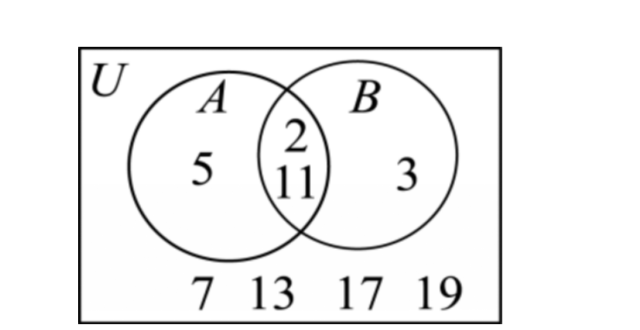
\includegraphics[width=0.24\textwidth]{figures/gao108_q6.png}
\end{center}

\solend
\fi

\item 若 $x\in A$，则 $\dfrac1x\in A$，就称 $A$ 自倒集合，集合 $M=\left\{-2,-1,0,\dfrac12,\dfrac13,1,2,3,4\right\}$ 的所有非空
子集中，自倒集合的个数为\blankline[4.4em].

\ifanswer
\solbegin
\step{由新定义，集合 $M$ 中的元素 1 和 $-1$ 倒数等于本身，2 和 $\dfrac12$，3 和 $\dfrac13$ 互为倒数,}
\step{故满足条件的自倒集合与集合 $\{-1,1,2,3\}$ 的非空子集的个数相同,}
\step{则其个数为 $2^4-1=15$.}
\solend
\fi

\item 设集合 $M=\{(x,y)\mid y=x^2+2bx+1\}$，$N=\{(x,y)\mid y=x+b\}(b\in\R)$，若
$M\cap N=\varnothing$，则实数 $b$ 的取值范围为\blankline[4.4em].

\ifanswer
\solbegin
\step{因为 $M\cap N=\varnothing$，所以
$\begin{cases}y=x^2+2bx+1\\y=x+b\end{cases}$
无解，则 $x^2+(2b-1)x+(1-b)=0$,}
\step{则 $\triangle=(2b-1)^2-4\times1\times(1-b)=4b^2-3<0$，解得 $-\dfrac{\sqrt3}2<b<\dfrac{\sqrt3}2$,}
\step{即实数 $b$ 的取值范围为 $\left(-\dfrac{\sqrt3}2,\dfrac{\sqrt3}2\right)$.}
\solend
\fi

\item 已知集合 $A=\left\{x\,\middle|\,\dfrac{x-a}{x^2-1}=1\right\}$ 有唯一元素，用列举法表示满足集合 $A$ 的条件的 $a$ 的取值集
合\blankline[4.4em].

\ifanswer
\solbegin
\step{$a=1$,$\dfrac{1}{x+1}=1$，一解；$a=-1$,$\dfrac{1}{x-1}=1$，一解；}
\step{$x-a=x^2-1$，一解时，$a=\dfrac54$,}
\step{综上，$a$ 的取值集合为 $\left\{-1,1,\dfrac54\right\}$.}
\solend
\fi

\item 已知集合 $M$ 的元素均为正整数，定义集合 $M$ 的“变项和”为：将 $M$ 中每个元素 $m$ 都乘
以 $(-1)^n$ 后再求和. 若集合 $A=\{n\mid1\leqslant n\leqslant2026,n\in\N\}$，则集合 $A$ 的所有非空子集的“变
项和”的总和为\blankline[4.4em].% $n$ 未加界定（据解析为元素序号），照录

\ifanswer
\solbegin
\step{$A=\{n\mid1\leqslant n\leqslant2026,n\in\N\}=\{1,2,\cdots,2026\}$,}
\step{1 在所有非空子集中共出现 $C_{2025}^{0}+C_{2025}^{1}+\cdots+C_{2025}^{2025}=2^{2025}$ 次,}
\step{同理 $2,3,\cdots,2026$ 都出现 $2^{2025}$ 次,}
\step{则集合 $A$ 的所有非空子集的“变项和”的总和}
\step{为 $2^{2025}\times[1\times(-1)^1+2\times(-1)^2+\cdots+2026\times(-1)^{2026}]$}
\step{$=2^{2025}\times(-1+2-3+4-\cdots-2025+2026)=1013\times2^{2025}$.}
\solend
\fi

\item 已知 $0<k<2$，定义 $[x]$ 为不超过 $x$ 的最大整数，区间 $[a,b]$（或 $(a,b)$，$[a,b)$，
$(a,b]$）的长度记为 $b-a$. 若关于 $x$ 的不等式 $k[x]>\lvert2[x]-6\rvert$ 的解集对应区间的长度为 $2$，
则 $k$ 的取值范围是\blankline[4.4em].

\ifanswer
\solbegin
\stepm{法一：}{由题意得 $\lvert2[x]-6\rvert=
\begin{cases}2[x]-6,x\geqslant3\\-2[x]+6,x<3\end{cases}$.}
\step{①当 $x\geqslant3$ 时，不等式 $k[x]>\lvert2[x]-6\rvert$ 可化为 $k[x]>2[x]-6$,}
\step{即 $(2-k)[x]<6$,}
\step{当 $0<k<2$ 时，解不等式 $(2-k)[x]<6$ 得 $[x]<\dfrac6{2-k}$.}
\step{②当 $x<3$ 时，不等式 $k[x]>\lvert2[x]-6\rvert$ 可化为 $k[x]>-2[x]+6$,}
\step{即 $(k+2)[x]>6$.}
\step{当 $0<k<2$ 时，解不等式 $(k+2)[x]>6$ 得 $[x]>\dfrac6{k+2}$.}
\step{综上所述，不等式 $k[x]>\lvert2[x]-6\rvert$ 的解集需满足 $\dfrac6{k+2}<[x]<\dfrac6{2-k}$,}
\step{由题意得在区间 $\left[\dfrac6{k+2},\dfrac6{2-k}\right]$ 内有两个整数,}
\step{由于 $\dfrac6{k+2}\in\left(\dfrac32,3\right)$，所以 $\dfrac6{2-k}\leqslant5$，得 $k\leqslant\dfrac45$.}
\step{因此 $k\in\left(0,\dfrac45\right]$，得 $\dfrac6{k+2}\in\left[\dfrac75,3\right)$，$\dfrac6{2-k}\in(3,5]$,}
\step{区间 $\left[\dfrac6{k+2},\dfrac6{2-k}\right]$ 内的两个整数是 3、4，所以 $4<\dfrac6{2-k}\leqslant5$，解得 $\dfrac12<k\leqslant\dfrac45$,}
\step{即 $k\in\left(\dfrac12,\dfrac45\right]$.}
\stepm{法二：}{令 $f(x)=kx$，$g(x)=\lvert2x-6\rvert$，画出 $g(x)$、$f(x)$ 的图象,}
\step{由于不等式 $k[x]>\lvert2[x]-6\rvert$ 的解集对应区间的长度为 2,}
\step{因此解集只可能为 $[3,5)$ 或 $[2,4)$.}
\step{当解集为 $[3,5)$ 时，如图（2），数形结合易得
$\begin{cases}f(2)\leqslant g(2)\\f(4)>g(4)\\f(5)\leqslant g(5)\end{cases}$,}
\step{即
$\begin{cases}2k\leqslant\lvert2\times2-6\rvert\\4k>\lvert2\times4-6\rvert\\5k\leqslant\lvert2\times5-6\rvert\end{cases}$，
解得
$\begin{cases}k\leqslant1\\k>\dfrac12\\k\leqslant\dfrac45\end{cases}$，
所以 $\dfrac12<k\leqslant\dfrac45$，满足 $0<k<2$,}
\step{当解集为 $[2,4)$ 时，如图（1），数形结合易得
$\begin{cases}f(2)>g(2)\\f(4)\leqslant g(4)\end{cases}$,}
\step{即
$\begin{cases}2k>\lvert2\times2-6\rvert\\4k\leqslant\lvert2\times4-6\rvert\end{cases}$，
无解.}

\begin{center}
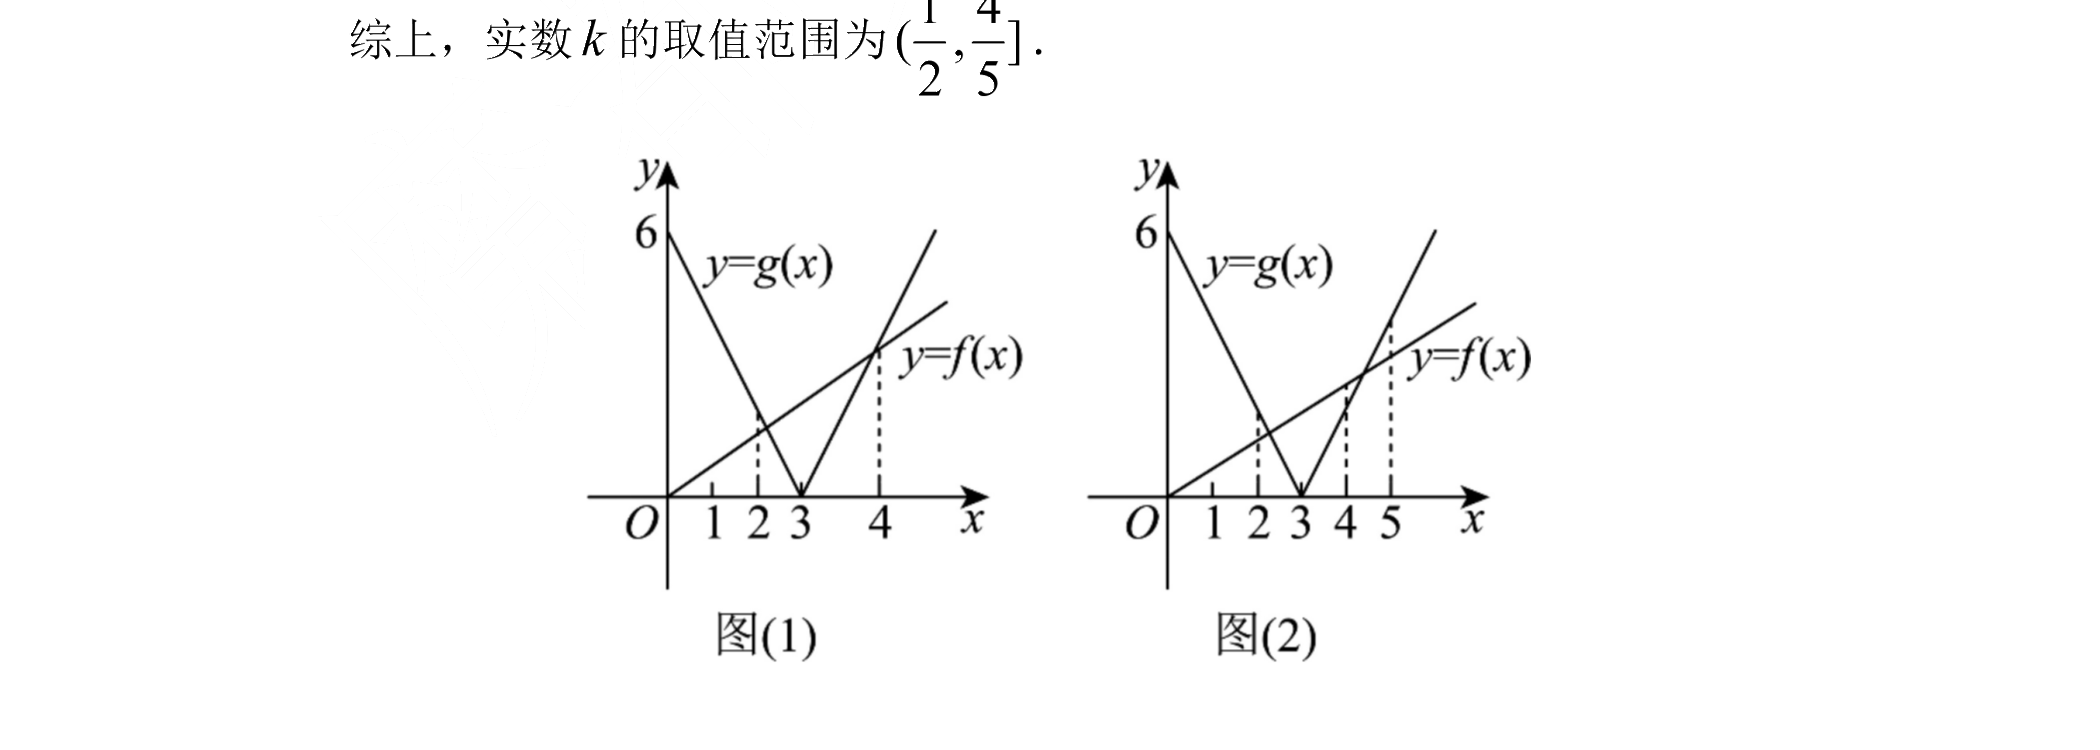
\includegraphics[width=0.72\textwidth]{figures/gao108_q11.png}
\end{center}

\step{综上，实数 $k$ 的取值范围为 $\left(\dfrac12,\dfrac45\right]$.}
\solend
\fi

\item 已知集合 $A=[1,a]\cup[a^3,a^4]$，集合 $B=\{x\mid x=x_1-x_2$，其中 $x_1$,$x_2\in A\}$. 若集合 $B$ 表
示的区间为一个闭区间，则实数 $a$ 的取值范围为\blankline[4.4em].

\ifanswer
\solbegin
\step{由题意得 $a^3>a>1$，则 $x_1-x_2$ 的最小值为 $1-a^4$，最大值为 $a^4-1$,}
\step{所以 $B=[1-a^4,a^4-1]$,}
\step{又因为 $a^4-a^3-(a-1)=a^3(a-1)-(a-1)=(a^3-1)(a-1)>0$,}
\step{所以 $a^4-a^3>a-1$，又集合 $B$ 表示的区间为一个闭区间,}
\step{则 $a^3-a\leqslant a^4-a^3$，化简得 $a^2-a-1\geqslant0$，又 $a>1$，解得 $a\geqslant\dfrac{1+\sqrt5}2$.}
\solend
\fi

\end{enumerate}

\bigsec{二、选择题}

\begin{enumerate}
\setcounter{enumi}{12}

\item 若 $a,b,c\in\R$，则下列不等式恒成立的是\mbox{（\quad）}% 原卷把答案“C”印在题干括号内、无【解析】

\keepwithprev
A. $\dfrac1a<\dfrac1b$\qquad B. $a^2<b^2$\qquad C. $\dfrac{a}{c^2+1}>\dfrac{b}{c^2+1}$\qquad D. $a\lvert c\rvert>b\lvert c\rvert$

\ifanswer
\ans{$C$}
\fi

\item 以下几个关系中正确的是\mbox{（\quad）}

\keepwithprev
A. $0\in\varnothing$\qquad\qquad\qquad B. $\varnothing\in\{x\mid x^2+1=0\}$

C. $\varnothing\subset\{0\}$\qquad\qquad\qquad D. $(A\cap B)\subset(A\cup B)$

\ifanswer
\solbegin
\step{$A$ 选项，$\varnothing$ 不包含任何元素，所以 $0\in\varnothing$ 错误，$A$ 错,}
\step{$B$ 选项，集合与集合之间关系不可以用 $\in$，$B$ 错,}
\step{$C$ 选项，空集是非空集合的真子集，所以 $\varnothing\subset\{0\}$ 正确，$C$ 对,}
\step{$D$ 选项，当 $A=B$ 时，$(A\cap B)=(A\cup B)$，$D$ 错,}
\step{故选 $C$.}
\solend
\fi

\item 设全集为 $U$，图中阴影部分所表示的集合是\mbox{（\quad）}% 原卷把答案“A”印在题干括号内、无【解析】

\keepwithprev
A. $B\cap\overline{A\cup C}$\qquad\qquad B. $(A\cup B)\cap(B\cup C)$

C. $(A\cup C)\cap\overline B$\qquad\qquad D. $(\overline A\cup\overline C)\cap B$

\ifanswer
\ans{$A$}
\fi

\item 对于 $k=0,1,2,\cdots$，定义集合 $A_k=\{20+k,26+2k\}$，并记 $S_k=A_0\cup A_1\cup\cdots\cup A_k$，则
使得集合 $S_n$ 中完全平方数的个数为奇数的最小正整数 $n$ 为\mbox{（\quad）}

\keepwithprev
A. $18$\qquad\qquad B. $19$\qquad\qquad C. $20$\qquad\qquad D. $21$

\ifanswer
\solbegin
\step{当 $k=0$ 时，$A_0=\{20,26\}$，对于 $k=0,1,2,\cdots$,}
\step{集合 $A_k$ 中最小的元素 $20>4^2$，若 $S_n$ 中完全平方数的个数为奇数，则 $n>4$,}
\step{（1）$20+k=5^2$ 时，$k=5$，$A_5=\{25,36\}$，此时 $S_5$ 中完全平方数为 $5^2$、$6^2$,}
\step{个数为 2;}
\step{$20+k=6^2$ 时，$k=16$，$A_{16}=\{36,58\}$，此时 $S_{16}$ 中完全平方数为 $5^2$、$6^2$,}
\step{个数为 2;}
\step{$20+k=7^2$ 时，$k=29$，$A_{29}=\{49,84\}$,}
\step{此时 $S_{29}$ 中完全平方数为 $5^2$、$6^2$、$7^2$、$8^2$，个数为 4;}
\step{$20+k=8^2$ 时，$k=44$，$A_{44}=\{64,114\}$,}
\step{此时 $S_{44}$ 中完全平方数为 $5^2$、$6^2$、$7^2$、$8^2$、$10^2$，个数为 5;}
\step{（2）因为 $k=0,1,2,\cdots,26+2k$ 一定为偶数,}
\step{所以 $26+2k=6^2$ 时，$k=5$，由上述分析得 $S_5$ 中完全平方数个数为 2;}
\step{$26+2k=8^2$ 时，$k=19$，$A_{19}=\{39,64\}$,}
\step{此时 $S_{19}$ 中完全平方数为 $5^2$、$6^2$、$8^2$，个数为 3.}
\step{综上，使集合 $S_n$ 中完全平方数的个数为奇数的最小正整数 $n=19$. 故选 $B$.}
\solend
\fi

\end{enumerate}

\bigsec{三、解答题}

\begin{enumerate}
\setcounter{enumi}{16}

\item 设全集 $U=\R$，集合 $A=\left\{x\,\middle|\,\dfrac{x-2}{x+2}\leqslant0\right\}$，$B=\{x\mid a\leqslant x<2a+1,a\in\R\}$，
$C=\{x\mid\lvert2x-1\rvert<5\}$.

（1）求集合 $A$、$\overline A\cup C$；

（2）若 $B\subseteq A$，求实数 $a$ 的取值范围.

\ifanswer
\solbegin
\ansspace*
\step{（1）不等式 $\dfrac{x-2}{x+2}\leqslant0$，等价于
$\begin{cases}(x-2)(x+2)\leqslant0\\x+2\neq0\end{cases}$，
解得 $\{x\mid-2<x\leqslant2\}$,}
\step{所以 $A=\{x\mid-2<x\leqslant2\}$，则 $\overline A=\{x\mid x\leqslant-2$ 或 $x>2\}$,}
\step{因为 $C=\{x\mid\lvert2x-1\rvert<5\}=\{x\mid-2<x<3\}$，所以 $\overline A\cup C=\R$；}
\step{（2）因为 $B\subseteq A$,}
\step{若 $B=\varnothing$，则 $a\geqslant2a+1$，解得 $a\leqslant-1$,}
\step{若 $B\neq\varnothing$，则
$\begin{cases}a<2a+1\\a>-2\\2a+1\leqslant2\end{cases}$，
解得 $-1<a\leqslant\dfrac12$,}
\step{综上所述，实数 $a$ 的取值范围为 $\left\{a\,\middle|\,a\leqslant\dfrac12\right\}$.}
\solend
\fi

\item 设 $a$、$b$、$c$、$d$ 是四个正数.

（1）已知 $a>b$，比较 $\dfrac{2a+b}{a+2b}$ 与 $\dfrac ab$ 的值的大小；

（2）若 $(1+a)(1+b)(1+c)(1+d)<16$，求证：$a$、$b$、$c$、$d$ 中至少有一个小于 1.

\ifanswer
\solbegin
\step{（1）$\dfrac{2a+b}{a+2b}-\dfrac ab=\dfrac{b^2-a^2}{b(a+2b)}<0$，所以 $\dfrac{2a+b}{a+2b}<\dfrac ab$.}
\step{（2）假设 $a$、$b$、$c$、$d$ 都不小于 1，即 $a$、$b$、$c$、$d$ 均大于等于 1,}
\step{即 $a\geqslant1$，$b\geqslant1$，$c\geqslant1$，$d\geqslant1$,}
\step{由均值不等式得 $1+a\geqslant2\sqrt a$,$1+b\geqslant2\sqrt b$,$1+c\geqslant2\sqrt c$,$1+d\geqslant2\sqrt d$,}
\step{故 $(1+a)(1+b)(1+c)(1+d)\geqslant16\sqrt{abcd}\geqslant16$,}
\step{当且仅当 $a=b=c=d=1$ 时取等号,}
\step{这与 $(1+a)(1+b)(1+c)(1+d)<16$ 矛盾，故假设不成立，原命题成立.}
\solend
\fi

\item 已知 $m\in\R$，一个二次项系数为 1 的一元二次方程的两个不等实根分别为 $x_1$ 和 $x_2$，且
满足
$\begin{cases}x_1^2+x_2^2=2m^2-4\\x_1+x_2=m\end{cases}$.

（1）直接写出该一元二次方程；

（2）若 $(3x_1-x_2)(3x_2-x_1)\geqslant-1$，求 $m$ 的取值范围；

（3）若方程的两根 $x_1$ 和 $x_2$ 都大于 $-1$，求 $m$ 的取值范围.

\ifanswer
\solbegin
\step{（1）设这个一元二次方程为 $x^2+bx+c=0$,}
\step{由
$\begin{cases}x_1^2+x_2^2=2m^2-4\\x_1+x_2=m\end{cases}$,}
\step{得 $(x_1+x_2)^2=x_1^2+x_2^2+2x_1x_2=2m^2-4+2x_1x_2=m^2$，即 $x_1x_2=\dfrac{4-m^2}2$,}
\step{由韦达定理得 $x_1+x_2=-b=m$，即 $x_1x_2=c=\dfrac{4-m^2}2$,}
\step{所以一元二次方程为 $x^2-mx+\dfrac{4-m^2}2=0$.}
\step{（2）$(3x_1-x_2)(3x_2-x_1)=9x_1x_2-3x_1^2-3x_2^2+x_1x_2=10x_1x_2-3(x_1^2+x_2^2)\geqslant-1$,}
\step{结合已知及（1）得 $x_1^2+x_2^2=2m^2-4$,$x_1x_2=\dfrac{4-m^2}2$,}
\step{代入得 $10\times\dfrac{4-m^2}2-3(2m^2-4)=-11m^2+32\geqslant-1\Rightarrow m^2\leqslant3$}
\step{$\Rightarrow-\sqrt3\leqslant m\leqslant\sqrt3$,}
\step{又 $\Delta=m^2-4\times\dfrac{4-m^2}2=3m^2-8>0\Rightarrow m<-\dfrac{2\sqrt6}3$ 或 $m>\dfrac{2\sqrt6}3$,}
\step{所以 $m\in\left[-\sqrt3,-\dfrac{2\sqrt6}3\right)\cup\left(\dfrac{2\sqrt6}3,\sqrt3\right]$.}
\step{（3）若方程的两根 $x_1$ 和 $x_2$ 都大于 $-1$，则
$\begin{cases}\Delta>0\\x_1+x_2>-2\\(x_1+1)(x_2+1)>0\end{cases}$,}
\step{所以
$\begin{cases}\Delta=3m^2-8>0\\m>-2\\[2pt]\dfrac{4-m^2}2+m+1>0\end{cases}$，
解得 $m\in\left(1-\sqrt7,-\dfrac{2\sqrt6}3\right)\cup\left(\dfrac{2\sqrt6}3,1+\sqrt7\right)$.}
\solend
\fi

\item 已知不等式 $2\leqslant ax^2+bx+c\leqslant3$ 的解集为 $\{x\mid2\leqslant x\leqslant3\}$.

（1）若 $a>0$，求 $6b+5c$ 的值；

（2）若 $a>0$，且不等式 $ax^2+(b-3)x-c\leqslant0$ 有且仅有 9 个整数解，求 $a$ 的取值范围；

（3）若 $a<0$，对任意的 $x<0$，不等式 $(ax-4)(x^2+b+c+1)\geqslant0$ 恒成立，求 $a^2-b+c$
的取值集合.

\ifanswer
\solbegin
\ansspace*
\step{（1）$a>0$,}
\step{结合二次函数图象得不等式 $ax^2+bx+c\leqslant3$ 的解集为 $\{x\mid2\leqslant x\leqslant3\}$,}
\step{且不等式 $ax^2+bx+c\geqslant2$ 的解集为 $R$,}
\step{所以方程 $ax^2+bx+c-3=0$ 的两根分别为 2 和 3,}
\step{则
$\begin{cases}2+3=-\dfrac ba\\[2pt]2\times3=\dfrac{c-3}a\end{cases}$，
得 $b=-5a$，$c=6a+3$,}
\step{所以 $6b+5c=6\times(-5a)+5(6a+3)=15$.}
\step{（2）若 $a>0$，且不等式 $ax^2+(b-3)x-c\leqslant0$ 有且仅有 9 个整数解,}
\step{由（1）得 $b=-5a$，$c=6a+3$,}
\step{不等式 $ax^2+bx+c\geqslant2$ 可化为 $ax^2-5ax+6a+1\geqslant0$.}
\step{由（1）得不等式 $ax^2+bx+c\geqslant2$ 的解集为 $R$,}
\step{所以 $ax^2-5ax+6a+1\geqslant0$ 恒成立,}
\step{所以
$\begin{cases}a>0\\\Delta=25a^2-4a(6a+1)\leqslant0\end{cases}$，
即
$\begin{cases}a>0\\a^2-4a=a(a-4)\leqslant0\end{cases}$，}
\step{解得 $0<a\leqslant4$.}
\step{不等式 $ax^2+(b-3)x-c\leqslant0$ 等价于 $ax^2-(5a+3)x-(6a+3)\leqslant0$,}
\step{所以 $[ax-(6a+3)](x+1)\leqslant0$，得 $-1\leqslant x\leqslant6+\dfrac3a$,}
\step{所以 $7\leqslant6+\dfrac3a<8$，解得 $\dfrac32<a\leqslant3$.}
\step{综上，$a$ 的取值范围为 $\left(\dfrac32,3\right]$.}
\step{（3）因为 $a<0$,}
\step{同（1）分析，不等式 $ax^2+bx+c\geqslant2$ 的解集为 $\{x\mid2\leqslant x\leqslant3\}$,}
\step{$ax^2+bx+c\leqslant3$ 的解集为 $R$,}
\step{所以方程 $ax^2+bx+c-2=0$ 的两根分别为 2 和 3,}
\step{则
$\begin{cases}2+3=-\dfrac ba\\[2pt]2\times3=\dfrac{c-2}a\end{cases}$，
得 $b=-5a$，$c=6a+2$.}
\step{所以不等式 $ax^2+bx+c=ax^2-5ax+6a+2\leqslant3$ 的解集为 $R$,}
\step{则 $ax^2-5ax+6a-1\leqslant0$ 恒成立,}
\step{所以
$\begin{cases}a<0\\\Delta=25a^2-4a(6a-1)\leqslant0\end{cases}$，
即
$\begin{cases}a<0\\a^2+4a=a(a+4)\leqslant0\end{cases}$，}
\step{解得 $-4\leqslant a<0$.}
\step{所以对任意的 $x<0$，不等式 $(ax-4)(x^2+b+c+1)\geqslant0$ 恒成立}
\step{转化为对任意的 $x<0$，不等式 $(ax-4)(x^2+a+3)\geqslant0$ 恒成立.}
\step{方程 $(ax-4)(x^2+a+3)=0$ 的两个根为 $x=\dfrac4a<0$,}
\step{$x=\pm\sqrt{-a-3}$（$a<-3$ 时成立）,}
\step{因而仅当 $ax-4=0$ 与 $x^2+a+3=0$ 的负根重合时满足条件,}
\step{解得唯一解为 $a=-4$，所以 $a^2-b+c=a^2+11a+2=-26$,}
\step{所以 $a^2-b+c$ 的取值集合为 $\{-26\}$.}
\solend
\fi

\item 已知集合 $A=\{1,2,3,4,5,6,7,8\}$，$M=\{(x,y)\mid x\in A,y\in A\}$，从 $M$ 中选取 $n$ 个不同的
元素组成一个序列：$(x_1,y_1)$,$(x_2,y_2),\cdots,(x_n,y_n)$，其中 $(x_i,y_i)$ 称为该序列的第 $i$ 项
（$i=1,2,\cdots,n$），若该序列的相邻项 $(x_i,y_i)$,$(x_{i+1},y_{i+1})$ 满足：
\[\begin{cases}\lvert x_{i+1}-x_i\rvert=3\\\lvert y_{i+1}-y_i\rvert=4\end{cases}
\quad\text{或}\quad
\begin{cases}\lvert x_{i+1}-x_i\rvert=4\\\lvert y_{i+1}-y_i\rvert=3\end{cases}\]
（$i=1,2,\cdots,n-1$），则称该序列为“$\Delta-$序列”.

（1）若一个 $\Delta-$序列的第一项为 $(4,4)$，请直接写出它所有可能的第二项；

（2）定义集合 $A=\{1,2,3,4,5,6,7,8\}$ 的两个子集：外侧集 $S=\{1,2,7,8\}$，内侧集
$T=\{3,4,5,6\}$. 证明：若 $\Delta-$序列中某一项的坐标在区域 $S\times S$ 内（即横、纵坐标均属于
$S$），则它的下一项坐标必定在区域 $T\times T$ 内；

（3）证明：不存在一个恰好有 5 项的 $\Delta-$序列，使其第一项为 $(1,8)$，且第五项为
$(8,1)$.

\ifanswer
\solbegin
\ansspace*
\step{（1）由题意，第一项为 $(x_1,y_1)=(4,4)$,}
\step{对于第二项 $(x_2,y_2)$，其坐标必须在 1~8 之间.}
\step{若 $\lvert x_2-4\rvert=3$,$\lvert y_2-4\rvert=4$，则 $x_2\in\{1,7\}$,}
\step{且 $y_2\in\{8\}$（因为 $4-4=0$ 不在集合 $A$ 中）. 此时可能的点为 $(1,8)$,$(7,8)$.}
\step{若 $\lvert x_2-4\rvert=4$,$\lvert y_2-4\rvert=3$，则 $x_2\in\{8\}$，且 $y_2\in\{1,7\}$.}
\step{此时可能的点为 $(8,1)$,$(8,7)$.}
\step{所以它所有可能的第二项为 $(1,8)$,$(7,8)$,$(8,1)$,$(8,7)$.}
\step{（2）已知某一项 $(x_t,y_t)\in S\times S$，即 $x_t\in\{1,2,7,8\}$ 且 $y_t\in\{1,2,7,8\}$.}
\step{由规则得下一步坐标的变化量为 3 和 4，设 $a\in S$ 变化 3 或 4 后的结果 $a'$:}
\step{当 $a=1$ 时，$1+3=4\in T$,$1+4=5\in T$；}
\step{当 $a=2$ 时，$2+3=5\in T$,$2+4=6\in T$；}
\step{当 $a=7$ 时，$7-3=4\in T$,$7-4=3\in T$；}
\step{当 $a=8$ 时，$8-3=5\in T$,$8-4=4\in T$.}
\step{（注：由于超出 1~8 范围的越界坐标不符合.）}
\step{由此可见，无论 $a$ 是 $S$ 中的哪一个数，加上或减去 3 或 4 之后,}
\step{得到的新坐标必属于集合 $T$.}
\step{因为 $\Delta-$序列每走一步，横坐标和纵坐标必定同时发生 3 和 4 的变化,}
\step{所以新的横坐标 $x_{i+1}$ 必属于 $T$，新的纵坐标 $y_{i+1}$ 也必属于 $T$,}
\step{即下一项 $(x_{i+1},y_{i+1})$ 必定在区域 $T\times T$ 内. ………10 分原命题得证.% 得分行混入证明，照录
}
\step{（3）假设存在这样一个包含 5 项的 $\Delta-$序列:}
\step{$(x_1,y_1)$,$(x_2,y_2)$,$(x_3,y_3)$,$(x_4,y_4)$,$(x_5,y_5)$.}
\step{已知第一项为 $(1,8)$，第五项为 $(8,1)$. 第 2 项必须是第 1 项 $(1,8)$ 的相邻点.}
\step{我们来找 $(1,8)$ 的相邻点：第 2 项只能是 $(4,4)$ 或 $(5,5)$,}
\step{第 4 项必须是第 5 项 $(8,1)$ 的相邻点（因为跳跃是双向可逆的）.}
\step{同理可算得，$(8,1)$ 的相邻点也只有两个：$(4,4)$ 和 $(5,5)$,}
\step{题目题干中明确规定，$\Delta-$序列由 $n$ 个不同的有序数对构成.% “题目题干”措辞重复，照录
}
\step{所以，第 2 项和第 4 项不能是同一个点. 这就意味着:}
\step{如果第 2 项是 $(4,4)$，第 4 项就必须是 $(5,5)$；反之亦然.}
\step{则第 3 项必须是 $(4,4)$ 和 $(5,5)$ 的公共相邻点.}
\step{$(4,4)$ 的相邻点集合为：$\{(1,8),(7,8),(8,1),(8,7)\}$,}
\step{$(5,5)$ 的相邻点集合为：$\{(2,1),(8,1),(1,2),(1,8)\}$,}
\step{所以，第 3 项只能填 $(1,8)$ 或者 $(8,1)$.}
\step{这与“序列由不同的有序数对构成”这一条件产生矛盾！}
\step{所以，不存在一个恰好有 5 项的 $\Delta-$序列,}
\step{使其第一项为 $(1,8)$，且第五项为 $(8,1)$.}
\solend
\fi

\end{enumerate}

\end{document}
"
%
% 原始材料：微信公众号“魔都数学加油站”文章，作者破晓，2026-11-03 17:19 发布；
% 连载“27学年高一108”，原文标题“27学年高一108——2026-2027年上海市五校联考高一上10月月考”；
% 原文链接：https://mp.weixin.qq.com/s/3nkP789Qar93NGMZXFFCSw。
% 正文为 14 张 PNG 页（第 2、3、6—13 页 4762×6735，第 1、4、5、14 页 2560×3620），
% 题目下印有【解析】，为讲评版。
% 题目、解析均据原图转录；卷面水印及公众号页脚未录入。
% 第 6 题解析的文氏图与第 11 题法二解析的两幅图象（图(1)、图(2)）裁自原图、去粉色水印
% 转灰度（gao108_q6.png、gao108_q11.png），第 6 题图属解析（仅答案版）、
% 第 11 题图属解析（仅答案版）。
%
% 卷首标题：原卷印作“2026-2027 年五校联考高一上 10 月月考”，标题下另印一行参与学校
% 名单“闵行中学、嘉定一中、松江一中、金山中学、嘉一实高”（全稿第 5 份原卷自印副标题，
% 按 14／24／49／50 成例照录，并登记进计数核对.py 的 SELFSUB）。
%
% 与原卷的排版差异：
%   ① 原文从第 3 题起，填空题编号为 3—12、选择题为 13—16、解答题为 17—21，本稿保留原题号；
%   ② 原卷每题下直接印【解析】，本稿按全稿惯例将解析置于答案版；第 4 题只印【答案】，
%      第 13、15 两题把答案印在题干括号内且无【解析】，均另提 \ans{}；
%   ③ 原卷副标题照录（见上）；
%   ④ 原卷填空横线按全稿惯例排为 \blankline[4.4em]；解答题按惯例加 \ansspace；选择题括号排
%      \mbox{（\quad）}、选项段前按惯例加 \keepwithprev；
%   ⑤ 原卷数集排斜体 $R$／$N$，按全稿惯例改 \R、\N。
%
% 原卷红色强调照录为黑体：第 11 题解析的“法一：”“法二：”原卷排红色，按 53 成例排
% \stepm{法一：}／\stepm{法二：}（加粗着色）。
%
% 原卷存疑：第 10 题题干“变项和”定义中“将 $M$ 中每个元素 $m$ 都乘以 $(-1)^n$ 后再求和”
% 的 $n$ 未加界定（据解析应为该元素在 $\{1,2,\cdots,2026\}$ 中的序号），照录。
% 第 21 题 (2) 解析末行“即下一项 $(x_{i+1},y_{i+1})$ 必定在区域 $T\times T$ 内. ………10 分
% 原命题得证.”，原卷把得分点行混入证明（“原命题”按上下文为“原命题的逆否”），照录。
% 第 21 题 (3) 解析“题目题干中明确规定”，“题目题干”措辞重复，照录。
%
% 行数核对：逐题数 \step/\stepm 条数，合计 164 条（Q3：3；Q4：0；Q5：2；Q6：1；Q7：3；
% Q8：3；Q9：3；Q10：6；Q11：21；Q12：5；Q13：0；Q14：5；Q15：0；Q16：15；Q17：7；
% Q18：7；Q19：13；Q20：34；Q21：36），与原卷印刷行逐题相等。第 4 题只印【答案】、
% 第 13、15 题括号内印答案，均提 \ans{}，不计入 \step 账。
%
\documentclass[a4paper,11pt]{article}
\usepackage{common}

\begin{document}

\examtitlest[3]{2026--2027 年五校联考高一上 10 月月考}{闵行中学、嘉定一中、松江一中、金山中学、嘉一实高}

\bigsec{一、填空题}

\begin{enumerate}
\setcounter{enumi}{2}

\item 已知等式 $2x^2+3x+5=2ax^2+a(3x+1)+c$ 恒成立，则实数 $a+c$ 的值为\blankline[4.4em].

\ifanswer
\solbegin
\step{因为 $2x^2+3x+5=2ax^2+a(3x+1)+c$ 恒成立,}
\step{即 $2x^2+3x+5=2ax^2+3ax+(a+c)$ 恒成立，所以
$\begin{cases}2=2a\\3=3a\\5=a+c\end{cases}$,}
\step{所以 $a+c=5$.}
\solend
\fi

\item 不等式 $\dfrac1x<\dfrac12$ 的解集是\blankline[4.4em].

\ifanswer
\ans{$(-\infty,0)\cup(2,+\infty)$}
\fi

\item 已知 $a$、$b$ 都是实数，则“$a^2=b^2$”是“$a^2+b^2=2ab$”的\blankline[4.4em]条件.

\ifanswer
\solbegin
\step{$a^2=b^2$ 等价于 $a=\pm b$；$a^2+b^2=2ab$ 等价于 $(a-b)^2=0$ 等价于 $a=b$,}
\step{故“$a^2=b^2$”是“$a^2+b^2=2ab$”的必要不充分条件.}
\solend
\fi

\item 已知全集 $U=\{x\mid x$ 为不大于 20 的素数$\}$，$A\cap\overline B=\{5\}$，$\overline A\cap B=\{3\}$，
$\overline{A\cup B}=\{7,13,17,19\}$，则 $A=$\blankline[4.4em].

\ifanswer
\solbegin
\step{如图所示，$A=\{2,5,11\}$.}

\begin{center}
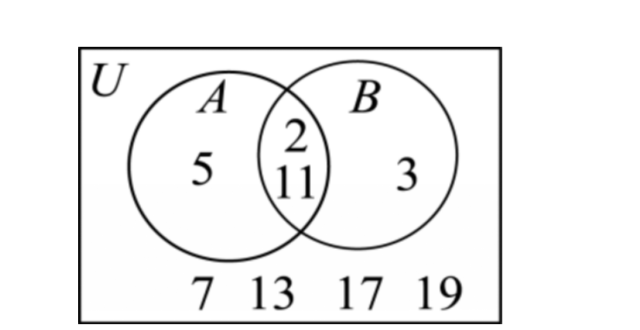
\includegraphics[width=0.24\textwidth]{figures/gao108_q6.png}
\end{center}

\solend
\fi

\item 若 $x\in A$，则 $\dfrac1x\in A$，就称 $A$ 自倒集合，集合 $M=\left\{-2,-1,0,\dfrac12,\dfrac13,1,2,3,4\right\}$ 的所有非空
子集中，自倒集合的个数为\blankline[4.4em].

\ifanswer
\solbegin
\step{由新定义，集合 $M$ 中的元素 1 和 $-1$ 倒数等于本身，2 和 $\dfrac12$，3 和 $\dfrac13$ 互为倒数,}
\step{故满足条件的自倒集合与集合 $\{-1,1,2,3\}$ 的非空子集的个数相同,}
\step{则其个数为 $2^4-1=15$.}
\solend
\fi

\item 设集合 $M=\{(x,y)\mid y=x^2+2bx+1\}$，$N=\{(x,y)\mid y=x+b\}(b\in\R)$，若
$M\cap N=\varnothing$，则实数 $b$ 的取值范围为\blankline[4.4em].

\ifanswer
\solbegin
\step{因为 $M\cap N=\varnothing$，所以
$\begin{cases}y=x^2+2bx+1\\y=x+b\end{cases}$
无解，则 $x^2+(2b-1)x+(1-b)=0$,}
\step{则 $\triangle=(2b-1)^2-4\times1\times(1-b)=4b^2-3<0$，解得 $-\dfrac{\sqrt3}2<b<\dfrac{\sqrt3}2$,}
\step{即实数 $b$ 的取值范围为 $\left(-\dfrac{\sqrt3}2,\dfrac{\sqrt3}2\right)$.}
\solend
\fi

\item 已知集合 $A=\left\{x\,\middle|\,\dfrac{x-a}{x^2-1}=1\right\}$ 有唯一元素，用列举法表示满足集合 $A$ 的条件的 $a$ 的取值集
合\blankline[4.4em].

\ifanswer
\solbegin
\step{$a=1$,$\dfrac{1}{x+1}=1$，一解；$a=-1$,$\dfrac{1}{x-1}=1$，一解；}
\step{$x-a=x^2-1$，一解时，$a=\dfrac54$,}
\step{综上，$a$ 的取值集合为 $\left\{-1,1,\dfrac54\right\}$.}
\solend
\fi

\item 已知集合 $M$ 的元素均为正整数，定义集合 $M$ 的“变项和”为：将 $M$ 中每个元素 $m$ 都乘
以 $(-1)^n$ 后再求和. 若集合 $A=\{n\mid1\leqslant n\leqslant2026,n\in\N\}$，则集合 $A$ 的所有非空子集的“变
项和”的总和为\blankline[4.4em].% $n$ 未加界定（据解析为元素序号），照录

\ifanswer
\solbegin
\step{$A=\{n\mid1\leqslant n\leqslant2026,n\in\N\}=\{1,2,\cdots,2026\}$,}
\step{1 在所有非空子集中共出现 $C_{2025}^{0}+C_{2025}^{1}+\cdots+C_{2025}^{2025}=2^{2025}$ 次,}
\step{同理 $2,3,\cdots,2026$ 都出现 $2^{2025}$ 次,}
\step{则集合 $A$ 的所有非空子集的“变项和”的总和}
\step{为 $2^{2025}\times[1\times(-1)^1+2\times(-1)^2+\cdots+2026\times(-1)^{2026}]$}
\step{$=2^{2025}\times(-1+2-3+4-\cdots-2025+2026)=1013\times2^{2025}$.}
\solend
\fi

\item 已知 $0<k<2$，定义 $[x]$ 为不超过 $x$ 的最大整数，区间 $[a,b]$（或 $(a,b)$，$[a,b)$，
$(a,b]$）的长度记为 $b-a$. 若关于 $x$ 的不等式 $k[x]>\lvert2[x]-6\rvert$ 的解集对应区间的长度为 $2$，
则 $k$ 的取值范围是\blankline[4.4em].

\ifanswer
\solbegin
\stepm{法一：}{由题意得 $\lvert2[x]-6\rvert=
\begin{cases}2[x]-6,x\geqslant3\\-2[x]+6,x<3\end{cases}$.}
\step{①当 $x\geqslant3$ 时，不等式 $k[x]>\lvert2[x]-6\rvert$ 可化为 $k[x]>2[x]-6$,}
\step{即 $(2-k)[x]<6$,}
\step{当 $0<k<2$ 时，解不等式 $(2-k)[x]<6$ 得 $[x]<\dfrac6{2-k}$.}
\step{②当 $x<3$ 时，不等式 $k[x]>\lvert2[x]-6\rvert$ 可化为 $k[x]>-2[x]+6$,}
\step{即 $(k+2)[x]>6$.}
\step{当 $0<k<2$ 时，解不等式 $(k+2)[x]>6$ 得 $[x]>\dfrac6{k+2}$.}
\step{综上所述，不等式 $k[x]>\lvert2[x]-6\rvert$ 的解集需满足 $\dfrac6{k+2}<[x]<\dfrac6{2-k}$,}
\step{由题意得在区间 $\left[\dfrac6{k+2},\dfrac6{2-k}\right]$ 内有两个整数,}
\step{由于 $\dfrac6{k+2}\in\left(\dfrac32,3\right)$，所以 $\dfrac6{2-k}\leqslant5$，得 $k\leqslant\dfrac45$.}
\step{因此 $k\in\left(0,\dfrac45\right]$，得 $\dfrac6{k+2}\in\left[\dfrac75,3\right)$，$\dfrac6{2-k}\in(3,5]$,}
\step{区间 $\left[\dfrac6{k+2},\dfrac6{2-k}\right]$ 内的两个整数是 3、4，所以 $4<\dfrac6{2-k}\leqslant5$，解得 $\dfrac12<k\leqslant\dfrac45$,}
\step{即 $k\in\left(\dfrac12,\dfrac45\right]$.}
\stepm{法二：}{令 $f(x)=kx$，$g(x)=\lvert2x-6\rvert$，画出 $g(x)$、$f(x)$ 的图象,}
\step{由于不等式 $k[x]>\lvert2[x]-6\rvert$ 的解集对应区间的长度为 2,}
\step{因此解集只可能为 $[3,5)$ 或 $[2,4)$.}
\step{当解集为 $[3,5)$ 时，如图（2），数形结合易得
$\begin{cases}f(2)\leqslant g(2)\\f(4)>g(4)\\f(5)\leqslant g(5)\end{cases}$,}
\step{即
$\begin{cases}2k\leqslant\lvert2\times2-6\rvert\\4k>\lvert2\times4-6\rvert\\5k\leqslant\lvert2\times5-6\rvert\end{cases}$，
解得
$\begin{cases}k\leqslant1\\k>\dfrac12\\k\leqslant\dfrac45\end{cases}$，
所以 $\dfrac12<k\leqslant\dfrac45$，满足 $0<k<2$,}
\step{当解集为 $[2,4)$ 时，如图（1），数形结合易得
$\begin{cases}f(2)>g(2)\\f(4)\leqslant g(4)\end{cases}$,}
\step{即
$\begin{cases}2k>\lvert2\times2-6\rvert\\4k\leqslant\lvert2\times4-6\rvert\end{cases}$，
无解.}

\begin{center}
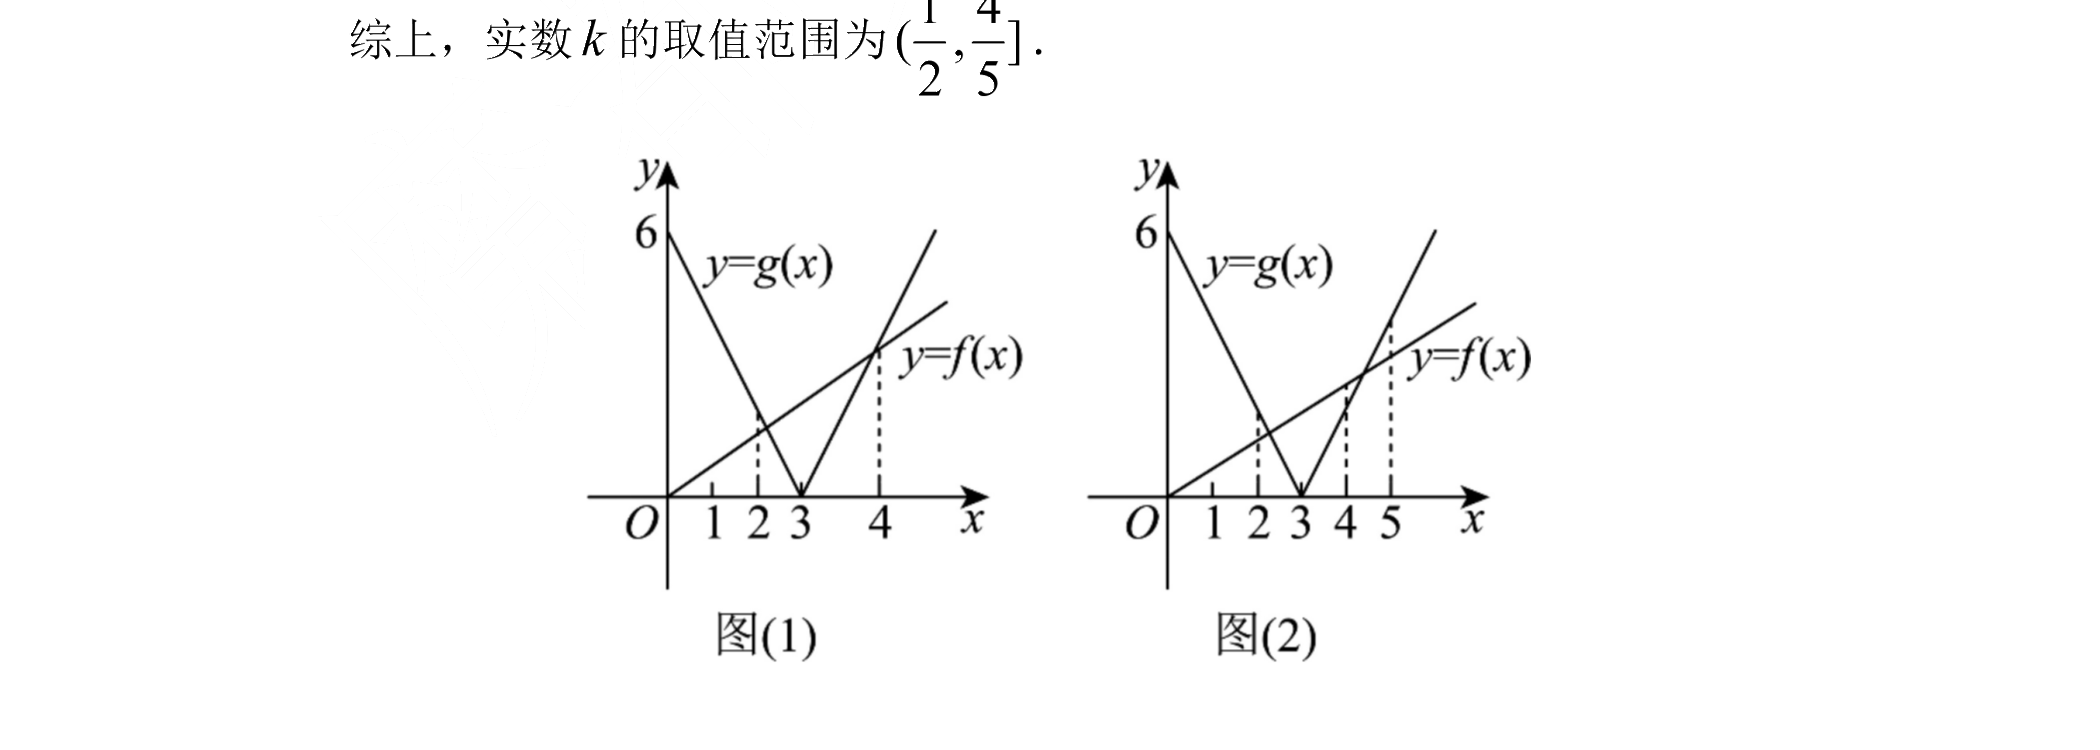
\includegraphics[width=0.72\textwidth]{figures/gao108_q11.png}
\end{center}

\step{综上，实数 $k$ 的取值范围为 $\left(\dfrac12,\dfrac45\right]$.}
\solend
\fi

\item 已知集合 $A=[1,a]\cup[a^3,a^4]$，集合 $B=\{x\mid x=x_1-x_2$，其中 $x_1$,$x_2\in A\}$. 若集合 $B$ 表
示的区间为一个闭区间，则实数 $a$ 的取值范围为\blankline[4.4em].

\ifanswer
\solbegin
\step{由题意得 $a^3>a>1$，则 $x_1-x_2$ 的最小值为 $1-a^4$，最大值为 $a^4-1$,}
\step{所以 $B=[1-a^4,a^4-1]$,}
\step{又因为 $a^4-a^3-(a-1)=a^3(a-1)-(a-1)=(a^3-1)(a-1)>0$,}
\step{所以 $a^4-a^3>a-1$，又集合 $B$ 表示的区间为一个闭区间,}
\step{则 $a^3-a\leqslant a^4-a^3$，化简得 $a^2-a-1\geqslant0$，又 $a>1$，解得 $a\geqslant\dfrac{1+\sqrt5}2$.}
\solend
\fi

\end{enumerate}

\bigsec{二、选择题}

\begin{enumerate}
\setcounter{enumi}{12}

\item 若 $a,b,c\in\R$，则下列不等式恒成立的是\mbox{（\quad）}% 原卷把答案“C”印在题干括号内、无【解析】

\keepwithprev
A. $\dfrac1a<\dfrac1b$\qquad B. $a^2<b^2$\qquad C. $\dfrac{a}{c^2+1}>\dfrac{b}{c^2+1}$\qquad D. $a\lvert c\rvert>b\lvert c\rvert$

\ifanswer
\ans{$C$}
\fi

\item 以下几个关系中正确的是\mbox{（\quad）}

\keepwithprev
A. $0\in\varnothing$\qquad\qquad\qquad B. $\varnothing\in\{x\mid x^2+1=0\}$

C. $\varnothing\subset\{0\}$\qquad\qquad\qquad D. $(A\cap B)\subset(A\cup B)$

\ifanswer
\solbegin
\step{$A$ 选项，$\varnothing$ 不包含任何元素，所以 $0\in\varnothing$ 错误，$A$ 错,}
\step{$B$ 选项，集合与集合之间关系不可以用 $\in$，$B$ 错,}
\step{$C$ 选项，空集是非空集合的真子集，所以 $\varnothing\subset\{0\}$ 正确，$C$ 对,}
\step{$D$ 选项，当 $A=B$ 时，$(A\cap B)=(A\cup B)$，$D$ 错,}
\step{故选 $C$.}
\solend
\fi

\item 设全集为 $U$，图中阴影部分所表示的集合是\mbox{（\quad）}% 原卷把答案“A”印在题干括号内、无【解析】

\keepwithprev
A. $B\cap\overline{A\cup C}$\qquad\qquad B. $(A\cup B)\cap(B\cup C)$

C. $(A\cup C)\cap\overline B$\qquad\qquad D. $(\overline A\cup\overline C)\cap B$

\ifanswer
\ans{$A$}
\fi

\item 对于 $k=0,1,2,\cdots$，定义集合 $A_k=\{20+k,26+2k\}$，并记 $S_k=A_0\cup A_1\cup\cdots\cup A_k$，则
使得集合 $S_n$ 中完全平方数的个数为奇数的最小正整数 $n$ 为\mbox{（\quad）}

\keepwithprev
A. $18$\qquad\qquad B. $19$\qquad\qquad C. $20$\qquad\qquad D. $21$

\ifanswer
\solbegin
\step{当 $k=0$ 时，$A_0=\{20,26\}$，对于 $k=0,1,2,\cdots$,}
\step{集合 $A_k$ 中最小的元素 $20>4^2$，若 $S_n$ 中完全平方数的个数为奇数，则 $n>4$,}
\step{（1）$20+k=5^2$ 时，$k=5$，$A_5=\{25,36\}$，此时 $S_5$ 中完全平方数为 $5^2$、$6^2$,}
\step{个数为 2;}
\step{$20+k=6^2$ 时，$k=16$，$A_{16}=\{36,58\}$，此时 $S_{16}$ 中完全平方数为 $5^2$、$6^2$,}
\step{个数为 2;}
\step{$20+k=7^2$ 时，$k=29$，$A_{29}=\{49,84\}$,}
\step{此时 $S_{29}$ 中完全平方数为 $5^2$、$6^2$、$7^2$、$8^2$，个数为 4;}
\step{$20+k=8^2$ 时，$k=44$，$A_{44}=\{64,114\}$,}
\step{此时 $S_{44}$ 中完全平方数为 $5^2$、$6^2$、$7^2$、$8^2$、$10^2$，个数为 5;}
\step{（2）因为 $k=0,1,2,\cdots,26+2k$ 一定为偶数,}
\step{所以 $26+2k=6^2$ 时，$k=5$，由上述分析得 $S_5$ 中完全平方数个数为 2;}
\step{$26+2k=8^2$ 时，$k=19$，$A_{19}=\{39,64\}$,}
\step{此时 $S_{19}$ 中完全平方数为 $5^2$、$6^2$、$8^2$，个数为 3.}
\step{综上，使集合 $S_n$ 中完全平方数的个数为奇数的最小正整数 $n=19$. 故选 $B$.}
\solend
\fi

\end{enumerate}

\bigsec{三、解答题}

\begin{enumerate}
\setcounter{enumi}{16}

\item 设全集 $U=\R$，集合 $A=\left\{x\,\middle|\,\dfrac{x-2}{x+2}\leqslant0\right\}$，$B=\{x\mid a\leqslant x<2a+1,a\in\R\}$，
$C=\{x\mid\lvert2x-1\rvert<5\}$.

（1）求集合 $A$、$\overline A\cup C$；

（2）若 $B\subseteq A$，求实数 $a$ 的取值范围.

\ifanswer
\solbegin
\ansspace*
\step{（1）不等式 $\dfrac{x-2}{x+2}\leqslant0$，等价于
$\begin{cases}(x-2)(x+2)\leqslant0\\x+2\neq0\end{cases}$，
解得 $\{x\mid-2<x\leqslant2\}$,}
\step{所以 $A=\{x\mid-2<x\leqslant2\}$，则 $\overline A=\{x\mid x\leqslant-2$ 或 $x>2\}$,}
\step{因为 $C=\{x\mid\lvert2x-1\rvert<5\}=\{x\mid-2<x<3\}$，所以 $\overline A\cup C=\R$；}
\step{（2）因为 $B\subseteq A$,}
\step{若 $B=\varnothing$，则 $a\geqslant2a+1$，解得 $a\leqslant-1$,}
\step{若 $B\neq\varnothing$，则
$\begin{cases}a<2a+1\\a>-2\\2a+1\leqslant2\end{cases}$，
解得 $-1<a\leqslant\dfrac12$,}
\step{综上所述，实数 $a$ 的取值范围为 $\left\{a\,\middle|\,a\leqslant\dfrac12\right\}$.}
\solend
\fi

\item 设 $a$、$b$、$c$、$d$ 是四个正数.

（1）已知 $a>b$，比较 $\dfrac{2a+b}{a+2b}$ 与 $\dfrac ab$ 的值的大小；

（2）若 $(1+a)(1+b)(1+c)(1+d)<16$，求证：$a$、$b$、$c$、$d$ 中至少有一个小于 1.

\ifanswer
\solbegin
\step{（1）$\dfrac{2a+b}{a+2b}-\dfrac ab=\dfrac{b^2-a^2}{b(a+2b)}<0$，所以 $\dfrac{2a+b}{a+2b}<\dfrac ab$.}
\step{（2）假设 $a$、$b$、$c$、$d$ 都不小于 1，即 $a$、$b$、$c$、$d$ 均大于等于 1,}
\step{即 $a\geqslant1$，$b\geqslant1$，$c\geqslant1$，$d\geqslant1$,}
\step{由均值不等式得 $1+a\geqslant2\sqrt a$,$1+b\geqslant2\sqrt b$,$1+c\geqslant2\sqrt c$,$1+d\geqslant2\sqrt d$,}
\step{故 $(1+a)(1+b)(1+c)(1+d)\geqslant16\sqrt{abcd}\geqslant16$,}
\step{当且仅当 $a=b=c=d=1$ 时取等号,}
\step{这与 $(1+a)(1+b)(1+c)(1+d)<16$ 矛盾，故假设不成立，原命题成立.}
\solend
\fi

\item 已知 $m\in\R$，一个二次项系数为 1 的一元二次方程的两个不等实根分别为 $x_1$ 和 $x_2$，且
满足
$\begin{cases}x_1^2+x_2^2=2m^2-4\\x_1+x_2=m\end{cases}$.

（1）直接写出该一元二次方程；

（2）若 $(3x_1-x_2)(3x_2-x_1)\geqslant-1$，求 $m$ 的取值范围；

（3）若方程的两根 $x_1$ 和 $x_2$ 都大于 $-1$，求 $m$ 的取值范围.

\ifanswer
\solbegin
\step{（1）设这个一元二次方程为 $x^2+bx+c=0$,}
\step{由
$\begin{cases}x_1^2+x_2^2=2m^2-4\\x_1+x_2=m\end{cases}$,}
\step{得 $(x_1+x_2)^2=x_1^2+x_2^2+2x_1x_2=2m^2-4+2x_1x_2=m^2$，即 $x_1x_2=\dfrac{4-m^2}2$,}
\step{由韦达定理得 $x_1+x_2=-b=m$，即 $x_1x_2=c=\dfrac{4-m^2}2$,}
\step{所以一元二次方程为 $x^2-mx+\dfrac{4-m^2}2=0$.}
\step{（2）$(3x_1-x_2)(3x_2-x_1)=9x_1x_2-3x_1^2-3x_2^2+x_1x_2=10x_1x_2-3(x_1^2+x_2^2)\geqslant-1$,}
\step{结合已知及（1）得 $x_1^2+x_2^2=2m^2-4$,$x_1x_2=\dfrac{4-m^2}2$,}
\step{代入得 $10\times\dfrac{4-m^2}2-3(2m^2-4)=-11m^2+32\geqslant-1\Rightarrow m^2\leqslant3$}
\step{$\Rightarrow-\sqrt3\leqslant m\leqslant\sqrt3$,}
\step{又 $\Delta=m^2-4\times\dfrac{4-m^2}2=3m^2-8>0\Rightarrow m<-\dfrac{2\sqrt6}3$ 或 $m>\dfrac{2\sqrt6}3$,}
\step{所以 $m\in\left[-\sqrt3,-\dfrac{2\sqrt6}3\right)\cup\left(\dfrac{2\sqrt6}3,\sqrt3\right]$.}
\step{（3）若方程的两根 $x_1$ 和 $x_2$ 都大于 $-1$，则
$\begin{cases}\Delta>0\\x_1+x_2>-2\\(x_1+1)(x_2+1)>0\end{cases}$,}
\step{所以
$\begin{cases}\Delta=3m^2-8>0\\m>-2\\[2pt]\dfrac{4-m^2}2+m+1>0\end{cases}$，
解得 $m\in\left(1-\sqrt7,-\dfrac{2\sqrt6}3\right)\cup\left(\dfrac{2\sqrt6}3,1+\sqrt7\right)$.}
\solend
\fi

\item 已知不等式 $2\leqslant ax^2+bx+c\leqslant3$ 的解集为 $\{x\mid2\leqslant x\leqslant3\}$.

（1）若 $a>0$，求 $6b+5c$ 的值；

（2）若 $a>0$，且不等式 $ax^2+(b-3)x-c\leqslant0$ 有且仅有 9 个整数解，求 $a$ 的取值范围；

（3）若 $a<0$，对任意的 $x<0$，不等式 $(ax-4)(x^2+b+c+1)\geqslant0$ 恒成立，求 $a^2-b+c$
的取值集合.

\ifanswer
\solbegin
\ansspace*
\step{（1）$a>0$,}
\step{结合二次函数图象得不等式 $ax^2+bx+c\leqslant3$ 的解集为 $\{x\mid2\leqslant x\leqslant3\}$,}
\step{且不等式 $ax^2+bx+c\geqslant2$ 的解集为 $R$,}
\step{所以方程 $ax^2+bx+c-3=0$ 的两根分别为 2 和 3,}
\step{则
$\begin{cases}2+3=-\dfrac ba\\[2pt]2\times3=\dfrac{c-3}a\end{cases}$，
得 $b=-5a$，$c=6a+3$,}
\step{所以 $6b+5c=6\times(-5a)+5(6a+3)=15$.}
\step{（2）若 $a>0$，且不等式 $ax^2+(b-3)x-c\leqslant0$ 有且仅有 9 个整数解,}
\step{由（1）得 $b=-5a$，$c=6a+3$,}
\step{不等式 $ax^2+bx+c\geqslant2$ 可化为 $ax^2-5ax+6a+1\geqslant0$.}
\step{由（1）得不等式 $ax^2+bx+c\geqslant2$ 的解集为 $R$,}
\step{所以 $ax^2-5ax+6a+1\geqslant0$ 恒成立,}
\step{所以
$\begin{cases}a>0\\\Delta=25a^2-4a(6a+1)\leqslant0\end{cases}$，
即
$\begin{cases}a>0\\a^2-4a=a(a-4)\leqslant0\end{cases}$，}
\step{解得 $0<a\leqslant4$.}
\step{不等式 $ax^2+(b-3)x-c\leqslant0$ 等价于 $ax^2-(5a+3)x-(6a+3)\leqslant0$,}
\step{所以 $[ax-(6a+3)](x+1)\leqslant0$，得 $-1\leqslant x\leqslant6+\dfrac3a$,}
\step{所以 $7\leqslant6+\dfrac3a<8$，解得 $\dfrac32<a\leqslant3$.}
\step{综上，$a$ 的取值范围为 $\left(\dfrac32,3\right]$.}
\step{（3）因为 $a<0$,}
\step{同（1）分析，不等式 $ax^2+bx+c\geqslant2$ 的解集为 $\{x\mid2\leqslant x\leqslant3\}$,}
\step{$ax^2+bx+c\leqslant3$ 的解集为 $R$,}
\step{所以方程 $ax^2+bx+c-2=0$ 的两根分别为 2 和 3,}
\step{则
$\begin{cases}2+3=-\dfrac ba\\[2pt]2\times3=\dfrac{c-2}a\end{cases}$，
得 $b=-5a$，$c=6a+2$.}
\step{所以不等式 $ax^2+bx+c=ax^2-5ax+6a+2\leqslant3$ 的解集为 $R$,}
\step{则 $ax^2-5ax+6a-1\leqslant0$ 恒成立,}
\step{所以
$\begin{cases}a<0\\\Delta=25a^2-4a(6a-1)\leqslant0\end{cases}$，
即
$\begin{cases}a<0\\a^2+4a=a(a+4)\leqslant0\end{cases}$，}
\step{解得 $-4\leqslant a<0$.}
\step{所以对任意的 $x<0$，不等式 $(ax-4)(x^2+b+c+1)\geqslant0$ 恒成立}
\step{转化为对任意的 $x<0$，不等式 $(ax-4)(x^2+a+3)\geqslant0$ 恒成立.}
\step{方程 $(ax-4)(x^2+a+3)=0$ 的两个根为 $x=\dfrac4a<0$,}
\step{$x=\pm\sqrt{-a-3}$（$a<-3$ 时成立）,}
\step{因而仅当 $ax-4=0$ 与 $x^2+a+3=0$ 的负根重合时满足条件,}
\step{解得唯一解为 $a=-4$，所以 $a^2-b+c=a^2+11a+2=-26$,}
\step{所以 $a^2-b+c$ 的取值集合为 $\{-26\}$.}
\solend
\fi

\item 已知集合 $A=\{1,2,3,4,5,6,7,8\}$，$M=\{(x,y)\mid x\in A,y\in A\}$，从 $M$ 中选取 $n$ 个不同的
元素组成一个序列：$(x_1,y_1)$,$(x_2,y_2),\cdots,(x_n,y_n)$，其中 $(x_i,y_i)$ 称为该序列的第 $i$ 项
（$i=1,2,\cdots,n$），若该序列的相邻项 $(x_i,y_i)$,$(x_{i+1},y_{i+1})$ 满足：
\[\begin{cases}\lvert x_{i+1}-x_i\rvert=3\\\lvert y_{i+1}-y_i\rvert=4\end{cases}
\quad\text{或}\quad
\begin{cases}\lvert x_{i+1}-x_i\rvert=4\\\lvert y_{i+1}-y_i\rvert=3\end{cases}\]
（$i=1,2,\cdots,n-1$），则称该序列为“$\Delta-$序列”.

（1）若一个 $\Delta-$序列的第一项为 $(4,4)$，请直接写出它所有可能的第二项；

（2）定义集合 $A=\{1,2,3,4,5,6,7,8\}$ 的两个子集：外侧集 $S=\{1,2,7,8\}$，内侧集
$T=\{3,4,5,6\}$. 证明：若 $\Delta-$序列中某一项的坐标在区域 $S\times S$ 内（即横、纵坐标均属于
$S$），则它的下一项坐标必定在区域 $T\times T$ 内；

（3）证明：不存在一个恰好有 5 项的 $\Delta-$序列，使其第一项为 $(1,8)$，且第五项为
$(8,1)$.

\ifanswer
\solbegin
\ansspace*
\step{（1）由题意，第一项为 $(x_1,y_1)=(4,4)$,}
\step{对于第二项 $(x_2,y_2)$，其坐标必须在 1~8 之间.}
\step{若 $\lvert x_2-4\rvert=3$,$\lvert y_2-4\rvert=4$，则 $x_2\in\{1,7\}$,}
\step{且 $y_2\in\{8\}$（因为 $4-4=0$ 不在集合 $A$ 中）. 此时可能的点为 $(1,8)$,$(7,8)$.}
\step{若 $\lvert x_2-4\rvert=4$,$\lvert y_2-4\rvert=3$，则 $x_2\in\{8\}$，且 $y_2\in\{1,7\}$.}
\step{此时可能的点为 $(8,1)$,$(8,7)$.}
\step{所以它所有可能的第二项为 $(1,8)$,$(7,8)$,$(8,1)$,$(8,7)$.}
\step{（2）已知某一项 $(x_t,y_t)\in S\times S$，即 $x_t\in\{1,2,7,8\}$ 且 $y_t\in\{1,2,7,8\}$.}
\step{由规则得下一步坐标的变化量为 3 和 4，设 $a\in S$ 变化 3 或 4 后的结果 $a'$:}
\step{当 $a=1$ 时，$1+3=4\in T$,$1+4=5\in T$；}
\step{当 $a=2$ 时，$2+3=5\in T$,$2+4=6\in T$；}
\step{当 $a=7$ 时，$7-3=4\in T$,$7-4=3\in T$；}
\step{当 $a=8$ 时，$8-3=5\in T$,$8-4=4\in T$.}
\step{（注：由于超出 1~8 范围的越界坐标不符合.）}
\step{由此可见，无论 $a$ 是 $S$ 中的哪一个数，加上或减去 3 或 4 之后,}
\step{得到的新坐标必属于集合 $T$.}
\step{因为 $\Delta-$序列每走一步，横坐标和纵坐标必定同时发生 3 和 4 的变化,}
\step{所以新的横坐标 $x_{i+1}$ 必属于 $T$，新的纵坐标 $y_{i+1}$ 也必属于 $T$,}
\step{即下一项 $(x_{i+1},y_{i+1})$ 必定在区域 $T\times T$ 内. ………10 分原命题得证.% 得分行混入证明，照录
}
\step{（3）假设存在这样一个包含 5 项的 $\Delta-$序列:}
\step{$(x_1,y_1)$,$(x_2,y_2)$,$(x_3,y_3)$,$(x_4,y_4)$,$(x_5,y_5)$.}
\step{已知第一项为 $(1,8)$，第五项为 $(8,1)$. 第 2 项必须是第 1 项 $(1,8)$ 的相邻点.}
\step{我们来找 $(1,8)$ 的相邻点：第 2 项只能是 $(4,4)$ 或 $(5,5)$,}
\step{第 4 项必须是第 5 项 $(8,1)$ 的相邻点（因为跳跃是双向可逆的）.}
\step{同理可算得，$(8,1)$ 的相邻点也只有两个：$(4,4)$ 和 $(5,5)$,}
\step{题目题干中明确规定，$\Delta-$序列由 $n$ 个不同的有序数对构成.% “题目题干”措辞重复，照录
}
\step{所以，第 2 项和第 4 项不能是同一个点. 这就意味着:}
\step{如果第 2 项是 $(4,4)$，第 4 项就必须是 $(5,5)$；反之亦然.}
\step{则第 3 项必须是 $(4,4)$ 和 $(5,5)$ 的公共相邻点.}
\step{$(4,4)$ 的相邻点集合为：$\{(1,8),(7,8),(8,1),(8,7)\}$,}
\step{$(5,5)$ 的相邻点集合为：$\{(2,1),(8,1),(1,2),(1,8)\}$,}
\step{所以，第 3 项只能填 $(1,8)$ 或者 $(8,1)$.}
\step{这与“序列由不同的有序数对构成”这一条件产生矛盾！}
\step{所以，不存在一个恰好有 5 项的 $\Delta-$序列,}
\step{使其第一项为 $(1,8)$，且第五项为 $(8,1)$.}
\solend
\fi

\end{enumerate}

\end{document}
"
% 紧凑版：xelatex "\def\iscompact{1}% 高一108_五校联考_10月月考.tex
%   —— 高一上数学“2026-2027 年五校联考高一上 10 月月考”（试卷版/答案版）
% 试卷版：xelatex 高一108_五校联考_10月月考.tex
% 答案版：xelatex "\def\isanswer{1}% 高一108_五校联考_10月月考.tex
%   —— 高一上数学“2026-2027 年五校联考高一上 10 月月考”（试卷版/答案版）
% 试卷版：xelatex 高一108_五校联考_10月月考.tex
% 答案版：xelatex "\def\isanswer{1}\input{高一108_五校联考_10月月考.tex}"
% 紧凑版：xelatex "\def\iscompact{1}\input{高一108_五校联考_10月月考.tex}"
%
% 原始材料：微信公众号“魔都数学加油站”文章，作者破晓，2026-11-03 17:19 发布；
% 连载“27学年高一108”，原文标题“27学年高一108——2026-2027年上海市五校联考高一上10月月考”；
% 原文链接：https://mp.weixin.qq.com/s/3nkP789Qar93NGMZXFFCSw。
% 正文为 14 张 PNG 页（第 2、3、6—13 页 4762×6735，第 1、4、5、14 页 2560×3620），
% 题目下印有【解析】，为讲评版。
% 题目、解析均据原图转录；卷面水印及公众号页脚未录入。
% 第 6 题解析的文氏图与第 11 题法二解析的两幅图象（图(1)、图(2)）裁自原图、去粉色水印
% 转灰度（gao108_q6.png、gao108_q11.png），第 6 题图属解析（仅答案版）、
% 第 11 题图属解析（仅答案版）。
%
% 卷首标题：原卷印作“2026-2027 年五校联考高一上 10 月月考”，标题下另印一行参与学校
% 名单“闵行中学、嘉定一中、松江一中、金山中学、嘉一实高”（全稿第 5 份原卷自印副标题，
% 按 14／24／49／50 成例照录，并登记进计数核对.py 的 SELFSUB）。
%
% 与原卷的排版差异：
%   ① 原文从第 3 题起，填空题编号为 3—12、选择题为 13—16、解答题为 17—21，本稿保留原题号；
%   ② 原卷每题下直接印【解析】，本稿按全稿惯例将解析置于答案版；第 4 题只印【答案】，
%      第 13、15 两题把答案印在题干括号内且无【解析】，均另提 \ans{}；
%   ③ 原卷副标题照录（见上）；
%   ④ 原卷填空横线按全稿惯例排为 \blankline[4.4em]；解答题按惯例加 \ansspace；选择题括号排
%      \mbox{（\quad）}、选项段前按惯例加 \keepwithprev；
%   ⑤ 原卷数集排斜体 $R$／$N$，按全稿惯例改 \R、\N。
%
% 原卷红色强调照录为黑体：第 11 题解析的“法一：”“法二：”原卷排红色，按 53 成例排
% \stepm{法一：}／\stepm{法二：}（加粗着色）。
%
% 原卷存疑：第 10 题题干“变项和”定义中“将 $M$ 中每个元素 $m$ 都乘以 $(-1)^n$ 后再求和”
% 的 $n$ 未加界定（据解析应为该元素在 $\{1,2,\cdots,2026\}$ 中的序号），照录。
% 第 21 题 (2) 解析末行“即下一项 $(x_{i+1},y_{i+1})$ 必定在区域 $T\times T$ 内. ………10 分
% 原命题得证.”，原卷把得分点行混入证明（“原命题”按上下文为“原命题的逆否”），照录。
% 第 21 题 (3) 解析“题目题干中明确规定”，“题目题干”措辞重复，照录。
%
% 行数核对：逐题数 \step/\stepm 条数，合计 164 条（Q3：3；Q4：0；Q5：2；Q6：1；Q7：3；
% Q8：3；Q9：3；Q10：6；Q11：21；Q12：5；Q13：0；Q14：5；Q15：0；Q16：15；Q17：7；
% Q18：7；Q19：13；Q20：34；Q21：36），与原卷印刷行逐题相等。第 4 题只印【答案】、
% 第 13、15 题括号内印答案，均提 \ans{}，不计入 \step 账。
%
\documentclass[a4paper,11pt]{article}
\usepackage{common}

\begin{document}

\examtitlest[3]{2026--2027 年五校联考高一上 10 月月考}{闵行中学、嘉定一中、松江一中、金山中学、嘉一实高}

\bigsec{一、填空题}

\begin{enumerate}
\setcounter{enumi}{2}

\item 已知等式 $2x^2+3x+5=2ax^2+a(3x+1)+c$ 恒成立，则实数 $a+c$ 的值为\blankline[4.4em].

\ifanswer
\solbegin
\step{因为 $2x^2+3x+5=2ax^2+a(3x+1)+c$ 恒成立,}
\step{即 $2x^2+3x+5=2ax^2+3ax+(a+c)$ 恒成立，所以
$\begin{cases}2=2a\\3=3a\\5=a+c\end{cases}$,}
\step{所以 $a+c=5$.}
\solend
\fi

\item 不等式 $\dfrac1x<\dfrac12$ 的解集是\blankline[4.4em].

\ifanswer
\ans{$(-\infty,0)\cup(2,+\infty)$}
\fi

\item 已知 $a$、$b$ 都是实数，则“$a^2=b^2$”是“$a^2+b^2=2ab$”的\blankline[4.4em]条件.

\ifanswer
\solbegin
\step{$a^2=b^2$ 等价于 $a=\pm b$；$a^2+b^2=2ab$ 等价于 $(a-b)^2=0$ 等价于 $a=b$,}
\step{故“$a^2=b^2$”是“$a^2+b^2=2ab$”的必要不充分条件.}
\solend
\fi

\item 已知全集 $U=\{x\mid x$ 为不大于 20 的素数$\}$，$A\cap\overline B=\{5\}$，$\overline A\cap B=\{3\}$，
$\overline{A\cup B}=\{7,13,17,19\}$，则 $A=$\blankline[4.4em].

\ifanswer
\solbegin
\step{如图所示，$A=\{2,5,11\}$.}

\begin{center}
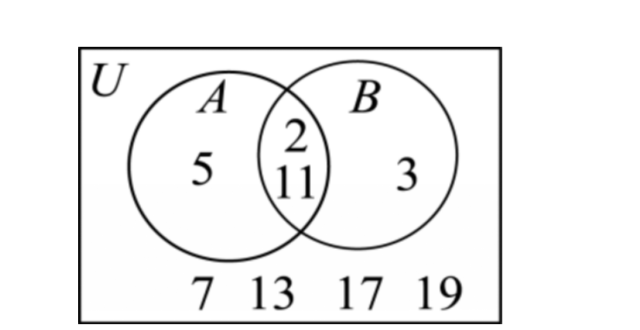
\includegraphics[width=0.24\textwidth]{figures/gao108_q6.png}
\end{center}

\solend
\fi

\item 若 $x\in A$，则 $\dfrac1x\in A$，就称 $A$ 自倒集合，集合 $M=\left\{-2,-1,0,\dfrac12,\dfrac13,1,2,3,4\right\}$ 的所有非空
子集中，自倒集合的个数为\blankline[4.4em].

\ifanswer
\solbegin
\step{由新定义，集合 $M$ 中的元素 1 和 $-1$ 倒数等于本身，2 和 $\dfrac12$，3 和 $\dfrac13$ 互为倒数,}
\step{故满足条件的自倒集合与集合 $\{-1,1,2,3\}$ 的非空子集的个数相同,}
\step{则其个数为 $2^4-1=15$.}
\solend
\fi

\item 设集合 $M=\{(x,y)\mid y=x^2+2bx+1\}$，$N=\{(x,y)\mid y=x+b\}(b\in\R)$，若
$M\cap N=\varnothing$，则实数 $b$ 的取值范围为\blankline[4.4em].

\ifanswer
\solbegin
\step{因为 $M\cap N=\varnothing$，所以
$\begin{cases}y=x^2+2bx+1\\y=x+b\end{cases}$
无解，则 $x^2+(2b-1)x+(1-b)=0$,}
\step{则 $\triangle=(2b-1)^2-4\times1\times(1-b)=4b^2-3<0$，解得 $-\dfrac{\sqrt3}2<b<\dfrac{\sqrt3}2$,}
\step{即实数 $b$ 的取值范围为 $\left(-\dfrac{\sqrt3}2,\dfrac{\sqrt3}2\right)$.}
\solend
\fi

\item 已知集合 $A=\left\{x\,\middle|\,\dfrac{x-a}{x^2-1}=1\right\}$ 有唯一元素，用列举法表示满足集合 $A$ 的条件的 $a$ 的取值集
合\blankline[4.4em].

\ifanswer
\solbegin
\step{$a=1$,$\dfrac{1}{x+1}=1$，一解；$a=-1$,$\dfrac{1}{x-1}=1$，一解；}
\step{$x-a=x^2-1$，一解时，$a=\dfrac54$,}
\step{综上，$a$ 的取值集合为 $\left\{-1,1,\dfrac54\right\}$.}
\solend
\fi

\item 已知集合 $M$ 的元素均为正整数，定义集合 $M$ 的“变项和”为：将 $M$ 中每个元素 $m$ 都乘
以 $(-1)^n$ 后再求和. 若集合 $A=\{n\mid1\leqslant n\leqslant2026,n\in\N\}$，则集合 $A$ 的所有非空子集的“变
项和”的总和为\blankline[4.4em].% $n$ 未加界定（据解析为元素序号），照录

\ifanswer
\solbegin
\step{$A=\{n\mid1\leqslant n\leqslant2026,n\in\N\}=\{1,2,\cdots,2026\}$,}
\step{1 在所有非空子集中共出现 $C_{2025}^{0}+C_{2025}^{1}+\cdots+C_{2025}^{2025}=2^{2025}$ 次,}
\step{同理 $2,3,\cdots,2026$ 都出现 $2^{2025}$ 次,}
\step{则集合 $A$ 的所有非空子集的“变项和”的总和}
\step{为 $2^{2025}\times[1\times(-1)^1+2\times(-1)^2+\cdots+2026\times(-1)^{2026}]$}
\step{$=2^{2025}\times(-1+2-3+4-\cdots-2025+2026)=1013\times2^{2025}$.}
\solend
\fi

\item 已知 $0<k<2$，定义 $[x]$ 为不超过 $x$ 的最大整数，区间 $[a,b]$（或 $(a,b)$，$[a,b)$，
$(a,b]$）的长度记为 $b-a$. 若关于 $x$ 的不等式 $k[x]>\lvert2[x]-6\rvert$ 的解集对应区间的长度为 $2$，
则 $k$ 的取值范围是\blankline[4.4em].

\ifanswer
\solbegin
\stepm{法一：}{由题意得 $\lvert2[x]-6\rvert=
\begin{cases}2[x]-6,x\geqslant3\\-2[x]+6,x<3\end{cases}$.}
\step{①当 $x\geqslant3$ 时，不等式 $k[x]>\lvert2[x]-6\rvert$ 可化为 $k[x]>2[x]-6$,}
\step{即 $(2-k)[x]<6$,}
\step{当 $0<k<2$ 时，解不等式 $(2-k)[x]<6$ 得 $[x]<\dfrac6{2-k}$.}
\step{②当 $x<3$ 时，不等式 $k[x]>\lvert2[x]-6\rvert$ 可化为 $k[x]>-2[x]+6$,}
\step{即 $(k+2)[x]>6$.}
\step{当 $0<k<2$ 时，解不等式 $(k+2)[x]>6$ 得 $[x]>\dfrac6{k+2}$.}
\step{综上所述，不等式 $k[x]>\lvert2[x]-6\rvert$ 的解集需满足 $\dfrac6{k+2}<[x]<\dfrac6{2-k}$,}
\step{由题意得在区间 $\left[\dfrac6{k+2},\dfrac6{2-k}\right]$ 内有两个整数,}
\step{由于 $\dfrac6{k+2}\in\left(\dfrac32,3\right)$，所以 $\dfrac6{2-k}\leqslant5$，得 $k\leqslant\dfrac45$.}
\step{因此 $k\in\left(0,\dfrac45\right]$，得 $\dfrac6{k+2}\in\left[\dfrac75,3\right)$，$\dfrac6{2-k}\in(3,5]$,}
\step{区间 $\left[\dfrac6{k+2},\dfrac6{2-k}\right]$ 内的两个整数是 3、4，所以 $4<\dfrac6{2-k}\leqslant5$，解得 $\dfrac12<k\leqslant\dfrac45$,}
\step{即 $k\in\left(\dfrac12,\dfrac45\right]$.}
\stepm{法二：}{令 $f(x)=kx$，$g(x)=\lvert2x-6\rvert$，画出 $g(x)$、$f(x)$ 的图象,}
\step{由于不等式 $k[x]>\lvert2[x]-6\rvert$ 的解集对应区间的长度为 2,}
\step{因此解集只可能为 $[3,5)$ 或 $[2,4)$.}
\step{当解集为 $[3,5)$ 时，如图（2），数形结合易得
$\begin{cases}f(2)\leqslant g(2)\\f(4)>g(4)\\f(5)\leqslant g(5)\end{cases}$,}
\step{即
$\begin{cases}2k\leqslant\lvert2\times2-6\rvert\\4k>\lvert2\times4-6\rvert\\5k\leqslant\lvert2\times5-6\rvert\end{cases}$，
解得
$\begin{cases}k\leqslant1\\k>\dfrac12\\k\leqslant\dfrac45\end{cases}$，
所以 $\dfrac12<k\leqslant\dfrac45$，满足 $0<k<2$,}
\step{当解集为 $[2,4)$ 时，如图（1），数形结合易得
$\begin{cases}f(2)>g(2)\\f(4)\leqslant g(4)\end{cases}$,}
\step{即
$\begin{cases}2k>\lvert2\times2-6\rvert\\4k\leqslant\lvert2\times4-6\rvert\end{cases}$，
无解.}

\begin{center}
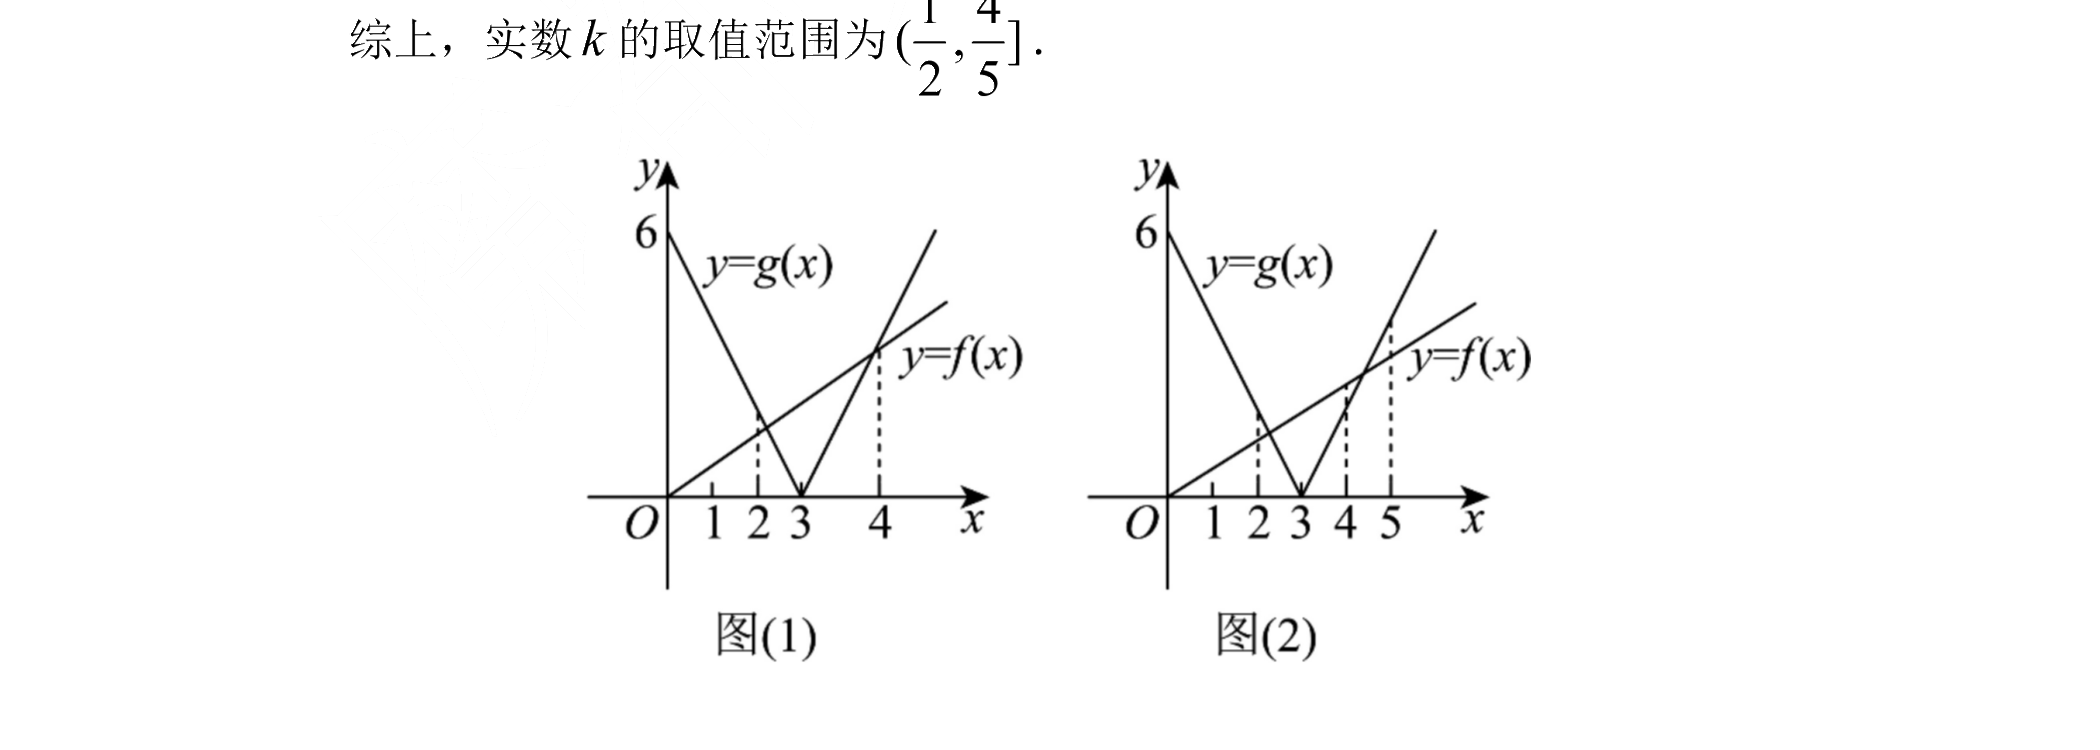
\includegraphics[width=0.72\textwidth]{figures/gao108_q11.png}
\end{center}

\step{综上，实数 $k$ 的取值范围为 $\left(\dfrac12,\dfrac45\right]$.}
\solend
\fi

\item 已知集合 $A=[1,a]\cup[a^3,a^4]$，集合 $B=\{x\mid x=x_1-x_2$，其中 $x_1$,$x_2\in A\}$. 若集合 $B$ 表
示的区间为一个闭区间，则实数 $a$ 的取值范围为\blankline[4.4em].

\ifanswer
\solbegin
\step{由题意得 $a^3>a>1$，则 $x_1-x_2$ 的最小值为 $1-a^4$，最大值为 $a^4-1$,}
\step{所以 $B=[1-a^4,a^4-1]$,}
\step{又因为 $a^4-a^3-(a-1)=a^3(a-1)-(a-1)=(a^3-1)(a-1)>0$,}
\step{所以 $a^4-a^3>a-1$，又集合 $B$ 表示的区间为一个闭区间,}
\step{则 $a^3-a\leqslant a^4-a^3$，化简得 $a^2-a-1\geqslant0$，又 $a>1$，解得 $a\geqslant\dfrac{1+\sqrt5}2$.}
\solend
\fi

\end{enumerate}

\bigsec{二、选择题}

\begin{enumerate}
\setcounter{enumi}{12}

\item 若 $a,b,c\in\R$，则下列不等式恒成立的是\mbox{（\quad）}% 原卷把答案“C”印在题干括号内、无【解析】

\keepwithprev
A. $\dfrac1a<\dfrac1b$\qquad B. $a^2<b^2$\qquad C. $\dfrac{a}{c^2+1}>\dfrac{b}{c^2+1}$\qquad D. $a\lvert c\rvert>b\lvert c\rvert$

\ifanswer
\ans{$C$}
\fi

\item 以下几个关系中正确的是\mbox{（\quad）}

\keepwithprev
A. $0\in\varnothing$\qquad\qquad\qquad B. $\varnothing\in\{x\mid x^2+1=0\}$

C. $\varnothing\subset\{0\}$\qquad\qquad\qquad D. $(A\cap B)\subset(A\cup B)$

\ifanswer
\solbegin
\step{$A$ 选项，$\varnothing$ 不包含任何元素，所以 $0\in\varnothing$ 错误，$A$ 错,}
\step{$B$ 选项，集合与集合之间关系不可以用 $\in$，$B$ 错,}
\step{$C$ 选项，空集是非空集合的真子集，所以 $\varnothing\subset\{0\}$ 正确，$C$ 对,}
\step{$D$ 选项，当 $A=B$ 时，$(A\cap B)=(A\cup B)$，$D$ 错,}
\step{故选 $C$.}
\solend
\fi

\item 设全集为 $U$，图中阴影部分所表示的集合是\mbox{（\quad）}% 原卷把答案“A”印在题干括号内、无【解析】

\keepwithprev
A. $B\cap\overline{A\cup C}$\qquad\qquad B. $(A\cup B)\cap(B\cup C)$

C. $(A\cup C)\cap\overline B$\qquad\qquad D. $(\overline A\cup\overline C)\cap B$

\ifanswer
\ans{$A$}
\fi

\item 对于 $k=0,1,2,\cdots$，定义集合 $A_k=\{20+k,26+2k\}$，并记 $S_k=A_0\cup A_1\cup\cdots\cup A_k$，则
使得集合 $S_n$ 中完全平方数的个数为奇数的最小正整数 $n$ 为\mbox{（\quad）}

\keepwithprev
A. $18$\qquad\qquad B. $19$\qquad\qquad C. $20$\qquad\qquad D. $21$

\ifanswer
\solbegin
\step{当 $k=0$ 时，$A_0=\{20,26\}$，对于 $k=0,1,2,\cdots$,}
\step{集合 $A_k$ 中最小的元素 $20>4^2$，若 $S_n$ 中完全平方数的个数为奇数，则 $n>4$,}
\step{（1）$20+k=5^2$ 时，$k=5$，$A_5=\{25,36\}$，此时 $S_5$ 中完全平方数为 $5^2$、$6^2$,}
\step{个数为 2;}
\step{$20+k=6^2$ 时，$k=16$，$A_{16}=\{36,58\}$，此时 $S_{16}$ 中完全平方数为 $5^2$、$6^2$,}
\step{个数为 2;}
\step{$20+k=7^2$ 时，$k=29$，$A_{29}=\{49,84\}$,}
\step{此时 $S_{29}$ 中完全平方数为 $5^2$、$6^2$、$7^2$、$8^2$，个数为 4;}
\step{$20+k=8^2$ 时，$k=44$，$A_{44}=\{64,114\}$,}
\step{此时 $S_{44}$ 中完全平方数为 $5^2$、$6^2$、$7^2$、$8^2$、$10^2$，个数为 5;}
\step{（2）因为 $k=0,1,2,\cdots,26+2k$ 一定为偶数,}
\step{所以 $26+2k=6^2$ 时，$k=5$，由上述分析得 $S_5$ 中完全平方数个数为 2;}
\step{$26+2k=8^2$ 时，$k=19$，$A_{19}=\{39,64\}$,}
\step{此时 $S_{19}$ 中完全平方数为 $5^2$、$6^2$、$8^2$，个数为 3.}
\step{综上，使集合 $S_n$ 中完全平方数的个数为奇数的最小正整数 $n=19$. 故选 $B$.}
\solend
\fi

\end{enumerate}

\bigsec{三、解答题}

\begin{enumerate}
\setcounter{enumi}{16}

\item 设全集 $U=\R$，集合 $A=\left\{x\,\middle|\,\dfrac{x-2}{x+2}\leqslant0\right\}$，$B=\{x\mid a\leqslant x<2a+1,a\in\R\}$，
$C=\{x\mid\lvert2x-1\rvert<5\}$.

（1）求集合 $A$、$\overline A\cup C$；

（2）若 $B\subseteq A$，求实数 $a$ 的取值范围.

\ifanswer
\solbegin
\ansspace*
\step{（1）不等式 $\dfrac{x-2}{x+2}\leqslant0$，等价于
$\begin{cases}(x-2)(x+2)\leqslant0\\x+2\neq0\end{cases}$，
解得 $\{x\mid-2<x\leqslant2\}$,}
\step{所以 $A=\{x\mid-2<x\leqslant2\}$，则 $\overline A=\{x\mid x\leqslant-2$ 或 $x>2\}$,}
\step{因为 $C=\{x\mid\lvert2x-1\rvert<5\}=\{x\mid-2<x<3\}$，所以 $\overline A\cup C=\R$；}
\step{（2）因为 $B\subseteq A$,}
\step{若 $B=\varnothing$，则 $a\geqslant2a+1$，解得 $a\leqslant-1$,}
\step{若 $B\neq\varnothing$，则
$\begin{cases}a<2a+1\\a>-2\\2a+1\leqslant2\end{cases}$，
解得 $-1<a\leqslant\dfrac12$,}
\step{综上所述，实数 $a$ 的取值范围为 $\left\{a\,\middle|\,a\leqslant\dfrac12\right\}$.}
\solend
\fi

\item 设 $a$、$b$、$c$、$d$ 是四个正数.

（1）已知 $a>b$，比较 $\dfrac{2a+b}{a+2b}$ 与 $\dfrac ab$ 的值的大小；

（2）若 $(1+a)(1+b)(1+c)(1+d)<16$，求证：$a$、$b$、$c$、$d$ 中至少有一个小于 1.

\ifanswer
\solbegin
\step{（1）$\dfrac{2a+b}{a+2b}-\dfrac ab=\dfrac{b^2-a^2}{b(a+2b)}<0$，所以 $\dfrac{2a+b}{a+2b}<\dfrac ab$.}
\step{（2）假设 $a$、$b$、$c$、$d$ 都不小于 1，即 $a$、$b$、$c$、$d$ 均大于等于 1,}
\step{即 $a\geqslant1$，$b\geqslant1$，$c\geqslant1$，$d\geqslant1$,}
\step{由均值不等式得 $1+a\geqslant2\sqrt a$,$1+b\geqslant2\sqrt b$,$1+c\geqslant2\sqrt c$,$1+d\geqslant2\sqrt d$,}
\step{故 $(1+a)(1+b)(1+c)(1+d)\geqslant16\sqrt{abcd}\geqslant16$,}
\step{当且仅当 $a=b=c=d=1$ 时取等号,}
\step{这与 $(1+a)(1+b)(1+c)(1+d)<16$ 矛盾，故假设不成立，原命题成立.}
\solend
\fi

\item 已知 $m\in\R$，一个二次项系数为 1 的一元二次方程的两个不等实根分别为 $x_1$ 和 $x_2$，且
满足
$\begin{cases}x_1^2+x_2^2=2m^2-4\\x_1+x_2=m\end{cases}$.

（1）直接写出该一元二次方程；

（2）若 $(3x_1-x_2)(3x_2-x_1)\geqslant-1$，求 $m$ 的取值范围；

（3）若方程的两根 $x_1$ 和 $x_2$ 都大于 $-1$，求 $m$ 的取值范围.

\ifanswer
\solbegin
\step{（1）设这个一元二次方程为 $x^2+bx+c=0$,}
\step{由
$\begin{cases}x_1^2+x_2^2=2m^2-4\\x_1+x_2=m\end{cases}$,}
\step{得 $(x_1+x_2)^2=x_1^2+x_2^2+2x_1x_2=2m^2-4+2x_1x_2=m^2$，即 $x_1x_2=\dfrac{4-m^2}2$,}
\step{由韦达定理得 $x_1+x_2=-b=m$，即 $x_1x_2=c=\dfrac{4-m^2}2$,}
\step{所以一元二次方程为 $x^2-mx+\dfrac{4-m^2}2=0$.}
\step{（2）$(3x_1-x_2)(3x_2-x_1)=9x_1x_2-3x_1^2-3x_2^2+x_1x_2=10x_1x_2-3(x_1^2+x_2^2)\geqslant-1$,}
\step{结合已知及（1）得 $x_1^2+x_2^2=2m^2-4$,$x_1x_2=\dfrac{4-m^2}2$,}
\step{代入得 $10\times\dfrac{4-m^2}2-3(2m^2-4)=-11m^2+32\geqslant-1\Rightarrow m^2\leqslant3$}
\step{$\Rightarrow-\sqrt3\leqslant m\leqslant\sqrt3$,}
\step{又 $\Delta=m^2-4\times\dfrac{4-m^2}2=3m^2-8>0\Rightarrow m<-\dfrac{2\sqrt6}3$ 或 $m>\dfrac{2\sqrt6}3$,}
\step{所以 $m\in\left[-\sqrt3,-\dfrac{2\sqrt6}3\right)\cup\left(\dfrac{2\sqrt6}3,\sqrt3\right]$.}
\step{（3）若方程的两根 $x_1$ 和 $x_2$ 都大于 $-1$，则
$\begin{cases}\Delta>0\\x_1+x_2>-2\\(x_1+1)(x_2+1)>0\end{cases}$,}
\step{所以
$\begin{cases}\Delta=3m^2-8>0\\m>-2\\[2pt]\dfrac{4-m^2}2+m+1>0\end{cases}$，
解得 $m\in\left(1-\sqrt7,-\dfrac{2\sqrt6}3\right)\cup\left(\dfrac{2\sqrt6}3,1+\sqrt7\right)$.}
\solend
\fi

\item 已知不等式 $2\leqslant ax^2+bx+c\leqslant3$ 的解集为 $\{x\mid2\leqslant x\leqslant3\}$.

（1）若 $a>0$，求 $6b+5c$ 的值；

（2）若 $a>0$，且不等式 $ax^2+(b-3)x-c\leqslant0$ 有且仅有 9 个整数解，求 $a$ 的取值范围；

（3）若 $a<0$，对任意的 $x<0$，不等式 $(ax-4)(x^2+b+c+1)\geqslant0$ 恒成立，求 $a^2-b+c$
的取值集合.

\ifanswer
\solbegin
\ansspace*
\step{（1）$a>0$,}
\step{结合二次函数图象得不等式 $ax^2+bx+c\leqslant3$ 的解集为 $\{x\mid2\leqslant x\leqslant3\}$,}
\step{且不等式 $ax^2+bx+c\geqslant2$ 的解集为 $R$,}
\step{所以方程 $ax^2+bx+c-3=0$ 的两根分别为 2 和 3,}
\step{则
$\begin{cases}2+3=-\dfrac ba\\[2pt]2\times3=\dfrac{c-3}a\end{cases}$，
得 $b=-5a$，$c=6a+3$,}
\step{所以 $6b+5c=6\times(-5a)+5(6a+3)=15$.}
\step{（2）若 $a>0$，且不等式 $ax^2+(b-3)x-c\leqslant0$ 有且仅有 9 个整数解,}
\step{由（1）得 $b=-5a$，$c=6a+3$,}
\step{不等式 $ax^2+bx+c\geqslant2$ 可化为 $ax^2-5ax+6a+1\geqslant0$.}
\step{由（1）得不等式 $ax^2+bx+c\geqslant2$ 的解集为 $R$,}
\step{所以 $ax^2-5ax+6a+1\geqslant0$ 恒成立,}
\step{所以
$\begin{cases}a>0\\\Delta=25a^2-4a(6a+1)\leqslant0\end{cases}$，
即
$\begin{cases}a>0\\a^2-4a=a(a-4)\leqslant0\end{cases}$，}
\step{解得 $0<a\leqslant4$.}
\step{不等式 $ax^2+(b-3)x-c\leqslant0$ 等价于 $ax^2-(5a+3)x-(6a+3)\leqslant0$,}
\step{所以 $[ax-(6a+3)](x+1)\leqslant0$，得 $-1\leqslant x\leqslant6+\dfrac3a$,}
\step{所以 $7\leqslant6+\dfrac3a<8$，解得 $\dfrac32<a\leqslant3$.}
\step{综上，$a$ 的取值范围为 $\left(\dfrac32,3\right]$.}
\step{（3）因为 $a<0$,}
\step{同（1）分析，不等式 $ax^2+bx+c\geqslant2$ 的解集为 $\{x\mid2\leqslant x\leqslant3\}$,}
\step{$ax^2+bx+c\leqslant3$ 的解集为 $R$,}
\step{所以方程 $ax^2+bx+c-2=0$ 的两根分别为 2 和 3,}
\step{则
$\begin{cases}2+3=-\dfrac ba\\[2pt]2\times3=\dfrac{c-2}a\end{cases}$，
得 $b=-5a$，$c=6a+2$.}
\step{所以不等式 $ax^2+bx+c=ax^2-5ax+6a+2\leqslant3$ 的解集为 $R$,}
\step{则 $ax^2-5ax+6a-1\leqslant0$ 恒成立,}
\step{所以
$\begin{cases}a<0\\\Delta=25a^2-4a(6a-1)\leqslant0\end{cases}$，
即
$\begin{cases}a<0\\a^2+4a=a(a+4)\leqslant0\end{cases}$，}
\step{解得 $-4\leqslant a<0$.}
\step{所以对任意的 $x<0$，不等式 $(ax-4)(x^2+b+c+1)\geqslant0$ 恒成立}
\step{转化为对任意的 $x<0$，不等式 $(ax-4)(x^2+a+3)\geqslant0$ 恒成立.}
\step{方程 $(ax-4)(x^2+a+3)=0$ 的两个根为 $x=\dfrac4a<0$,}
\step{$x=\pm\sqrt{-a-3}$（$a<-3$ 时成立）,}
\step{因而仅当 $ax-4=0$ 与 $x^2+a+3=0$ 的负根重合时满足条件,}
\step{解得唯一解为 $a=-4$，所以 $a^2-b+c=a^2+11a+2=-26$,}
\step{所以 $a^2-b+c$ 的取值集合为 $\{-26\}$.}
\solend
\fi

\item 已知集合 $A=\{1,2,3,4,5,6,7,8\}$，$M=\{(x,y)\mid x\in A,y\in A\}$，从 $M$ 中选取 $n$ 个不同的
元素组成一个序列：$(x_1,y_1)$,$(x_2,y_2),\cdots,(x_n,y_n)$，其中 $(x_i,y_i)$ 称为该序列的第 $i$ 项
（$i=1,2,\cdots,n$），若该序列的相邻项 $(x_i,y_i)$,$(x_{i+1},y_{i+1})$ 满足：
\[\begin{cases}\lvert x_{i+1}-x_i\rvert=3\\\lvert y_{i+1}-y_i\rvert=4\end{cases}
\quad\text{或}\quad
\begin{cases}\lvert x_{i+1}-x_i\rvert=4\\\lvert y_{i+1}-y_i\rvert=3\end{cases}\]
（$i=1,2,\cdots,n-1$），则称该序列为“$\Delta-$序列”.

（1）若一个 $\Delta-$序列的第一项为 $(4,4)$，请直接写出它所有可能的第二项；

（2）定义集合 $A=\{1,2,3,4,5,6,7,8\}$ 的两个子集：外侧集 $S=\{1,2,7,8\}$，内侧集
$T=\{3,4,5,6\}$. 证明：若 $\Delta-$序列中某一项的坐标在区域 $S\times S$ 内（即横、纵坐标均属于
$S$），则它的下一项坐标必定在区域 $T\times T$ 内；

（3）证明：不存在一个恰好有 5 项的 $\Delta-$序列，使其第一项为 $(1,8)$，且第五项为
$(8,1)$.

\ifanswer
\solbegin
\ansspace*
\step{（1）由题意，第一项为 $(x_1,y_1)=(4,4)$,}
\step{对于第二项 $(x_2,y_2)$，其坐标必须在 1~8 之间.}
\step{若 $\lvert x_2-4\rvert=3$,$\lvert y_2-4\rvert=4$，则 $x_2\in\{1,7\}$,}
\step{且 $y_2\in\{8\}$（因为 $4-4=0$ 不在集合 $A$ 中）. 此时可能的点为 $(1,8)$,$(7,8)$.}
\step{若 $\lvert x_2-4\rvert=4$,$\lvert y_2-4\rvert=3$，则 $x_2\in\{8\}$，且 $y_2\in\{1,7\}$.}
\step{此时可能的点为 $(8,1)$,$(8,7)$.}
\step{所以它所有可能的第二项为 $(1,8)$,$(7,8)$,$(8,1)$,$(8,7)$.}
\step{（2）已知某一项 $(x_t,y_t)\in S\times S$，即 $x_t\in\{1,2,7,8\}$ 且 $y_t\in\{1,2,7,8\}$.}
\step{由规则得下一步坐标的变化量为 3 和 4，设 $a\in S$ 变化 3 或 4 后的结果 $a'$:}
\step{当 $a=1$ 时，$1+3=4\in T$,$1+4=5\in T$；}
\step{当 $a=2$ 时，$2+3=5\in T$,$2+4=6\in T$；}
\step{当 $a=7$ 时，$7-3=4\in T$,$7-4=3\in T$；}
\step{当 $a=8$ 时，$8-3=5\in T$,$8-4=4\in T$.}
\step{（注：由于超出 1~8 范围的越界坐标不符合.）}
\step{由此可见，无论 $a$ 是 $S$ 中的哪一个数，加上或减去 3 或 4 之后,}
\step{得到的新坐标必属于集合 $T$.}
\step{因为 $\Delta-$序列每走一步，横坐标和纵坐标必定同时发生 3 和 4 的变化,}
\step{所以新的横坐标 $x_{i+1}$ 必属于 $T$，新的纵坐标 $y_{i+1}$ 也必属于 $T$,}
\step{即下一项 $(x_{i+1},y_{i+1})$ 必定在区域 $T\times T$ 内. ………10 分原命题得证.% 得分行混入证明，照录
}
\step{（3）假设存在这样一个包含 5 项的 $\Delta-$序列:}
\step{$(x_1,y_1)$,$(x_2,y_2)$,$(x_3,y_3)$,$(x_4,y_4)$,$(x_5,y_5)$.}
\step{已知第一项为 $(1,8)$，第五项为 $(8,1)$. 第 2 项必须是第 1 项 $(1,8)$ 的相邻点.}
\step{我们来找 $(1,8)$ 的相邻点：第 2 项只能是 $(4,4)$ 或 $(5,5)$,}
\step{第 4 项必须是第 5 项 $(8,1)$ 的相邻点（因为跳跃是双向可逆的）.}
\step{同理可算得，$(8,1)$ 的相邻点也只有两个：$(4,4)$ 和 $(5,5)$,}
\step{题目题干中明确规定，$\Delta-$序列由 $n$ 个不同的有序数对构成.% “题目题干”措辞重复，照录
}
\step{所以，第 2 项和第 4 项不能是同一个点. 这就意味着:}
\step{如果第 2 项是 $(4,4)$，第 4 项就必须是 $(5,5)$；反之亦然.}
\step{则第 3 项必须是 $(4,4)$ 和 $(5,5)$ 的公共相邻点.}
\step{$(4,4)$ 的相邻点集合为：$\{(1,8),(7,8),(8,1),(8,7)\}$,}
\step{$(5,5)$ 的相邻点集合为：$\{(2,1),(8,1),(1,2),(1,8)\}$,}
\step{所以，第 3 项只能填 $(1,8)$ 或者 $(8,1)$.}
\step{这与“序列由不同的有序数对构成”这一条件产生矛盾！}
\step{所以，不存在一个恰好有 5 项的 $\Delta-$序列,}
\step{使其第一项为 $(1,8)$，且第五项为 $(8,1)$.}
\solend
\fi

\end{enumerate}

\end{document}
"
% 紧凑版：xelatex "\def\iscompact{1}% 高一108_五校联考_10月月考.tex
%   —— 高一上数学“2026-2027 年五校联考高一上 10 月月考”（试卷版/答案版）
% 试卷版：xelatex 高一108_五校联考_10月月考.tex
% 答案版：xelatex "\def\isanswer{1}\input{高一108_五校联考_10月月考.tex}"
% 紧凑版：xelatex "\def\iscompact{1}\input{高一108_五校联考_10月月考.tex}"
%
% 原始材料：微信公众号“魔都数学加油站”文章，作者破晓，2026-11-03 17:19 发布；
% 连载“27学年高一108”，原文标题“27学年高一108——2026-2027年上海市五校联考高一上10月月考”；
% 原文链接：https://mp.weixin.qq.com/s/3nkP789Qar93NGMZXFFCSw。
% 正文为 14 张 PNG 页（第 2、3、6—13 页 4762×6735，第 1、4、5、14 页 2560×3620），
% 题目下印有【解析】，为讲评版。
% 题目、解析均据原图转录；卷面水印及公众号页脚未录入。
% 第 6 题解析的文氏图与第 11 题法二解析的两幅图象（图(1)、图(2)）裁自原图、去粉色水印
% 转灰度（gao108_q6.png、gao108_q11.png），第 6 题图属解析（仅答案版）、
% 第 11 题图属解析（仅答案版）。
%
% 卷首标题：原卷印作“2026-2027 年五校联考高一上 10 月月考”，标题下另印一行参与学校
% 名单“闵行中学、嘉定一中、松江一中、金山中学、嘉一实高”（全稿第 5 份原卷自印副标题，
% 按 14／24／49／50 成例照录，并登记进计数核对.py 的 SELFSUB）。
%
% 与原卷的排版差异：
%   ① 原文从第 3 题起，填空题编号为 3—12、选择题为 13—16、解答题为 17—21，本稿保留原题号；
%   ② 原卷每题下直接印【解析】，本稿按全稿惯例将解析置于答案版；第 4 题只印【答案】，
%      第 13、15 两题把答案印在题干括号内且无【解析】，均另提 \ans{}；
%   ③ 原卷副标题照录（见上）；
%   ④ 原卷填空横线按全稿惯例排为 \blankline[4.4em]；解答题按惯例加 \ansspace；选择题括号排
%      \mbox{（\quad）}、选项段前按惯例加 \keepwithprev；
%   ⑤ 原卷数集排斜体 $R$／$N$，按全稿惯例改 \R、\N。
%
% 原卷红色强调照录为黑体：第 11 题解析的“法一：”“法二：”原卷排红色，按 53 成例排
% \stepm{法一：}／\stepm{法二：}（加粗着色）。
%
% 原卷存疑：第 10 题题干“变项和”定义中“将 $M$ 中每个元素 $m$ 都乘以 $(-1)^n$ 后再求和”
% 的 $n$ 未加界定（据解析应为该元素在 $\{1,2,\cdots,2026\}$ 中的序号），照录。
% 第 21 题 (2) 解析末行“即下一项 $(x_{i+1},y_{i+1})$ 必定在区域 $T\times T$ 内. ………10 分
% 原命题得证.”，原卷把得分点行混入证明（“原命题”按上下文为“原命题的逆否”），照录。
% 第 21 题 (3) 解析“题目题干中明确规定”，“题目题干”措辞重复，照录。
%
% 行数核对：逐题数 \step/\stepm 条数，合计 164 条（Q3：3；Q4：0；Q5：2；Q6：1；Q7：3；
% Q8：3；Q9：3；Q10：6；Q11：21；Q12：5；Q13：0；Q14：5；Q15：0；Q16：15；Q17：7；
% Q18：7；Q19：13；Q20：34；Q21：36），与原卷印刷行逐题相等。第 4 题只印【答案】、
% 第 13、15 题括号内印答案，均提 \ans{}，不计入 \step 账。
%
\documentclass[a4paper,11pt]{article}
\usepackage{common}

\begin{document}

\examtitlest[3]{2026--2027 年五校联考高一上 10 月月考}{闵行中学、嘉定一中、松江一中、金山中学、嘉一实高}

\bigsec{一、填空题}

\begin{enumerate}
\setcounter{enumi}{2}

\item 已知等式 $2x^2+3x+5=2ax^2+a(3x+1)+c$ 恒成立，则实数 $a+c$ 的值为\blankline[4.4em].

\ifanswer
\solbegin
\step{因为 $2x^2+3x+5=2ax^2+a(3x+1)+c$ 恒成立,}
\step{即 $2x^2+3x+5=2ax^2+3ax+(a+c)$ 恒成立，所以
$\begin{cases}2=2a\\3=3a\\5=a+c\end{cases}$,}
\step{所以 $a+c=5$.}
\solend
\fi

\item 不等式 $\dfrac1x<\dfrac12$ 的解集是\blankline[4.4em].

\ifanswer
\ans{$(-\infty,0)\cup(2,+\infty)$}
\fi

\item 已知 $a$、$b$ 都是实数，则“$a^2=b^2$”是“$a^2+b^2=2ab$”的\blankline[4.4em]条件.

\ifanswer
\solbegin
\step{$a^2=b^2$ 等价于 $a=\pm b$；$a^2+b^2=2ab$ 等价于 $(a-b)^2=0$ 等价于 $a=b$,}
\step{故“$a^2=b^2$”是“$a^2+b^2=2ab$”的必要不充分条件.}
\solend
\fi

\item 已知全集 $U=\{x\mid x$ 为不大于 20 的素数$\}$，$A\cap\overline B=\{5\}$，$\overline A\cap B=\{3\}$，
$\overline{A\cup B}=\{7,13,17,19\}$，则 $A=$\blankline[4.4em].

\ifanswer
\solbegin
\step{如图所示，$A=\{2,5,11\}$.}

\begin{center}
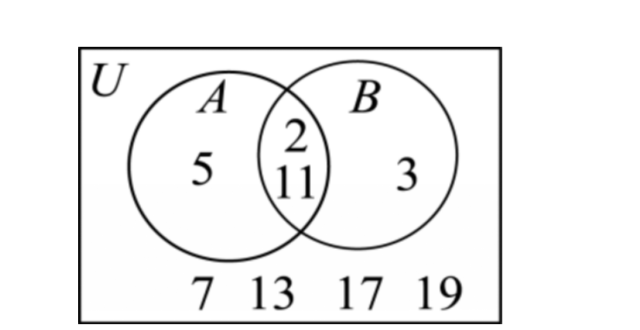
\includegraphics[width=0.24\textwidth]{figures/gao108_q6.png}
\end{center}

\solend
\fi

\item 若 $x\in A$，则 $\dfrac1x\in A$，就称 $A$ 自倒集合，集合 $M=\left\{-2,-1,0,\dfrac12,\dfrac13,1,2,3,4\right\}$ 的所有非空
子集中，自倒集合的个数为\blankline[4.4em].

\ifanswer
\solbegin
\step{由新定义，集合 $M$ 中的元素 1 和 $-1$ 倒数等于本身，2 和 $\dfrac12$，3 和 $\dfrac13$ 互为倒数,}
\step{故满足条件的自倒集合与集合 $\{-1,1,2,3\}$ 的非空子集的个数相同,}
\step{则其个数为 $2^4-1=15$.}
\solend
\fi

\item 设集合 $M=\{(x,y)\mid y=x^2+2bx+1\}$，$N=\{(x,y)\mid y=x+b\}(b\in\R)$，若
$M\cap N=\varnothing$，则实数 $b$ 的取值范围为\blankline[4.4em].

\ifanswer
\solbegin
\step{因为 $M\cap N=\varnothing$，所以
$\begin{cases}y=x^2+2bx+1\\y=x+b\end{cases}$
无解，则 $x^2+(2b-1)x+(1-b)=0$,}
\step{则 $\triangle=(2b-1)^2-4\times1\times(1-b)=4b^2-3<0$，解得 $-\dfrac{\sqrt3}2<b<\dfrac{\sqrt3}2$,}
\step{即实数 $b$ 的取值范围为 $\left(-\dfrac{\sqrt3}2,\dfrac{\sqrt3}2\right)$.}
\solend
\fi

\item 已知集合 $A=\left\{x\,\middle|\,\dfrac{x-a}{x^2-1}=1\right\}$ 有唯一元素，用列举法表示满足集合 $A$ 的条件的 $a$ 的取值集
合\blankline[4.4em].

\ifanswer
\solbegin
\step{$a=1$,$\dfrac{1}{x+1}=1$，一解；$a=-1$,$\dfrac{1}{x-1}=1$，一解；}
\step{$x-a=x^2-1$，一解时，$a=\dfrac54$,}
\step{综上，$a$ 的取值集合为 $\left\{-1,1,\dfrac54\right\}$.}
\solend
\fi

\item 已知集合 $M$ 的元素均为正整数，定义集合 $M$ 的“变项和”为：将 $M$ 中每个元素 $m$ 都乘
以 $(-1)^n$ 后再求和. 若集合 $A=\{n\mid1\leqslant n\leqslant2026,n\in\N\}$，则集合 $A$ 的所有非空子集的“变
项和”的总和为\blankline[4.4em].% $n$ 未加界定（据解析为元素序号），照录

\ifanswer
\solbegin
\step{$A=\{n\mid1\leqslant n\leqslant2026,n\in\N\}=\{1,2,\cdots,2026\}$,}
\step{1 在所有非空子集中共出现 $C_{2025}^{0}+C_{2025}^{1}+\cdots+C_{2025}^{2025}=2^{2025}$ 次,}
\step{同理 $2,3,\cdots,2026$ 都出现 $2^{2025}$ 次,}
\step{则集合 $A$ 的所有非空子集的“变项和”的总和}
\step{为 $2^{2025}\times[1\times(-1)^1+2\times(-1)^2+\cdots+2026\times(-1)^{2026}]$}
\step{$=2^{2025}\times(-1+2-3+4-\cdots-2025+2026)=1013\times2^{2025}$.}
\solend
\fi

\item 已知 $0<k<2$，定义 $[x]$ 为不超过 $x$ 的最大整数，区间 $[a,b]$（或 $(a,b)$，$[a,b)$，
$(a,b]$）的长度记为 $b-a$. 若关于 $x$ 的不等式 $k[x]>\lvert2[x]-6\rvert$ 的解集对应区间的长度为 $2$，
则 $k$ 的取值范围是\blankline[4.4em].

\ifanswer
\solbegin
\stepm{法一：}{由题意得 $\lvert2[x]-6\rvert=
\begin{cases}2[x]-6,x\geqslant3\\-2[x]+6,x<3\end{cases}$.}
\step{①当 $x\geqslant3$ 时，不等式 $k[x]>\lvert2[x]-6\rvert$ 可化为 $k[x]>2[x]-6$,}
\step{即 $(2-k)[x]<6$,}
\step{当 $0<k<2$ 时，解不等式 $(2-k)[x]<6$ 得 $[x]<\dfrac6{2-k}$.}
\step{②当 $x<3$ 时，不等式 $k[x]>\lvert2[x]-6\rvert$ 可化为 $k[x]>-2[x]+6$,}
\step{即 $(k+2)[x]>6$.}
\step{当 $0<k<2$ 时，解不等式 $(k+2)[x]>6$ 得 $[x]>\dfrac6{k+2}$.}
\step{综上所述，不等式 $k[x]>\lvert2[x]-6\rvert$ 的解集需满足 $\dfrac6{k+2}<[x]<\dfrac6{2-k}$,}
\step{由题意得在区间 $\left[\dfrac6{k+2},\dfrac6{2-k}\right]$ 内有两个整数,}
\step{由于 $\dfrac6{k+2}\in\left(\dfrac32,3\right)$，所以 $\dfrac6{2-k}\leqslant5$，得 $k\leqslant\dfrac45$.}
\step{因此 $k\in\left(0,\dfrac45\right]$，得 $\dfrac6{k+2}\in\left[\dfrac75,3\right)$，$\dfrac6{2-k}\in(3,5]$,}
\step{区间 $\left[\dfrac6{k+2},\dfrac6{2-k}\right]$ 内的两个整数是 3、4，所以 $4<\dfrac6{2-k}\leqslant5$，解得 $\dfrac12<k\leqslant\dfrac45$,}
\step{即 $k\in\left(\dfrac12,\dfrac45\right]$.}
\stepm{法二：}{令 $f(x)=kx$，$g(x)=\lvert2x-6\rvert$，画出 $g(x)$、$f(x)$ 的图象,}
\step{由于不等式 $k[x]>\lvert2[x]-6\rvert$ 的解集对应区间的长度为 2,}
\step{因此解集只可能为 $[3,5)$ 或 $[2,4)$.}
\step{当解集为 $[3,5)$ 时，如图（2），数形结合易得
$\begin{cases}f(2)\leqslant g(2)\\f(4)>g(4)\\f(5)\leqslant g(5)\end{cases}$,}
\step{即
$\begin{cases}2k\leqslant\lvert2\times2-6\rvert\\4k>\lvert2\times4-6\rvert\\5k\leqslant\lvert2\times5-6\rvert\end{cases}$，
解得
$\begin{cases}k\leqslant1\\k>\dfrac12\\k\leqslant\dfrac45\end{cases}$，
所以 $\dfrac12<k\leqslant\dfrac45$，满足 $0<k<2$,}
\step{当解集为 $[2,4)$ 时，如图（1），数形结合易得
$\begin{cases}f(2)>g(2)\\f(4)\leqslant g(4)\end{cases}$,}
\step{即
$\begin{cases}2k>\lvert2\times2-6\rvert\\4k\leqslant\lvert2\times4-6\rvert\end{cases}$，
无解.}

\begin{center}
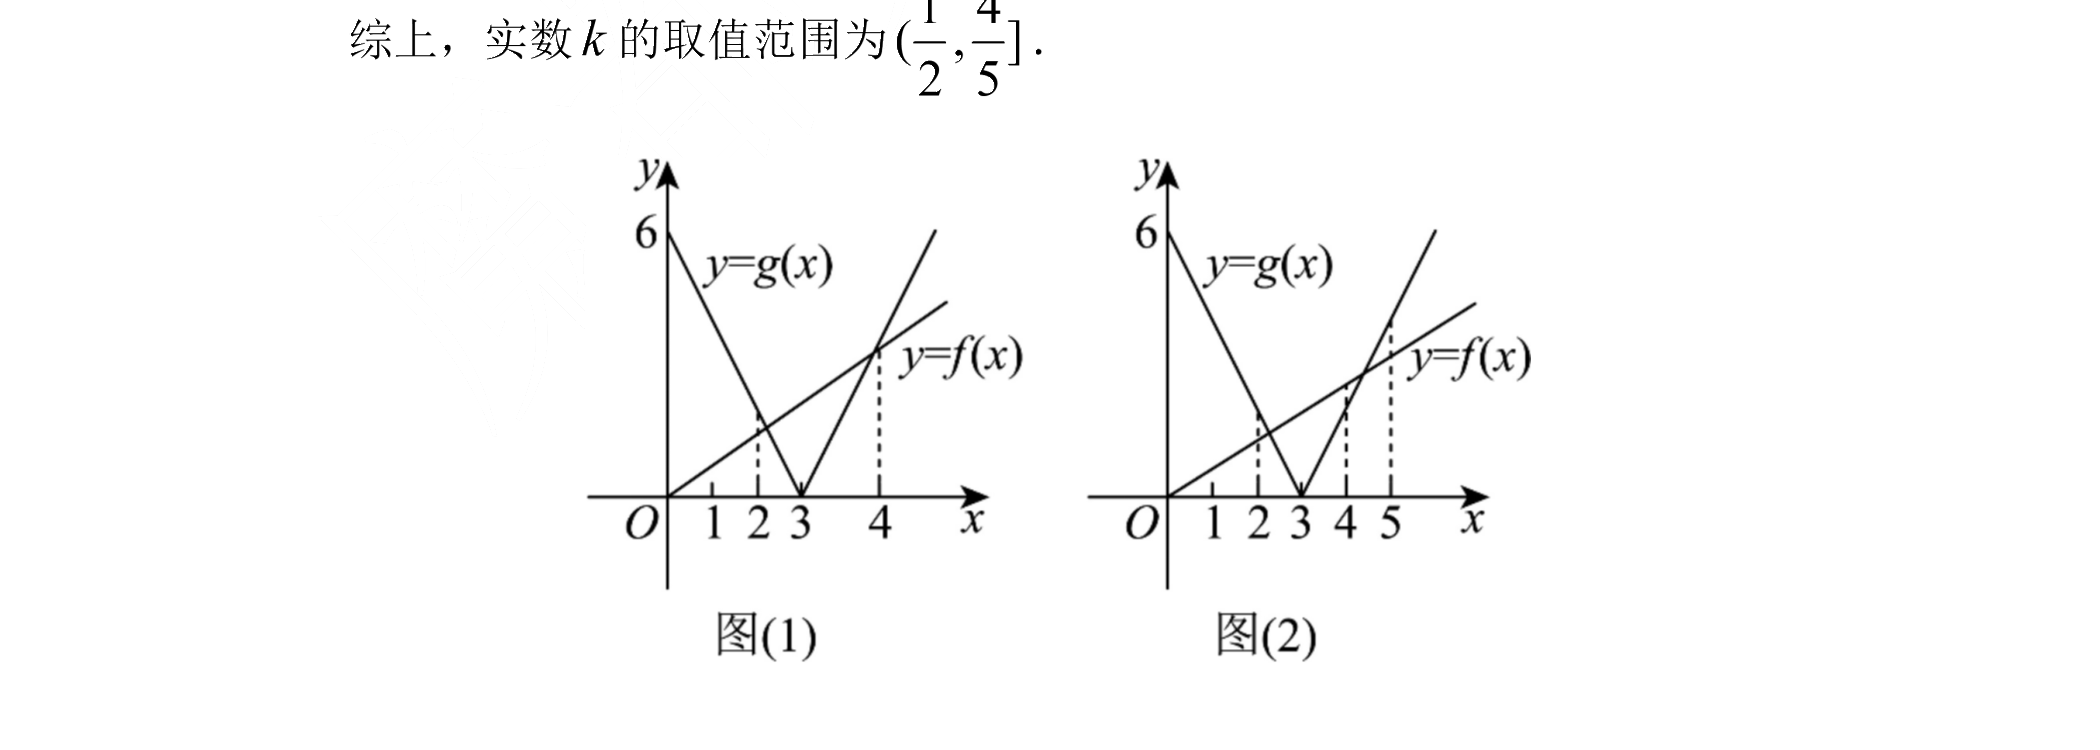
\includegraphics[width=0.72\textwidth]{figures/gao108_q11.png}
\end{center}

\step{综上，实数 $k$ 的取值范围为 $\left(\dfrac12,\dfrac45\right]$.}
\solend
\fi

\item 已知集合 $A=[1,a]\cup[a^3,a^4]$，集合 $B=\{x\mid x=x_1-x_2$，其中 $x_1$,$x_2\in A\}$. 若集合 $B$ 表
示的区间为一个闭区间，则实数 $a$ 的取值范围为\blankline[4.4em].

\ifanswer
\solbegin
\step{由题意得 $a^3>a>1$，则 $x_1-x_2$ 的最小值为 $1-a^4$，最大值为 $a^4-1$,}
\step{所以 $B=[1-a^4,a^4-1]$,}
\step{又因为 $a^4-a^3-(a-1)=a^3(a-1)-(a-1)=(a^3-1)(a-1)>0$,}
\step{所以 $a^4-a^3>a-1$，又集合 $B$ 表示的区间为一个闭区间,}
\step{则 $a^3-a\leqslant a^4-a^3$，化简得 $a^2-a-1\geqslant0$，又 $a>1$，解得 $a\geqslant\dfrac{1+\sqrt5}2$.}
\solend
\fi

\end{enumerate}

\bigsec{二、选择题}

\begin{enumerate}
\setcounter{enumi}{12}

\item 若 $a,b,c\in\R$，则下列不等式恒成立的是\mbox{（\quad）}% 原卷把答案“C”印在题干括号内、无【解析】

\keepwithprev
A. $\dfrac1a<\dfrac1b$\qquad B. $a^2<b^2$\qquad C. $\dfrac{a}{c^2+1}>\dfrac{b}{c^2+1}$\qquad D. $a\lvert c\rvert>b\lvert c\rvert$

\ifanswer
\ans{$C$}
\fi

\item 以下几个关系中正确的是\mbox{（\quad）}

\keepwithprev
A. $0\in\varnothing$\qquad\qquad\qquad B. $\varnothing\in\{x\mid x^2+1=0\}$

C. $\varnothing\subset\{0\}$\qquad\qquad\qquad D. $(A\cap B)\subset(A\cup B)$

\ifanswer
\solbegin
\step{$A$ 选项，$\varnothing$ 不包含任何元素，所以 $0\in\varnothing$ 错误，$A$ 错,}
\step{$B$ 选项，集合与集合之间关系不可以用 $\in$，$B$ 错,}
\step{$C$ 选项，空集是非空集合的真子集，所以 $\varnothing\subset\{0\}$ 正确，$C$ 对,}
\step{$D$ 选项，当 $A=B$ 时，$(A\cap B)=(A\cup B)$，$D$ 错,}
\step{故选 $C$.}
\solend
\fi

\item 设全集为 $U$，图中阴影部分所表示的集合是\mbox{（\quad）}% 原卷把答案“A”印在题干括号内、无【解析】

\keepwithprev
A. $B\cap\overline{A\cup C}$\qquad\qquad B. $(A\cup B)\cap(B\cup C)$

C. $(A\cup C)\cap\overline B$\qquad\qquad D. $(\overline A\cup\overline C)\cap B$

\ifanswer
\ans{$A$}
\fi

\item 对于 $k=0,1,2,\cdots$，定义集合 $A_k=\{20+k,26+2k\}$，并记 $S_k=A_0\cup A_1\cup\cdots\cup A_k$，则
使得集合 $S_n$ 中完全平方数的个数为奇数的最小正整数 $n$ 为\mbox{（\quad）}

\keepwithprev
A. $18$\qquad\qquad B. $19$\qquad\qquad C. $20$\qquad\qquad D. $21$

\ifanswer
\solbegin
\step{当 $k=0$ 时，$A_0=\{20,26\}$，对于 $k=0,1,2,\cdots$,}
\step{集合 $A_k$ 中最小的元素 $20>4^2$，若 $S_n$ 中完全平方数的个数为奇数，则 $n>4$,}
\step{（1）$20+k=5^2$ 时，$k=5$，$A_5=\{25,36\}$，此时 $S_5$ 中完全平方数为 $5^2$、$6^2$,}
\step{个数为 2;}
\step{$20+k=6^2$ 时，$k=16$，$A_{16}=\{36,58\}$，此时 $S_{16}$ 中完全平方数为 $5^2$、$6^2$,}
\step{个数为 2;}
\step{$20+k=7^2$ 时，$k=29$，$A_{29}=\{49,84\}$,}
\step{此时 $S_{29}$ 中完全平方数为 $5^2$、$6^2$、$7^2$、$8^2$，个数为 4;}
\step{$20+k=8^2$ 时，$k=44$，$A_{44}=\{64,114\}$,}
\step{此时 $S_{44}$ 中完全平方数为 $5^2$、$6^2$、$7^2$、$8^2$、$10^2$，个数为 5;}
\step{（2）因为 $k=0,1,2,\cdots,26+2k$ 一定为偶数,}
\step{所以 $26+2k=6^2$ 时，$k=5$，由上述分析得 $S_5$ 中完全平方数个数为 2;}
\step{$26+2k=8^2$ 时，$k=19$，$A_{19}=\{39,64\}$,}
\step{此时 $S_{19}$ 中完全平方数为 $5^2$、$6^2$、$8^2$，个数为 3.}
\step{综上，使集合 $S_n$ 中完全平方数的个数为奇数的最小正整数 $n=19$. 故选 $B$.}
\solend
\fi

\end{enumerate}

\bigsec{三、解答题}

\begin{enumerate}
\setcounter{enumi}{16}

\item 设全集 $U=\R$，集合 $A=\left\{x\,\middle|\,\dfrac{x-2}{x+2}\leqslant0\right\}$，$B=\{x\mid a\leqslant x<2a+1,a\in\R\}$，
$C=\{x\mid\lvert2x-1\rvert<5\}$.

（1）求集合 $A$、$\overline A\cup C$；

（2）若 $B\subseteq A$，求实数 $a$ 的取值范围.

\ifanswer
\solbegin
\ansspace*
\step{（1）不等式 $\dfrac{x-2}{x+2}\leqslant0$，等价于
$\begin{cases}(x-2)(x+2)\leqslant0\\x+2\neq0\end{cases}$，
解得 $\{x\mid-2<x\leqslant2\}$,}
\step{所以 $A=\{x\mid-2<x\leqslant2\}$，则 $\overline A=\{x\mid x\leqslant-2$ 或 $x>2\}$,}
\step{因为 $C=\{x\mid\lvert2x-1\rvert<5\}=\{x\mid-2<x<3\}$，所以 $\overline A\cup C=\R$；}
\step{（2）因为 $B\subseteq A$,}
\step{若 $B=\varnothing$，则 $a\geqslant2a+1$，解得 $a\leqslant-1$,}
\step{若 $B\neq\varnothing$，则
$\begin{cases}a<2a+1\\a>-2\\2a+1\leqslant2\end{cases}$，
解得 $-1<a\leqslant\dfrac12$,}
\step{综上所述，实数 $a$ 的取值范围为 $\left\{a\,\middle|\,a\leqslant\dfrac12\right\}$.}
\solend
\fi

\item 设 $a$、$b$、$c$、$d$ 是四个正数.

（1）已知 $a>b$，比较 $\dfrac{2a+b}{a+2b}$ 与 $\dfrac ab$ 的值的大小；

（2）若 $(1+a)(1+b)(1+c)(1+d)<16$，求证：$a$、$b$、$c$、$d$ 中至少有一个小于 1.

\ifanswer
\solbegin
\step{（1）$\dfrac{2a+b}{a+2b}-\dfrac ab=\dfrac{b^2-a^2}{b(a+2b)}<0$，所以 $\dfrac{2a+b}{a+2b}<\dfrac ab$.}
\step{（2）假设 $a$、$b$、$c$、$d$ 都不小于 1，即 $a$、$b$、$c$、$d$ 均大于等于 1,}
\step{即 $a\geqslant1$，$b\geqslant1$，$c\geqslant1$，$d\geqslant1$,}
\step{由均值不等式得 $1+a\geqslant2\sqrt a$,$1+b\geqslant2\sqrt b$,$1+c\geqslant2\sqrt c$,$1+d\geqslant2\sqrt d$,}
\step{故 $(1+a)(1+b)(1+c)(1+d)\geqslant16\sqrt{abcd}\geqslant16$,}
\step{当且仅当 $a=b=c=d=1$ 时取等号,}
\step{这与 $(1+a)(1+b)(1+c)(1+d)<16$ 矛盾，故假设不成立，原命题成立.}
\solend
\fi

\item 已知 $m\in\R$，一个二次项系数为 1 的一元二次方程的两个不等实根分别为 $x_1$ 和 $x_2$，且
满足
$\begin{cases}x_1^2+x_2^2=2m^2-4\\x_1+x_2=m\end{cases}$.

（1）直接写出该一元二次方程；

（2）若 $(3x_1-x_2)(3x_2-x_1)\geqslant-1$，求 $m$ 的取值范围；

（3）若方程的两根 $x_1$ 和 $x_2$ 都大于 $-1$，求 $m$ 的取值范围.

\ifanswer
\solbegin
\step{（1）设这个一元二次方程为 $x^2+bx+c=0$,}
\step{由
$\begin{cases}x_1^2+x_2^2=2m^2-4\\x_1+x_2=m\end{cases}$,}
\step{得 $(x_1+x_2)^2=x_1^2+x_2^2+2x_1x_2=2m^2-4+2x_1x_2=m^2$，即 $x_1x_2=\dfrac{4-m^2}2$,}
\step{由韦达定理得 $x_1+x_2=-b=m$，即 $x_1x_2=c=\dfrac{4-m^2}2$,}
\step{所以一元二次方程为 $x^2-mx+\dfrac{4-m^2}2=0$.}
\step{（2）$(3x_1-x_2)(3x_2-x_1)=9x_1x_2-3x_1^2-3x_2^2+x_1x_2=10x_1x_2-3(x_1^2+x_2^2)\geqslant-1$,}
\step{结合已知及（1）得 $x_1^2+x_2^2=2m^2-4$,$x_1x_2=\dfrac{4-m^2}2$,}
\step{代入得 $10\times\dfrac{4-m^2}2-3(2m^2-4)=-11m^2+32\geqslant-1\Rightarrow m^2\leqslant3$}
\step{$\Rightarrow-\sqrt3\leqslant m\leqslant\sqrt3$,}
\step{又 $\Delta=m^2-4\times\dfrac{4-m^2}2=3m^2-8>0\Rightarrow m<-\dfrac{2\sqrt6}3$ 或 $m>\dfrac{2\sqrt6}3$,}
\step{所以 $m\in\left[-\sqrt3,-\dfrac{2\sqrt6}3\right)\cup\left(\dfrac{2\sqrt6}3,\sqrt3\right]$.}
\step{（3）若方程的两根 $x_1$ 和 $x_2$ 都大于 $-1$，则
$\begin{cases}\Delta>0\\x_1+x_2>-2\\(x_1+1)(x_2+1)>0\end{cases}$,}
\step{所以
$\begin{cases}\Delta=3m^2-8>0\\m>-2\\[2pt]\dfrac{4-m^2}2+m+1>0\end{cases}$，
解得 $m\in\left(1-\sqrt7,-\dfrac{2\sqrt6}3\right)\cup\left(\dfrac{2\sqrt6}3,1+\sqrt7\right)$.}
\solend
\fi

\item 已知不等式 $2\leqslant ax^2+bx+c\leqslant3$ 的解集为 $\{x\mid2\leqslant x\leqslant3\}$.

（1）若 $a>0$，求 $6b+5c$ 的值；

（2）若 $a>0$，且不等式 $ax^2+(b-3)x-c\leqslant0$ 有且仅有 9 个整数解，求 $a$ 的取值范围；

（3）若 $a<0$，对任意的 $x<0$，不等式 $(ax-4)(x^2+b+c+1)\geqslant0$ 恒成立，求 $a^2-b+c$
的取值集合.

\ifanswer
\solbegin
\ansspace*
\step{（1）$a>0$,}
\step{结合二次函数图象得不等式 $ax^2+bx+c\leqslant3$ 的解集为 $\{x\mid2\leqslant x\leqslant3\}$,}
\step{且不等式 $ax^2+bx+c\geqslant2$ 的解集为 $R$,}
\step{所以方程 $ax^2+bx+c-3=0$ 的两根分别为 2 和 3,}
\step{则
$\begin{cases}2+3=-\dfrac ba\\[2pt]2\times3=\dfrac{c-3}a\end{cases}$，
得 $b=-5a$，$c=6a+3$,}
\step{所以 $6b+5c=6\times(-5a)+5(6a+3)=15$.}
\step{（2）若 $a>0$，且不等式 $ax^2+(b-3)x-c\leqslant0$ 有且仅有 9 个整数解,}
\step{由（1）得 $b=-5a$，$c=6a+3$,}
\step{不等式 $ax^2+bx+c\geqslant2$ 可化为 $ax^2-5ax+6a+1\geqslant0$.}
\step{由（1）得不等式 $ax^2+bx+c\geqslant2$ 的解集为 $R$,}
\step{所以 $ax^2-5ax+6a+1\geqslant0$ 恒成立,}
\step{所以
$\begin{cases}a>0\\\Delta=25a^2-4a(6a+1)\leqslant0\end{cases}$，
即
$\begin{cases}a>0\\a^2-4a=a(a-4)\leqslant0\end{cases}$，}
\step{解得 $0<a\leqslant4$.}
\step{不等式 $ax^2+(b-3)x-c\leqslant0$ 等价于 $ax^2-(5a+3)x-(6a+3)\leqslant0$,}
\step{所以 $[ax-(6a+3)](x+1)\leqslant0$，得 $-1\leqslant x\leqslant6+\dfrac3a$,}
\step{所以 $7\leqslant6+\dfrac3a<8$，解得 $\dfrac32<a\leqslant3$.}
\step{综上，$a$ 的取值范围为 $\left(\dfrac32,3\right]$.}
\step{（3）因为 $a<0$,}
\step{同（1）分析，不等式 $ax^2+bx+c\geqslant2$ 的解集为 $\{x\mid2\leqslant x\leqslant3\}$,}
\step{$ax^2+bx+c\leqslant3$ 的解集为 $R$,}
\step{所以方程 $ax^2+bx+c-2=0$ 的两根分别为 2 和 3,}
\step{则
$\begin{cases}2+3=-\dfrac ba\\[2pt]2\times3=\dfrac{c-2}a\end{cases}$，
得 $b=-5a$，$c=6a+2$.}
\step{所以不等式 $ax^2+bx+c=ax^2-5ax+6a+2\leqslant3$ 的解集为 $R$,}
\step{则 $ax^2-5ax+6a-1\leqslant0$ 恒成立,}
\step{所以
$\begin{cases}a<0\\\Delta=25a^2-4a(6a-1)\leqslant0\end{cases}$，
即
$\begin{cases}a<0\\a^2+4a=a(a+4)\leqslant0\end{cases}$，}
\step{解得 $-4\leqslant a<0$.}
\step{所以对任意的 $x<0$，不等式 $(ax-4)(x^2+b+c+1)\geqslant0$ 恒成立}
\step{转化为对任意的 $x<0$，不等式 $(ax-4)(x^2+a+3)\geqslant0$ 恒成立.}
\step{方程 $(ax-4)(x^2+a+3)=0$ 的两个根为 $x=\dfrac4a<0$,}
\step{$x=\pm\sqrt{-a-3}$（$a<-3$ 时成立）,}
\step{因而仅当 $ax-4=0$ 与 $x^2+a+3=0$ 的负根重合时满足条件,}
\step{解得唯一解为 $a=-4$，所以 $a^2-b+c=a^2+11a+2=-26$,}
\step{所以 $a^2-b+c$ 的取值集合为 $\{-26\}$.}
\solend
\fi

\item 已知集合 $A=\{1,2,3,4,5,6,7,8\}$，$M=\{(x,y)\mid x\in A,y\in A\}$，从 $M$ 中选取 $n$ 个不同的
元素组成一个序列：$(x_1,y_1)$,$(x_2,y_2),\cdots,(x_n,y_n)$，其中 $(x_i,y_i)$ 称为该序列的第 $i$ 项
（$i=1,2,\cdots,n$），若该序列的相邻项 $(x_i,y_i)$,$(x_{i+1},y_{i+1})$ 满足：
\[\begin{cases}\lvert x_{i+1}-x_i\rvert=3\\\lvert y_{i+1}-y_i\rvert=4\end{cases}
\quad\text{或}\quad
\begin{cases}\lvert x_{i+1}-x_i\rvert=4\\\lvert y_{i+1}-y_i\rvert=3\end{cases}\]
（$i=1,2,\cdots,n-1$），则称该序列为“$\Delta-$序列”.

（1）若一个 $\Delta-$序列的第一项为 $(4,4)$，请直接写出它所有可能的第二项；

（2）定义集合 $A=\{1,2,3,4,5,6,7,8\}$ 的两个子集：外侧集 $S=\{1,2,7,8\}$，内侧集
$T=\{3,4,5,6\}$. 证明：若 $\Delta-$序列中某一项的坐标在区域 $S\times S$ 内（即横、纵坐标均属于
$S$），则它的下一项坐标必定在区域 $T\times T$ 内；

（3）证明：不存在一个恰好有 5 项的 $\Delta-$序列，使其第一项为 $(1,8)$，且第五项为
$(8,1)$.

\ifanswer
\solbegin
\ansspace*
\step{（1）由题意，第一项为 $(x_1,y_1)=(4,4)$,}
\step{对于第二项 $(x_2,y_2)$，其坐标必须在 1~8 之间.}
\step{若 $\lvert x_2-4\rvert=3$,$\lvert y_2-4\rvert=4$，则 $x_2\in\{1,7\}$,}
\step{且 $y_2\in\{8\}$（因为 $4-4=0$ 不在集合 $A$ 中）. 此时可能的点为 $(1,8)$,$(7,8)$.}
\step{若 $\lvert x_2-4\rvert=4$,$\lvert y_2-4\rvert=3$，则 $x_2\in\{8\}$，且 $y_2\in\{1,7\}$.}
\step{此时可能的点为 $(8,1)$,$(8,7)$.}
\step{所以它所有可能的第二项为 $(1,8)$,$(7,8)$,$(8,1)$,$(8,7)$.}
\step{（2）已知某一项 $(x_t,y_t)\in S\times S$，即 $x_t\in\{1,2,7,8\}$ 且 $y_t\in\{1,2,7,8\}$.}
\step{由规则得下一步坐标的变化量为 3 和 4，设 $a\in S$ 变化 3 或 4 后的结果 $a'$:}
\step{当 $a=1$ 时，$1+3=4\in T$,$1+4=5\in T$；}
\step{当 $a=2$ 时，$2+3=5\in T$,$2+4=6\in T$；}
\step{当 $a=7$ 时，$7-3=4\in T$,$7-4=3\in T$；}
\step{当 $a=8$ 时，$8-3=5\in T$,$8-4=4\in T$.}
\step{（注：由于超出 1~8 范围的越界坐标不符合.）}
\step{由此可见，无论 $a$ 是 $S$ 中的哪一个数，加上或减去 3 或 4 之后,}
\step{得到的新坐标必属于集合 $T$.}
\step{因为 $\Delta-$序列每走一步，横坐标和纵坐标必定同时发生 3 和 4 的变化,}
\step{所以新的横坐标 $x_{i+1}$ 必属于 $T$，新的纵坐标 $y_{i+1}$ 也必属于 $T$,}
\step{即下一项 $(x_{i+1},y_{i+1})$ 必定在区域 $T\times T$ 内. ………10 分原命题得证.% 得分行混入证明，照录
}
\step{（3）假设存在这样一个包含 5 项的 $\Delta-$序列:}
\step{$(x_1,y_1)$,$(x_2,y_2)$,$(x_3,y_3)$,$(x_4,y_4)$,$(x_5,y_5)$.}
\step{已知第一项为 $(1,8)$，第五项为 $(8,1)$. 第 2 项必须是第 1 项 $(1,8)$ 的相邻点.}
\step{我们来找 $(1,8)$ 的相邻点：第 2 项只能是 $(4,4)$ 或 $(5,5)$,}
\step{第 4 项必须是第 5 项 $(8,1)$ 的相邻点（因为跳跃是双向可逆的）.}
\step{同理可算得，$(8,1)$ 的相邻点也只有两个：$(4,4)$ 和 $(5,5)$,}
\step{题目题干中明确规定，$\Delta-$序列由 $n$ 个不同的有序数对构成.% “题目题干”措辞重复，照录
}
\step{所以，第 2 项和第 4 项不能是同一个点. 这就意味着:}
\step{如果第 2 项是 $(4,4)$，第 4 项就必须是 $(5,5)$；反之亦然.}
\step{则第 3 项必须是 $(4,4)$ 和 $(5,5)$ 的公共相邻点.}
\step{$(4,4)$ 的相邻点集合为：$\{(1,8),(7,8),(8,1),(8,7)\}$,}
\step{$(5,5)$ 的相邻点集合为：$\{(2,1),(8,1),(1,2),(1,8)\}$,}
\step{所以，第 3 项只能填 $(1,8)$ 或者 $(8,1)$.}
\step{这与“序列由不同的有序数对构成”这一条件产生矛盾！}
\step{所以，不存在一个恰好有 5 项的 $\Delta-$序列,}
\step{使其第一项为 $(1,8)$，且第五项为 $(8,1)$.}
\solend
\fi

\end{enumerate}

\end{document}
"
%
% 原始材料：微信公众号“魔都数学加油站”文章，作者破晓，2026-11-03 17:19 发布；
% 连载“27学年高一108”，原文标题“27学年高一108——2026-2027年上海市五校联考高一上10月月考”；
% 原文链接：https://mp.weixin.qq.com/s/3nkP789Qar93NGMZXFFCSw。
% 正文为 14 张 PNG 页（第 2、3、6—13 页 4762×6735，第 1、4、5、14 页 2560×3620），
% 题目下印有【解析】，为讲评版。
% 题目、解析均据原图转录；卷面水印及公众号页脚未录入。
% 第 6 题解析的文氏图与第 11 题法二解析的两幅图象（图(1)、图(2)）裁自原图、去粉色水印
% 转灰度（gao108_q6.png、gao108_q11.png），第 6 题图属解析（仅答案版）、
% 第 11 题图属解析（仅答案版）。
%
% 卷首标题：原卷印作“2026-2027 年五校联考高一上 10 月月考”，标题下另印一行参与学校
% 名单“闵行中学、嘉定一中、松江一中、金山中学、嘉一实高”（全稿第 5 份原卷自印副标题，
% 按 14／24／49／50 成例照录，并登记进计数核对.py 的 SELFSUB）。
%
% 与原卷的排版差异：
%   ① 原文从第 3 题起，填空题编号为 3—12、选择题为 13—16、解答题为 17—21，本稿保留原题号；
%   ② 原卷每题下直接印【解析】，本稿按全稿惯例将解析置于答案版；第 4 题只印【答案】，
%      第 13、15 两题把答案印在题干括号内且无【解析】，均另提 \ans{}；
%   ③ 原卷副标题照录（见上）；
%   ④ 原卷填空横线按全稿惯例排为 \blankline[4.4em]；解答题按惯例加 \ansspace；选择题括号排
%      \mbox{（\quad）}、选项段前按惯例加 \keepwithprev；
%   ⑤ 原卷数集排斜体 $R$／$N$，按全稿惯例改 \R、\N。
%
% 原卷红色强调照录为黑体：第 11 题解析的“法一：”“法二：”原卷排红色，按 53 成例排
% \stepm{法一：}／\stepm{法二：}（加粗着色）。
%
% 原卷存疑：第 10 题题干“变项和”定义中“将 $M$ 中每个元素 $m$ 都乘以 $(-1)^n$ 后再求和”
% 的 $n$ 未加界定（据解析应为该元素在 $\{1,2,\cdots,2026\}$ 中的序号），照录。
% 第 21 题 (2) 解析末行“即下一项 $(x_{i+1},y_{i+1})$ 必定在区域 $T\times T$ 内. ………10 分
% 原命题得证.”，原卷把得分点行混入证明（“原命题”按上下文为“原命题的逆否”），照录。
% 第 21 题 (3) 解析“题目题干中明确规定”，“题目题干”措辞重复，照录。
%
% 行数核对：逐题数 \step/\stepm 条数，合计 164 条（Q3：3；Q4：0；Q5：2；Q6：1；Q7：3；
% Q8：3；Q9：3；Q10：6；Q11：21；Q12：5；Q13：0；Q14：5；Q15：0；Q16：15；Q17：7；
% Q18：7；Q19：13；Q20：34；Q21：36），与原卷印刷行逐题相等。第 4 题只印【答案】、
% 第 13、15 题括号内印答案，均提 \ans{}，不计入 \step 账。
%
\documentclass[a4paper,11pt]{article}
\usepackage{common}

\begin{document}

\examtitlest[3]{2026--2027 年五校联考高一上 10 月月考}{闵行中学、嘉定一中、松江一中、金山中学、嘉一实高}

\bigsec{一、填空题}

\begin{enumerate}
\setcounter{enumi}{2}

\item 已知等式 $2x^2+3x+5=2ax^2+a(3x+1)+c$ 恒成立，则实数 $a+c$ 的值为\blankline[4.4em].

\ifanswer
\solbegin
\step{因为 $2x^2+3x+5=2ax^2+a(3x+1)+c$ 恒成立,}
\step{即 $2x^2+3x+5=2ax^2+3ax+(a+c)$ 恒成立，所以
$\begin{cases}2=2a\\3=3a\\5=a+c\end{cases}$,}
\step{所以 $a+c=5$.}
\solend
\fi

\item 不等式 $\dfrac1x<\dfrac12$ 的解集是\blankline[4.4em].

\ifanswer
\ans{$(-\infty,0)\cup(2,+\infty)$}
\fi

\item 已知 $a$、$b$ 都是实数，则“$a^2=b^2$”是“$a^2+b^2=2ab$”的\blankline[4.4em]条件.

\ifanswer
\solbegin
\step{$a^2=b^2$ 等价于 $a=\pm b$；$a^2+b^2=2ab$ 等价于 $(a-b)^2=0$ 等价于 $a=b$,}
\step{故“$a^2=b^2$”是“$a^2+b^2=2ab$”的必要不充分条件.}
\solend
\fi

\item 已知全集 $U=\{x\mid x$ 为不大于 20 的素数$\}$，$A\cap\overline B=\{5\}$，$\overline A\cap B=\{3\}$，
$\overline{A\cup B}=\{7,13,17,19\}$，则 $A=$\blankline[4.4em].

\ifanswer
\solbegin
\step{如图所示，$A=\{2,5,11\}$.}

\begin{center}
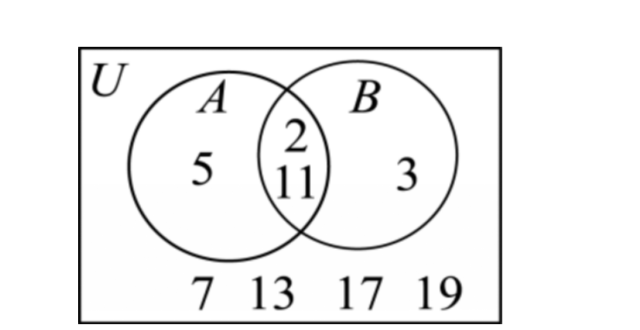
\includegraphics[width=0.24\textwidth]{figures/gao108_q6.png}
\end{center}

\solend
\fi

\item 若 $x\in A$，则 $\dfrac1x\in A$，就称 $A$ 自倒集合，集合 $M=\left\{-2,-1,0,\dfrac12,\dfrac13,1,2,3,4\right\}$ 的所有非空
子集中，自倒集合的个数为\blankline[4.4em].

\ifanswer
\solbegin
\step{由新定义，集合 $M$ 中的元素 1 和 $-1$ 倒数等于本身，2 和 $\dfrac12$，3 和 $\dfrac13$ 互为倒数,}
\step{故满足条件的自倒集合与集合 $\{-1,1,2,3\}$ 的非空子集的个数相同,}
\step{则其个数为 $2^4-1=15$.}
\solend
\fi

\item 设集合 $M=\{(x,y)\mid y=x^2+2bx+1\}$，$N=\{(x,y)\mid y=x+b\}(b\in\R)$，若
$M\cap N=\varnothing$，则实数 $b$ 的取值范围为\blankline[4.4em].

\ifanswer
\solbegin
\step{因为 $M\cap N=\varnothing$，所以
$\begin{cases}y=x^2+2bx+1\\y=x+b\end{cases}$
无解，则 $x^2+(2b-1)x+(1-b)=0$,}
\step{则 $\triangle=(2b-1)^2-4\times1\times(1-b)=4b^2-3<0$，解得 $-\dfrac{\sqrt3}2<b<\dfrac{\sqrt3}2$,}
\step{即实数 $b$ 的取值范围为 $\left(-\dfrac{\sqrt3}2,\dfrac{\sqrt3}2\right)$.}
\solend
\fi

\item 已知集合 $A=\left\{x\,\middle|\,\dfrac{x-a}{x^2-1}=1\right\}$ 有唯一元素，用列举法表示满足集合 $A$ 的条件的 $a$ 的取值集
合\blankline[4.4em].

\ifanswer
\solbegin
\step{$a=1$,$\dfrac{1}{x+1}=1$，一解；$a=-1$,$\dfrac{1}{x-1}=1$，一解；}
\step{$x-a=x^2-1$，一解时，$a=\dfrac54$,}
\step{综上，$a$ 的取值集合为 $\left\{-1,1,\dfrac54\right\}$.}
\solend
\fi

\item 已知集合 $M$ 的元素均为正整数，定义集合 $M$ 的“变项和”为：将 $M$ 中每个元素 $m$ 都乘
以 $(-1)^n$ 后再求和. 若集合 $A=\{n\mid1\leqslant n\leqslant2026,n\in\N\}$，则集合 $A$ 的所有非空子集的“变
项和”的总和为\blankline[4.4em].% $n$ 未加界定（据解析为元素序号），照录

\ifanswer
\solbegin
\step{$A=\{n\mid1\leqslant n\leqslant2026,n\in\N\}=\{1,2,\cdots,2026\}$,}
\step{1 在所有非空子集中共出现 $C_{2025}^{0}+C_{2025}^{1}+\cdots+C_{2025}^{2025}=2^{2025}$ 次,}
\step{同理 $2,3,\cdots,2026$ 都出现 $2^{2025}$ 次,}
\step{则集合 $A$ 的所有非空子集的“变项和”的总和}
\step{为 $2^{2025}\times[1\times(-1)^1+2\times(-1)^2+\cdots+2026\times(-1)^{2026}]$}
\step{$=2^{2025}\times(-1+2-3+4-\cdots-2025+2026)=1013\times2^{2025}$.}
\solend
\fi

\item 已知 $0<k<2$，定义 $[x]$ 为不超过 $x$ 的最大整数，区间 $[a,b]$（或 $(a,b)$，$[a,b)$，
$(a,b]$）的长度记为 $b-a$. 若关于 $x$ 的不等式 $k[x]>\lvert2[x]-6\rvert$ 的解集对应区间的长度为 $2$，
则 $k$ 的取值范围是\blankline[4.4em].

\ifanswer
\solbegin
\stepm{法一：}{由题意得 $\lvert2[x]-6\rvert=
\begin{cases}2[x]-6,x\geqslant3\\-2[x]+6,x<3\end{cases}$.}
\step{①当 $x\geqslant3$ 时，不等式 $k[x]>\lvert2[x]-6\rvert$ 可化为 $k[x]>2[x]-6$,}
\step{即 $(2-k)[x]<6$,}
\step{当 $0<k<2$ 时，解不等式 $(2-k)[x]<6$ 得 $[x]<\dfrac6{2-k}$.}
\step{②当 $x<3$ 时，不等式 $k[x]>\lvert2[x]-6\rvert$ 可化为 $k[x]>-2[x]+6$,}
\step{即 $(k+2)[x]>6$.}
\step{当 $0<k<2$ 时，解不等式 $(k+2)[x]>6$ 得 $[x]>\dfrac6{k+2}$.}
\step{综上所述，不等式 $k[x]>\lvert2[x]-6\rvert$ 的解集需满足 $\dfrac6{k+2}<[x]<\dfrac6{2-k}$,}
\step{由题意得在区间 $\left[\dfrac6{k+2},\dfrac6{2-k}\right]$ 内有两个整数,}
\step{由于 $\dfrac6{k+2}\in\left(\dfrac32,3\right)$，所以 $\dfrac6{2-k}\leqslant5$，得 $k\leqslant\dfrac45$.}
\step{因此 $k\in\left(0,\dfrac45\right]$，得 $\dfrac6{k+2}\in\left[\dfrac75,3\right)$，$\dfrac6{2-k}\in(3,5]$,}
\step{区间 $\left[\dfrac6{k+2},\dfrac6{2-k}\right]$ 内的两个整数是 3、4，所以 $4<\dfrac6{2-k}\leqslant5$，解得 $\dfrac12<k\leqslant\dfrac45$,}
\step{即 $k\in\left(\dfrac12,\dfrac45\right]$.}
\stepm{法二：}{令 $f(x)=kx$，$g(x)=\lvert2x-6\rvert$，画出 $g(x)$、$f(x)$ 的图象,}
\step{由于不等式 $k[x]>\lvert2[x]-6\rvert$ 的解集对应区间的长度为 2,}
\step{因此解集只可能为 $[3,5)$ 或 $[2,4)$.}
\step{当解集为 $[3,5)$ 时，如图（2），数形结合易得
$\begin{cases}f(2)\leqslant g(2)\\f(4)>g(4)\\f(5)\leqslant g(5)\end{cases}$,}
\step{即
$\begin{cases}2k\leqslant\lvert2\times2-6\rvert\\4k>\lvert2\times4-6\rvert\\5k\leqslant\lvert2\times5-6\rvert\end{cases}$，
解得
$\begin{cases}k\leqslant1\\k>\dfrac12\\k\leqslant\dfrac45\end{cases}$，
所以 $\dfrac12<k\leqslant\dfrac45$，满足 $0<k<2$,}
\step{当解集为 $[2,4)$ 时，如图（1），数形结合易得
$\begin{cases}f(2)>g(2)\\f(4)\leqslant g(4)\end{cases}$,}
\step{即
$\begin{cases}2k>\lvert2\times2-6\rvert\\4k\leqslant\lvert2\times4-6\rvert\end{cases}$，
无解.}

\begin{center}
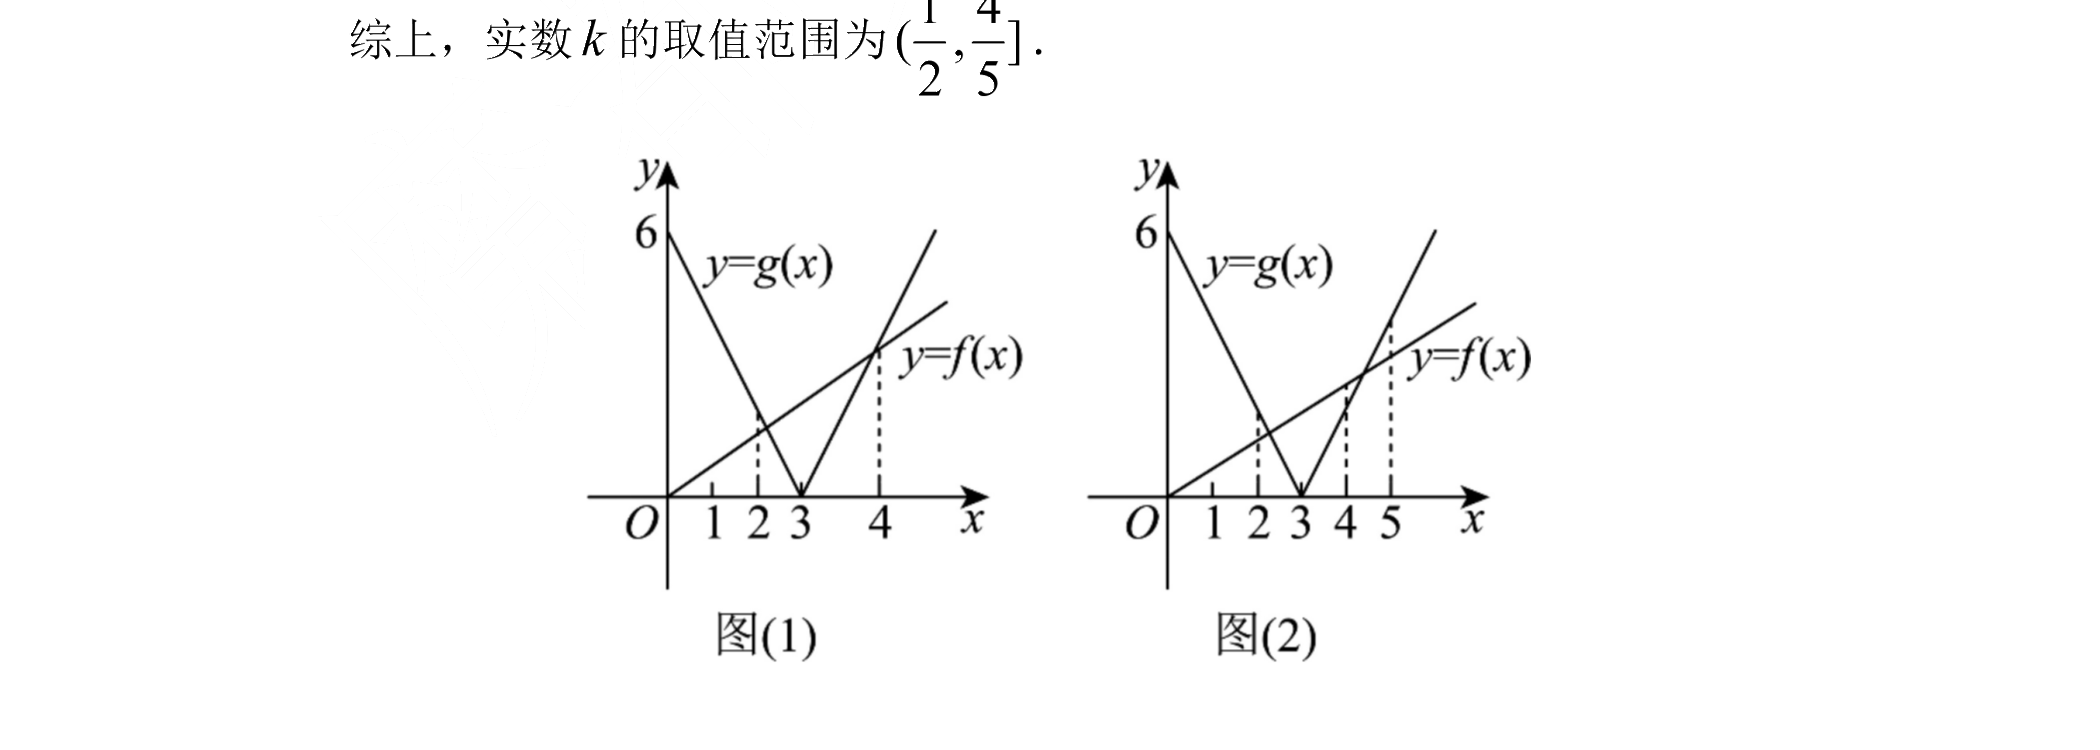
\includegraphics[width=0.72\textwidth]{figures/gao108_q11.png}
\end{center}

\step{综上，实数 $k$ 的取值范围为 $\left(\dfrac12,\dfrac45\right]$.}
\solend
\fi

\item 已知集合 $A=[1,a]\cup[a^3,a^4]$，集合 $B=\{x\mid x=x_1-x_2$，其中 $x_1$,$x_2\in A\}$. 若集合 $B$ 表
示的区间为一个闭区间，则实数 $a$ 的取值范围为\blankline[4.4em].

\ifanswer
\solbegin
\step{由题意得 $a^3>a>1$，则 $x_1-x_2$ 的最小值为 $1-a^4$，最大值为 $a^4-1$,}
\step{所以 $B=[1-a^4,a^4-1]$,}
\step{又因为 $a^4-a^3-(a-1)=a^3(a-1)-(a-1)=(a^3-1)(a-1)>0$,}
\step{所以 $a^4-a^3>a-1$，又集合 $B$ 表示的区间为一个闭区间,}
\step{则 $a^3-a\leqslant a^4-a^3$，化简得 $a^2-a-1\geqslant0$，又 $a>1$，解得 $a\geqslant\dfrac{1+\sqrt5}2$.}
\solend
\fi

\end{enumerate}

\bigsec{二、选择题}

\begin{enumerate}
\setcounter{enumi}{12}

\item 若 $a,b,c\in\R$，则下列不等式恒成立的是\mbox{（\quad）}% 原卷把答案“C”印在题干括号内、无【解析】

\keepwithprev
A. $\dfrac1a<\dfrac1b$\qquad B. $a^2<b^2$\qquad C. $\dfrac{a}{c^2+1}>\dfrac{b}{c^2+1}$\qquad D. $a\lvert c\rvert>b\lvert c\rvert$

\ifanswer
\ans{$C$}
\fi

\item 以下几个关系中正确的是\mbox{（\quad）}

\keepwithprev
A. $0\in\varnothing$\qquad\qquad\qquad B. $\varnothing\in\{x\mid x^2+1=0\}$

C. $\varnothing\subset\{0\}$\qquad\qquad\qquad D. $(A\cap B)\subset(A\cup B)$

\ifanswer
\solbegin
\step{$A$ 选项，$\varnothing$ 不包含任何元素，所以 $0\in\varnothing$ 错误，$A$ 错,}
\step{$B$ 选项，集合与集合之间关系不可以用 $\in$，$B$ 错,}
\step{$C$ 选项，空集是非空集合的真子集，所以 $\varnothing\subset\{0\}$ 正确，$C$ 对,}
\step{$D$ 选项，当 $A=B$ 时，$(A\cap B)=(A\cup B)$，$D$ 错,}
\step{故选 $C$.}
\solend
\fi

\item 设全集为 $U$，图中阴影部分所表示的集合是\mbox{（\quad）}% 原卷把答案“A”印在题干括号内、无【解析】

\keepwithprev
A. $B\cap\overline{A\cup C}$\qquad\qquad B. $(A\cup B)\cap(B\cup C)$

C. $(A\cup C)\cap\overline B$\qquad\qquad D. $(\overline A\cup\overline C)\cap B$

\ifanswer
\ans{$A$}
\fi

\item 对于 $k=0,1,2,\cdots$，定义集合 $A_k=\{20+k,26+2k\}$，并记 $S_k=A_0\cup A_1\cup\cdots\cup A_k$，则
使得集合 $S_n$ 中完全平方数的个数为奇数的最小正整数 $n$ 为\mbox{（\quad）}

\keepwithprev
A. $18$\qquad\qquad B. $19$\qquad\qquad C. $20$\qquad\qquad D. $21$

\ifanswer
\solbegin
\step{当 $k=0$ 时，$A_0=\{20,26\}$，对于 $k=0,1,2,\cdots$,}
\step{集合 $A_k$ 中最小的元素 $20>4^2$，若 $S_n$ 中完全平方数的个数为奇数，则 $n>4$,}
\step{（1）$20+k=5^2$ 时，$k=5$，$A_5=\{25,36\}$，此时 $S_5$ 中完全平方数为 $5^2$、$6^2$,}
\step{个数为 2;}
\step{$20+k=6^2$ 时，$k=16$，$A_{16}=\{36,58\}$，此时 $S_{16}$ 中完全平方数为 $5^2$、$6^2$,}
\step{个数为 2;}
\step{$20+k=7^2$ 时，$k=29$，$A_{29}=\{49,84\}$,}
\step{此时 $S_{29}$ 中完全平方数为 $5^2$、$6^2$、$7^2$、$8^2$，个数为 4;}
\step{$20+k=8^2$ 时，$k=44$，$A_{44}=\{64,114\}$,}
\step{此时 $S_{44}$ 中完全平方数为 $5^2$、$6^2$、$7^2$、$8^2$、$10^2$，个数为 5;}
\step{（2）因为 $k=0,1,2,\cdots,26+2k$ 一定为偶数,}
\step{所以 $26+2k=6^2$ 时，$k=5$，由上述分析得 $S_5$ 中完全平方数个数为 2;}
\step{$26+2k=8^2$ 时，$k=19$，$A_{19}=\{39,64\}$,}
\step{此时 $S_{19}$ 中完全平方数为 $5^2$、$6^2$、$8^2$，个数为 3.}
\step{综上，使集合 $S_n$ 中完全平方数的个数为奇数的最小正整数 $n=19$. 故选 $B$.}
\solend
\fi

\end{enumerate}

\bigsec{三、解答题}

\begin{enumerate}
\setcounter{enumi}{16}

\item 设全集 $U=\R$，集合 $A=\left\{x\,\middle|\,\dfrac{x-2}{x+2}\leqslant0\right\}$，$B=\{x\mid a\leqslant x<2a+1,a\in\R\}$，
$C=\{x\mid\lvert2x-1\rvert<5\}$.

（1）求集合 $A$、$\overline A\cup C$；

（2）若 $B\subseteq A$，求实数 $a$ 的取值范围.

\ifanswer
\solbegin
\ansspace*
\step{（1）不等式 $\dfrac{x-2}{x+2}\leqslant0$，等价于
$\begin{cases}(x-2)(x+2)\leqslant0\\x+2\neq0\end{cases}$，
解得 $\{x\mid-2<x\leqslant2\}$,}
\step{所以 $A=\{x\mid-2<x\leqslant2\}$，则 $\overline A=\{x\mid x\leqslant-2$ 或 $x>2\}$,}
\step{因为 $C=\{x\mid\lvert2x-1\rvert<5\}=\{x\mid-2<x<3\}$，所以 $\overline A\cup C=\R$；}
\step{（2）因为 $B\subseteq A$,}
\step{若 $B=\varnothing$，则 $a\geqslant2a+1$，解得 $a\leqslant-1$,}
\step{若 $B\neq\varnothing$，则
$\begin{cases}a<2a+1\\a>-2\\2a+1\leqslant2\end{cases}$，
解得 $-1<a\leqslant\dfrac12$,}
\step{综上所述，实数 $a$ 的取值范围为 $\left\{a\,\middle|\,a\leqslant\dfrac12\right\}$.}
\solend
\fi

\item 设 $a$、$b$、$c$、$d$ 是四个正数.

（1）已知 $a>b$，比较 $\dfrac{2a+b}{a+2b}$ 与 $\dfrac ab$ 的值的大小；

（2）若 $(1+a)(1+b)(1+c)(1+d)<16$，求证：$a$、$b$、$c$、$d$ 中至少有一个小于 1.

\ifanswer
\solbegin
\step{（1）$\dfrac{2a+b}{a+2b}-\dfrac ab=\dfrac{b^2-a^2}{b(a+2b)}<0$，所以 $\dfrac{2a+b}{a+2b}<\dfrac ab$.}
\step{（2）假设 $a$、$b$、$c$、$d$ 都不小于 1，即 $a$、$b$、$c$、$d$ 均大于等于 1,}
\step{即 $a\geqslant1$，$b\geqslant1$，$c\geqslant1$，$d\geqslant1$,}
\step{由均值不等式得 $1+a\geqslant2\sqrt a$,$1+b\geqslant2\sqrt b$,$1+c\geqslant2\sqrt c$,$1+d\geqslant2\sqrt d$,}
\step{故 $(1+a)(1+b)(1+c)(1+d)\geqslant16\sqrt{abcd}\geqslant16$,}
\step{当且仅当 $a=b=c=d=1$ 时取等号,}
\step{这与 $(1+a)(1+b)(1+c)(1+d)<16$ 矛盾，故假设不成立，原命题成立.}
\solend
\fi

\item 已知 $m\in\R$，一个二次项系数为 1 的一元二次方程的两个不等实根分别为 $x_1$ 和 $x_2$，且
满足
$\begin{cases}x_1^2+x_2^2=2m^2-4\\x_1+x_2=m\end{cases}$.

（1）直接写出该一元二次方程；

（2）若 $(3x_1-x_2)(3x_2-x_1)\geqslant-1$，求 $m$ 的取值范围；

（3）若方程的两根 $x_1$ 和 $x_2$ 都大于 $-1$，求 $m$ 的取值范围.

\ifanswer
\solbegin
\step{（1）设这个一元二次方程为 $x^2+bx+c=0$,}
\step{由
$\begin{cases}x_1^2+x_2^2=2m^2-4\\x_1+x_2=m\end{cases}$,}
\step{得 $(x_1+x_2)^2=x_1^2+x_2^2+2x_1x_2=2m^2-4+2x_1x_2=m^2$，即 $x_1x_2=\dfrac{4-m^2}2$,}
\step{由韦达定理得 $x_1+x_2=-b=m$，即 $x_1x_2=c=\dfrac{4-m^2}2$,}
\step{所以一元二次方程为 $x^2-mx+\dfrac{4-m^2}2=0$.}
\step{（2）$(3x_1-x_2)(3x_2-x_1)=9x_1x_2-3x_1^2-3x_2^2+x_1x_2=10x_1x_2-3(x_1^2+x_2^2)\geqslant-1$,}
\step{结合已知及（1）得 $x_1^2+x_2^2=2m^2-4$,$x_1x_2=\dfrac{4-m^2}2$,}
\step{代入得 $10\times\dfrac{4-m^2}2-3(2m^2-4)=-11m^2+32\geqslant-1\Rightarrow m^2\leqslant3$}
\step{$\Rightarrow-\sqrt3\leqslant m\leqslant\sqrt3$,}
\step{又 $\Delta=m^2-4\times\dfrac{4-m^2}2=3m^2-8>0\Rightarrow m<-\dfrac{2\sqrt6}3$ 或 $m>\dfrac{2\sqrt6}3$,}
\step{所以 $m\in\left[-\sqrt3,-\dfrac{2\sqrt6}3\right)\cup\left(\dfrac{2\sqrt6}3,\sqrt3\right]$.}
\step{（3）若方程的两根 $x_1$ 和 $x_2$ 都大于 $-1$，则
$\begin{cases}\Delta>0\\x_1+x_2>-2\\(x_1+1)(x_2+1)>0\end{cases}$,}
\step{所以
$\begin{cases}\Delta=3m^2-8>0\\m>-2\\[2pt]\dfrac{4-m^2}2+m+1>0\end{cases}$，
解得 $m\in\left(1-\sqrt7,-\dfrac{2\sqrt6}3\right)\cup\left(\dfrac{2\sqrt6}3,1+\sqrt7\right)$.}
\solend
\fi

\item 已知不等式 $2\leqslant ax^2+bx+c\leqslant3$ 的解集为 $\{x\mid2\leqslant x\leqslant3\}$.

（1）若 $a>0$，求 $6b+5c$ 的值；

（2）若 $a>0$，且不等式 $ax^2+(b-3)x-c\leqslant0$ 有且仅有 9 个整数解，求 $a$ 的取值范围；

（3）若 $a<0$，对任意的 $x<0$，不等式 $(ax-4)(x^2+b+c+1)\geqslant0$ 恒成立，求 $a^2-b+c$
的取值集合.

\ifanswer
\solbegin
\ansspace*
\step{（1）$a>0$,}
\step{结合二次函数图象得不等式 $ax^2+bx+c\leqslant3$ 的解集为 $\{x\mid2\leqslant x\leqslant3\}$,}
\step{且不等式 $ax^2+bx+c\geqslant2$ 的解集为 $R$,}
\step{所以方程 $ax^2+bx+c-3=0$ 的两根分别为 2 和 3,}
\step{则
$\begin{cases}2+3=-\dfrac ba\\[2pt]2\times3=\dfrac{c-3}a\end{cases}$，
得 $b=-5a$，$c=6a+3$,}
\step{所以 $6b+5c=6\times(-5a)+5(6a+3)=15$.}
\step{（2）若 $a>0$，且不等式 $ax^2+(b-3)x-c\leqslant0$ 有且仅有 9 个整数解,}
\step{由（1）得 $b=-5a$，$c=6a+3$,}
\step{不等式 $ax^2+bx+c\geqslant2$ 可化为 $ax^2-5ax+6a+1\geqslant0$.}
\step{由（1）得不等式 $ax^2+bx+c\geqslant2$ 的解集为 $R$,}
\step{所以 $ax^2-5ax+6a+1\geqslant0$ 恒成立,}
\step{所以
$\begin{cases}a>0\\\Delta=25a^2-4a(6a+1)\leqslant0\end{cases}$，
即
$\begin{cases}a>0\\a^2-4a=a(a-4)\leqslant0\end{cases}$，}
\step{解得 $0<a\leqslant4$.}
\step{不等式 $ax^2+(b-3)x-c\leqslant0$ 等价于 $ax^2-(5a+3)x-(6a+3)\leqslant0$,}
\step{所以 $[ax-(6a+3)](x+1)\leqslant0$，得 $-1\leqslant x\leqslant6+\dfrac3a$,}
\step{所以 $7\leqslant6+\dfrac3a<8$，解得 $\dfrac32<a\leqslant3$.}
\step{综上，$a$ 的取值范围为 $\left(\dfrac32,3\right]$.}
\step{（3）因为 $a<0$,}
\step{同（1）分析，不等式 $ax^2+bx+c\geqslant2$ 的解集为 $\{x\mid2\leqslant x\leqslant3\}$,}
\step{$ax^2+bx+c\leqslant3$ 的解集为 $R$,}
\step{所以方程 $ax^2+bx+c-2=0$ 的两根分别为 2 和 3,}
\step{则
$\begin{cases}2+3=-\dfrac ba\\[2pt]2\times3=\dfrac{c-2}a\end{cases}$，
得 $b=-5a$，$c=6a+2$.}
\step{所以不等式 $ax^2+bx+c=ax^2-5ax+6a+2\leqslant3$ 的解集为 $R$,}
\step{则 $ax^2-5ax+6a-1\leqslant0$ 恒成立,}
\step{所以
$\begin{cases}a<0\\\Delta=25a^2-4a(6a-1)\leqslant0\end{cases}$，
即
$\begin{cases}a<0\\a^2+4a=a(a+4)\leqslant0\end{cases}$，}
\step{解得 $-4\leqslant a<0$.}
\step{所以对任意的 $x<0$，不等式 $(ax-4)(x^2+b+c+1)\geqslant0$ 恒成立}
\step{转化为对任意的 $x<0$，不等式 $(ax-4)(x^2+a+3)\geqslant0$ 恒成立.}
\step{方程 $(ax-4)(x^2+a+3)=0$ 的两个根为 $x=\dfrac4a<0$,}
\step{$x=\pm\sqrt{-a-3}$（$a<-3$ 时成立）,}
\step{因而仅当 $ax-4=0$ 与 $x^2+a+3=0$ 的负根重合时满足条件,}
\step{解得唯一解为 $a=-4$，所以 $a^2-b+c=a^2+11a+2=-26$,}
\step{所以 $a^2-b+c$ 的取值集合为 $\{-26\}$.}
\solend
\fi

\item 已知集合 $A=\{1,2,3,4,5,6,7,8\}$，$M=\{(x,y)\mid x\in A,y\in A\}$，从 $M$ 中选取 $n$ 个不同的
元素组成一个序列：$(x_1,y_1)$,$(x_2,y_2),\cdots,(x_n,y_n)$，其中 $(x_i,y_i)$ 称为该序列的第 $i$ 项
（$i=1,2,\cdots,n$），若该序列的相邻项 $(x_i,y_i)$,$(x_{i+1},y_{i+1})$ 满足：
\[\begin{cases}\lvert x_{i+1}-x_i\rvert=3\\\lvert y_{i+1}-y_i\rvert=4\end{cases}
\quad\text{或}\quad
\begin{cases}\lvert x_{i+1}-x_i\rvert=4\\\lvert y_{i+1}-y_i\rvert=3\end{cases}\]
（$i=1,2,\cdots,n-1$），则称该序列为“$\Delta-$序列”.

（1）若一个 $\Delta-$序列的第一项为 $(4,4)$，请直接写出它所有可能的第二项；

（2）定义集合 $A=\{1,2,3,4,5,6,7,8\}$ 的两个子集：外侧集 $S=\{1,2,7,8\}$，内侧集
$T=\{3,4,5,6\}$. 证明：若 $\Delta-$序列中某一项的坐标在区域 $S\times S$ 内（即横、纵坐标均属于
$S$），则它的下一项坐标必定在区域 $T\times T$ 内；

（3）证明：不存在一个恰好有 5 项的 $\Delta-$序列，使其第一项为 $(1,8)$，且第五项为
$(8,1)$.

\ifanswer
\solbegin
\ansspace*
\step{（1）由题意，第一项为 $(x_1,y_1)=(4,4)$,}
\step{对于第二项 $(x_2,y_2)$，其坐标必须在 1~8 之间.}
\step{若 $\lvert x_2-4\rvert=3$,$\lvert y_2-4\rvert=4$，则 $x_2\in\{1,7\}$,}
\step{且 $y_2\in\{8\}$（因为 $4-4=0$ 不在集合 $A$ 中）. 此时可能的点为 $(1,8)$,$(7,8)$.}
\step{若 $\lvert x_2-4\rvert=4$,$\lvert y_2-4\rvert=3$，则 $x_2\in\{8\}$，且 $y_2\in\{1,7\}$.}
\step{此时可能的点为 $(8,1)$,$(8,7)$.}
\step{所以它所有可能的第二项为 $(1,8)$,$(7,8)$,$(8,1)$,$(8,7)$.}
\step{（2）已知某一项 $(x_t,y_t)\in S\times S$，即 $x_t\in\{1,2,7,8\}$ 且 $y_t\in\{1,2,7,8\}$.}
\step{由规则得下一步坐标的变化量为 3 和 4，设 $a\in S$ 变化 3 或 4 后的结果 $a'$:}
\step{当 $a=1$ 时，$1+3=4\in T$,$1+4=5\in T$；}
\step{当 $a=2$ 时，$2+3=5\in T$,$2+4=6\in T$；}
\step{当 $a=7$ 时，$7-3=4\in T$,$7-4=3\in T$；}
\step{当 $a=8$ 时，$8-3=5\in T$,$8-4=4\in T$.}
\step{（注：由于超出 1~8 范围的越界坐标不符合.）}
\step{由此可见，无论 $a$ 是 $S$ 中的哪一个数，加上或减去 3 或 4 之后,}
\step{得到的新坐标必属于集合 $T$.}
\step{因为 $\Delta-$序列每走一步，横坐标和纵坐标必定同时发生 3 和 4 的变化,}
\step{所以新的横坐标 $x_{i+1}$ 必属于 $T$，新的纵坐标 $y_{i+1}$ 也必属于 $T$,}
\step{即下一项 $(x_{i+1},y_{i+1})$ 必定在区域 $T\times T$ 内. ………10 分原命题得证.% 得分行混入证明，照录
}
\step{（3）假设存在这样一个包含 5 项的 $\Delta-$序列:}
\step{$(x_1,y_1)$,$(x_2,y_2)$,$(x_3,y_3)$,$(x_4,y_4)$,$(x_5,y_5)$.}
\step{已知第一项为 $(1,8)$，第五项为 $(8,1)$. 第 2 项必须是第 1 项 $(1,8)$ 的相邻点.}
\step{我们来找 $(1,8)$ 的相邻点：第 2 项只能是 $(4,4)$ 或 $(5,5)$,}
\step{第 4 项必须是第 5 项 $(8,1)$ 的相邻点（因为跳跃是双向可逆的）.}
\step{同理可算得，$(8,1)$ 的相邻点也只有两个：$(4,4)$ 和 $(5,5)$,}
\step{题目题干中明确规定，$\Delta-$序列由 $n$ 个不同的有序数对构成.% “题目题干”措辞重复，照录
}
\step{所以，第 2 项和第 4 项不能是同一个点. 这就意味着:}
\step{如果第 2 项是 $(4,4)$，第 4 项就必须是 $(5,5)$；反之亦然.}
\step{则第 3 项必须是 $(4,4)$ 和 $(5,5)$ 的公共相邻点.}
\step{$(4,4)$ 的相邻点集合为：$\{(1,8),(7,8),(8,1),(8,7)\}$,}
\step{$(5,5)$ 的相邻点集合为：$\{(2,1),(8,1),(1,2),(1,8)\}$,}
\step{所以，第 3 项只能填 $(1,8)$ 或者 $(8,1)$.}
\step{这与“序列由不同的有序数对构成”这一条件产生矛盾！}
\step{所以，不存在一个恰好有 5 项的 $\Delta-$序列,}
\step{使其第一项为 $(1,8)$，且第五项为 $(8,1)$.}
\solend
\fi

\end{enumerate}

\end{document}
"
%
% 原始材料：微信公众号“魔都数学加油站”文章，作者破晓，2026-11-03 17:19 发布；
% 连载“27学年高一108”，原文标题“27学年高一108——2026-2027年上海市五校联考高一上10月月考”；
% 原文链接：https://mp.weixin.qq.com/s/3nkP789Qar93NGMZXFFCSw。
% 正文为 14 张 PNG 页（第 2、3、6—13 页 4762×6735，第 1、4、5、14 页 2560×3620），
% 题目下印有【解析】，为讲评版。
% 题目、解析均据原图转录；卷面水印及公众号页脚未录入。
% 第 6 题解析的文氏图与第 11 题法二解析的两幅图象（图(1)、图(2)）裁自原图、去粉色水印
% 转灰度（gao108_q6.png、gao108_q11.png），第 6 题图属解析（仅答案版）、
% 第 11 题图属解析（仅答案版）。
%
% 卷首标题：原卷印作“2026-2027 年五校联考高一上 10 月月考”，标题下另印一行参与学校
% 名单“闵行中学、嘉定一中、松江一中、金山中学、嘉一实高”（全稿第 5 份原卷自印副标题，
% 按 14／24／49／50 成例照录，并登记进计数核对.py 的 SELFSUB）。
%
% 与原卷的排版差异：
%   ① 原文从第 3 题起，填空题编号为 3—12、选择题为 13—16、解答题为 17—21，本稿保留原题号；
%   ② 原卷每题下直接印【解析】，本稿按全稿惯例将解析置于答案版；第 4 题只印【答案】，
%      第 13、15 两题把答案印在题干括号内且无【解析】，均另提 \ans{}；
%   ③ 原卷副标题照录（见上）；
%   ④ 原卷填空横线按全稿惯例排为 \blankline[4.4em]；解答题按惯例加 \ansspace；选择题括号排
%      \mbox{（\quad）}、选项段前按惯例加 \keepwithprev；
%   ⑤ 原卷数集排斜体 $R$／$N$，按全稿惯例改 \R、\N。
%
% 原卷红色强调照录为黑体：第 11 题解析的“法一：”“法二：”原卷排红色，按 53 成例排
% \stepm{法一：}／\stepm{法二：}（加粗着色）。
%
% 原卷存疑：第 10 题题干“变项和”定义中“将 $M$ 中每个元素 $m$ 都乘以 $(-1)^n$ 后再求和”
% 的 $n$ 未加界定（据解析应为该元素在 $\{1,2,\cdots,2026\}$ 中的序号），照录。
% 第 21 题 (2) 解析末行“即下一项 $(x_{i+1},y_{i+1})$ 必定在区域 $T\times T$ 内. ………10 分
% 原命题得证.”，原卷把得分点行混入证明（“原命题”按上下文为“原命题的逆否”），照录。
% 第 21 题 (3) 解析“题目题干中明确规定”，“题目题干”措辞重复，照录。
%
% 行数核对：逐题数 \step/\stepm 条数，合计 164 条（Q3：3；Q4：0；Q5：2；Q6：1；Q7：3；
% Q8：3；Q9：3；Q10：6；Q11：21；Q12：5；Q13：0；Q14：5；Q15：0；Q16：15；Q17：7；
% Q18：7；Q19：13；Q20：34；Q21：36），与原卷印刷行逐题相等。第 4 题只印【答案】、
% 第 13、15 题括号内印答案，均提 \ans{}，不计入 \step 账。
%
\documentclass[a4paper,11pt]{article}
\usepackage{common}

\begin{document}

\examtitlest[3]{2026--2027 年五校联考高一上 10 月月考}{闵行中学、嘉定一中、松江一中、金山中学、嘉一实高}

\bigsec{一、填空题}

\begin{enumerate}
\setcounter{enumi}{2}

\item 已知等式 $2x^2+3x+5=2ax^2+a(3x+1)+c$ 恒成立，则实数 $a+c$ 的值为\blankline[4.4em].

\ifanswer
\solbegin
\step{因为 $2x^2+3x+5=2ax^2+a(3x+1)+c$ 恒成立,}
\step{即 $2x^2+3x+5=2ax^2+3ax+(a+c)$ 恒成立，所以
$\begin{cases}2=2a\\3=3a\\5=a+c\end{cases}$,}
\step{所以 $a+c=5$.}
\solend
\fi

\item 不等式 $\dfrac1x<\dfrac12$ 的解集是\blankline[4.4em].

\ifanswer
\ans{$(-\infty,0)\cup(2,+\infty)$}
\fi

\item 已知 $a$、$b$ 都是实数，则“$a^2=b^2$”是“$a^2+b^2=2ab$”的\blankline[4.4em]条件.

\ifanswer
\solbegin
\step{$a^2=b^2$ 等价于 $a=\pm b$；$a^2+b^2=2ab$ 等价于 $(a-b)^2=0$ 等价于 $a=b$,}
\step{故“$a^2=b^2$”是“$a^2+b^2=2ab$”的必要不充分条件.}
\solend
\fi

\item 已知全集 $U=\{x\mid x$ 为不大于 20 的素数$\}$，$A\cap\overline B=\{5\}$，$\overline A\cap B=\{3\}$，
$\overline{A\cup B}=\{7,13,17,19\}$，则 $A=$\blankline[4.4em].

\ifanswer
\solbegin
\step{如图所示，$A=\{2,5,11\}$.}

\begin{center}
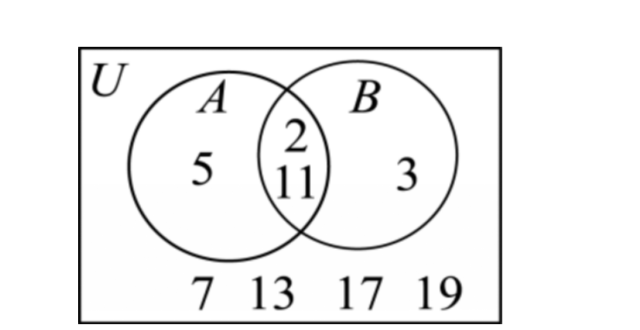
\includegraphics[width=0.24\textwidth]{figures/gao108_q6.png}
\end{center}

\solend
\fi

\item 若 $x\in A$，则 $\dfrac1x\in A$，就称 $A$ 自倒集合，集合 $M=\left\{-2,-1,0,\dfrac12,\dfrac13,1,2,3,4\right\}$ 的所有非空
子集中，自倒集合的个数为\blankline[4.4em].

\ifanswer
\solbegin
\step{由新定义，集合 $M$ 中的元素 1 和 $-1$ 倒数等于本身，2 和 $\dfrac12$，3 和 $\dfrac13$ 互为倒数,}
\step{故满足条件的自倒集合与集合 $\{-1,1,2,3\}$ 的非空子集的个数相同,}
\step{则其个数为 $2^4-1=15$.}
\solend
\fi

\item 设集合 $M=\{(x,y)\mid y=x^2+2bx+1\}$，$N=\{(x,y)\mid y=x+b\}(b\in\R)$，若
$M\cap N=\varnothing$，则实数 $b$ 的取值范围为\blankline[4.4em].

\ifanswer
\solbegin
\step{因为 $M\cap N=\varnothing$，所以
$\begin{cases}y=x^2+2bx+1\\y=x+b\end{cases}$
无解，则 $x^2+(2b-1)x+(1-b)=0$,}
\step{则 $\triangle=(2b-1)^2-4\times1\times(1-b)=4b^2-3<0$，解得 $-\dfrac{\sqrt3}2<b<\dfrac{\sqrt3}2$,}
\step{即实数 $b$ 的取值范围为 $\left(-\dfrac{\sqrt3}2,\dfrac{\sqrt3}2\right)$.}
\solend
\fi

\item 已知集合 $A=\left\{x\,\middle|\,\dfrac{x-a}{x^2-1}=1\right\}$ 有唯一元素，用列举法表示满足集合 $A$ 的条件的 $a$ 的取值集
合\blankline[4.4em].

\ifanswer
\solbegin
\step{$a=1$,$\dfrac{1}{x+1}=1$，一解；$a=-1$,$\dfrac{1}{x-1}=1$，一解；}
\step{$x-a=x^2-1$，一解时，$a=\dfrac54$,}
\step{综上，$a$ 的取值集合为 $\left\{-1,1,\dfrac54\right\}$.}
\solend
\fi

\item 已知集合 $M$ 的元素均为正整数，定义集合 $M$ 的“变项和”为：将 $M$ 中每个元素 $m$ 都乘
以 $(-1)^n$ 后再求和. 若集合 $A=\{n\mid1\leqslant n\leqslant2026,n\in\N\}$，则集合 $A$ 的所有非空子集的“变
项和”的总和为\blankline[4.4em].% $n$ 未加界定（据解析为元素序号），照录

\ifanswer
\solbegin
\step{$A=\{n\mid1\leqslant n\leqslant2026,n\in\N\}=\{1,2,\cdots,2026\}$,}
\step{1 在所有非空子集中共出现 $C_{2025}^{0}+C_{2025}^{1}+\cdots+C_{2025}^{2025}=2^{2025}$ 次,}
\step{同理 $2,3,\cdots,2026$ 都出现 $2^{2025}$ 次,}
\step{则集合 $A$ 的所有非空子集的“变项和”的总和}
\step{为 $2^{2025}\times[1\times(-1)^1+2\times(-1)^2+\cdots+2026\times(-1)^{2026}]$}
\step{$=2^{2025}\times(-1+2-3+4-\cdots-2025+2026)=1013\times2^{2025}$.}
\solend
\fi

\item 已知 $0<k<2$，定义 $[x]$ 为不超过 $x$ 的最大整数，区间 $[a,b]$（或 $(a,b)$，$[a,b)$，
$(a,b]$）的长度记为 $b-a$. 若关于 $x$ 的不等式 $k[x]>\lvert2[x]-6\rvert$ 的解集对应区间的长度为 $2$，
则 $k$ 的取值范围是\blankline[4.4em].

\ifanswer
\solbegin
\stepm{法一：}{由题意得 $\lvert2[x]-6\rvert=
\begin{cases}2[x]-6,x\geqslant3\\-2[x]+6,x<3\end{cases}$.}
\step{①当 $x\geqslant3$ 时，不等式 $k[x]>\lvert2[x]-6\rvert$ 可化为 $k[x]>2[x]-6$,}
\step{即 $(2-k)[x]<6$,}
\step{当 $0<k<2$ 时，解不等式 $(2-k)[x]<6$ 得 $[x]<\dfrac6{2-k}$.}
\step{②当 $x<3$ 时，不等式 $k[x]>\lvert2[x]-6\rvert$ 可化为 $k[x]>-2[x]+6$,}
\step{即 $(k+2)[x]>6$.}
\step{当 $0<k<2$ 时，解不等式 $(k+2)[x]>6$ 得 $[x]>\dfrac6{k+2}$.}
\step{综上所述，不等式 $k[x]>\lvert2[x]-6\rvert$ 的解集需满足 $\dfrac6{k+2}<[x]<\dfrac6{2-k}$,}
\step{由题意得在区间 $\left[\dfrac6{k+2},\dfrac6{2-k}\right]$ 内有两个整数,}
\step{由于 $\dfrac6{k+2}\in\left(\dfrac32,3\right)$，所以 $\dfrac6{2-k}\leqslant5$，得 $k\leqslant\dfrac45$.}
\step{因此 $k\in\left(0,\dfrac45\right]$，得 $\dfrac6{k+2}\in\left[\dfrac75,3\right)$，$\dfrac6{2-k}\in(3,5]$,}
\step{区间 $\left[\dfrac6{k+2},\dfrac6{2-k}\right]$ 内的两个整数是 3、4，所以 $4<\dfrac6{2-k}\leqslant5$，解得 $\dfrac12<k\leqslant\dfrac45$,}
\step{即 $k\in\left(\dfrac12,\dfrac45\right]$.}
\stepm{法二：}{令 $f(x)=kx$，$g(x)=\lvert2x-6\rvert$，画出 $g(x)$、$f(x)$ 的图象,}
\step{由于不等式 $k[x]>\lvert2[x]-6\rvert$ 的解集对应区间的长度为 2,}
\step{因此解集只可能为 $[3,5)$ 或 $[2,4)$.}
\step{当解集为 $[3,5)$ 时，如图（2），数形结合易得
$\begin{cases}f(2)\leqslant g(2)\\f(4)>g(4)\\f(5)\leqslant g(5)\end{cases}$,}
\step{即
$\begin{cases}2k\leqslant\lvert2\times2-6\rvert\\4k>\lvert2\times4-6\rvert\\5k\leqslant\lvert2\times5-6\rvert\end{cases}$，
解得
$\begin{cases}k\leqslant1\\k>\dfrac12\\k\leqslant\dfrac45\end{cases}$，
所以 $\dfrac12<k\leqslant\dfrac45$，满足 $0<k<2$,}
\step{当解集为 $[2,4)$ 时，如图（1），数形结合易得
$\begin{cases}f(2)>g(2)\\f(4)\leqslant g(4)\end{cases}$,}
\step{即
$\begin{cases}2k>\lvert2\times2-6\rvert\\4k\leqslant\lvert2\times4-6\rvert\end{cases}$，
无解.}

\begin{center}
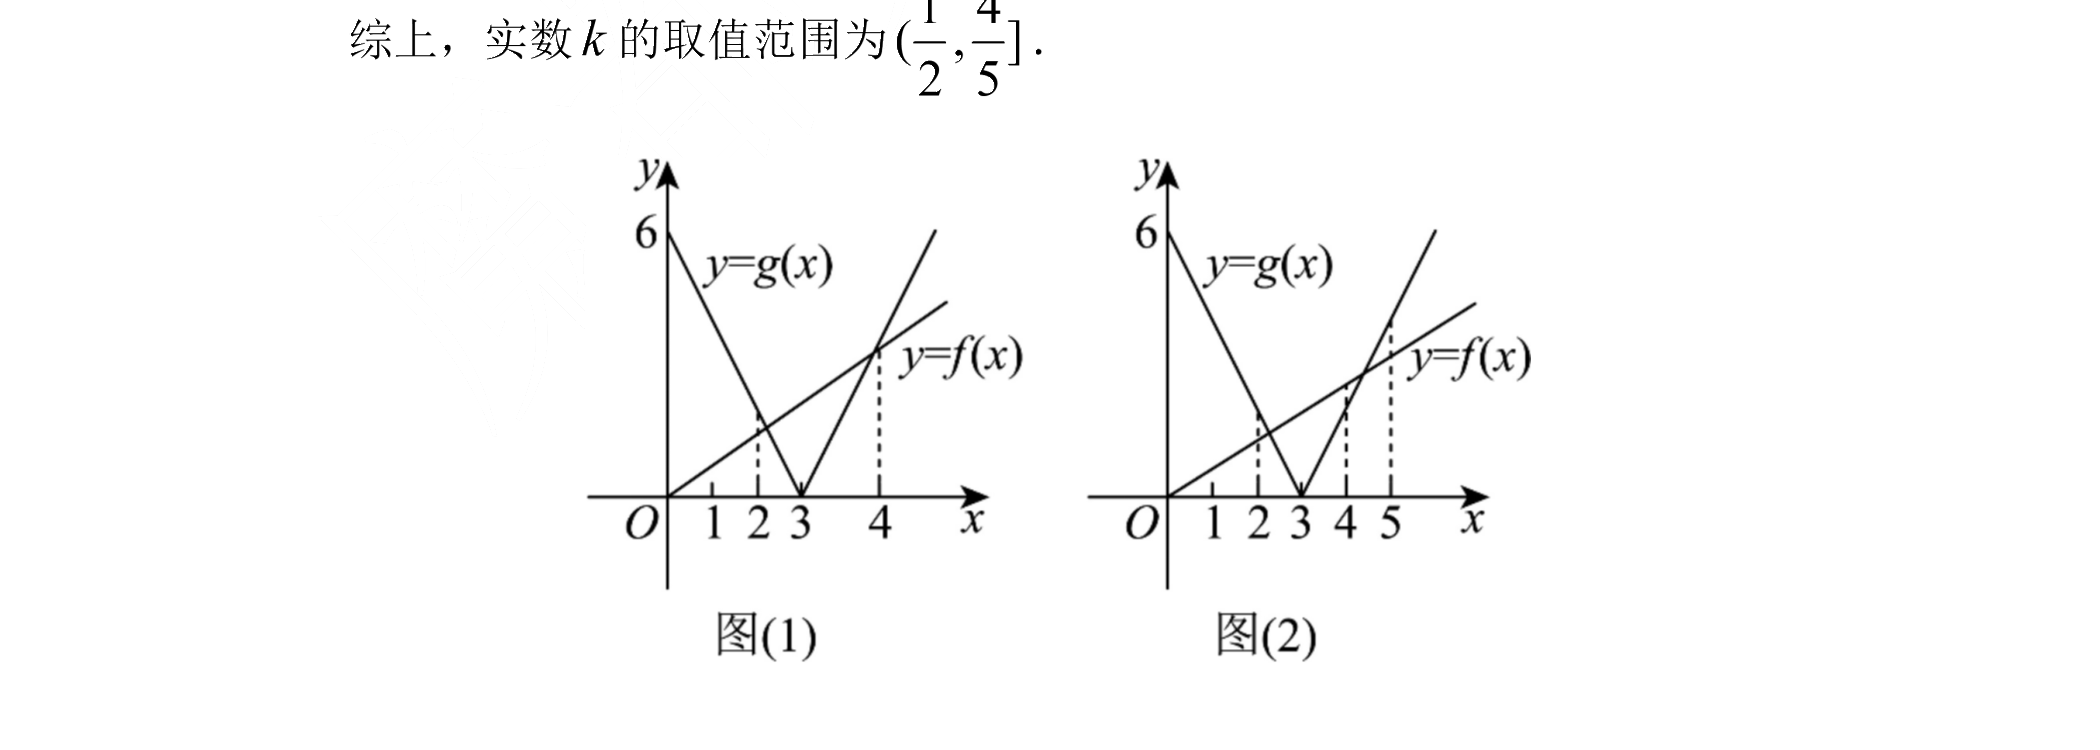
\includegraphics[width=0.72\textwidth]{figures/gao108_q11.png}
\end{center}

\step{综上，实数 $k$ 的取值范围为 $\left(\dfrac12,\dfrac45\right]$.}
\solend
\fi

\item 已知集合 $A=[1,a]\cup[a^3,a^4]$，集合 $B=\{x\mid x=x_1-x_2$，其中 $x_1$,$x_2\in A\}$. 若集合 $B$ 表
示的区间为一个闭区间，则实数 $a$ 的取值范围为\blankline[4.4em].

\ifanswer
\solbegin
\step{由题意得 $a^3>a>1$，则 $x_1-x_2$ 的最小值为 $1-a^4$，最大值为 $a^4-1$,}
\step{所以 $B=[1-a^4,a^4-1]$,}
\step{又因为 $a^4-a^3-(a-1)=a^3(a-1)-(a-1)=(a^3-1)(a-1)>0$,}
\step{所以 $a^4-a^3>a-1$，又集合 $B$ 表示的区间为一个闭区间,}
\step{则 $a^3-a\leqslant a^4-a^3$，化简得 $a^2-a-1\geqslant0$，又 $a>1$，解得 $a\geqslant\dfrac{1+\sqrt5}2$.}
\solend
\fi

\end{enumerate}

\bigsec{二、选择题}

\begin{enumerate}
\setcounter{enumi}{12}

\item 若 $a,b,c\in\R$，则下列不等式恒成立的是\mbox{（\quad）}% 原卷把答案“C”印在题干括号内、无【解析】

\keepwithprev
A. $\dfrac1a<\dfrac1b$\qquad B. $a^2<b^2$\qquad C. $\dfrac{a}{c^2+1}>\dfrac{b}{c^2+1}$\qquad D. $a\lvert c\rvert>b\lvert c\rvert$

\ifanswer
\ans{$C$}
\fi

\item 以下几个关系中正确的是\mbox{（\quad）}

\keepwithprev
A. $0\in\varnothing$\qquad\qquad\qquad B. $\varnothing\in\{x\mid x^2+1=0\}$

C. $\varnothing\subset\{0\}$\qquad\qquad\qquad D. $(A\cap B)\subset(A\cup B)$

\ifanswer
\solbegin
\step{$A$ 选项，$\varnothing$ 不包含任何元素，所以 $0\in\varnothing$ 错误，$A$ 错,}
\step{$B$ 选项，集合与集合之间关系不可以用 $\in$，$B$ 错,}
\step{$C$ 选项，空集是非空集合的真子集，所以 $\varnothing\subset\{0\}$ 正确，$C$ 对,}
\step{$D$ 选项，当 $A=B$ 时，$(A\cap B)=(A\cup B)$，$D$ 错,}
\step{故选 $C$.}
\solend
\fi

\item 设全集为 $U$，图中阴影部分所表示的集合是\mbox{（\quad）}% 原卷把答案“A”印在题干括号内、无【解析】

\keepwithprev
A. $B\cap\overline{A\cup C}$\qquad\qquad B. $(A\cup B)\cap(B\cup C)$

C. $(A\cup C)\cap\overline B$\qquad\qquad D. $(\overline A\cup\overline C)\cap B$

\ifanswer
\ans{$A$}
\fi

\item 对于 $k=0,1,2,\cdots$，定义集合 $A_k=\{20+k,26+2k\}$，并记 $S_k=A_0\cup A_1\cup\cdots\cup A_k$，则
使得集合 $S_n$ 中完全平方数的个数为奇数的最小正整数 $n$ 为\mbox{（\quad）}

\keepwithprev
A. $18$\qquad\qquad B. $19$\qquad\qquad C. $20$\qquad\qquad D. $21$

\ifanswer
\solbegin
\step{当 $k=0$ 时，$A_0=\{20,26\}$，对于 $k=0,1,2,\cdots$,}
\step{集合 $A_k$ 中最小的元素 $20>4^2$，若 $S_n$ 中完全平方数的个数为奇数，则 $n>4$,}
\step{（1）$20+k=5^2$ 时，$k=5$，$A_5=\{25,36\}$，此时 $S_5$ 中完全平方数为 $5^2$、$6^2$,}
\step{个数为 2;}
\step{$20+k=6^2$ 时，$k=16$，$A_{16}=\{36,58\}$，此时 $S_{16}$ 中完全平方数为 $5^2$、$6^2$,}
\step{个数为 2;}
\step{$20+k=7^2$ 时，$k=29$，$A_{29}=\{49,84\}$,}
\step{此时 $S_{29}$ 中完全平方数为 $5^2$、$6^2$、$7^2$、$8^2$，个数为 4;}
\step{$20+k=8^2$ 时，$k=44$，$A_{44}=\{64,114\}$,}
\step{此时 $S_{44}$ 中完全平方数为 $5^2$、$6^2$、$7^2$、$8^2$、$10^2$，个数为 5;}
\step{（2）因为 $k=0,1,2,\cdots,26+2k$ 一定为偶数,}
\step{所以 $26+2k=6^2$ 时，$k=5$，由上述分析得 $S_5$ 中完全平方数个数为 2;}
\step{$26+2k=8^2$ 时，$k=19$，$A_{19}=\{39,64\}$,}
\step{此时 $S_{19}$ 中完全平方数为 $5^2$、$6^2$、$8^2$，个数为 3.}
\step{综上，使集合 $S_n$ 中完全平方数的个数为奇数的最小正整数 $n=19$. 故选 $B$.}
\solend
\fi

\end{enumerate}

\bigsec{三、解答题}

\begin{enumerate}
\setcounter{enumi}{16}

\item 设全集 $U=\R$，集合 $A=\left\{x\,\middle|\,\dfrac{x-2}{x+2}\leqslant0\right\}$，$B=\{x\mid a\leqslant x<2a+1,a\in\R\}$，
$C=\{x\mid\lvert2x-1\rvert<5\}$.

（1）求集合 $A$、$\overline A\cup C$；

（2）若 $B\subseteq A$，求实数 $a$ 的取值范围.

\ifanswer
\solbegin
\ansspace*
\step{（1）不等式 $\dfrac{x-2}{x+2}\leqslant0$，等价于
$\begin{cases}(x-2)(x+2)\leqslant0\\x+2\neq0\end{cases}$，
解得 $\{x\mid-2<x\leqslant2\}$,}
\step{所以 $A=\{x\mid-2<x\leqslant2\}$，则 $\overline A=\{x\mid x\leqslant-2$ 或 $x>2\}$,}
\step{因为 $C=\{x\mid\lvert2x-1\rvert<5\}=\{x\mid-2<x<3\}$，所以 $\overline A\cup C=\R$；}
\step{（2）因为 $B\subseteq A$,}
\step{若 $B=\varnothing$，则 $a\geqslant2a+1$，解得 $a\leqslant-1$,}
\step{若 $B\neq\varnothing$，则
$\begin{cases}a<2a+1\\a>-2\\2a+1\leqslant2\end{cases}$，
解得 $-1<a\leqslant\dfrac12$,}
\step{综上所述，实数 $a$ 的取值范围为 $\left\{a\,\middle|\,a\leqslant\dfrac12\right\}$.}
\solend
\fi

\item 设 $a$、$b$、$c$、$d$ 是四个正数.

（1）已知 $a>b$，比较 $\dfrac{2a+b}{a+2b}$ 与 $\dfrac ab$ 的值的大小；

（2）若 $(1+a)(1+b)(1+c)(1+d)<16$，求证：$a$、$b$、$c$、$d$ 中至少有一个小于 1.

\ifanswer
\solbegin
\step{（1）$\dfrac{2a+b}{a+2b}-\dfrac ab=\dfrac{b^2-a^2}{b(a+2b)}<0$，所以 $\dfrac{2a+b}{a+2b}<\dfrac ab$.}
\step{（2）假设 $a$、$b$、$c$、$d$ 都不小于 1，即 $a$、$b$、$c$、$d$ 均大于等于 1,}
\step{即 $a\geqslant1$，$b\geqslant1$，$c\geqslant1$，$d\geqslant1$,}
\step{由均值不等式得 $1+a\geqslant2\sqrt a$,$1+b\geqslant2\sqrt b$,$1+c\geqslant2\sqrt c$,$1+d\geqslant2\sqrt d$,}
\step{故 $(1+a)(1+b)(1+c)(1+d)\geqslant16\sqrt{abcd}\geqslant16$,}
\step{当且仅当 $a=b=c=d=1$ 时取等号,}
\step{这与 $(1+a)(1+b)(1+c)(1+d)<16$ 矛盾，故假设不成立，原命题成立.}
\solend
\fi

\item 已知 $m\in\R$，一个二次项系数为 1 的一元二次方程的两个不等实根分别为 $x_1$ 和 $x_2$，且
满足
$\begin{cases}x_1^2+x_2^2=2m^2-4\\x_1+x_2=m\end{cases}$.

（1）直接写出该一元二次方程；

（2）若 $(3x_1-x_2)(3x_2-x_1)\geqslant-1$，求 $m$ 的取值范围；

（3）若方程的两根 $x_1$ 和 $x_2$ 都大于 $-1$，求 $m$ 的取值范围.

\ifanswer
\solbegin
\step{（1）设这个一元二次方程为 $x^2+bx+c=0$,}
\step{由
$\begin{cases}x_1^2+x_2^2=2m^2-4\\x_1+x_2=m\end{cases}$,}
\step{得 $(x_1+x_2)^2=x_1^2+x_2^2+2x_1x_2=2m^2-4+2x_1x_2=m^2$，即 $x_1x_2=\dfrac{4-m^2}2$,}
\step{由韦达定理得 $x_1+x_2=-b=m$，即 $x_1x_2=c=\dfrac{4-m^2}2$,}
\step{所以一元二次方程为 $x^2-mx+\dfrac{4-m^2}2=0$.}
\step{（2）$(3x_1-x_2)(3x_2-x_1)=9x_1x_2-3x_1^2-3x_2^2+x_1x_2=10x_1x_2-3(x_1^2+x_2^2)\geqslant-1$,}
\step{结合已知及（1）得 $x_1^2+x_2^2=2m^2-4$,$x_1x_2=\dfrac{4-m^2}2$,}
\step{代入得 $10\times\dfrac{4-m^2}2-3(2m^2-4)=-11m^2+32\geqslant-1\Rightarrow m^2\leqslant3$}
\step{$\Rightarrow-\sqrt3\leqslant m\leqslant\sqrt3$,}
\step{又 $\Delta=m^2-4\times\dfrac{4-m^2}2=3m^2-8>0\Rightarrow m<-\dfrac{2\sqrt6}3$ 或 $m>\dfrac{2\sqrt6}3$,}
\step{所以 $m\in\left[-\sqrt3,-\dfrac{2\sqrt6}3\right)\cup\left(\dfrac{2\sqrt6}3,\sqrt3\right]$.}
\step{（3）若方程的两根 $x_1$ 和 $x_2$ 都大于 $-1$，则
$\begin{cases}\Delta>0\\x_1+x_2>-2\\(x_1+1)(x_2+1)>0\end{cases}$,}
\step{所以
$\begin{cases}\Delta=3m^2-8>0\\m>-2\\[2pt]\dfrac{4-m^2}2+m+1>0\end{cases}$，
解得 $m\in\left(1-\sqrt7,-\dfrac{2\sqrt6}3\right)\cup\left(\dfrac{2\sqrt6}3,1+\sqrt7\right)$.}
\solend
\fi

\item 已知不等式 $2\leqslant ax^2+bx+c\leqslant3$ 的解集为 $\{x\mid2\leqslant x\leqslant3\}$.

（1）若 $a>0$，求 $6b+5c$ 的值；

（2）若 $a>0$，且不等式 $ax^2+(b-3)x-c\leqslant0$ 有且仅有 9 个整数解，求 $a$ 的取值范围；

（3）若 $a<0$，对任意的 $x<0$，不等式 $(ax-4)(x^2+b+c+1)\geqslant0$ 恒成立，求 $a^2-b+c$
的取值集合.

\ifanswer
\solbegin
\ansspace*
\step{（1）$a>0$,}
\step{结合二次函数图象得不等式 $ax^2+bx+c\leqslant3$ 的解集为 $\{x\mid2\leqslant x\leqslant3\}$,}
\step{且不等式 $ax^2+bx+c\geqslant2$ 的解集为 $R$,}
\step{所以方程 $ax^2+bx+c-3=0$ 的两根分别为 2 和 3,}
\step{则
$\begin{cases}2+3=-\dfrac ba\\[2pt]2\times3=\dfrac{c-3}a\end{cases}$，
得 $b=-5a$，$c=6a+3$,}
\step{所以 $6b+5c=6\times(-5a)+5(6a+3)=15$.}
\step{（2）若 $a>0$，且不等式 $ax^2+(b-3)x-c\leqslant0$ 有且仅有 9 个整数解,}
\step{由（1）得 $b=-5a$，$c=6a+3$,}
\step{不等式 $ax^2+bx+c\geqslant2$ 可化为 $ax^2-5ax+6a+1\geqslant0$.}
\step{由（1）得不等式 $ax^2+bx+c\geqslant2$ 的解集为 $R$,}
\step{所以 $ax^2-5ax+6a+1\geqslant0$ 恒成立,}
\step{所以
$\begin{cases}a>0\\\Delta=25a^2-4a(6a+1)\leqslant0\end{cases}$，
即
$\begin{cases}a>0\\a^2-4a=a(a-4)\leqslant0\end{cases}$，}
\step{解得 $0<a\leqslant4$.}
\step{不等式 $ax^2+(b-3)x-c\leqslant0$ 等价于 $ax^2-(5a+3)x-(6a+3)\leqslant0$,}
\step{所以 $[ax-(6a+3)](x+1)\leqslant0$，得 $-1\leqslant x\leqslant6+\dfrac3a$,}
\step{所以 $7\leqslant6+\dfrac3a<8$，解得 $\dfrac32<a\leqslant3$.}
\step{综上，$a$ 的取值范围为 $\left(\dfrac32,3\right]$.}
\step{（3）因为 $a<0$,}
\step{同（1）分析，不等式 $ax^2+bx+c\geqslant2$ 的解集为 $\{x\mid2\leqslant x\leqslant3\}$,}
\step{$ax^2+bx+c\leqslant3$ 的解集为 $R$,}
\step{所以方程 $ax^2+bx+c-2=0$ 的两根分别为 2 和 3,}
\step{则
$\begin{cases}2+3=-\dfrac ba\\[2pt]2\times3=\dfrac{c-2}a\end{cases}$，
得 $b=-5a$，$c=6a+2$.}
\step{所以不等式 $ax^2+bx+c=ax^2-5ax+6a+2\leqslant3$ 的解集为 $R$,}
\step{则 $ax^2-5ax+6a-1\leqslant0$ 恒成立,}
\step{所以
$\begin{cases}a<0\\\Delta=25a^2-4a(6a-1)\leqslant0\end{cases}$，
即
$\begin{cases}a<0\\a^2+4a=a(a+4)\leqslant0\end{cases}$，}
\step{解得 $-4\leqslant a<0$.}
\step{所以对任意的 $x<0$，不等式 $(ax-4)(x^2+b+c+1)\geqslant0$ 恒成立}
\step{转化为对任意的 $x<0$，不等式 $(ax-4)(x^2+a+3)\geqslant0$ 恒成立.}
\step{方程 $(ax-4)(x^2+a+3)=0$ 的两个根为 $x=\dfrac4a<0$,}
\step{$x=\pm\sqrt{-a-3}$（$a<-3$ 时成立）,}
\step{因而仅当 $ax-4=0$ 与 $x^2+a+3=0$ 的负根重合时满足条件,}
\step{解得唯一解为 $a=-4$，所以 $a^2-b+c=a^2+11a+2=-26$,}
\step{所以 $a^2-b+c$ 的取值集合为 $\{-26\}$.}
\solend
\fi

\item 已知集合 $A=\{1,2,3,4,5,6,7,8\}$，$M=\{(x,y)\mid x\in A,y\in A\}$，从 $M$ 中选取 $n$ 个不同的
元素组成一个序列：$(x_1,y_1)$,$(x_2,y_2),\cdots,(x_n,y_n)$，其中 $(x_i,y_i)$ 称为该序列的第 $i$ 项
（$i=1,2,\cdots,n$），若该序列的相邻项 $(x_i,y_i)$,$(x_{i+1},y_{i+1})$ 满足：
\[\begin{cases}\lvert x_{i+1}-x_i\rvert=3\\\lvert y_{i+1}-y_i\rvert=4\end{cases}
\quad\text{或}\quad
\begin{cases}\lvert x_{i+1}-x_i\rvert=4\\\lvert y_{i+1}-y_i\rvert=3\end{cases}\]
（$i=1,2,\cdots,n-1$），则称该序列为“$\Delta-$序列”.

（1）若一个 $\Delta-$序列的第一项为 $(4,4)$，请直接写出它所有可能的第二项；

（2）定义集合 $A=\{1,2,3,4,5,6,7,8\}$ 的两个子集：外侧集 $S=\{1,2,7,8\}$，内侧集
$T=\{3,4,5,6\}$. 证明：若 $\Delta-$序列中某一项的坐标在区域 $S\times S$ 内（即横、纵坐标均属于
$S$），则它的下一项坐标必定在区域 $T\times T$ 内；

（3）证明：不存在一个恰好有 5 项的 $\Delta-$序列，使其第一项为 $(1,8)$，且第五项为
$(8,1)$.

\ifanswer
\solbegin
\ansspace*
\step{（1）由题意，第一项为 $(x_1,y_1)=(4,4)$,}
\step{对于第二项 $(x_2,y_2)$，其坐标必须在 1~8 之间.}
\step{若 $\lvert x_2-4\rvert=3$,$\lvert y_2-4\rvert=4$，则 $x_2\in\{1,7\}$,}
\step{且 $y_2\in\{8\}$（因为 $4-4=0$ 不在集合 $A$ 中）. 此时可能的点为 $(1,8)$,$(7,8)$.}
\step{若 $\lvert x_2-4\rvert=4$,$\lvert y_2-4\rvert=3$，则 $x_2\in\{8\}$，且 $y_2\in\{1,7\}$.}
\step{此时可能的点为 $(8,1)$,$(8,7)$.}
\step{所以它所有可能的第二项为 $(1,8)$,$(7,8)$,$(8,1)$,$(8,7)$.}
\step{（2）已知某一项 $(x_t,y_t)\in S\times S$，即 $x_t\in\{1,2,7,8\}$ 且 $y_t\in\{1,2,7,8\}$.}
\step{由规则得下一步坐标的变化量为 3 和 4，设 $a\in S$ 变化 3 或 4 后的结果 $a'$:}
\step{当 $a=1$ 时，$1+3=4\in T$,$1+4=5\in T$；}
\step{当 $a=2$ 时，$2+3=5\in T$,$2+4=6\in T$；}
\step{当 $a=7$ 时，$7-3=4\in T$,$7-4=3\in T$；}
\step{当 $a=8$ 时，$8-3=5\in T$,$8-4=4\in T$.}
\step{（注：由于超出 1~8 范围的越界坐标不符合.）}
\step{由此可见，无论 $a$ 是 $S$ 中的哪一个数，加上或减去 3 或 4 之后,}
\step{得到的新坐标必属于集合 $T$.}
\step{因为 $\Delta-$序列每走一步，横坐标和纵坐标必定同时发生 3 和 4 的变化,}
\step{所以新的横坐标 $x_{i+1}$ 必属于 $T$，新的纵坐标 $y_{i+1}$ 也必属于 $T$,}
\step{即下一项 $(x_{i+1},y_{i+1})$ 必定在区域 $T\times T$ 内. ………10 分原命题得证.% 得分行混入证明，照录
}
\step{（3）假设存在这样一个包含 5 项的 $\Delta-$序列:}
\step{$(x_1,y_1)$,$(x_2,y_2)$,$(x_3,y_3)$,$(x_4,y_4)$,$(x_5,y_5)$.}
\step{已知第一项为 $(1,8)$，第五项为 $(8,1)$. 第 2 项必须是第 1 项 $(1,8)$ 的相邻点.}
\step{我们来找 $(1,8)$ 的相邻点：第 2 项只能是 $(4,4)$ 或 $(5,5)$,}
\step{第 4 项必须是第 5 项 $(8,1)$ 的相邻点（因为跳跃是双向可逆的）.}
\step{同理可算得，$(8,1)$ 的相邻点也只有两个：$(4,4)$ 和 $(5,5)$,}
\step{题目题干中明确规定，$\Delta-$序列由 $n$ 个不同的有序数对构成.% “题目题干”措辞重复，照录
}
\step{所以，第 2 项和第 4 项不能是同一个点. 这就意味着:}
\step{如果第 2 项是 $(4,4)$，第 4 项就必须是 $(5,5)$；反之亦然.}
\step{则第 3 项必须是 $(4,4)$ 和 $(5,5)$ 的公共相邻点.}
\step{$(4,4)$ 的相邻点集合为：$\{(1,8),(7,8),(8,1),(8,7)\}$,}
\step{$(5,5)$ 的相邻点集合为：$\{(2,1),(8,1),(1,2),(1,8)\}$,}
\step{所以，第 3 项只能填 $(1,8)$ 或者 $(8,1)$.}
\step{这与“序列由不同的有序数对构成”这一条件产生矛盾！}
\step{所以，不存在一个恰好有 5 项的 $\Delta-$序列,}
\step{使其第一项为 $(1,8)$，且第五项为 $(8,1)$.}
\solend
\fi

\end{enumerate}

\end{document}
"
% 紧凑版：xelatex "\def\iscompact{1}% 高一108_五校联考_10月月考.tex
%   —— 高一上数学“2026-2027 年五校联考高一上 10 月月考”（试卷版/答案版）
% 试卷版：xelatex 高一108_五校联考_10月月考.tex
% 答案版：xelatex "\def\isanswer{1}% 高一108_五校联考_10月月考.tex
%   —— 高一上数学“2026-2027 年五校联考高一上 10 月月考”（试卷版/答案版）
% 试卷版：xelatex 高一108_五校联考_10月月考.tex
% 答案版：xelatex "\def\isanswer{1}% 高一108_五校联考_10月月考.tex
%   —— 高一上数学“2026-2027 年五校联考高一上 10 月月考”（试卷版/答案版）
% 试卷版：xelatex 高一108_五校联考_10月月考.tex
% 答案版：xelatex "\def\isanswer{1}\input{高一108_五校联考_10月月考.tex}"
% 紧凑版：xelatex "\def\iscompact{1}\input{高一108_五校联考_10月月考.tex}"
%
% 原始材料：微信公众号“魔都数学加油站”文章，作者破晓，2026-11-03 17:19 发布；
% 连载“27学年高一108”，原文标题“27学年高一108——2026-2027年上海市五校联考高一上10月月考”；
% 原文链接：https://mp.weixin.qq.com/s/3nkP789Qar93NGMZXFFCSw。
% 正文为 14 张 PNG 页（第 2、3、6—13 页 4762×6735，第 1、4、5、14 页 2560×3620），
% 题目下印有【解析】，为讲评版。
% 题目、解析均据原图转录；卷面水印及公众号页脚未录入。
% 第 6 题解析的文氏图与第 11 题法二解析的两幅图象（图(1)、图(2)）裁自原图、去粉色水印
% 转灰度（gao108_q6.png、gao108_q11.png），第 6 题图属解析（仅答案版）、
% 第 11 题图属解析（仅答案版）。
%
% 卷首标题：原卷印作“2026-2027 年五校联考高一上 10 月月考”，标题下另印一行参与学校
% 名单“闵行中学、嘉定一中、松江一中、金山中学、嘉一实高”（全稿第 5 份原卷自印副标题，
% 按 14／24／49／50 成例照录，并登记进计数核对.py 的 SELFSUB）。
%
% 与原卷的排版差异：
%   ① 原文从第 3 题起，填空题编号为 3—12、选择题为 13—16、解答题为 17—21，本稿保留原题号；
%   ② 原卷每题下直接印【解析】，本稿按全稿惯例将解析置于答案版；第 4 题只印【答案】，
%      第 13、15 两题把答案印在题干括号内且无【解析】，均另提 \ans{}；
%   ③ 原卷副标题照录（见上）；
%   ④ 原卷填空横线按全稿惯例排为 \blankline[4.4em]；解答题按惯例加 \ansspace；选择题括号排
%      \mbox{（\quad）}、选项段前按惯例加 \keepwithprev；
%   ⑤ 原卷数集排斜体 $R$／$N$，按全稿惯例改 \R、\N。
%
% 原卷红色强调照录为黑体：第 11 题解析的“法一：”“法二：”原卷排红色，按 53 成例排
% \stepm{法一：}／\stepm{法二：}（加粗着色）。
%
% 原卷存疑：第 10 题题干“变项和”定义中“将 $M$ 中每个元素 $m$ 都乘以 $(-1)^n$ 后再求和”
% 的 $n$ 未加界定（据解析应为该元素在 $\{1,2,\cdots,2026\}$ 中的序号），照录。
% 第 21 题 (2) 解析末行“即下一项 $(x_{i+1},y_{i+1})$ 必定在区域 $T\times T$ 内. ………10 分
% 原命题得证.”，原卷把得分点行混入证明（“原命题”按上下文为“原命题的逆否”），照录。
% 第 21 题 (3) 解析“题目题干中明确规定”，“题目题干”措辞重复，照录。
%
% 行数核对：逐题数 \step/\stepm 条数，合计 164 条（Q3：3；Q4：0；Q5：2；Q6：1；Q7：3；
% Q8：3；Q9：3；Q10：6；Q11：21；Q12：5；Q13：0；Q14：5；Q15：0；Q16：15；Q17：7；
% Q18：7；Q19：13；Q20：34；Q21：36），与原卷印刷行逐题相等。第 4 题只印【答案】、
% 第 13、15 题括号内印答案，均提 \ans{}，不计入 \step 账。
%
\documentclass[a4paper,11pt]{article}
\usepackage{common}

\begin{document}

\examtitlest[3]{2026--2027 年五校联考高一上 10 月月考}{闵行中学、嘉定一中、松江一中、金山中学、嘉一实高}

\bigsec{一、填空题}

\begin{enumerate}
\setcounter{enumi}{2}

\item 已知等式 $2x^2+3x+5=2ax^2+a(3x+1)+c$ 恒成立，则实数 $a+c$ 的值为\blankline[4.4em].

\ifanswer
\solbegin
\step{因为 $2x^2+3x+5=2ax^2+a(3x+1)+c$ 恒成立,}
\step{即 $2x^2+3x+5=2ax^2+3ax+(a+c)$ 恒成立，所以
$\begin{cases}2=2a\\3=3a\\5=a+c\end{cases}$,}
\step{所以 $a+c=5$.}
\solend
\fi

\item 不等式 $\dfrac1x<\dfrac12$ 的解集是\blankline[4.4em].

\ifanswer
\ans{$(-\infty,0)\cup(2,+\infty)$}
\fi

\item 已知 $a$、$b$ 都是实数，则“$a^2=b^2$”是“$a^2+b^2=2ab$”的\blankline[4.4em]条件.

\ifanswer
\solbegin
\step{$a^2=b^2$ 等价于 $a=\pm b$；$a^2+b^2=2ab$ 等价于 $(a-b)^2=0$ 等价于 $a=b$,}
\step{故“$a^2=b^2$”是“$a^2+b^2=2ab$”的必要不充分条件.}
\solend
\fi

\item 已知全集 $U=\{x\mid x$ 为不大于 20 的素数$\}$，$A\cap\overline B=\{5\}$，$\overline A\cap B=\{3\}$，
$\overline{A\cup B}=\{7,13,17,19\}$，则 $A=$\blankline[4.4em].

\ifanswer
\solbegin
\step{如图所示，$A=\{2,5,11\}$.}

\begin{center}
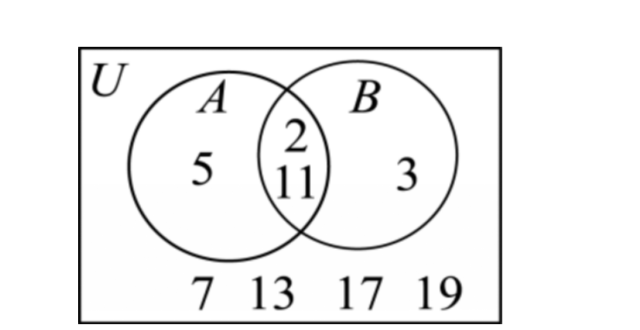
\includegraphics[width=0.24\textwidth]{figures/gao108_q6.png}
\end{center}

\solend
\fi

\item 若 $x\in A$，则 $\dfrac1x\in A$，就称 $A$ 自倒集合，集合 $M=\left\{-2,-1,0,\dfrac12,\dfrac13,1,2,3,4\right\}$ 的所有非空
子集中，自倒集合的个数为\blankline[4.4em].

\ifanswer
\solbegin
\step{由新定义，集合 $M$ 中的元素 1 和 $-1$ 倒数等于本身，2 和 $\dfrac12$，3 和 $\dfrac13$ 互为倒数,}
\step{故满足条件的自倒集合与集合 $\{-1,1,2,3\}$ 的非空子集的个数相同,}
\step{则其个数为 $2^4-1=15$.}
\solend
\fi

\item 设集合 $M=\{(x,y)\mid y=x^2+2bx+1\}$，$N=\{(x,y)\mid y=x+b\}(b\in\R)$，若
$M\cap N=\varnothing$，则实数 $b$ 的取值范围为\blankline[4.4em].

\ifanswer
\solbegin
\step{因为 $M\cap N=\varnothing$，所以
$\begin{cases}y=x^2+2bx+1\\y=x+b\end{cases}$
无解，则 $x^2+(2b-1)x+(1-b)=0$,}
\step{则 $\triangle=(2b-1)^2-4\times1\times(1-b)=4b^2-3<0$，解得 $-\dfrac{\sqrt3}2<b<\dfrac{\sqrt3}2$,}
\step{即实数 $b$ 的取值范围为 $\left(-\dfrac{\sqrt3}2,\dfrac{\sqrt3}2\right)$.}
\solend
\fi

\item 已知集合 $A=\left\{x\,\middle|\,\dfrac{x-a}{x^2-1}=1\right\}$ 有唯一元素，用列举法表示满足集合 $A$ 的条件的 $a$ 的取值集
合\blankline[4.4em].

\ifanswer
\solbegin
\step{$a=1$,$\dfrac{1}{x+1}=1$，一解；$a=-1$,$\dfrac{1}{x-1}=1$，一解；}
\step{$x-a=x^2-1$，一解时，$a=\dfrac54$,}
\step{综上，$a$ 的取值集合为 $\left\{-1,1,\dfrac54\right\}$.}
\solend
\fi

\item 已知集合 $M$ 的元素均为正整数，定义集合 $M$ 的“变项和”为：将 $M$ 中每个元素 $m$ 都乘
以 $(-1)^n$ 后再求和. 若集合 $A=\{n\mid1\leqslant n\leqslant2026,n\in\N\}$，则集合 $A$ 的所有非空子集的“变
项和”的总和为\blankline[4.4em].% $n$ 未加界定（据解析为元素序号），照录

\ifanswer
\solbegin
\step{$A=\{n\mid1\leqslant n\leqslant2026,n\in\N\}=\{1,2,\cdots,2026\}$,}
\step{1 在所有非空子集中共出现 $C_{2025}^{0}+C_{2025}^{1}+\cdots+C_{2025}^{2025}=2^{2025}$ 次,}
\step{同理 $2,3,\cdots,2026$ 都出现 $2^{2025}$ 次,}
\step{则集合 $A$ 的所有非空子集的“变项和”的总和}
\step{为 $2^{2025}\times[1\times(-1)^1+2\times(-1)^2+\cdots+2026\times(-1)^{2026}]$}
\step{$=2^{2025}\times(-1+2-3+4-\cdots-2025+2026)=1013\times2^{2025}$.}
\solend
\fi

\item 已知 $0<k<2$，定义 $[x]$ 为不超过 $x$ 的最大整数，区间 $[a,b]$（或 $(a,b)$，$[a,b)$，
$(a,b]$）的长度记为 $b-a$. 若关于 $x$ 的不等式 $k[x]>\lvert2[x]-6\rvert$ 的解集对应区间的长度为 $2$，
则 $k$ 的取值范围是\blankline[4.4em].

\ifanswer
\solbegin
\stepm{法一：}{由题意得 $\lvert2[x]-6\rvert=
\begin{cases}2[x]-6,x\geqslant3\\-2[x]+6,x<3\end{cases}$.}
\step{①当 $x\geqslant3$ 时，不等式 $k[x]>\lvert2[x]-6\rvert$ 可化为 $k[x]>2[x]-6$,}
\step{即 $(2-k)[x]<6$,}
\step{当 $0<k<2$ 时，解不等式 $(2-k)[x]<6$ 得 $[x]<\dfrac6{2-k}$.}
\step{②当 $x<3$ 时，不等式 $k[x]>\lvert2[x]-6\rvert$ 可化为 $k[x]>-2[x]+6$,}
\step{即 $(k+2)[x]>6$.}
\step{当 $0<k<2$ 时，解不等式 $(k+2)[x]>6$ 得 $[x]>\dfrac6{k+2}$.}
\step{综上所述，不等式 $k[x]>\lvert2[x]-6\rvert$ 的解集需满足 $\dfrac6{k+2}<[x]<\dfrac6{2-k}$,}
\step{由题意得在区间 $\left[\dfrac6{k+2},\dfrac6{2-k}\right]$ 内有两个整数,}
\step{由于 $\dfrac6{k+2}\in\left(\dfrac32,3\right)$，所以 $\dfrac6{2-k}\leqslant5$，得 $k\leqslant\dfrac45$.}
\step{因此 $k\in\left(0,\dfrac45\right]$，得 $\dfrac6{k+2}\in\left[\dfrac75,3\right)$，$\dfrac6{2-k}\in(3,5]$,}
\step{区间 $\left[\dfrac6{k+2},\dfrac6{2-k}\right]$ 内的两个整数是 3、4，所以 $4<\dfrac6{2-k}\leqslant5$，解得 $\dfrac12<k\leqslant\dfrac45$,}
\step{即 $k\in\left(\dfrac12,\dfrac45\right]$.}
\stepm{法二：}{令 $f(x)=kx$，$g(x)=\lvert2x-6\rvert$，画出 $g(x)$、$f(x)$ 的图象,}
\step{由于不等式 $k[x]>\lvert2[x]-6\rvert$ 的解集对应区间的长度为 2,}
\step{因此解集只可能为 $[3,5)$ 或 $[2,4)$.}
\step{当解集为 $[3,5)$ 时，如图（2），数形结合易得
$\begin{cases}f(2)\leqslant g(2)\\f(4)>g(4)\\f(5)\leqslant g(5)\end{cases}$,}
\step{即
$\begin{cases}2k\leqslant\lvert2\times2-6\rvert\\4k>\lvert2\times4-6\rvert\\5k\leqslant\lvert2\times5-6\rvert\end{cases}$，
解得
$\begin{cases}k\leqslant1\\k>\dfrac12\\k\leqslant\dfrac45\end{cases}$，
所以 $\dfrac12<k\leqslant\dfrac45$，满足 $0<k<2$,}
\step{当解集为 $[2,4)$ 时，如图（1），数形结合易得
$\begin{cases}f(2)>g(2)\\f(4)\leqslant g(4)\end{cases}$,}
\step{即
$\begin{cases}2k>\lvert2\times2-6\rvert\\4k\leqslant\lvert2\times4-6\rvert\end{cases}$，
无解.}

\begin{center}
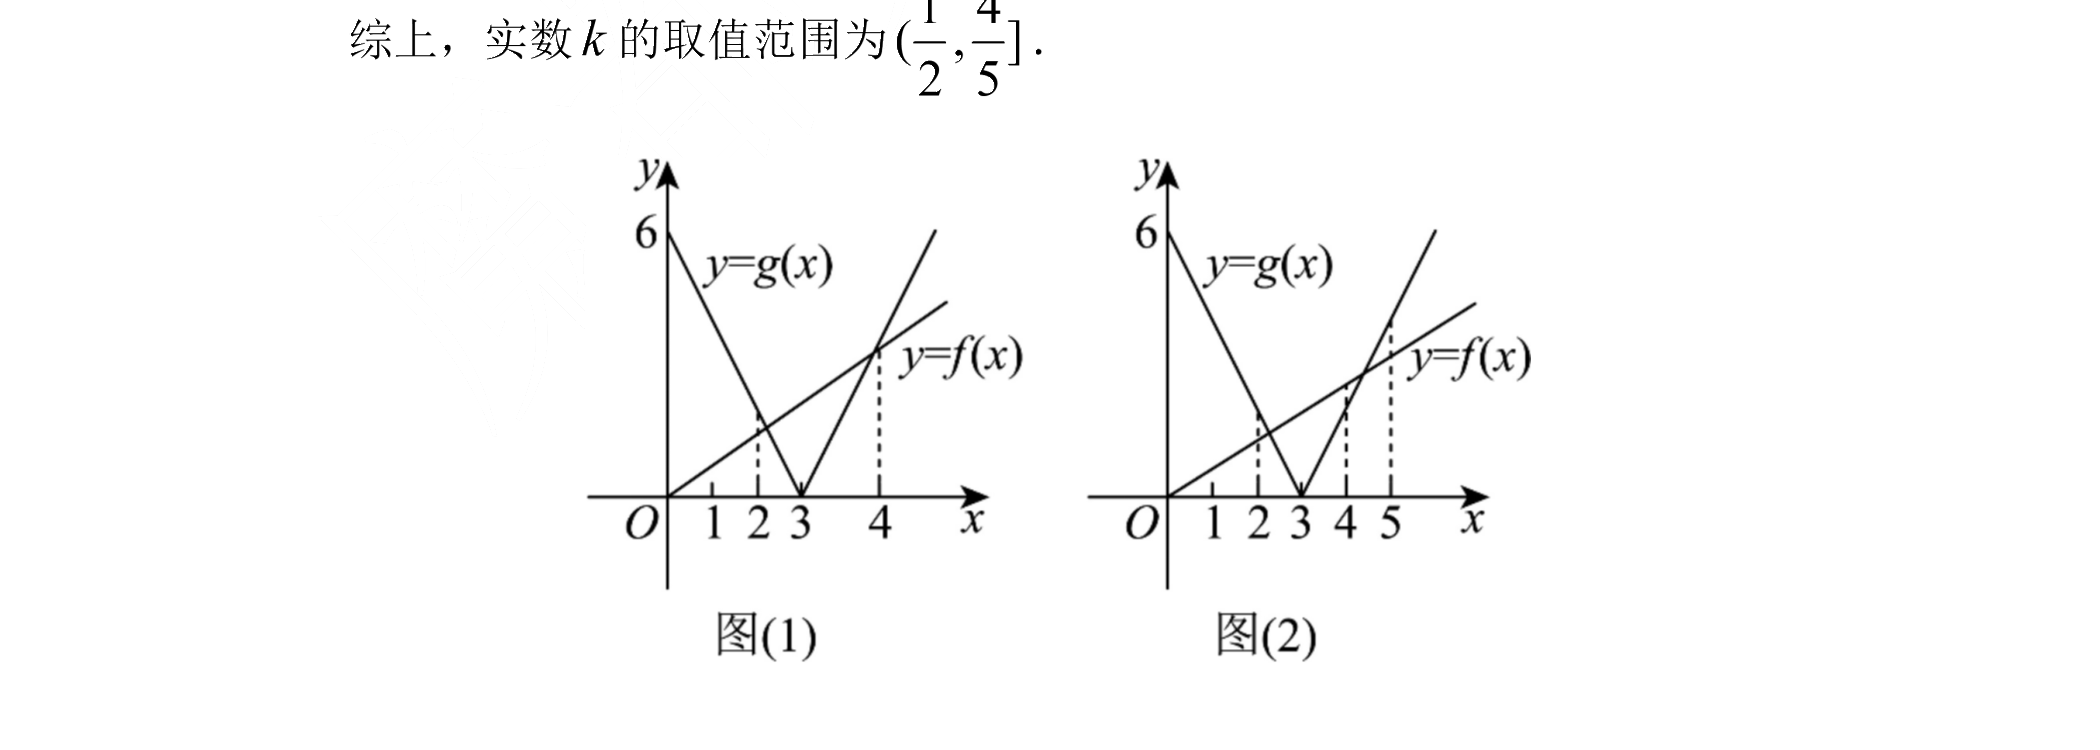
\includegraphics[width=0.72\textwidth]{figures/gao108_q11.png}
\end{center}

\step{综上，实数 $k$ 的取值范围为 $\left(\dfrac12,\dfrac45\right]$.}
\solend
\fi

\item 已知集合 $A=[1,a]\cup[a^3,a^4]$，集合 $B=\{x\mid x=x_1-x_2$，其中 $x_1$,$x_2\in A\}$. 若集合 $B$ 表
示的区间为一个闭区间，则实数 $a$ 的取值范围为\blankline[4.4em].

\ifanswer
\solbegin
\step{由题意得 $a^3>a>1$，则 $x_1-x_2$ 的最小值为 $1-a^4$，最大值为 $a^4-1$,}
\step{所以 $B=[1-a^4,a^4-1]$,}
\step{又因为 $a^4-a^3-(a-1)=a^3(a-1)-(a-1)=(a^3-1)(a-1)>0$,}
\step{所以 $a^4-a^3>a-1$，又集合 $B$ 表示的区间为一个闭区间,}
\step{则 $a^3-a\leqslant a^4-a^3$，化简得 $a^2-a-1\geqslant0$，又 $a>1$，解得 $a\geqslant\dfrac{1+\sqrt5}2$.}
\solend
\fi

\end{enumerate}

\bigsec{二、选择题}

\begin{enumerate}
\setcounter{enumi}{12}

\item 若 $a,b,c\in\R$，则下列不等式恒成立的是\mbox{（\quad）}% 原卷把答案“C”印在题干括号内、无【解析】

\keepwithprev
A. $\dfrac1a<\dfrac1b$\qquad B. $a^2<b^2$\qquad C. $\dfrac{a}{c^2+1}>\dfrac{b}{c^2+1}$\qquad D. $a\lvert c\rvert>b\lvert c\rvert$

\ifanswer
\ans{$C$}
\fi

\item 以下几个关系中正确的是\mbox{（\quad）}

\keepwithprev
A. $0\in\varnothing$\qquad\qquad\qquad B. $\varnothing\in\{x\mid x^2+1=0\}$

C. $\varnothing\subset\{0\}$\qquad\qquad\qquad D. $(A\cap B)\subset(A\cup B)$

\ifanswer
\solbegin
\step{$A$ 选项，$\varnothing$ 不包含任何元素，所以 $0\in\varnothing$ 错误，$A$ 错,}
\step{$B$ 选项，集合与集合之间关系不可以用 $\in$，$B$ 错,}
\step{$C$ 选项，空集是非空集合的真子集，所以 $\varnothing\subset\{0\}$ 正确，$C$ 对,}
\step{$D$ 选项，当 $A=B$ 时，$(A\cap B)=(A\cup B)$，$D$ 错,}
\step{故选 $C$.}
\solend
\fi

\item 设全集为 $U$，图中阴影部分所表示的集合是\mbox{（\quad）}% 原卷把答案“A”印在题干括号内、无【解析】

\keepwithprev
A. $B\cap\overline{A\cup C}$\qquad\qquad B. $(A\cup B)\cap(B\cup C)$

C. $(A\cup C)\cap\overline B$\qquad\qquad D. $(\overline A\cup\overline C)\cap B$

\ifanswer
\ans{$A$}
\fi

\item 对于 $k=0,1,2,\cdots$，定义集合 $A_k=\{20+k,26+2k\}$，并记 $S_k=A_0\cup A_1\cup\cdots\cup A_k$，则
使得集合 $S_n$ 中完全平方数的个数为奇数的最小正整数 $n$ 为\mbox{（\quad）}

\keepwithprev
A. $18$\qquad\qquad B. $19$\qquad\qquad C. $20$\qquad\qquad D. $21$

\ifanswer
\solbegin
\step{当 $k=0$ 时，$A_0=\{20,26\}$，对于 $k=0,1,2,\cdots$,}
\step{集合 $A_k$ 中最小的元素 $20>4^2$，若 $S_n$ 中完全平方数的个数为奇数，则 $n>4$,}
\step{（1）$20+k=5^2$ 时，$k=5$，$A_5=\{25,36\}$，此时 $S_5$ 中完全平方数为 $5^2$、$6^2$,}
\step{个数为 2;}
\step{$20+k=6^2$ 时，$k=16$，$A_{16}=\{36,58\}$，此时 $S_{16}$ 中完全平方数为 $5^2$、$6^2$,}
\step{个数为 2;}
\step{$20+k=7^2$ 时，$k=29$，$A_{29}=\{49,84\}$,}
\step{此时 $S_{29}$ 中完全平方数为 $5^2$、$6^2$、$7^2$、$8^2$，个数为 4;}
\step{$20+k=8^2$ 时，$k=44$，$A_{44}=\{64,114\}$,}
\step{此时 $S_{44}$ 中完全平方数为 $5^2$、$6^2$、$7^2$、$8^2$、$10^2$，个数为 5;}
\step{（2）因为 $k=0,1,2,\cdots,26+2k$ 一定为偶数,}
\step{所以 $26+2k=6^2$ 时，$k=5$，由上述分析得 $S_5$ 中完全平方数个数为 2;}
\step{$26+2k=8^2$ 时，$k=19$，$A_{19}=\{39,64\}$,}
\step{此时 $S_{19}$ 中完全平方数为 $5^2$、$6^2$、$8^2$，个数为 3.}
\step{综上，使集合 $S_n$ 中完全平方数的个数为奇数的最小正整数 $n=19$. 故选 $B$.}
\solend
\fi

\end{enumerate}

\bigsec{三、解答题}

\begin{enumerate}
\setcounter{enumi}{16}

\item 设全集 $U=\R$，集合 $A=\left\{x\,\middle|\,\dfrac{x-2}{x+2}\leqslant0\right\}$，$B=\{x\mid a\leqslant x<2a+1,a\in\R\}$，
$C=\{x\mid\lvert2x-1\rvert<5\}$.

（1）求集合 $A$、$\overline A\cup C$；

（2）若 $B\subseteq A$，求实数 $a$ 的取值范围.

\ifanswer
\solbegin
\ansspace*
\step{（1）不等式 $\dfrac{x-2}{x+2}\leqslant0$，等价于
$\begin{cases}(x-2)(x+2)\leqslant0\\x+2\neq0\end{cases}$，
解得 $\{x\mid-2<x\leqslant2\}$,}
\step{所以 $A=\{x\mid-2<x\leqslant2\}$，则 $\overline A=\{x\mid x\leqslant-2$ 或 $x>2\}$,}
\step{因为 $C=\{x\mid\lvert2x-1\rvert<5\}=\{x\mid-2<x<3\}$，所以 $\overline A\cup C=\R$；}
\step{（2）因为 $B\subseteq A$,}
\step{若 $B=\varnothing$，则 $a\geqslant2a+1$，解得 $a\leqslant-1$,}
\step{若 $B\neq\varnothing$，则
$\begin{cases}a<2a+1\\a>-2\\2a+1\leqslant2\end{cases}$，
解得 $-1<a\leqslant\dfrac12$,}
\step{综上所述，实数 $a$ 的取值范围为 $\left\{a\,\middle|\,a\leqslant\dfrac12\right\}$.}
\solend
\fi

\item 设 $a$、$b$、$c$、$d$ 是四个正数.

（1）已知 $a>b$，比较 $\dfrac{2a+b}{a+2b}$ 与 $\dfrac ab$ 的值的大小；

（2）若 $(1+a)(1+b)(1+c)(1+d)<16$，求证：$a$、$b$、$c$、$d$ 中至少有一个小于 1.

\ifanswer
\solbegin
\step{（1）$\dfrac{2a+b}{a+2b}-\dfrac ab=\dfrac{b^2-a^2}{b(a+2b)}<0$，所以 $\dfrac{2a+b}{a+2b}<\dfrac ab$.}
\step{（2）假设 $a$、$b$、$c$、$d$ 都不小于 1，即 $a$、$b$、$c$、$d$ 均大于等于 1,}
\step{即 $a\geqslant1$，$b\geqslant1$，$c\geqslant1$，$d\geqslant1$,}
\step{由均值不等式得 $1+a\geqslant2\sqrt a$,$1+b\geqslant2\sqrt b$,$1+c\geqslant2\sqrt c$,$1+d\geqslant2\sqrt d$,}
\step{故 $(1+a)(1+b)(1+c)(1+d)\geqslant16\sqrt{abcd}\geqslant16$,}
\step{当且仅当 $a=b=c=d=1$ 时取等号,}
\step{这与 $(1+a)(1+b)(1+c)(1+d)<16$ 矛盾，故假设不成立，原命题成立.}
\solend
\fi

\item 已知 $m\in\R$，一个二次项系数为 1 的一元二次方程的两个不等实根分别为 $x_1$ 和 $x_2$，且
满足
$\begin{cases}x_1^2+x_2^2=2m^2-4\\x_1+x_2=m\end{cases}$.

（1）直接写出该一元二次方程；

（2）若 $(3x_1-x_2)(3x_2-x_1)\geqslant-1$，求 $m$ 的取值范围；

（3）若方程的两根 $x_1$ 和 $x_2$ 都大于 $-1$，求 $m$ 的取值范围.

\ifanswer
\solbegin
\step{（1）设这个一元二次方程为 $x^2+bx+c=0$,}
\step{由
$\begin{cases}x_1^2+x_2^2=2m^2-4\\x_1+x_2=m\end{cases}$,}
\step{得 $(x_1+x_2)^2=x_1^2+x_2^2+2x_1x_2=2m^2-4+2x_1x_2=m^2$，即 $x_1x_2=\dfrac{4-m^2}2$,}
\step{由韦达定理得 $x_1+x_2=-b=m$，即 $x_1x_2=c=\dfrac{4-m^2}2$,}
\step{所以一元二次方程为 $x^2-mx+\dfrac{4-m^2}2=0$.}
\step{（2）$(3x_1-x_2)(3x_2-x_1)=9x_1x_2-3x_1^2-3x_2^2+x_1x_2=10x_1x_2-3(x_1^2+x_2^2)\geqslant-1$,}
\step{结合已知及（1）得 $x_1^2+x_2^2=2m^2-4$,$x_1x_2=\dfrac{4-m^2}2$,}
\step{代入得 $10\times\dfrac{4-m^2}2-3(2m^2-4)=-11m^2+32\geqslant-1\Rightarrow m^2\leqslant3$}
\step{$\Rightarrow-\sqrt3\leqslant m\leqslant\sqrt3$,}
\step{又 $\Delta=m^2-4\times\dfrac{4-m^2}2=3m^2-8>0\Rightarrow m<-\dfrac{2\sqrt6}3$ 或 $m>\dfrac{2\sqrt6}3$,}
\step{所以 $m\in\left[-\sqrt3,-\dfrac{2\sqrt6}3\right)\cup\left(\dfrac{2\sqrt6}3,\sqrt3\right]$.}
\step{（3）若方程的两根 $x_1$ 和 $x_2$ 都大于 $-1$，则
$\begin{cases}\Delta>0\\x_1+x_2>-2\\(x_1+1)(x_2+1)>0\end{cases}$,}
\step{所以
$\begin{cases}\Delta=3m^2-8>0\\m>-2\\[2pt]\dfrac{4-m^2}2+m+1>0\end{cases}$，
解得 $m\in\left(1-\sqrt7,-\dfrac{2\sqrt6}3\right)\cup\left(\dfrac{2\sqrt6}3,1+\sqrt7\right)$.}
\solend
\fi

\item 已知不等式 $2\leqslant ax^2+bx+c\leqslant3$ 的解集为 $\{x\mid2\leqslant x\leqslant3\}$.

（1）若 $a>0$，求 $6b+5c$ 的值；

（2）若 $a>0$，且不等式 $ax^2+(b-3)x-c\leqslant0$ 有且仅有 9 个整数解，求 $a$ 的取值范围；

（3）若 $a<0$，对任意的 $x<0$，不等式 $(ax-4)(x^2+b+c+1)\geqslant0$ 恒成立，求 $a^2-b+c$
的取值集合.

\ifanswer
\solbegin
\ansspace*
\step{（1）$a>0$,}
\step{结合二次函数图象得不等式 $ax^2+bx+c\leqslant3$ 的解集为 $\{x\mid2\leqslant x\leqslant3\}$,}
\step{且不等式 $ax^2+bx+c\geqslant2$ 的解集为 $R$,}
\step{所以方程 $ax^2+bx+c-3=0$ 的两根分别为 2 和 3,}
\step{则
$\begin{cases}2+3=-\dfrac ba\\[2pt]2\times3=\dfrac{c-3}a\end{cases}$，
得 $b=-5a$，$c=6a+3$,}
\step{所以 $6b+5c=6\times(-5a)+5(6a+3)=15$.}
\step{（2）若 $a>0$，且不等式 $ax^2+(b-3)x-c\leqslant0$ 有且仅有 9 个整数解,}
\step{由（1）得 $b=-5a$，$c=6a+3$,}
\step{不等式 $ax^2+bx+c\geqslant2$ 可化为 $ax^2-5ax+6a+1\geqslant0$.}
\step{由（1）得不等式 $ax^2+bx+c\geqslant2$ 的解集为 $R$,}
\step{所以 $ax^2-5ax+6a+1\geqslant0$ 恒成立,}
\step{所以
$\begin{cases}a>0\\\Delta=25a^2-4a(6a+1)\leqslant0\end{cases}$，
即
$\begin{cases}a>0\\a^2-4a=a(a-4)\leqslant0\end{cases}$，}
\step{解得 $0<a\leqslant4$.}
\step{不等式 $ax^2+(b-3)x-c\leqslant0$ 等价于 $ax^2-(5a+3)x-(6a+3)\leqslant0$,}
\step{所以 $[ax-(6a+3)](x+1)\leqslant0$，得 $-1\leqslant x\leqslant6+\dfrac3a$,}
\step{所以 $7\leqslant6+\dfrac3a<8$，解得 $\dfrac32<a\leqslant3$.}
\step{综上，$a$ 的取值范围为 $\left(\dfrac32,3\right]$.}
\step{（3）因为 $a<0$,}
\step{同（1）分析，不等式 $ax^2+bx+c\geqslant2$ 的解集为 $\{x\mid2\leqslant x\leqslant3\}$,}
\step{$ax^2+bx+c\leqslant3$ 的解集为 $R$,}
\step{所以方程 $ax^2+bx+c-2=0$ 的两根分别为 2 和 3,}
\step{则
$\begin{cases}2+3=-\dfrac ba\\[2pt]2\times3=\dfrac{c-2}a\end{cases}$，
得 $b=-5a$，$c=6a+2$.}
\step{所以不等式 $ax^2+bx+c=ax^2-5ax+6a+2\leqslant3$ 的解集为 $R$,}
\step{则 $ax^2-5ax+6a-1\leqslant0$ 恒成立,}
\step{所以
$\begin{cases}a<0\\\Delta=25a^2-4a(6a-1)\leqslant0\end{cases}$，
即
$\begin{cases}a<0\\a^2+4a=a(a+4)\leqslant0\end{cases}$，}
\step{解得 $-4\leqslant a<0$.}
\step{所以对任意的 $x<0$，不等式 $(ax-4)(x^2+b+c+1)\geqslant0$ 恒成立}
\step{转化为对任意的 $x<0$，不等式 $(ax-4)(x^2+a+3)\geqslant0$ 恒成立.}
\step{方程 $(ax-4)(x^2+a+3)=0$ 的两个根为 $x=\dfrac4a<0$,}
\step{$x=\pm\sqrt{-a-3}$（$a<-3$ 时成立）,}
\step{因而仅当 $ax-4=0$ 与 $x^2+a+3=0$ 的负根重合时满足条件,}
\step{解得唯一解为 $a=-4$，所以 $a^2-b+c=a^2+11a+2=-26$,}
\step{所以 $a^2-b+c$ 的取值集合为 $\{-26\}$.}
\solend
\fi

\item 已知集合 $A=\{1,2,3,4,5,6,7,8\}$，$M=\{(x,y)\mid x\in A,y\in A\}$，从 $M$ 中选取 $n$ 个不同的
元素组成一个序列：$(x_1,y_1)$,$(x_2,y_2),\cdots,(x_n,y_n)$，其中 $(x_i,y_i)$ 称为该序列的第 $i$ 项
（$i=1,2,\cdots,n$），若该序列的相邻项 $(x_i,y_i)$,$(x_{i+1},y_{i+1})$ 满足：
\[\begin{cases}\lvert x_{i+1}-x_i\rvert=3\\\lvert y_{i+1}-y_i\rvert=4\end{cases}
\quad\text{或}\quad
\begin{cases}\lvert x_{i+1}-x_i\rvert=4\\\lvert y_{i+1}-y_i\rvert=3\end{cases}\]
（$i=1,2,\cdots,n-1$），则称该序列为“$\Delta-$序列”.

（1）若一个 $\Delta-$序列的第一项为 $(4,4)$，请直接写出它所有可能的第二项；

（2）定义集合 $A=\{1,2,3,4,5,6,7,8\}$ 的两个子集：外侧集 $S=\{1,2,7,8\}$，内侧集
$T=\{3,4,5,6\}$. 证明：若 $\Delta-$序列中某一项的坐标在区域 $S\times S$ 内（即横、纵坐标均属于
$S$），则它的下一项坐标必定在区域 $T\times T$ 内；

（3）证明：不存在一个恰好有 5 项的 $\Delta-$序列，使其第一项为 $(1,8)$，且第五项为
$(8,1)$.

\ifanswer
\solbegin
\ansspace*
\step{（1）由题意，第一项为 $(x_1,y_1)=(4,4)$,}
\step{对于第二项 $(x_2,y_2)$，其坐标必须在 1~8 之间.}
\step{若 $\lvert x_2-4\rvert=3$,$\lvert y_2-4\rvert=4$，则 $x_2\in\{1,7\}$,}
\step{且 $y_2\in\{8\}$（因为 $4-4=0$ 不在集合 $A$ 中）. 此时可能的点为 $(1,8)$,$(7,8)$.}
\step{若 $\lvert x_2-4\rvert=4$,$\lvert y_2-4\rvert=3$，则 $x_2\in\{8\}$，且 $y_2\in\{1,7\}$.}
\step{此时可能的点为 $(8,1)$,$(8,7)$.}
\step{所以它所有可能的第二项为 $(1,8)$,$(7,8)$,$(8,1)$,$(8,7)$.}
\step{（2）已知某一项 $(x_t,y_t)\in S\times S$，即 $x_t\in\{1,2,7,8\}$ 且 $y_t\in\{1,2,7,8\}$.}
\step{由规则得下一步坐标的变化量为 3 和 4，设 $a\in S$ 变化 3 或 4 后的结果 $a'$:}
\step{当 $a=1$ 时，$1+3=4\in T$,$1+4=5\in T$；}
\step{当 $a=2$ 时，$2+3=5\in T$,$2+4=6\in T$；}
\step{当 $a=7$ 时，$7-3=4\in T$,$7-4=3\in T$；}
\step{当 $a=8$ 时，$8-3=5\in T$,$8-4=4\in T$.}
\step{（注：由于超出 1~8 范围的越界坐标不符合.）}
\step{由此可见，无论 $a$ 是 $S$ 中的哪一个数，加上或减去 3 或 4 之后,}
\step{得到的新坐标必属于集合 $T$.}
\step{因为 $\Delta-$序列每走一步，横坐标和纵坐标必定同时发生 3 和 4 的变化,}
\step{所以新的横坐标 $x_{i+1}$ 必属于 $T$，新的纵坐标 $y_{i+1}$ 也必属于 $T$,}
\step{即下一项 $(x_{i+1},y_{i+1})$ 必定在区域 $T\times T$ 内. ………10 分原命题得证.% 得分行混入证明，照录
}
\step{（3）假设存在这样一个包含 5 项的 $\Delta-$序列:}
\step{$(x_1,y_1)$,$(x_2,y_2)$,$(x_3,y_3)$,$(x_4,y_4)$,$(x_5,y_5)$.}
\step{已知第一项为 $(1,8)$，第五项为 $(8,1)$. 第 2 项必须是第 1 项 $(1,8)$ 的相邻点.}
\step{我们来找 $(1,8)$ 的相邻点：第 2 项只能是 $(4,4)$ 或 $(5,5)$,}
\step{第 4 项必须是第 5 项 $(8,1)$ 的相邻点（因为跳跃是双向可逆的）.}
\step{同理可算得，$(8,1)$ 的相邻点也只有两个：$(4,4)$ 和 $(5,5)$,}
\step{题目题干中明确规定，$\Delta-$序列由 $n$ 个不同的有序数对构成.% “题目题干”措辞重复，照录
}
\step{所以，第 2 项和第 4 项不能是同一个点. 这就意味着:}
\step{如果第 2 项是 $(4,4)$，第 4 项就必须是 $(5,5)$；反之亦然.}
\step{则第 3 项必须是 $(4,4)$ 和 $(5,5)$ 的公共相邻点.}
\step{$(4,4)$ 的相邻点集合为：$\{(1,8),(7,8),(8,1),(8,7)\}$,}
\step{$(5,5)$ 的相邻点集合为：$\{(2,1),(8,1),(1,2),(1,8)\}$,}
\step{所以，第 3 项只能填 $(1,8)$ 或者 $(8,1)$.}
\step{这与“序列由不同的有序数对构成”这一条件产生矛盾！}
\step{所以，不存在一个恰好有 5 项的 $\Delta-$序列,}
\step{使其第一项为 $(1,8)$，且第五项为 $(8,1)$.}
\solend
\fi

\end{enumerate}

\end{document}
"
% 紧凑版：xelatex "\def\iscompact{1}% 高一108_五校联考_10月月考.tex
%   —— 高一上数学“2026-2027 年五校联考高一上 10 月月考”（试卷版/答案版）
% 试卷版：xelatex 高一108_五校联考_10月月考.tex
% 答案版：xelatex "\def\isanswer{1}\input{高一108_五校联考_10月月考.tex}"
% 紧凑版：xelatex "\def\iscompact{1}\input{高一108_五校联考_10月月考.tex}"
%
% 原始材料：微信公众号“魔都数学加油站”文章，作者破晓，2026-11-03 17:19 发布；
% 连载“27学年高一108”，原文标题“27学年高一108——2026-2027年上海市五校联考高一上10月月考”；
% 原文链接：https://mp.weixin.qq.com/s/3nkP789Qar93NGMZXFFCSw。
% 正文为 14 张 PNG 页（第 2、3、6—13 页 4762×6735，第 1、4、5、14 页 2560×3620），
% 题目下印有【解析】，为讲评版。
% 题目、解析均据原图转录；卷面水印及公众号页脚未录入。
% 第 6 题解析的文氏图与第 11 题法二解析的两幅图象（图(1)、图(2)）裁自原图、去粉色水印
% 转灰度（gao108_q6.png、gao108_q11.png），第 6 题图属解析（仅答案版）、
% 第 11 题图属解析（仅答案版）。
%
% 卷首标题：原卷印作“2026-2027 年五校联考高一上 10 月月考”，标题下另印一行参与学校
% 名单“闵行中学、嘉定一中、松江一中、金山中学、嘉一实高”（全稿第 5 份原卷自印副标题，
% 按 14／24／49／50 成例照录，并登记进计数核对.py 的 SELFSUB）。
%
% 与原卷的排版差异：
%   ① 原文从第 3 题起，填空题编号为 3—12、选择题为 13—16、解答题为 17—21，本稿保留原题号；
%   ② 原卷每题下直接印【解析】，本稿按全稿惯例将解析置于答案版；第 4 题只印【答案】，
%      第 13、15 两题把答案印在题干括号内且无【解析】，均另提 \ans{}；
%   ③ 原卷副标题照录（见上）；
%   ④ 原卷填空横线按全稿惯例排为 \blankline[4.4em]；解答题按惯例加 \ansspace；选择题括号排
%      \mbox{（\quad）}、选项段前按惯例加 \keepwithprev；
%   ⑤ 原卷数集排斜体 $R$／$N$，按全稿惯例改 \R、\N。
%
% 原卷红色强调照录为黑体：第 11 题解析的“法一：”“法二：”原卷排红色，按 53 成例排
% \stepm{法一：}／\stepm{法二：}（加粗着色）。
%
% 原卷存疑：第 10 题题干“变项和”定义中“将 $M$ 中每个元素 $m$ 都乘以 $(-1)^n$ 后再求和”
% 的 $n$ 未加界定（据解析应为该元素在 $\{1,2,\cdots,2026\}$ 中的序号），照录。
% 第 21 题 (2) 解析末行“即下一项 $(x_{i+1},y_{i+1})$ 必定在区域 $T\times T$ 内. ………10 分
% 原命题得证.”，原卷把得分点行混入证明（“原命题”按上下文为“原命题的逆否”），照录。
% 第 21 题 (3) 解析“题目题干中明确规定”，“题目题干”措辞重复，照录。
%
% 行数核对：逐题数 \step/\stepm 条数，合计 164 条（Q3：3；Q4：0；Q5：2；Q6：1；Q7：3；
% Q8：3；Q9：3；Q10：6；Q11：21；Q12：5；Q13：0；Q14：5；Q15：0；Q16：15；Q17：7；
% Q18：7；Q19：13；Q20：34；Q21：36），与原卷印刷行逐题相等。第 4 题只印【答案】、
% 第 13、15 题括号内印答案，均提 \ans{}，不计入 \step 账。
%
\documentclass[a4paper,11pt]{article}
\usepackage{common}

\begin{document}

\examtitlest[3]{2026--2027 年五校联考高一上 10 月月考}{闵行中学、嘉定一中、松江一中、金山中学、嘉一实高}

\bigsec{一、填空题}

\begin{enumerate}
\setcounter{enumi}{2}

\item 已知等式 $2x^2+3x+5=2ax^2+a(3x+1)+c$ 恒成立，则实数 $a+c$ 的值为\blankline[4.4em].

\ifanswer
\solbegin
\step{因为 $2x^2+3x+5=2ax^2+a(3x+1)+c$ 恒成立,}
\step{即 $2x^2+3x+5=2ax^2+3ax+(a+c)$ 恒成立，所以
$\begin{cases}2=2a\\3=3a\\5=a+c\end{cases}$,}
\step{所以 $a+c=5$.}
\solend
\fi

\item 不等式 $\dfrac1x<\dfrac12$ 的解集是\blankline[4.4em].

\ifanswer
\ans{$(-\infty,0)\cup(2,+\infty)$}
\fi

\item 已知 $a$、$b$ 都是实数，则“$a^2=b^2$”是“$a^2+b^2=2ab$”的\blankline[4.4em]条件.

\ifanswer
\solbegin
\step{$a^2=b^2$ 等价于 $a=\pm b$；$a^2+b^2=2ab$ 等价于 $(a-b)^2=0$ 等价于 $a=b$,}
\step{故“$a^2=b^2$”是“$a^2+b^2=2ab$”的必要不充分条件.}
\solend
\fi

\item 已知全集 $U=\{x\mid x$ 为不大于 20 的素数$\}$，$A\cap\overline B=\{5\}$，$\overline A\cap B=\{3\}$，
$\overline{A\cup B}=\{7,13,17,19\}$，则 $A=$\blankline[4.4em].

\ifanswer
\solbegin
\step{如图所示，$A=\{2,5,11\}$.}

\begin{center}
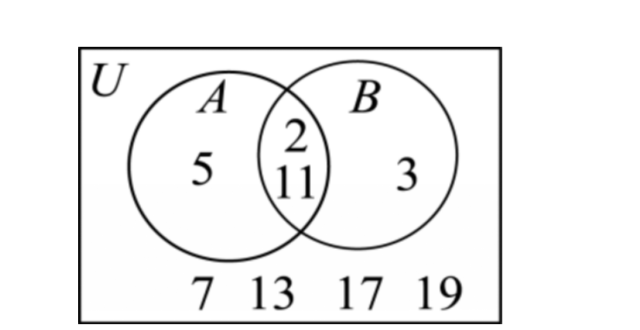
\includegraphics[width=0.24\textwidth]{figures/gao108_q6.png}
\end{center}

\solend
\fi

\item 若 $x\in A$，则 $\dfrac1x\in A$，就称 $A$ 自倒集合，集合 $M=\left\{-2,-1,0,\dfrac12,\dfrac13,1,2,3,4\right\}$ 的所有非空
子集中，自倒集合的个数为\blankline[4.4em].

\ifanswer
\solbegin
\step{由新定义，集合 $M$ 中的元素 1 和 $-1$ 倒数等于本身，2 和 $\dfrac12$，3 和 $\dfrac13$ 互为倒数,}
\step{故满足条件的自倒集合与集合 $\{-1,1,2,3\}$ 的非空子集的个数相同,}
\step{则其个数为 $2^4-1=15$.}
\solend
\fi

\item 设集合 $M=\{(x,y)\mid y=x^2+2bx+1\}$，$N=\{(x,y)\mid y=x+b\}(b\in\R)$，若
$M\cap N=\varnothing$，则实数 $b$ 的取值范围为\blankline[4.4em].

\ifanswer
\solbegin
\step{因为 $M\cap N=\varnothing$，所以
$\begin{cases}y=x^2+2bx+1\\y=x+b\end{cases}$
无解，则 $x^2+(2b-1)x+(1-b)=0$,}
\step{则 $\triangle=(2b-1)^2-4\times1\times(1-b)=4b^2-3<0$，解得 $-\dfrac{\sqrt3}2<b<\dfrac{\sqrt3}2$,}
\step{即实数 $b$ 的取值范围为 $\left(-\dfrac{\sqrt3}2,\dfrac{\sqrt3}2\right)$.}
\solend
\fi

\item 已知集合 $A=\left\{x\,\middle|\,\dfrac{x-a}{x^2-1}=1\right\}$ 有唯一元素，用列举法表示满足集合 $A$ 的条件的 $a$ 的取值集
合\blankline[4.4em].

\ifanswer
\solbegin
\step{$a=1$,$\dfrac{1}{x+1}=1$，一解；$a=-1$,$\dfrac{1}{x-1}=1$，一解；}
\step{$x-a=x^2-1$，一解时，$a=\dfrac54$,}
\step{综上，$a$ 的取值集合为 $\left\{-1,1,\dfrac54\right\}$.}
\solend
\fi

\item 已知集合 $M$ 的元素均为正整数，定义集合 $M$ 的“变项和”为：将 $M$ 中每个元素 $m$ 都乘
以 $(-1)^n$ 后再求和. 若集合 $A=\{n\mid1\leqslant n\leqslant2026,n\in\N\}$，则集合 $A$ 的所有非空子集的“变
项和”的总和为\blankline[4.4em].% $n$ 未加界定（据解析为元素序号），照录

\ifanswer
\solbegin
\step{$A=\{n\mid1\leqslant n\leqslant2026,n\in\N\}=\{1,2,\cdots,2026\}$,}
\step{1 在所有非空子集中共出现 $C_{2025}^{0}+C_{2025}^{1}+\cdots+C_{2025}^{2025}=2^{2025}$ 次,}
\step{同理 $2,3,\cdots,2026$ 都出现 $2^{2025}$ 次,}
\step{则集合 $A$ 的所有非空子集的“变项和”的总和}
\step{为 $2^{2025}\times[1\times(-1)^1+2\times(-1)^2+\cdots+2026\times(-1)^{2026}]$}
\step{$=2^{2025}\times(-1+2-3+4-\cdots-2025+2026)=1013\times2^{2025}$.}
\solend
\fi

\item 已知 $0<k<2$，定义 $[x]$ 为不超过 $x$ 的最大整数，区间 $[a,b]$（或 $(a,b)$，$[a,b)$，
$(a,b]$）的长度记为 $b-a$. 若关于 $x$ 的不等式 $k[x]>\lvert2[x]-6\rvert$ 的解集对应区间的长度为 $2$，
则 $k$ 的取值范围是\blankline[4.4em].

\ifanswer
\solbegin
\stepm{法一：}{由题意得 $\lvert2[x]-6\rvert=
\begin{cases}2[x]-6,x\geqslant3\\-2[x]+6,x<3\end{cases}$.}
\step{①当 $x\geqslant3$ 时，不等式 $k[x]>\lvert2[x]-6\rvert$ 可化为 $k[x]>2[x]-6$,}
\step{即 $(2-k)[x]<6$,}
\step{当 $0<k<2$ 时，解不等式 $(2-k)[x]<6$ 得 $[x]<\dfrac6{2-k}$.}
\step{②当 $x<3$ 时，不等式 $k[x]>\lvert2[x]-6\rvert$ 可化为 $k[x]>-2[x]+6$,}
\step{即 $(k+2)[x]>6$.}
\step{当 $0<k<2$ 时，解不等式 $(k+2)[x]>6$ 得 $[x]>\dfrac6{k+2}$.}
\step{综上所述，不等式 $k[x]>\lvert2[x]-6\rvert$ 的解集需满足 $\dfrac6{k+2}<[x]<\dfrac6{2-k}$,}
\step{由题意得在区间 $\left[\dfrac6{k+2},\dfrac6{2-k}\right]$ 内有两个整数,}
\step{由于 $\dfrac6{k+2}\in\left(\dfrac32,3\right)$，所以 $\dfrac6{2-k}\leqslant5$，得 $k\leqslant\dfrac45$.}
\step{因此 $k\in\left(0,\dfrac45\right]$，得 $\dfrac6{k+2}\in\left[\dfrac75,3\right)$，$\dfrac6{2-k}\in(3,5]$,}
\step{区间 $\left[\dfrac6{k+2},\dfrac6{2-k}\right]$ 内的两个整数是 3、4，所以 $4<\dfrac6{2-k}\leqslant5$，解得 $\dfrac12<k\leqslant\dfrac45$,}
\step{即 $k\in\left(\dfrac12,\dfrac45\right]$.}
\stepm{法二：}{令 $f(x)=kx$，$g(x)=\lvert2x-6\rvert$，画出 $g(x)$、$f(x)$ 的图象,}
\step{由于不等式 $k[x]>\lvert2[x]-6\rvert$ 的解集对应区间的长度为 2,}
\step{因此解集只可能为 $[3,5)$ 或 $[2,4)$.}
\step{当解集为 $[3,5)$ 时，如图（2），数形结合易得
$\begin{cases}f(2)\leqslant g(2)\\f(4)>g(4)\\f(5)\leqslant g(5)\end{cases}$,}
\step{即
$\begin{cases}2k\leqslant\lvert2\times2-6\rvert\\4k>\lvert2\times4-6\rvert\\5k\leqslant\lvert2\times5-6\rvert\end{cases}$，
解得
$\begin{cases}k\leqslant1\\k>\dfrac12\\k\leqslant\dfrac45\end{cases}$，
所以 $\dfrac12<k\leqslant\dfrac45$，满足 $0<k<2$,}
\step{当解集为 $[2,4)$ 时，如图（1），数形结合易得
$\begin{cases}f(2)>g(2)\\f(4)\leqslant g(4)\end{cases}$,}
\step{即
$\begin{cases}2k>\lvert2\times2-6\rvert\\4k\leqslant\lvert2\times4-6\rvert\end{cases}$，
无解.}

\begin{center}
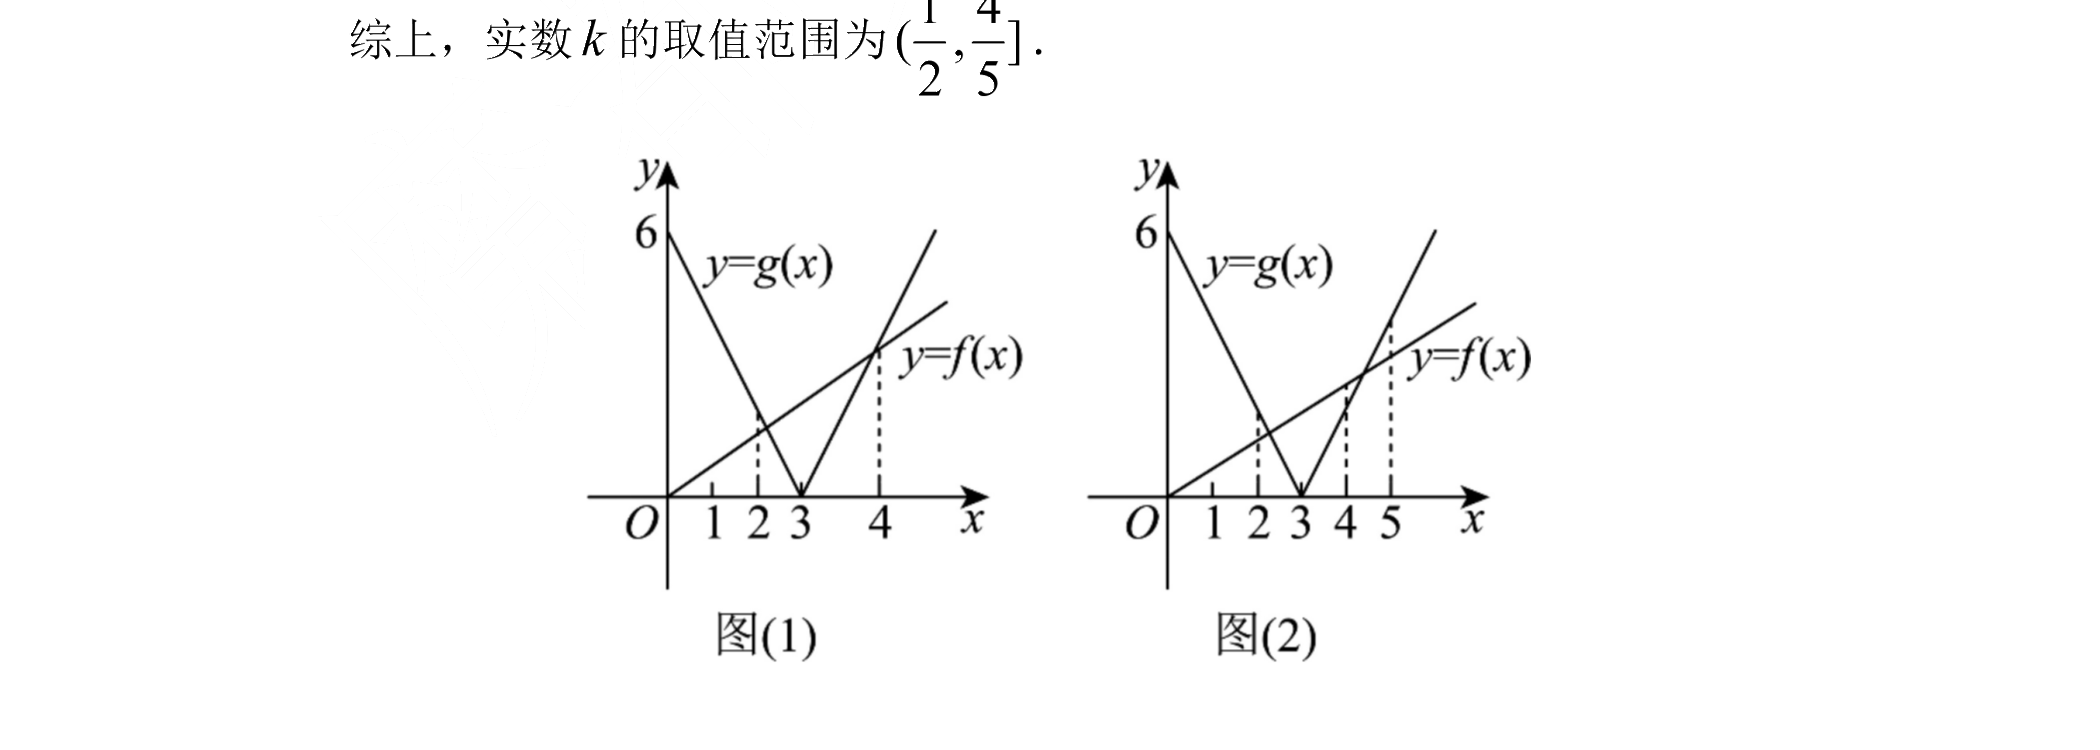
\includegraphics[width=0.72\textwidth]{figures/gao108_q11.png}
\end{center}

\step{综上，实数 $k$ 的取值范围为 $\left(\dfrac12,\dfrac45\right]$.}
\solend
\fi

\item 已知集合 $A=[1,a]\cup[a^3,a^4]$，集合 $B=\{x\mid x=x_1-x_2$，其中 $x_1$,$x_2\in A\}$. 若集合 $B$ 表
示的区间为一个闭区间，则实数 $a$ 的取值范围为\blankline[4.4em].

\ifanswer
\solbegin
\step{由题意得 $a^3>a>1$，则 $x_1-x_2$ 的最小值为 $1-a^4$，最大值为 $a^4-1$,}
\step{所以 $B=[1-a^4,a^4-1]$,}
\step{又因为 $a^4-a^3-(a-1)=a^3(a-1)-(a-1)=(a^3-1)(a-1)>0$,}
\step{所以 $a^4-a^3>a-1$，又集合 $B$ 表示的区间为一个闭区间,}
\step{则 $a^3-a\leqslant a^4-a^3$，化简得 $a^2-a-1\geqslant0$，又 $a>1$，解得 $a\geqslant\dfrac{1+\sqrt5}2$.}
\solend
\fi

\end{enumerate}

\bigsec{二、选择题}

\begin{enumerate}
\setcounter{enumi}{12}

\item 若 $a,b,c\in\R$，则下列不等式恒成立的是\mbox{（\quad）}% 原卷把答案“C”印在题干括号内、无【解析】

\keepwithprev
A. $\dfrac1a<\dfrac1b$\qquad B. $a^2<b^2$\qquad C. $\dfrac{a}{c^2+1}>\dfrac{b}{c^2+1}$\qquad D. $a\lvert c\rvert>b\lvert c\rvert$

\ifanswer
\ans{$C$}
\fi

\item 以下几个关系中正确的是\mbox{（\quad）}

\keepwithprev
A. $0\in\varnothing$\qquad\qquad\qquad B. $\varnothing\in\{x\mid x^2+1=0\}$

C. $\varnothing\subset\{0\}$\qquad\qquad\qquad D. $(A\cap B)\subset(A\cup B)$

\ifanswer
\solbegin
\step{$A$ 选项，$\varnothing$ 不包含任何元素，所以 $0\in\varnothing$ 错误，$A$ 错,}
\step{$B$ 选项，集合与集合之间关系不可以用 $\in$，$B$ 错,}
\step{$C$ 选项，空集是非空集合的真子集，所以 $\varnothing\subset\{0\}$ 正确，$C$ 对,}
\step{$D$ 选项，当 $A=B$ 时，$(A\cap B)=(A\cup B)$，$D$ 错,}
\step{故选 $C$.}
\solend
\fi

\item 设全集为 $U$，图中阴影部分所表示的集合是\mbox{（\quad）}% 原卷把答案“A”印在题干括号内、无【解析】

\keepwithprev
A. $B\cap\overline{A\cup C}$\qquad\qquad B. $(A\cup B)\cap(B\cup C)$

C. $(A\cup C)\cap\overline B$\qquad\qquad D. $(\overline A\cup\overline C)\cap B$

\ifanswer
\ans{$A$}
\fi

\item 对于 $k=0,1,2,\cdots$，定义集合 $A_k=\{20+k,26+2k\}$，并记 $S_k=A_0\cup A_1\cup\cdots\cup A_k$，则
使得集合 $S_n$ 中完全平方数的个数为奇数的最小正整数 $n$ 为\mbox{（\quad）}

\keepwithprev
A. $18$\qquad\qquad B. $19$\qquad\qquad C. $20$\qquad\qquad D. $21$

\ifanswer
\solbegin
\step{当 $k=0$ 时，$A_0=\{20,26\}$，对于 $k=0,1,2,\cdots$,}
\step{集合 $A_k$ 中最小的元素 $20>4^2$，若 $S_n$ 中完全平方数的个数为奇数，则 $n>4$,}
\step{（1）$20+k=5^2$ 时，$k=5$，$A_5=\{25,36\}$，此时 $S_5$ 中完全平方数为 $5^2$、$6^2$,}
\step{个数为 2;}
\step{$20+k=6^2$ 时，$k=16$，$A_{16}=\{36,58\}$，此时 $S_{16}$ 中完全平方数为 $5^2$、$6^2$,}
\step{个数为 2;}
\step{$20+k=7^2$ 时，$k=29$，$A_{29}=\{49,84\}$,}
\step{此时 $S_{29}$ 中完全平方数为 $5^2$、$6^2$、$7^2$、$8^2$，个数为 4;}
\step{$20+k=8^2$ 时，$k=44$，$A_{44}=\{64,114\}$,}
\step{此时 $S_{44}$ 中完全平方数为 $5^2$、$6^2$、$7^2$、$8^2$、$10^2$，个数为 5;}
\step{（2）因为 $k=0,1,2,\cdots,26+2k$ 一定为偶数,}
\step{所以 $26+2k=6^2$ 时，$k=5$，由上述分析得 $S_5$ 中完全平方数个数为 2;}
\step{$26+2k=8^2$ 时，$k=19$，$A_{19}=\{39,64\}$,}
\step{此时 $S_{19}$ 中完全平方数为 $5^2$、$6^2$、$8^2$，个数为 3.}
\step{综上，使集合 $S_n$ 中完全平方数的个数为奇数的最小正整数 $n=19$. 故选 $B$.}
\solend
\fi

\end{enumerate}

\bigsec{三、解答题}

\begin{enumerate}
\setcounter{enumi}{16}

\item 设全集 $U=\R$，集合 $A=\left\{x\,\middle|\,\dfrac{x-2}{x+2}\leqslant0\right\}$，$B=\{x\mid a\leqslant x<2a+1,a\in\R\}$，
$C=\{x\mid\lvert2x-1\rvert<5\}$.

（1）求集合 $A$、$\overline A\cup C$；

（2）若 $B\subseteq A$，求实数 $a$ 的取值范围.

\ifanswer
\solbegin
\ansspace*
\step{（1）不等式 $\dfrac{x-2}{x+2}\leqslant0$，等价于
$\begin{cases}(x-2)(x+2)\leqslant0\\x+2\neq0\end{cases}$，
解得 $\{x\mid-2<x\leqslant2\}$,}
\step{所以 $A=\{x\mid-2<x\leqslant2\}$，则 $\overline A=\{x\mid x\leqslant-2$ 或 $x>2\}$,}
\step{因为 $C=\{x\mid\lvert2x-1\rvert<5\}=\{x\mid-2<x<3\}$，所以 $\overline A\cup C=\R$；}
\step{（2）因为 $B\subseteq A$,}
\step{若 $B=\varnothing$，则 $a\geqslant2a+1$，解得 $a\leqslant-1$,}
\step{若 $B\neq\varnothing$，则
$\begin{cases}a<2a+1\\a>-2\\2a+1\leqslant2\end{cases}$，
解得 $-1<a\leqslant\dfrac12$,}
\step{综上所述，实数 $a$ 的取值范围为 $\left\{a\,\middle|\,a\leqslant\dfrac12\right\}$.}
\solend
\fi

\item 设 $a$、$b$、$c$、$d$ 是四个正数.

（1）已知 $a>b$，比较 $\dfrac{2a+b}{a+2b}$ 与 $\dfrac ab$ 的值的大小；

（2）若 $(1+a)(1+b)(1+c)(1+d)<16$，求证：$a$、$b$、$c$、$d$ 中至少有一个小于 1.

\ifanswer
\solbegin
\step{（1）$\dfrac{2a+b}{a+2b}-\dfrac ab=\dfrac{b^2-a^2}{b(a+2b)}<0$，所以 $\dfrac{2a+b}{a+2b}<\dfrac ab$.}
\step{（2）假设 $a$、$b$、$c$、$d$ 都不小于 1，即 $a$、$b$、$c$、$d$ 均大于等于 1,}
\step{即 $a\geqslant1$，$b\geqslant1$，$c\geqslant1$，$d\geqslant1$,}
\step{由均值不等式得 $1+a\geqslant2\sqrt a$,$1+b\geqslant2\sqrt b$,$1+c\geqslant2\sqrt c$,$1+d\geqslant2\sqrt d$,}
\step{故 $(1+a)(1+b)(1+c)(1+d)\geqslant16\sqrt{abcd}\geqslant16$,}
\step{当且仅当 $a=b=c=d=1$ 时取等号,}
\step{这与 $(1+a)(1+b)(1+c)(1+d)<16$ 矛盾，故假设不成立，原命题成立.}
\solend
\fi

\item 已知 $m\in\R$，一个二次项系数为 1 的一元二次方程的两个不等实根分别为 $x_1$ 和 $x_2$，且
满足
$\begin{cases}x_1^2+x_2^2=2m^2-4\\x_1+x_2=m\end{cases}$.

（1）直接写出该一元二次方程；

（2）若 $(3x_1-x_2)(3x_2-x_1)\geqslant-1$，求 $m$ 的取值范围；

（3）若方程的两根 $x_1$ 和 $x_2$ 都大于 $-1$，求 $m$ 的取值范围.

\ifanswer
\solbegin
\step{（1）设这个一元二次方程为 $x^2+bx+c=0$,}
\step{由
$\begin{cases}x_1^2+x_2^2=2m^2-4\\x_1+x_2=m\end{cases}$,}
\step{得 $(x_1+x_2)^2=x_1^2+x_2^2+2x_1x_2=2m^2-4+2x_1x_2=m^2$，即 $x_1x_2=\dfrac{4-m^2}2$,}
\step{由韦达定理得 $x_1+x_2=-b=m$，即 $x_1x_2=c=\dfrac{4-m^2}2$,}
\step{所以一元二次方程为 $x^2-mx+\dfrac{4-m^2}2=0$.}
\step{（2）$(3x_1-x_2)(3x_2-x_1)=9x_1x_2-3x_1^2-3x_2^2+x_1x_2=10x_1x_2-3(x_1^2+x_2^2)\geqslant-1$,}
\step{结合已知及（1）得 $x_1^2+x_2^2=2m^2-4$,$x_1x_2=\dfrac{4-m^2}2$,}
\step{代入得 $10\times\dfrac{4-m^2}2-3(2m^2-4)=-11m^2+32\geqslant-1\Rightarrow m^2\leqslant3$}
\step{$\Rightarrow-\sqrt3\leqslant m\leqslant\sqrt3$,}
\step{又 $\Delta=m^2-4\times\dfrac{4-m^2}2=3m^2-8>0\Rightarrow m<-\dfrac{2\sqrt6}3$ 或 $m>\dfrac{2\sqrt6}3$,}
\step{所以 $m\in\left[-\sqrt3,-\dfrac{2\sqrt6}3\right)\cup\left(\dfrac{2\sqrt6}3,\sqrt3\right]$.}
\step{（3）若方程的两根 $x_1$ 和 $x_2$ 都大于 $-1$，则
$\begin{cases}\Delta>0\\x_1+x_2>-2\\(x_1+1)(x_2+1)>0\end{cases}$,}
\step{所以
$\begin{cases}\Delta=3m^2-8>0\\m>-2\\[2pt]\dfrac{4-m^2}2+m+1>0\end{cases}$，
解得 $m\in\left(1-\sqrt7,-\dfrac{2\sqrt6}3\right)\cup\left(\dfrac{2\sqrt6}3,1+\sqrt7\right)$.}
\solend
\fi

\item 已知不等式 $2\leqslant ax^2+bx+c\leqslant3$ 的解集为 $\{x\mid2\leqslant x\leqslant3\}$.

（1）若 $a>0$，求 $6b+5c$ 的值；

（2）若 $a>0$，且不等式 $ax^2+(b-3)x-c\leqslant0$ 有且仅有 9 个整数解，求 $a$ 的取值范围；

（3）若 $a<0$，对任意的 $x<0$，不等式 $(ax-4)(x^2+b+c+1)\geqslant0$ 恒成立，求 $a^2-b+c$
的取值集合.

\ifanswer
\solbegin
\ansspace*
\step{（1）$a>0$,}
\step{结合二次函数图象得不等式 $ax^2+bx+c\leqslant3$ 的解集为 $\{x\mid2\leqslant x\leqslant3\}$,}
\step{且不等式 $ax^2+bx+c\geqslant2$ 的解集为 $R$,}
\step{所以方程 $ax^2+bx+c-3=0$ 的两根分别为 2 和 3,}
\step{则
$\begin{cases}2+3=-\dfrac ba\\[2pt]2\times3=\dfrac{c-3}a\end{cases}$，
得 $b=-5a$，$c=6a+3$,}
\step{所以 $6b+5c=6\times(-5a)+5(6a+3)=15$.}
\step{（2）若 $a>0$，且不等式 $ax^2+(b-3)x-c\leqslant0$ 有且仅有 9 个整数解,}
\step{由（1）得 $b=-5a$，$c=6a+3$,}
\step{不等式 $ax^2+bx+c\geqslant2$ 可化为 $ax^2-5ax+6a+1\geqslant0$.}
\step{由（1）得不等式 $ax^2+bx+c\geqslant2$ 的解集为 $R$,}
\step{所以 $ax^2-5ax+6a+1\geqslant0$ 恒成立,}
\step{所以
$\begin{cases}a>0\\\Delta=25a^2-4a(6a+1)\leqslant0\end{cases}$，
即
$\begin{cases}a>0\\a^2-4a=a(a-4)\leqslant0\end{cases}$，}
\step{解得 $0<a\leqslant4$.}
\step{不等式 $ax^2+(b-3)x-c\leqslant0$ 等价于 $ax^2-(5a+3)x-(6a+3)\leqslant0$,}
\step{所以 $[ax-(6a+3)](x+1)\leqslant0$，得 $-1\leqslant x\leqslant6+\dfrac3a$,}
\step{所以 $7\leqslant6+\dfrac3a<8$，解得 $\dfrac32<a\leqslant3$.}
\step{综上，$a$ 的取值范围为 $\left(\dfrac32,3\right]$.}
\step{（3）因为 $a<0$,}
\step{同（1）分析，不等式 $ax^2+bx+c\geqslant2$ 的解集为 $\{x\mid2\leqslant x\leqslant3\}$,}
\step{$ax^2+bx+c\leqslant3$ 的解集为 $R$,}
\step{所以方程 $ax^2+bx+c-2=0$ 的两根分别为 2 和 3,}
\step{则
$\begin{cases}2+3=-\dfrac ba\\[2pt]2\times3=\dfrac{c-2}a\end{cases}$，
得 $b=-5a$，$c=6a+2$.}
\step{所以不等式 $ax^2+bx+c=ax^2-5ax+6a+2\leqslant3$ 的解集为 $R$,}
\step{则 $ax^2-5ax+6a-1\leqslant0$ 恒成立,}
\step{所以
$\begin{cases}a<0\\\Delta=25a^2-4a(6a-1)\leqslant0\end{cases}$，
即
$\begin{cases}a<0\\a^2+4a=a(a+4)\leqslant0\end{cases}$，}
\step{解得 $-4\leqslant a<0$.}
\step{所以对任意的 $x<0$，不等式 $(ax-4)(x^2+b+c+1)\geqslant0$ 恒成立}
\step{转化为对任意的 $x<0$，不等式 $(ax-4)(x^2+a+3)\geqslant0$ 恒成立.}
\step{方程 $(ax-4)(x^2+a+3)=0$ 的两个根为 $x=\dfrac4a<0$,}
\step{$x=\pm\sqrt{-a-3}$（$a<-3$ 时成立）,}
\step{因而仅当 $ax-4=0$ 与 $x^2+a+3=0$ 的负根重合时满足条件,}
\step{解得唯一解为 $a=-4$，所以 $a^2-b+c=a^2+11a+2=-26$,}
\step{所以 $a^2-b+c$ 的取值集合为 $\{-26\}$.}
\solend
\fi

\item 已知集合 $A=\{1,2,3,4,5,6,7,8\}$，$M=\{(x,y)\mid x\in A,y\in A\}$，从 $M$ 中选取 $n$ 个不同的
元素组成一个序列：$(x_1,y_1)$,$(x_2,y_2),\cdots,(x_n,y_n)$，其中 $(x_i,y_i)$ 称为该序列的第 $i$ 项
（$i=1,2,\cdots,n$），若该序列的相邻项 $(x_i,y_i)$,$(x_{i+1},y_{i+1})$ 满足：
\[\begin{cases}\lvert x_{i+1}-x_i\rvert=3\\\lvert y_{i+1}-y_i\rvert=4\end{cases}
\quad\text{或}\quad
\begin{cases}\lvert x_{i+1}-x_i\rvert=4\\\lvert y_{i+1}-y_i\rvert=3\end{cases}\]
（$i=1,2,\cdots,n-1$），则称该序列为“$\Delta-$序列”.

（1）若一个 $\Delta-$序列的第一项为 $(4,4)$，请直接写出它所有可能的第二项；

（2）定义集合 $A=\{1,2,3,4,5,6,7,8\}$ 的两个子集：外侧集 $S=\{1,2,7,8\}$，内侧集
$T=\{3,4,5,6\}$. 证明：若 $\Delta-$序列中某一项的坐标在区域 $S\times S$ 内（即横、纵坐标均属于
$S$），则它的下一项坐标必定在区域 $T\times T$ 内；

（3）证明：不存在一个恰好有 5 项的 $\Delta-$序列，使其第一项为 $(1,8)$，且第五项为
$(8,1)$.

\ifanswer
\solbegin
\ansspace*
\step{（1）由题意，第一项为 $(x_1,y_1)=(4,4)$,}
\step{对于第二项 $(x_2,y_2)$，其坐标必须在 1~8 之间.}
\step{若 $\lvert x_2-4\rvert=3$,$\lvert y_2-4\rvert=4$，则 $x_2\in\{1,7\}$,}
\step{且 $y_2\in\{8\}$（因为 $4-4=0$ 不在集合 $A$ 中）. 此时可能的点为 $(1,8)$,$(7,8)$.}
\step{若 $\lvert x_2-4\rvert=4$,$\lvert y_2-4\rvert=3$，则 $x_2\in\{8\}$，且 $y_2\in\{1,7\}$.}
\step{此时可能的点为 $(8,1)$,$(8,7)$.}
\step{所以它所有可能的第二项为 $(1,8)$,$(7,8)$,$(8,1)$,$(8,7)$.}
\step{（2）已知某一项 $(x_t,y_t)\in S\times S$，即 $x_t\in\{1,2,7,8\}$ 且 $y_t\in\{1,2,7,8\}$.}
\step{由规则得下一步坐标的变化量为 3 和 4，设 $a\in S$ 变化 3 或 4 后的结果 $a'$:}
\step{当 $a=1$ 时，$1+3=4\in T$,$1+4=5\in T$；}
\step{当 $a=2$ 时，$2+3=5\in T$,$2+4=6\in T$；}
\step{当 $a=7$ 时，$7-3=4\in T$,$7-4=3\in T$；}
\step{当 $a=8$ 时，$8-3=5\in T$,$8-4=4\in T$.}
\step{（注：由于超出 1~8 范围的越界坐标不符合.）}
\step{由此可见，无论 $a$ 是 $S$ 中的哪一个数，加上或减去 3 或 4 之后,}
\step{得到的新坐标必属于集合 $T$.}
\step{因为 $\Delta-$序列每走一步，横坐标和纵坐标必定同时发生 3 和 4 的变化,}
\step{所以新的横坐标 $x_{i+1}$ 必属于 $T$，新的纵坐标 $y_{i+1}$ 也必属于 $T$,}
\step{即下一项 $(x_{i+1},y_{i+1})$ 必定在区域 $T\times T$ 内. ………10 分原命题得证.% 得分行混入证明，照录
}
\step{（3）假设存在这样一个包含 5 项的 $\Delta-$序列:}
\step{$(x_1,y_1)$,$(x_2,y_2)$,$(x_3,y_3)$,$(x_4,y_4)$,$(x_5,y_5)$.}
\step{已知第一项为 $(1,8)$，第五项为 $(8,1)$. 第 2 项必须是第 1 项 $(1,8)$ 的相邻点.}
\step{我们来找 $(1,8)$ 的相邻点：第 2 项只能是 $(4,4)$ 或 $(5,5)$,}
\step{第 4 项必须是第 5 项 $(8,1)$ 的相邻点（因为跳跃是双向可逆的）.}
\step{同理可算得，$(8,1)$ 的相邻点也只有两个：$(4,4)$ 和 $(5,5)$,}
\step{题目题干中明确规定，$\Delta-$序列由 $n$ 个不同的有序数对构成.% “题目题干”措辞重复，照录
}
\step{所以，第 2 项和第 4 项不能是同一个点. 这就意味着:}
\step{如果第 2 项是 $(4,4)$，第 4 项就必须是 $(5,5)$；反之亦然.}
\step{则第 3 项必须是 $(4,4)$ 和 $(5,5)$ 的公共相邻点.}
\step{$(4,4)$ 的相邻点集合为：$\{(1,8),(7,8),(8,1),(8,7)\}$,}
\step{$(5,5)$ 的相邻点集合为：$\{(2,1),(8,1),(1,2),(1,8)\}$,}
\step{所以，第 3 项只能填 $(1,8)$ 或者 $(8,1)$.}
\step{这与“序列由不同的有序数对构成”这一条件产生矛盾！}
\step{所以，不存在一个恰好有 5 项的 $\Delta-$序列,}
\step{使其第一项为 $(1,8)$，且第五项为 $(8,1)$.}
\solend
\fi

\end{enumerate}

\end{document}
"
%
% 原始材料：微信公众号“魔都数学加油站”文章，作者破晓，2026-11-03 17:19 发布；
% 连载“27学年高一108”，原文标题“27学年高一108——2026-2027年上海市五校联考高一上10月月考”；
% 原文链接：https://mp.weixin.qq.com/s/3nkP789Qar93NGMZXFFCSw。
% 正文为 14 张 PNG 页（第 2、3、6—13 页 4762×6735，第 1、4、5、14 页 2560×3620），
% 题目下印有【解析】，为讲评版。
% 题目、解析均据原图转录；卷面水印及公众号页脚未录入。
% 第 6 题解析的文氏图与第 11 题法二解析的两幅图象（图(1)、图(2)）裁自原图、去粉色水印
% 转灰度（gao108_q6.png、gao108_q11.png），第 6 题图属解析（仅答案版）、
% 第 11 题图属解析（仅答案版）。
%
% 卷首标题：原卷印作“2026-2027 年五校联考高一上 10 月月考”，标题下另印一行参与学校
% 名单“闵行中学、嘉定一中、松江一中、金山中学、嘉一实高”（全稿第 5 份原卷自印副标题，
% 按 14／24／49／50 成例照录，并登记进计数核对.py 的 SELFSUB）。
%
% 与原卷的排版差异：
%   ① 原文从第 3 题起，填空题编号为 3—12、选择题为 13—16、解答题为 17—21，本稿保留原题号；
%   ② 原卷每题下直接印【解析】，本稿按全稿惯例将解析置于答案版；第 4 题只印【答案】，
%      第 13、15 两题把答案印在题干括号内且无【解析】，均另提 \ans{}；
%   ③ 原卷副标题照录（见上）；
%   ④ 原卷填空横线按全稿惯例排为 \blankline[4.4em]；解答题按惯例加 \ansspace；选择题括号排
%      \mbox{（\quad）}、选项段前按惯例加 \keepwithprev；
%   ⑤ 原卷数集排斜体 $R$／$N$，按全稿惯例改 \R、\N。
%
% 原卷红色强调照录为黑体：第 11 题解析的“法一：”“法二：”原卷排红色，按 53 成例排
% \stepm{法一：}／\stepm{法二：}（加粗着色）。
%
% 原卷存疑：第 10 题题干“变项和”定义中“将 $M$ 中每个元素 $m$ 都乘以 $(-1)^n$ 后再求和”
% 的 $n$ 未加界定（据解析应为该元素在 $\{1,2,\cdots,2026\}$ 中的序号），照录。
% 第 21 题 (2) 解析末行“即下一项 $(x_{i+1},y_{i+1})$ 必定在区域 $T\times T$ 内. ………10 分
% 原命题得证.”，原卷把得分点行混入证明（“原命题”按上下文为“原命题的逆否”），照录。
% 第 21 题 (3) 解析“题目题干中明确规定”，“题目题干”措辞重复，照录。
%
% 行数核对：逐题数 \step/\stepm 条数，合计 164 条（Q3：3；Q4：0；Q5：2；Q6：1；Q7：3；
% Q8：3；Q9：3；Q10：6；Q11：21；Q12：5；Q13：0；Q14：5；Q15：0；Q16：15；Q17：7；
% Q18：7；Q19：13；Q20：34；Q21：36），与原卷印刷行逐题相等。第 4 题只印【答案】、
% 第 13、15 题括号内印答案，均提 \ans{}，不计入 \step 账。
%
\documentclass[a4paper,11pt]{article}
\usepackage{common}

\begin{document}

\examtitlest[3]{2026--2027 年五校联考高一上 10 月月考}{闵行中学、嘉定一中、松江一中、金山中学、嘉一实高}

\bigsec{一、填空题}

\begin{enumerate}
\setcounter{enumi}{2}

\item 已知等式 $2x^2+3x+5=2ax^2+a(3x+1)+c$ 恒成立，则实数 $a+c$ 的值为\blankline[4.4em].

\ifanswer
\solbegin
\step{因为 $2x^2+3x+5=2ax^2+a(3x+1)+c$ 恒成立,}
\step{即 $2x^2+3x+5=2ax^2+3ax+(a+c)$ 恒成立，所以
$\begin{cases}2=2a\\3=3a\\5=a+c\end{cases}$,}
\step{所以 $a+c=5$.}
\solend
\fi

\item 不等式 $\dfrac1x<\dfrac12$ 的解集是\blankline[4.4em].

\ifanswer
\ans{$(-\infty,0)\cup(2,+\infty)$}
\fi

\item 已知 $a$、$b$ 都是实数，则“$a^2=b^2$”是“$a^2+b^2=2ab$”的\blankline[4.4em]条件.

\ifanswer
\solbegin
\step{$a^2=b^2$ 等价于 $a=\pm b$；$a^2+b^2=2ab$ 等价于 $(a-b)^2=0$ 等价于 $a=b$,}
\step{故“$a^2=b^2$”是“$a^2+b^2=2ab$”的必要不充分条件.}
\solend
\fi

\item 已知全集 $U=\{x\mid x$ 为不大于 20 的素数$\}$，$A\cap\overline B=\{5\}$，$\overline A\cap B=\{3\}$，
$\overline{A\cup B}=\{7,13,17,19\}$，则 $A=$\blankline[4.4em].

\ifanswer
\solbegin
\step{如图所示，$A=\{2,5,11\}$.}

\begin{center}
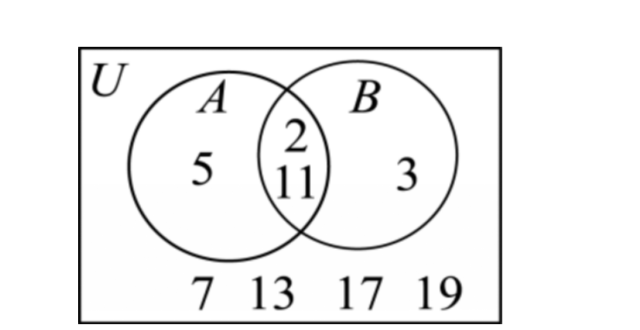
\includegraphics[width=0.24\textwidth]{figures/gao108_q6.png}
\end{center}

\solend
\fi

\item 若 $x\in A$，则 $\dfrac1x\in A$，就称 $A$ 自倒集合，集合 $M=\left\{-2,-1,0,\dfrac12,\dfrac13,1,2,3,4\right\}$ 的所有非空
子集中，自倒集合的个数为\blankline[4.4em].

\ifanswer
\solbegin
\step{由新定义，集合 $M$ 中的元素 1 和 $-1$ 倒数等于本身，2 和 $\dfrac12$，3 和 $\dfrac13$ 互为倒数,}
\step{故满足条件的自倒集合与集合 $\{-1,1,2,3\}$ 的非空子集的个数相同,}
\step{则其个数为 $2^4-1=15$.}
\solend
\fi

\item 设集合 $M=\{(x,y)\mid y=x^2+2bx+1\}$，$N=\{(x,y)\mid y=x+b\}(b\in\R)$，若
$M\cap N=\varnothing$，则实数 $b$ 的取值范围为\blankline[4.4em].

\ifanswer
\solbegin
\step{因为 $M\cap N=\varnothing$，所以
$\begin{cases}y=x^2+2bx+1\\y=x+b\end{cases}$
无解，则 $x^2+(2b-1)x+(1-b)=0$,}
\step{则 $\triangle=(2b-1)^2-4\times1\times(1-b)=4b^2-3<0$，解得 $-\dfrac{\sqrt3}2<b<\dfrac{\sqrt3}2$,}
\step{即实数 $b$ 的取值范围为 $\left(-\dfrac{\sqrt3}2,\dfrac{\sqrt3}2\right)$.}
\solend
\fi

\item 已知集合 $A=\left\{x\,\middle|\,\dfrac{x-a}{x^2-1}=1\right\}$ 有唯一元素，用列举法表示满足集合 $A$ 的条件的 $a$ 的取值集
合\blankline[4.4em].

\ifanswer
\solbegin
\step{$a=1$,$\dfrac{1}{x+1}=1$，一解；$a=-1$,$\dfrac{1}{x-1}=1$，一解；}
\step{$x-a=x^2-1$，一解时，$a=\dfrac54$,}
\step{综上，$a$ 的取值集合为 $\left\{-1,1,\dfrac54\right\}$.}
\solend
\fi

\item 已知集合 $M$ 的元素均为正整数，定义集合 $M$ 的“变项和”为：将 $M$ 中每个元素 $m$ 都乘
以 $(-1)^n$ 后再求和. 若集合 $A=\{n\mid1\leqslant n\leqslant2026,n\in\N\}$，则集合 $A$ 的所有非空子集的“变
项和”的总和为\blankline[4.4em].% $n$ 未加界定（据解析为元素序号），照录

\ifanswer
\solbegin
\step{$A=\{n\mid1\leqslant n\leqslant2026,n\in\N\}=\{1,2,\cdots,2026\}$,}
\step{1 在所有非空子集中共出现 $C_{2025}^{0}+C_{2025}^{1}+\cdots+C_{2025}^{2025}=2^{2025}$ 次,}
\step{同理 $2,3,\cdots,2026$ 都出现 $2^{2025}$ 次,}
\step{则集合 $A$ 的所有非空子集的“变项和”的总和}
\step{为 $2^{2025}\times[1\times(-1)^1+2\times(-1)^2+\cdots+2026\times(-1)^{2026}]$}
\step{$=2^{2025}\times(-1+2-3+4-\cdots-2025+2026)=1013\times2^{2025}$.}
\solend
\fi

\item 已知 $0<k<2$，定义 $[x]$ 为不超过 $x$ 的最大整数，区间 $[a,b]$（或 $(a,b)$，$[a,b)$，
$(a,b]$）的长度记为 $b-a$. 若关于 $x$ 的不等式 $k[x]>\lvert2[x]-6\rvert$ 的解集对应区间的长度为 $2$，
则 $k$ 的取值范围是\blankline[4.4em].

\ifanswer
\solbegin
\stepm{法一：}{由题意得 $\lvert2[x]-6\rvert=
\begin{cases}2[x]-6,x\geqslant3\\-2[x]+6,x<3\end{cases}$.}
\step{①当 $x\geqslant3$ 时，不等式 $k[x]>\lvert2[x]-6\rvert$ 可化为 $k[x]>2[x]-6$,}
\step{即 $(2-k)[x]<6$,}
\step{当 $0<k<2$ 时，解不等式 $(2-k)[x]<6$ 得 $[x]<\dfrac6{2-k}$.}
\step{②当 $x<3$ 时，不等式 $k[x]>\lvert2[x]-6\rvert$ 可化为 $k[x]>-2[x]+6$,}
\step{即 $(k+2)[x]>6$.}
\step{当 $0<k<2$ 时，解不等式 $(k+2)[x]>6$ 得 $[x]>\dfrac6{k+2}$.}
\step{综上所述，不等式 $k[x]>\lvert2[x]-6\rvert$ 的解集需满足 $\dfrac6{k+2}<[x]<\dfrac6{2-k}$,}
\step{由题意得在区间 $\left[\dfrac6{k+2},\dfrac6{2-k}\right]$ 内有两个整数,}
\step{由于 $\dfrac6{k+2}\in\left(\dfrac32,3\right)$，所以 $\dfrac6{2-k}\leqslant5$，得 $k\leqslant\dfrac45$.}
\step{因此 $k\in\left(0,\dfrac45\right]$，得 $\dfrac6{k+2}\in\left[\dfrac75,3\right)$，$\dfrac6{2-k}\in(3,5]$,}
\step{区间 $\left[\dfrac6{k+2},\dfrac6{2-k}\right]$ 内的两个整数是 3、4，所以 $4<\dfrac6{2-k}\leqslant5$，解得 $\dfrac12<k\leqslant\dfrac45$,}
\step{即 $k\in\left(\dfrac12,\dfrac45\right]$.}
\stepm{法二：}{令 $f(x)=kx$，$g(x)=\lvert2x-6\rvert$，画出 $g(x)$、$f(x)$ 的图象,}
\step{由于不等式 $k[x]>\lvert2[x]-6\rvert$ 的解集对应区间的长度为 2,}
\step{因此解集只可能为 $[3,5)$ 或 $[2,4)$.}
\step{当解集为 $[3,5)$ 时，如图（2），数形结合易得
$\begin{cases}f(2)\leqslant g(2)\\f(4)>g(4)\\f(5)\leqslant g(5)\end{cases}$,}
\step{即
$\begin{cases}2k\leqslant\lvert2\times2-6\rvert\\4k>\lvert2\times4-6\rvert\\5k\leqslant\lvert2\times5-6\rvert\end{cases}$，
解得
$\begin{cases}k\leqslant1\\k>\dfrac12\\k\leqslant\dfrac45\end{cases}$，
所以 $\dfrac12<k\leqslant\dfrac45$，满足 $0<k<2$,}
\step{当解集为 $[2,4)$ 时，如图（1），数形结合易得
$\begin{cases}f(2)>g(2)\\f(4)\leqslant g(4)\end{cases}$,}
\step{即
$\begin{cases}2k>\lvert2\times2-6\rvert\\4k\leqslant\lvert2\times4-6\rvert\end{cases}$，
无解.}

\begin{center}
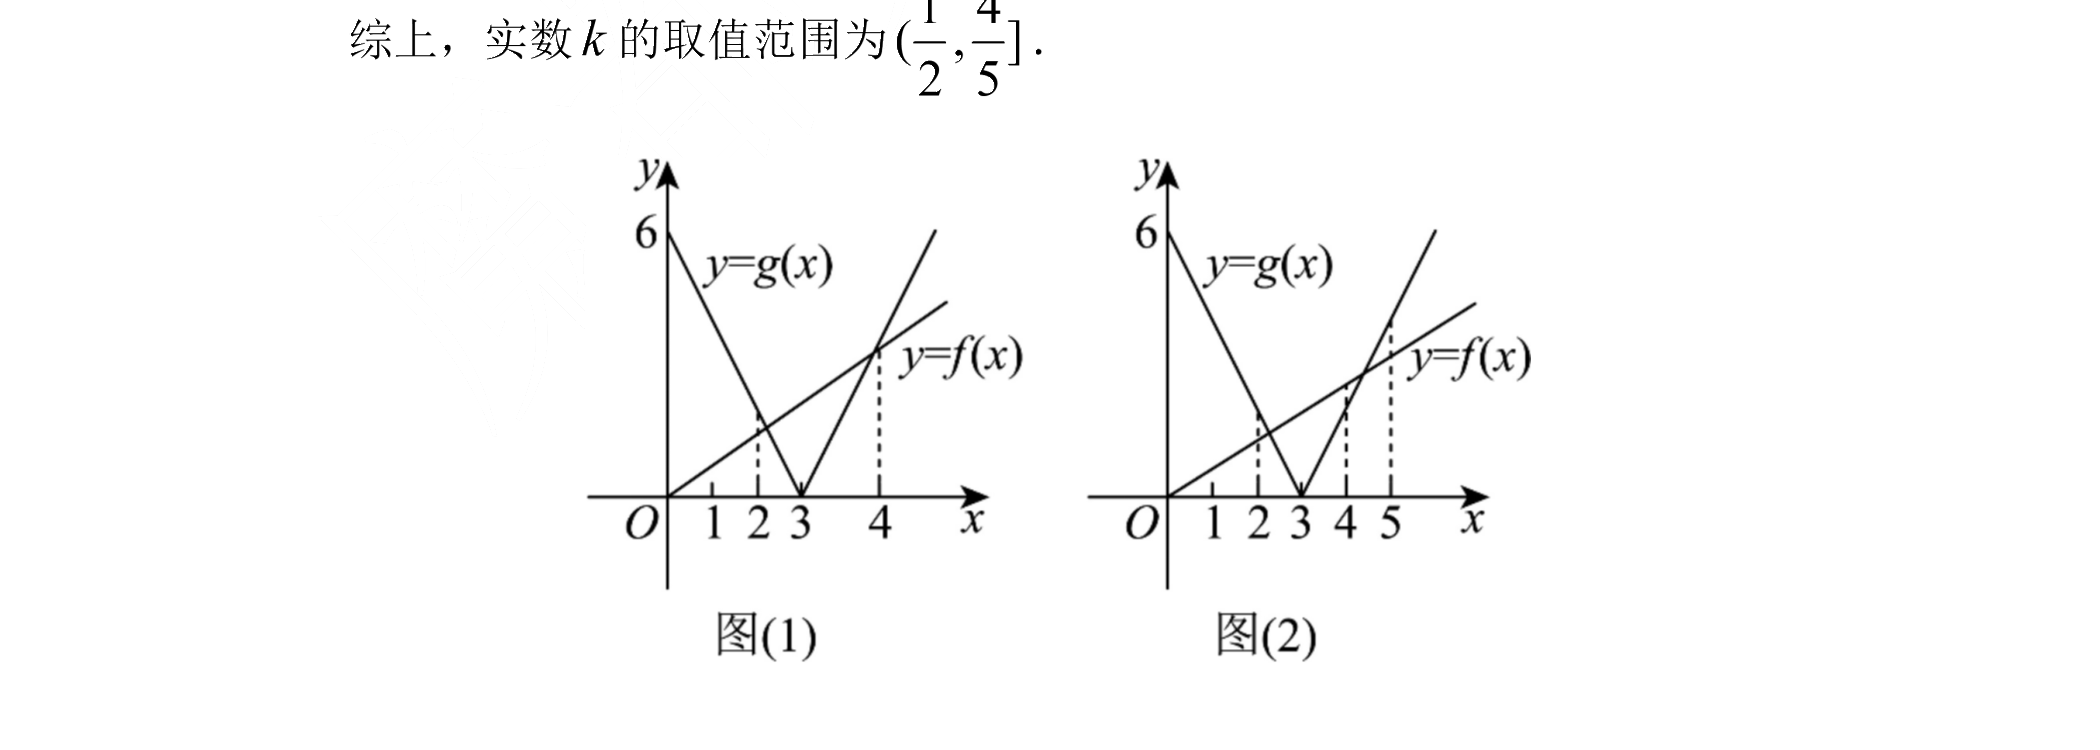
\includegraphics[width=0.72\textwidth]{figures/gao108_q11.png}
\end{center}

\step{综上，实数 $k$ 的取值范围为 $\left(\dfrac12,\dfrac45\right]$.}
\solend
\fi

\item 已知集合 $A=[1,a]\cup[a^3,a^4]$，集合 $B=\{x\mid x=x_1-x_2$，其中 $x_1$,$x_2\in A\}$. 若集合 $B$ 表
示的区间为一个闭区间，则实数 $a$ 的取值范围为\blankline[4.4em].

\ifanswer
\solbegin
\step{由题意得 $a^3>a>1$，则 $x_1-x_2$ 的最小值为 $1-a^4$，最大值为 $a^4-1$,}
\step{所以 $B=[1-a^4,a^4-1]$,}
\step{又因为 $a^4-a^3-(a-1)=a^3(a-1)-(a-1)=(a^3-1)(a-1)>0$,}
\step{所以 $a^4-a^3>a-1$，又集合 $B$ 表示的区间为一个闭区间,}
\step{则 $a^3-a\leqslant a^4-a^3$，化简得 $a^2-a-1\geqslant0$，又 $a>1$，解得 $a\geqslant\dfrac{1+\sqrt5}2$.}
\solend
\fi

\end{enumerate}

\bigsec{二、选择题}

\begin{enumerate}
\setcounter{enumi}{12}

\item 若 $a,b,c\in\R$，则下列不等式恒成立的是\mbox{（\quad）}% 原卷把答案“C”印在题干括号内、无【解析】

\keepwithprev
A. $\dfrac1a<\dfrac1b$\qquad B. $a^2<b^2$\qquad C. $\dfrac{a}{c^2+1}>\dfrac{b}{c^2+1}$\qquad D. $a\lvert c\rvert>b\lvert c\rvert$

\ifanswer
\ans{$C$}
\fi

\item 以下几个关系中正确的是\mbox{（\quad）}

\keepwithprev
A. $0\in\varnothing$\qquad\qquad\qquad B. $\varnothing\in\{x\mid x^2+1=0\}$

C. $\varnothing\subset\{0\}$\qquad\qquad\qquad D. $(A\cap B)\subset(A\cup B)$

\ifanswer
\solbegin
\step{$A$ 选项，$\varnothing$ 不包含任何元素，所以 $0\in\varnothing$ 错误，$A$ 错,}
\step{$B$ 选项，集合与集合之间关系不可以用 $\in$，$B$ 错,}
\step{$C$ 选项，空集是非空集合的真子集，所以 $\varnothing\subset\{0\}$ 正确，$C$ 对,}
\step{$D$ 选项，当 $A=B$ 时，$(A\cap B)=(A\cup B)$，$D$ 错,}
\step{故选 $C$.}
\solend
\fi

\item 设全集为 $U$，图中阴影部分所表示的集合是\mbox{（\quad）}% 原卷把答案“A”印在题干括号内、无【解析】

\keepwithprev
A. $B\cap\overline{A\cup C}$\qquad\qquad B. $(A\cup B)\cap(B\cup C)$

C. $(A\cup C)\cap\overline B$\qquad\qquad D. $(\overline A\cup\overline C)\cap B$

\ifanswer
\ans{$A$}
\fi

\item 对于 $k=0,1,2,\cdots$，定义集合 $A_k=\{20+k,26+2k\}$，并记 $S_k=A_0\cup A_1\cup\cdots\cup A_k$，则
使得集合 $S_n$ 中完全平方数的个数为奇数的最小正整数 $n$ 为\mbox{（\quad）}

\keepwithprev
A. $18$\qquad\qquad B. $19$\qquad\qquad C. $20$\qquad\qquad D. $21$

\ifanswer
\solbegin
\step{当 $k=0$ 时，$A_0=\{20,26\}$，对于 $k=0,1,2,\cdots$,}
\step{集合 $A_k$ 中最小的元素 $20>4^2$，若 $S_n$ 中完全平方数的个数为奇数，则 $n>4$,}
\step{（1）$20+k=5^2$ 时，$k=5$，$A_5=\{25,36\}$，此时 $S_5$ 中完全平方数为 $5^2$、$6^2$,}
\step{个数为 2;}
\step{$20+k=6^2$ 时，$k=16$，$A_{16}=\{36,58\}$，此时 $S_{16}$ 中完全平方数为 $5^2$、$6^2$,}
\step{个数为 2;}
\step{$20+k=7^2$ 时，$k=29$，$A_{29}=\{49,84\}$,}
\step{此时 $S_{29}$ 中完全平方数为 $5^2$、$6^2$、$7^2$、$8^2$，个数为 4;}
\step{$20+k=8^2$ 时，$k=44$，$A_{44}=\{64,114\}$,}
\step{此时 $S_{44}$ 中完全平方数为 $5^2$、$6^2$、$7^2$、$8^2$、$10^2$，个数为 5;}
\step{（2）因为 $k=0,1,2,\cdots,26+2k$ 一定为偶数,}
\step{所以 $26+2k=6^2$ 时，$k=5$，由上述分析得 $S_5$ 中完全平方数个数为 2;}
\step{$26+2k=8^2$ 时，$k=19$，$A_{19}=\{39,64\}$,}
\step{此时 $S_{19}$ 中完全平方数为 $5^2$、$6^2$、$8^2$，个数为 3.}
\step{综上，使集合 $S_n$ 中完全平方数的个数为奇数的最小正整数 $n=19$. 故选 $B$.}
\solend
\fi

\end{enumerate}

\bigsec{三、解答题}

\begin{enumerate}
\setcounter{enumi}{16}

\item 设全集 $U=\R$，集合 $A=\left\{x\,\middle|\,\dfrac{x-2}{x+2}\leqslant0\right\}$，$B=\{x\mid a\leqslant x<2a+1,a\in\R\}$，
$C=\{x\mid\lvert2x-1\rvert<5\}$.

（1）求集合 $A$、$\overline A\cup C$；

（2）若 $B\subseteq A$，求实数 $a$ 的取值范围.

\ifanswer
\solbegin
\ansspace*
\step{（1）不等式 $\dfrac{x-2}{x+2}\leqslant0$，等价于
$\begin{cases}(x-2)(x+2)\leqslant0\\x+2\neq0\end{cases}$，
解得 $\{x\mid-2<x\leqslant2\}$,}
\step{所以 $A=\{x\mid-2<x\leqslant2\}$，则 $\overline A=\{x\mid x\leqslant-2$ 或 $x>2\}$,}
\step{因为 $C=\{x\mid\lvert2x-1\rvert<5\}=\{x\mid-2<x<3\}$，所以 $\overline A\cup C=\R$；}
\step{（2）因为 $B\subseteq A$,}
\step{若 $B=\varnothing$，则 $a\geqslant2a+1$，解得 $a\leqslant-1$,}
\step{若 $B\neq\varnothing$，则
$\begin{cases}a<2a+1\\a>-2\\2a+1\leqslant2\end{cases}$，
解得 $-1<a\leqslant\dfrac12$,}
\step{综上所述，实数 $a$ 的取值范围为 $\left\{a\,\middle|\,a\leqslant\dfrac12\right\}$.}
\solend
\fi

\item 设 $a$、$b$、$c$、$d$ 是四个正数.

（1）已知 $a>b$，比较 $\dfrac{2a+b}{a+2b}$ 与 $\dfrac ab$ 的值的大小；

（2）若 $(1+a)(1+b)(1+c)(1+d)<16$，求证：$a$、$b$、$c$、$d$ 中至少有一个小于 1.

\ifanswer
\solbegin
\step{（1）$\dfrac{2a+b}{a+2b}-\dfrac ab=\dfrac{b^2-a^2}{b(a+2b)}<0$，所以 $\dfrac{2a+b}{a+2b}<\dfrac ab$.}
\step{（2）假设 $a$、$b$、$c$、$d$ 都不小于 1，即 $a$、$b$、$c$、$d$ 均大于等于 1,}
\step{即 $a\geqslant1$，$b\geqslant1$，$c\geqslant1$，$d\geqslant1$,}
\step{由均值不等式得 $1+a\geqslant2\sqrt a$,$1+b\geqslant2\sqrt b$,$1+c\geqslant2\sqrt c$,$1+d\geqslant2\sqrt d$,}
\step{故 $(1+a)(1+b)(1+c)(1+d)\geqslant16\sqrt{abcd}\geqslant16$,}
\step{当且仅当 $a=b=c=d=1$ 时取等号,}
\step{这与 $(1+a)(1+b)(1+c)(1+d)<16$ 矛盾，故假设不成立，原命题成立.}
\solend
\fi

\item 已知 $m\in\R$，一个二次项系数为 1 的一元二次方程的两个不等实根分别为 $x_1$ 和 $x_2$，且
满足
$\begin{cases}x_1^2+x_2^2=2m^2-4\\x_1+x_2=m\end{cases}$.

（1）直接写出该一元二次方程；

（2）若 $(3x_1-x_2)(3x_2-x_1)\geqslant-1$，求 $m$ 的取值范围；

（3）若方程的两根 $x_1$ 和 $x_2$ 都大于 $-1$，求 $m$ 的取值范围.

\ifanswer
\solbegin
\step{（1）设这个一元二次方程为 $x^2+bx+c=0$,}
\step{由
$\begin{cases}x_1^2+x_2^2=2m^2-4\\x_1+x_2=m\end{cases}$,}
\step{得 $(x_1+x_2)^2=x_1^2+x_2^2+2x_1x_2=2m^2-4+2x_1x_2=m^2$，即 $x_1x_2=\dfrac{4-m^2}2$,}
\step{由韦达定理得 $x_1+x_2=-b=m$，即 $x_1x_2=c=\dfrac{4-m^2}2$,}
\step{所以一元二次方程为 $x^2-mx+\dfrac{4-m^2}2=0$.}
\step{（2）$(3x_1-x_2)(3x_2-x_1)=9x_1x_2-3x_1^2-3x_2^2+x_1x_2=10x_1x_2-3(x_1^2+x_2^2)\geqslant-1$,}
\step{结合已知及（1）得 $x_1^2+x_2^2=2m^2-4$,$x_1x_2=\dfrac{4-m^2}2$,}
\step{代入得 $10\times\dfrac{4-m^2}2-3(2m^2-4)=-11m^2+32\geqslant-1\Rightarrow m^2\leqslant3$}
\step{$\Rightarrow-\sqrt3\leqslant m\leqslant\sqrt3$,}
\step{又 $\Delta=m^2-4\times\dfrac{4-m^2}2=3m^2-8>0\Rightarrow m<-\dfrac{2\sqrt6}3$ 或 $m>\dfrac{2\sqrt6}3$,}
\step{所以 $m\in\left[-\sqrt3,-\dfrac{2\sqrt6}3\right)\cup\left(\dfrac{2\sqrt6}3,\sqrt3\right]$.}
\step{（3）若方程的两根 $x_1$ 和 $x_2$ 都大于 $-1$，则
$\begin{cases}\Delta>0\\x_1+x_2>-2\\(x_1+1)(x_2+1)>0\end{cases}$,}
\step{所以
$\begin{cases}\Delta=3m^2-8>0\\m>-2\\[2pt]\dfrac{4-m^2}2+m+1>0\end{cases}$，
解得 $m\in\left(1-\sqrt7,-\dfrac{2\sqrt6}3\right)\cup\left(\dfrac{2\sqrt6}3,1+\sqrt7\right)$.}
\solend
\fi

\item 已知不等式 $2\leqslant ax^2+bx+c\leqslant3$ 的解集为 $\{x\mid2\leqslant x\leqslant3\}$.

（1）若 $a>0$，求 $6b+5c$ 的值；

（2）若 $a>0$，且不等式 $ax^2+(b-3)x-c\leqslant0$ 有且仅有 9 个整数解，求 $a$ 的取值范围；

（3）若 $a<0$，对任意的 $x<0$，不等式 $(ax-4)(x^2+b+c+1)\geqslant0$ 恒成立，求 $a^2-b+c$
的取值集合.

\ifanswer
\solbegin
\ansspace*
\step{（1）$a>0$,}
\step{结合二次函数图象得不等式 $ax^2+bx+c\leqslant3$ 的解集为 $\{x\mid2\leqslant x\leqslant3\}$,}
\step{且不等式 $ax^2+bx+c\geqslant2$ 的解集为 $R$,}
\step{所以方程 $ax^2+bx+c-3=0$ 的两根分别为 2 和 3,}
\step{则
$\begin{cases}2+3=-\dfrac ba\\[2pt]2\times3=\dfrac{c-3}a\end{cases}$，
得 $b=-5a$，$c=6a+3$,}
\step{所以 $6b+5c=6\times(-5a)+5(6a+3)=15$.}
\step{（2）若 $a>0$，且不等式 $ax^2+(b-3)x-c\leqslant0$ 有且仅有 9 个整数解,}
\step{由（1）得 $b=-5a$，$c=6a+3$,}
\step{不等式 $ax^2+bx+c\geqslant2$ 可化为 $ax^2-5ax+6a+1\geqslant0$.}
\step{由（1）得不等式 $ax^2+bx+c\geqslant2$ 的解集为 $R$,}
\step{所以 $ax^2-5ax+6a+1\geqslant0$ 恒成立,}
\step{所以
$\begin{cases}a>0\\\Delta=25a^2-4a(6a+1)\leqslant0\end{cases}$，
即
$\begin{cases}a>0\\a^2-4a=a(a-4)\leqslant0\end{cases}$，}
\step{解得 $0<a\leqslant4$.}
\step{不等式 $ax^2+(b-3)x-c\leqslant0$ 等价于 $ax^2-(5a+3)x-(6a+3)\leqslant0$,}
\step{所以 $[ax-(6a+3)](x+1)\leqslant0$，得 $-1\leqslant x\leqslant6+\dfrac3a$,}
\step{所以 $7\leqslant6+\dfrac3a<8$，解得 $\dfrac32<a\leqslant3$.}
\step{综上，$a$ 的取值范围为 $\left(\dfrac32,3\right]$.}
\step{（3）因为 $a<0$,}
\step{同（1）分析，不等式 $ax^2+bx+c\geqslant2$ 的解集为 $\{x\mid2\leqslant x\leqslant3\}$,}
\step{$ax^2+bx+c\leqslant3$ 的解集为 $R$,}
\step{所以方程 $ax^2+bx+c-2=0$ 的两根分别为 2 和 3,}
\step{则
$\begin{cases}2+3=-\dfrac ba\\[2pt]2\times3=\dfrac{c-2}a\end{cases}$，
得 $b=-5a$，$c=6a+2$.}
\step{所以不等式 $ax^2+bx+c=ax^2-5ax+6a+2\leqslant3$ 的解集为 $R$,}
\step{则 $ax^2-5ax+6a-1\leqslant0$ 恒成立,}
\step{所以
$\begin{cases}a<0\\\Delta=25a^2-4a(6a-1)\leqslant0\end{cases}$，
即
$\begin{cases}a<0\\a^2+4a=a(a+4)\leqslant0\end{cases}$，}
\step{解得 $-4\leqslant a<0$.}
\step{所以对任意的 $x<0$，不等式 $(ax-4)(x^2+b+c+1)\geqslant0$ 恒成立}
\step{转化为对任意的 $x<0$，不等式 $(ax-4)(x^2+a+3)\geqslant0$ 恒成立.}
\step{方程 $(ax-4)(x^2+a+3)=0$ 的两个根为 $x=\dfrac4a<0$,}
\step{$x=\pm\sqrt{-a-3}$（$a<-3$ 时成立）,}
\step{因而仅当 $ax-4=0$ 与 $x^2+a+3=0$ 的负根重合时满足条件,}
\step{解得唯一解为 $a=-4$，所以 $a^2-b+c=a^2+11a+2=-26$,}
\step{所以 $a^2-b+c$ 的取值集合为 $\{-26\}$.}
\solend
\fi

\item 已知集合 $A=\{1,2,3,4,5,6,7,8\}$，$M=\{(x,y)\mid x\in A,y\in A\}$，从 $M$ 中选取 $n$ 个不同的
元素组成一个序列：$(x_1,y_1)$,$(x_2,y_2),\cdots,(x_n,y_n)$，其中 $(x_i,y_i)$ 称为该序列的第 $i$ 项
（$i=1,2,\cdots,n$），若该序列的相邻项 $(x_i,y_i)$,$(x_{i+1},y_{i+1})$ 满足：
\[\begin{cases}\lvert x_{i+1}-x_i\rvert=3\\\lvert y_{i+1}-y_i\rvert=4\end{cases}
\quad\text{或}\quad
\begin{cases}\lvert x_{i+1}-x_i\rvert=4\\\lvert y_{i+1}-y_i\rvert=3\end{cases}\]
（$i=1,2,\cdots,n-1$），则称该序列为“$\Delta-$序列”.

（1）若一个 $\Delta-$序列的第一项为 $(4,4)$，请直接写出它所有可能的第二项；

（2）定义集合 $A=\{1,2,3,4,5,6,7,8\}$ 的两个子集：外侧集 $S=\{1,2,7,8\}$，内侧集
$T=\{3,4,5,6\}$. 证明：若 $\Delta-$序列中某一项的坐标在区域 $S\times S$ 内（即横、纵坐标均属于
$S$），则它的下一项坐标必定在区域 $T\times T$ 内；

（3）证明：不存在一个恰好有 5 项的 $\Delta-$序列，使其第一项为 $(1,8)$，且第五项为
$(8,1)$.

\ifanswer
\solbegin
\ansspace*
\step{（1）由题意，第一项为 $(x_1,y_1)=(4,4)$,}
\step{对于第二项 $(x_2,y_2)$，其坐标必须在 1~8 之间.}
\step{若 $\lvert x_2-4\rvert=3$,$\lvert y_2-4\rvert=4$，则 $x_2\in\{1,7\}$,}
\step{且 $y_2\in\{8\}$（因为 $4-4=0$ 不在集合 $A$ 中）. 此时可能的点为 $(1,8)$,$(7,8)$.}
\step{若 $\lvert x_2-4\rvert=4$,$\lvert y_2-4\rvert=3$，则 $x_2\in\{8\}$，且 $y_2\in\{1,7\}$.}
\step{此时可能的点为 $(8,1)$,$(8,7)$.}
\step{所以它所有可能的第二项为 $(1,8)$,$(7,8)$,$(8,1)$,$(8,7)$.}
\step{（2）已知某一项 $(x_t,y_t)\in S\times S$，即 $x_t\in\{1,2,7,8\}$ 且 $y_t\in\{1,2,7,8\}$.}
\step{由规则得下一步坐标的变化量为 3 和 4，设 $a\in S$ 变化 3 或 4 后的结果 $a'$:}
\step{当 $a=1$ 时，$1+3=4\in T$,$1+4=5\in T$；}
\step{当 $a=2$ 时，$2+3=5\in T$,$2+4=6\in T$；}
\step{当 $a=7$ 时，$7-3=4\in T$,$7-4=3\in T$；}
\step{当 $a=8$ 时，$8-3=5\in T$,$8-4=4\in T$.}
\step{（注：由于超出 1~8 范围的越界坐标不符合.）}
\step{由此可见，无论 $a$ 是 $S$ 中的哪一个数，加上或减去 3 或 4 之后,}
\step{得到的新坐标必属于集合 $T$.}
\step{因为 $\Delta-$序列每走一步，横坐标和纵坐标必定同时发生 3 和 4 的变化,}
\step{所以新的横坐标 $x_{i+1}$ 必属于 $T$，新的纵坐标 $y_{i+1}$ 也必属于 $T$,}
\step{即下一项 $(x_{i+1},y_{i+1})$ 必定在区域 $T\times T$ 内. ………10 分原命题得证.% 得分行混入证明，照录
}
\step{（3）假设存在这样一个包含 5 项的 $\Delta-$序列:}
\step{$(x_1,y_1)$,$(x_2,y_2)$,$(x_3,y_3)$,$(x_4,y_4)$,$(x_5,y_5)$.}
\step{已知第一项为 $(1,8)$，第五项为 $(8,1)$. 第 2 项必须是第 1 项 $(1,8)$ 的相邻点.}
\step{我们来找 $(1,8)$ 的相邻点：第 2 项只能是 $(4,4)$ 或 $(5,5)$,}
\step{第 4 项必须是第 5 项 $(8,1)$ 的相邻点（因为跳跃是双向可逆的）.}
\step{同理可算得，$(8,1)$ 的相邻点也只有两个：$(4,4)$ 和 $(5,5)$,}
\step{题目题干中明确规定，$\Delta-$序列由 $n$ 个不同的有序数对构成.% “题目题干”措辞重复，照录
}
\step{所以，第 2 项和第 4 项不能是同一个点. 这就意味着:}
\step{如果第 2 项是 $(4,4)$，第 4 项就必须是 $(5,5)$；反之亦然.}
\step{则第 3 项必须是 $(4,4)$ 和 $(5,5)$ 的公共相邻点.}
\step{$(4,4)$ 的相邻点集合为：$\{(1,8),(7,8),(8,1),(8,7)\}$,}
\step{$(5,5)$ 的相邻点集合为：$\{(2,1),(8,1),(1,2),(1,8)\}$,}
\step{所以，第 3 项只能填 $(1,8)$ 或者 $(8,1)$.}
\step{这与“序列由不同的有序数对构成”这一条件产生矛盾！}
\step{所以，不存在一个恰好有 5 项的 $\Delta-$序列,}
\step{使其第一项为 $(1,8)$，且第五项为 $(8,1)$.}
\solend
\fi

\end{enumerate}

\end{document}
"
% 紧凑版：xelatex "\def\iscompact{1}% 高一108_五校联考_10月月考.tex
%   —— 高一上数学“2026-2027 年五校联考高一上 10 月月考”（试卷版/答案版）
% 试卷版：xelatex 高一108_五校联考_10月月考.tex
% 答案版：xelatex "\def\isanswer{1}% 高一108_五校联考_10月月考.tex
%   —— 高一上数学“2026-2027 年五校联考高一上 10 月月考”（试卷版/答案版）
% 试卷版：xelatex 高一108_五校联考_10月月考.tex
% 答案版：xelatex "\def\isanswer{1}\input{高一108_五校联考_10月月考.tex}"
% 紧凑版：xelatex "\def\iscompact{1}\input{高一108_五校联考_10月月考.tex}"
%
% 原始材料：微信公众号“魔都数学加油站”文章，作者破晓，2026-11-03 17:19 发布；
% 连载“27学年高一108”，原文标题“27学年高一108——2026-2027年上海市五校联考高一上10月月考”；
% 原文链接：https://mp.weixin.qq.com/s/3nkP789Qar93NGMZXFFCSw。
% 正文为 14 张 PNG 页（第 2、3、6—13 页 4762×6735，第 1、4、5、14 页 2560×3620），
% 题目下印有【解析】，为讲评版。
% 题目、解析均据原图转录；卷面水印及公众号页脚未录入。
% 第 6 题解析的文氏图与第 11 题法二解析的两幅图象（图(1)、图(2)）裁自原图、去粉色水印
% 转灰度（gao108_q6.png、gao108_q11.png），第 6 题图属解析（仅答案版）、
% 第 11 题图属解析（仅答案版）。
%
% 卷首标题：原卷印作“2026-2027 年五校联考高一上 10 月月考”，标题下另印一行参与学校
% 名单“闵行中学、嘉定一中、松江一中、金山中学、嘉一实高”（全稿第 5 份原卷自印副标题，
% 按 14／24／49／50 成例照录，并登记进计数核对.py 的 SELFSUB）。
%
% 与原卷的排版差异：
%   ① 原文从第 3 题起，填空题编号为 3—12、选择题为 13—16、解答题为 17—21，本稿保留原题号；
%   ② 原卷每题下直接印【解析】，本稿按全稿惯例将解析置于答案版；第 4 题只印【答案】，
%      第 13、15 两题把答案印在题干括号内且无【解析】，均另提 \ans{}；
%   ③ 原卷副标题照录（见上）；
%   ④ 原卷填空横线按全稿惯例排为 \blankline[4.4em]；解答题按惯例加 \ansspace；选择题括号排
%      \mbox{（\quad）}、选项段前按惯例加 \keepwithprev；
%   ⑤ 原卷数集排斜体 $R$／$N$，按全稿惯例改 \R、\N。
%
% 原卷红色强调照录为黑体：第 11 题解析的“法一：”“法二：”原卷排红色，按 53 成例排
% \stepm{法一：}／\stepm{法二：}（加粗着色）。
%
% 原卷存疑：第 10 题题干“变项和”定义中“将 $M$ 中每个元素 $m$ 都乘以 $(-1)^n$ 后再求和”
% 的 $n$ 未加界定（据解析应为该元素在 $\{1,2,\cdots,2026\}$ 中的序号），照录。
% 第 21 题 (2) 解析末行“即下一项 $(x_{i+1},y_{i+1})$ 必定在区域 $T\times T$ 内. ………10 分
% 原命题得证.”，原卷把得分点行混入证明（“原命题”按上下文为“原命题的逆否”），照录。
% 第 21 题 (3) 解析“题目题干中明确规定”，“题目题干”措辞重复，照录。
%
% 行数核对：逐题数 \step/\stepm 条数，合计 164 条（Q3：3；Q4：0；Q5：2；Q6：1；Q7：3；
% Q8：3；Q9：3；Q10：6；Q11：21；Q12：5；Q13：0；Q14：5；Q15：0；Q16：15；Q17：7；
% Q18：7；Q19：13；Q20：34；Q21：36），与原卷印刷行逐题相等。第 4 题只印【答案】、
% 第 13、15 题括号内印答案，均提 \ans{}，不计入 \step 账。
%
\documentclass[a4paper,11pt]{article}
\usepackage{common}

\begin{document}

\examtitlest[3]{2026--2027 年五校联考高一上 10 月月考}{闵行中学、嘉定一中、松江一中、金山中学、嘉一实高}

\bigsec{一、填空题}

\begin{enumerate}
\setcounter{enumi}{2}

\item 已知等式 $2x^2+3x+5=2ax^2+a(3x+1)+c$ 恒成立，则实数 $a+c$ 的值为\blankline[4.4em].

\ifanswer
\solbegin
\step{因为 $2x^2+3x+5=2ax^2+a(3x+1)+c$ 恒成立,}
\step{即 $2x^2+3x+5=2ax^2+3ax+(a+c)$ 恒成立，所以
$\begin{cases}2=2a\\3=3a\\5=a+c\end{cases}$,}
\step{所以 $a+c=5$.}
\solend
\fi

\item 不等式 $\dfrac1x<\dfrac12$ 的解集是\blankline[4.4em].

\ifanswer
\ans{$(-\infty,0)\cup(2,+\infty)$}
\fi

\item 已知 $a$、$b$ 都是实数，则“$a^2=b^2$”是“$a^2+b^2=2ab$”的\blankline[4.4em]条件.

\ifanswer
\solbegin
\step{$a^2=b^2$ 等价于 $a=\pm b$；$a^2+b^2=2ab$ 等价于 $(a-b)^2=0$ 等价于 $a=b$,}
\step{故“$a^2=b^2$”是“$a^2+b^2=2ab$”的必要不充分条件.}
\solend
\fi

\item 已知全集 $U=\{x\mid x$ 为不大于 20 的素数$\}$，$A\cap\overline B=\{5\}$，$\overline A\cap B=\{3\}$，
$\overline{A\cup B}=\{7,13,17,19\}$，则 $A=$\blankline[4.4em].

\ifanswer
\solbegin
\step{如图所示，$A=\{2,5,11\}$.}

\begin{center}
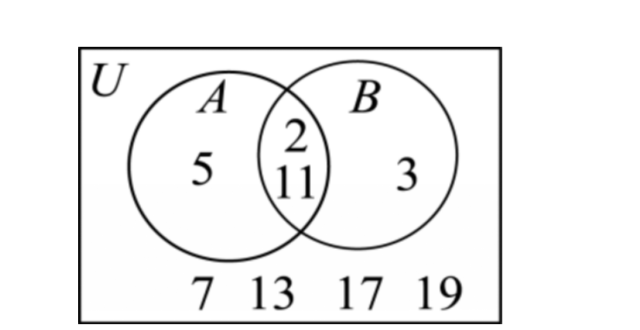
\includegraphics[width=0.24\textwidth]{figures/gao108_q6.png}
\end{center}

\solend
\fi

\item 若 $x\in A$，则 $\dfrac1x\in A$，就称 $A$ 自倒集合，集合 $M=\left\{-2,-1,0,\dfrac12,\dfrac13,1,2,3,4\right\}$ 的所有非空
子集中，自倒集合的个数为\blankline[4.4em].

\ifanswer
\solbegin
\step{由新定义，集合 $M$ 中的元素 1 和 $-1$ 倒数等于本身，2 和 $\dfrac12$，3 和 $\dfrac13$ 互为倒数,}
\step{故满足条件的自倒集合与集合 $\{-1,1,2,3\}$ 的非空子集的个数相同,}
\step{则其个数为 $2^4-1=15$.}
\solend
\fi

\item 设集合 $M=\{(x,y)\mid y=x^2+2bx+1\}$，$N=\{(x,y)\mid y=x+b\}(b\in\R)$，若
$M\cap N=\varnothing$，则实数 $b$ 的取值范围为\blankline[4.4em].

\ifanswer
\solbegin
\step{因为 $M\cap N=\varnothing$，所以
$\begin{cases}y=x^2+2bx+1\\y=x+b\end{cases}$
无解，则 $x^2+(2b-1)x+(1-b)=0$,}
\step{则 $\triangle=(2b-1)^2-4\times1\times(1-b)=4b^2-3<0$，解得 $-\dfrac{\sqrt3}2<b<\dfrac{\sqrt3}2$,}
\step{即实数 $b$ 的取值范围为 $\left(-\dfrac{\sqrt3}2,\dfrac{\sqrt3}2\right)$.}
\solend
\fi

\item 已知集合 $A=\left\{x\,\middle|\,\dfrac{x-a}{x^2-1}=1\right\}$ 有唯一元素，用列举法表示满足集合 $A$ 的条件的 $a$ 的取值集
合\blankline[4.4em].

\ifanswer
\solbegin
\step{$a=1$,$\dfrac{1}{x+1}=1$，一解；$a=-1$,$\dfrac{1}{x-1}=1$，一解；}
\step{$x-a=x^2-1$，一解时，$a=\dfrac54$,}
\step{综上，$a$ 的取值集合为 $\left\{-1,1,\dfrac54\right\}$.}
\solend
\fi

\item 已知集合 $M$ 的元素均为正整数，定义集合 $M$ 的“变项和”为：将 $M$ 中每个元素 $m$ 都乘
以 $(-1)^n$ 后再求和. 若集合 $A=\{n\mid1\leqslant n\leqslant2026,n\in\N\}$，则集合 $A$ 的所有非空子集的“变
项和”的总和为\blankline[4.4em].% $n$ 未加界定（据解析为元素序号），照录

\ifanswer
\solbegin
\step{$A=\{n\mid1\leqslant n\leqslant2026,n\in\N\}=\{1,2,\cdots,2026\}$,}
\step{1 在所有非空子集中共出现 $C_{2025}^{0}+C_{2025}^{1}+\cdots+C_{2025}^{2025}=2^{2025}$ 次,}
\step{同理 $2,3,\cdots,2026$ 都出现 $2^{2025}$ 次,}
\step{则集合 $A$ 的所有非空子集的“变项和”的总和}
\step{为 $2^{2025}\times[1\times(-1)^1+2\times(-1)^2+\cdots+2026\times(-1)^{2026}]$}
\step{$=2^{2025}\times(-1+2-3+4-\cdots-2025+2026)=1013\times2^{2025}$.}
\solend
\fi

\item 已知 $0<k<2$，定义 $[x]$ 为不超过 $x$ 的最大整数，区间 $[a,b]$（或 $(a,b)$，$[a,b)$，
$(a,b]$）的长度记为 $b-a$. 若关于 $x$ 的不等式 $k[x]>\lvert2[x]-6\rvert$ 的解集对应区间的长度为 $2$，
则 $k$ 的取值范围是\blankline[4.4em].

\ifanswer
\solbegin
\stepm{法一：}{由题意得 $\lvert2[x]-6\rvert=
\begin{cases}2[x]-6,x\geqslant3\\-2[x]+6,x<3\end{cases}$.}
\step{①当 $x\geqslant3$ 时，不等式 $k[x]>\lvert2[x]-6\rvert$ 可化为 $k[x]>2[x]-6$,}
\step{即 $(2-k)[x]<6$,}
\step{当 $0<k<2$ 时，解不等式 $(2-k)[x]<6$ 得 $[x]<\dfrac6{2-k}$.}
\step{②当 $x<3$ 时，不等式 $k[x]>\lvert2[x]-6\rvert$ 可化为 $k[x]>-2[x]+6$,}
\step{即 $(k+2)[x]>6$.}
\step{当 $0<k<2$ 时，解不等式 $(k+2)[x]>6$ 得 $[x]>\dfrac6{k+2}$.}
\step{综上所述，不等式 $k[x]>\lvert2[x]-6\rvert$ 的解集需满足 $\dfrac6{k+2}<[x]<\dfrac6{2-k}$,}
\step{由题意得在区间 $\left[\dfrac6{k+2},\dfrac6{2-k}\right]$ 内有两个整数,}
\step{由于 $\dfrac6{k+2}\in\left(\dfrac32,3\right)$，所以 $\dfrac6{2-k}\leqslant5$，得 $k\leqslant\dfrac45$.}
\step{因此 $k\in\left(0,\dfrac45\right]$，得 $\dfrac6{k+2}\in\left[\dfrac75,3\right)$，$\dfrac6{2-k}\in(3,5]$,}
\step{区间 $\left[\dfrac6{k+2},\dfrac6{2-k}\right]$ 内的两个整数是 3、4，所以 $4<\dfrac6{2-k}\leqslant5$，解得 $\dfrac12<k\leqslant\dfrac45$,}
\step{即 $k\in\left(\dfrac12,\dfrac45\right]$.}
\stepm{法二：}{令 $f(x)=kx$，$g(x)=\lvert2x-6\rvert$，画出 $g(x)$、$f(x)$ 的图象,}
\step{由于不等式 $k[x]>\lvert2[x]-6\rvert$ 的解集对应区间的长度为 2,}
\step{因此解集只可能为 $[3,5)$ 或 $[2,4)$.}
\step{当解集为 $[3,5)$ 时，如图（2），数形结合易得
$\begin{cases}f(2)\leqslant g(2)\\f(4)>g(4)\\f(5)\leqslant g(5)\end{cases}$,}
\step{即
$\begin{cases}2k\leqslant\lvert2\times2-6\rvert\\4k>\lvert2\times4-6\rvert\\5k\leqslant\lvert2\times5-6\rvert\end{cases}$，
解得
$\begin{cases}k\leqslant1\\k>\dfrac12\\k\leqslant\dfrac45\end{cases}$，
所以 $\dfrac12<k\leqslant\dfrac45$，满足 $0<k<2$,}
\step{当解集为 $[2,4)$ 时，如图（1），数形结合易得
$\begin{cases}f(2)>g(2)\\f(4)\leqslant g(4)\end{cases}$,}
\step{即
$\begin{cases}2k>\lvert2\times2-6\rvert\\4k\leqslant\lvert2\times4-6\rvert\end{cases}$，
无解.}

\begin{center}
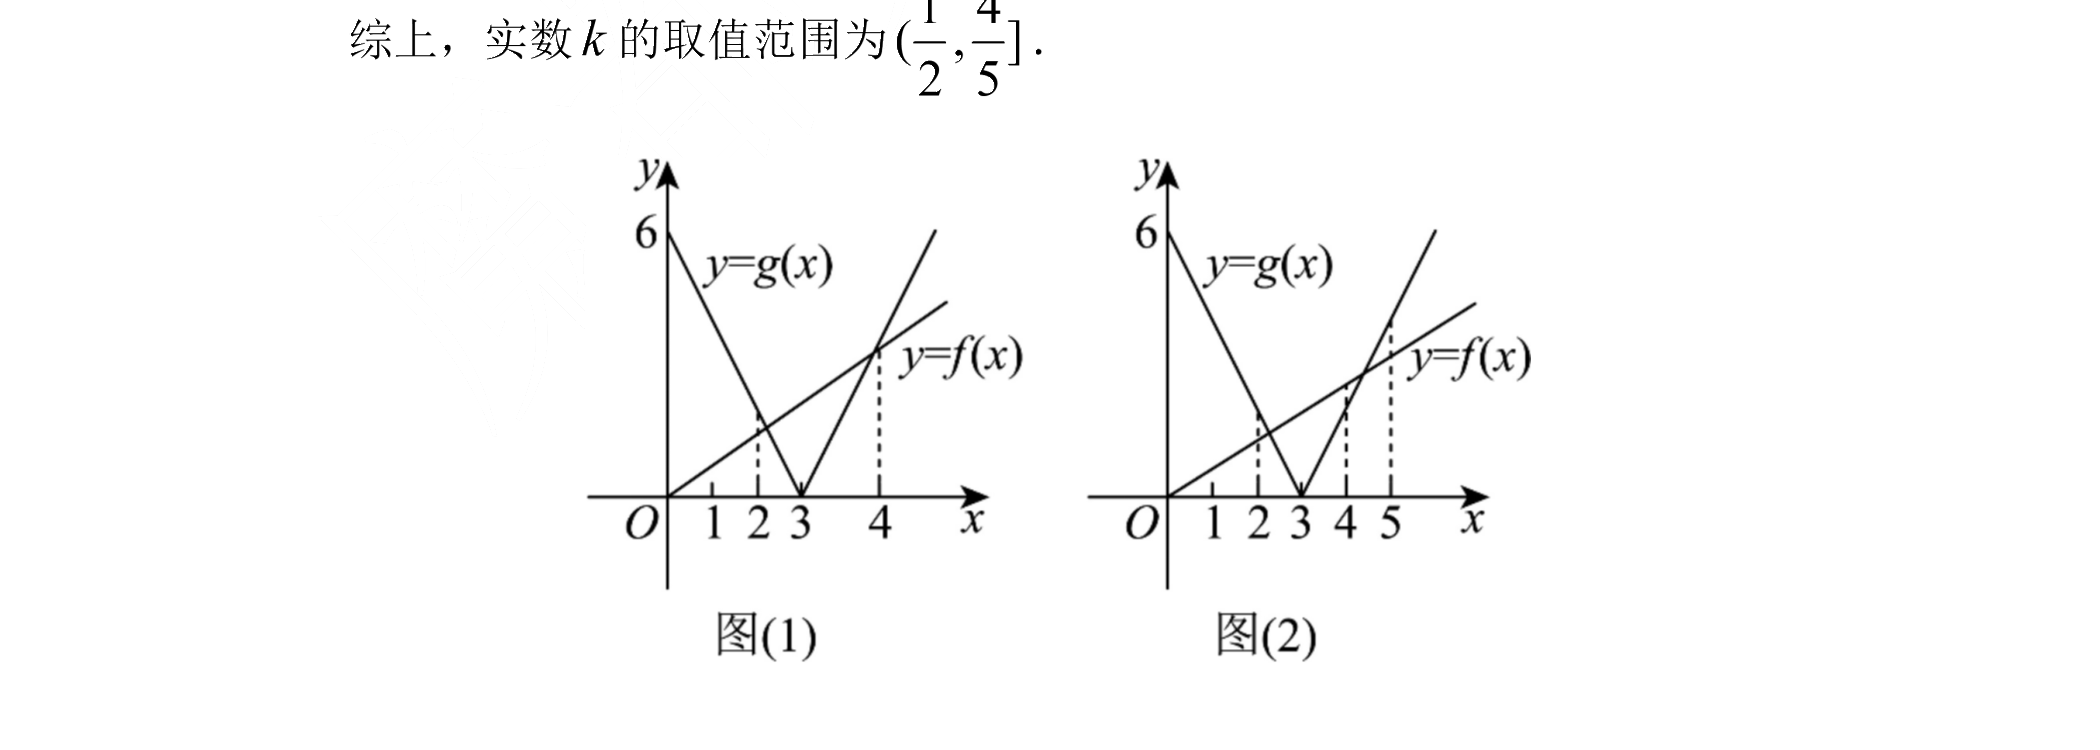
\includegraphics[width=0.72\textwidth]{figures/gao108_q11.png}
\end{center}

\step{综上，实数 $k$ 的取值范围为 $\left(\dfrac12,\dfrac45\right]$.}
\solend
\fi

\item 已知集合 $A=[1,a]\cup[a^3,a^4]$，集合 $B=\{x\mid x=x_1-x_2$，其中 $x_1$,$x_2\in A\}$. 若集合 $B$ 表
示的区间为一个闭区间，则实数 $a$ 的取值范围为\blankline[4.4em].

\ifanswer
\solbegin
\step{由题意得 $a^3>a>1$，则 $x_1-x_2$ 的最小值为 $1-a^4$，最大值为 $a^4-1$,}
\step{所以 $B=[1-a^4,a^4-1]$,}
\step{又因为 $a^4-a^3-(a-1)=a^3(a-1)-(a-1)=(a^3-1)(a-1)>0$,}
\step{所以 $a^4-a^3>a-1$，又集合 $B$ 表示的区间为一个闭区间,}
\step{则 $a^3-a\leqslant a^4-a^3$，化简得 $a^2-a-1\geqslant0$，又 $a>1$，解得 $a\geqslant\dfrac{1+\sqrt5}2$.}
\solend
\fi

\end{enumerate}

\bigsec{二、选择题}

\begin{enumerate}
\setcounter{enumi}{12}

\item 若 $a,b,c\in\R$，则下列不等式恒成立的是\mbox{（\quad）}% 原卷把答案“C”印在题干括号内、无【解析】

\keepwithprev
A. $\dfrac1a<\dfrac1b$\qquad B. $a^2<b^2$\qquad C. $\dfrac{a}{c^2+1}>\dfrac{b}{c^2+1}$\qquad D. $a\lvert c\rvert>b\lvert c\rvert$

\ifanswer
\ans{$C$}
\fi

\item 以下几个关系中正确的是\mbox{（\quad）}

\keepwithprev
A. $0\in\varnothing$\qquad\qquad\qquad B. $\varnothing\in\{x\mid x^2+1=0\}$

C. $\varnothing\subset\{0\}$\qquad\qquad\qquad D. $(A\cap B)\subset(A\cup B)$

\ifanswer
\solbegin
\step{$A$ 选项，$\varnothing$ 不包含任何元素，所以 $0\in\varnothing$ 错误，$A$ 错,}
\step{$B$ 选项，集合与集合之间关系不可以用 $\in$，$B$ 错,}
\step{$C$ 选项，空集是非空集合的真子集，所以 $\varnothing\subset\{0\}$ 正确，$C$ 对,}
\step{$D$ 选项，当 $A=B$ 时，$(A\cap B)=(A\cup B)$，$D$ 错,}
\step{故选 $C$.}
\solend
\fi

\item 设全集为 $U$，图中阴影部分所表示的集合是\mbox{（\quad）}% 原卷把答案“A”印在题干括号内、无【解析】

\keepwithprev
A. $B\cap\overline{A\cup C}$\qquad\qquad B. $(A\cup B)\cap(B\cup C)$

C. $(A\cup C)\cap\overline B$\qquad\qquad D. $(\overline A\cup\overline C)\cap B$

\ifanswer
\ans{$A$}
\fi

\item 对于 $k=0,1,2,\cdots$，定义集合 $A_k=\{20+k,26+2k\}$，并记 $S_k=A_0\cup A_1\cup\cdots\cup A_k$，则
使得集合 $S_n$ 中完全平方数的个数为奇数的最小正整数 $n$ 为\mbox{（\quad）}

\keepwithprev
A. $18$\qquad\qquad B. $19$\qquad\qquad C. $20$\qquad\qquad D. $21$

\ifanswer
\solbegin
\step{当 $k=0$ 时，$A_0=\{20,26\}$，对于 $k=0,1,2,\cdots$,}
\step{集合 $A_k$ 中最小的元素 $20>4^2$，若 $S_n$ 中完全平方数的个数为奇数，则 $n>4$,}
\step{（1）$20+k=5^2$ 时，$k=5$，$A_5=\{25,36\}$，此时 $S_5$ 中完全平方数为 $5^2$、$6^2$,}
\step{个数为 2;}
\step{$20+k=6^2$ 时，$k=16$，$A_{16}=\{36,58\}$，此时 $S_{16}$ 中完全平方数为 $5^2$、$6^2$,}
\step{个数为 2;}
\step{$20+k=7^2$ 时，$k=29$，$A_{29}=\{49,84\}$,}
\step{此时 $S_{29}$ 中完全平方数为 $5^2$、$6^2$、$7^2$、$8^2$，个数为 4;}
\step{$20+k=8^2$ 时，$k=44$，$A_{44}=\{64,114\}$,}
\step{此时 $S_{44}$ 中完全平方数为 $5^2$、$6^2$、$7^2$、$8^2$、$10^2$，个数为 5;}
\step{（2）因为 $k=0,1,2,\cdots,26+2k$ 一定为偶数,}
\step{所以 $26+2k=6^2$ 时，$k=5$，由上述分析得 $S_5$ 中完全平方数个数为 2;}
\step{$26+2k=8^2$ 时，$k=19$，$A_{19}=\{39,64\}$,}
\step{此时 $S_{19}$ 中完全平方数为 $5^2$、$6^2$、$8^2$，个数为 3.}
\step{综上，使集合 $S_n$ 中完全平方数的个数为奇数的最小正整数 $n=19$. 故选 $B$.}
\solend
\fi

\end{enumerate}

\bigsec{三、解答题}

\begin{enumerate}
\setcounter{enumi}{16}

\item 设全集 $U=\R$，集合 $A=\left\{x\,\middle|\,\dfrac{x-2}{x+2}\leqslant0\right\}$，$B=\{x\mid a\leqslant x<2a+1,a\in\R\}$，
$C=\{x\mid\lvert2x-1\rvert<5\}$.

（1）求集合 $A$、$\overline A\cup C$；

（2）若 $B\subseteq A$，求实数 $a$ 的取值范围.

\ifanswer
\solbegin
\ansspace*
\step{（1）不等式 $\dfrac{x-2}{x+2}\leqslant0$，等价于
$\begin{cases}(x-2)(x+2)\leqslant0\\x+2\neq0\end{cases}$，
解得 $\{x\mid-2<x\leqslant2\}$,}
\step{所以 $A=\{x\mid-2<x\leqslant2\}$，则 $\overline A=\{x\mid x\leqslant-2$ 或 $x>2\}$,}
\step{因为 $C=\{x\mid\lvert2x-1\rvert<5\}=\{x\mid-2<x<3\}$，所以 $\overline A\cup C=\R$；}
\step{（2）因为 $B\subseteq A$,}
\step{若 $B=\varnothing$，则 $a\geqslant2a+1$，解得 $a\leqslant-1$,}
\step{若 $B\neq\varnothing$，则
$\begin{cases}a<2a+1\\a>-2\\2a+1\leqslant2\end{cases}$，
解得 $-1<a\leqslant\dfrac12$,}
\step{综上所述，实数 $a$ 的取值范围为 $\left\{a\,\middle|\,a\leqslant\dfrac12\right\}$.}
\solend
\fi

\item 设 $a$、$b$、$c$、$d$ 是四个正数.

（1）已知 $a>b$，比较 $\dfrac{2a+b}{a+2b}$ 与 $\dfrac ab$ 的值的大小；

（2）若 $(1+a)(1+b)(1+c)(1+d)<16$，求证：$a$、$b$、$c$、$d$ 中至少有一个小于 1.

\ifanswer
\solbegin
\step{（1）$\dfrac{2a+b}{a+2b}-\dfrac ab=\dfrac{b^2-a^2}{b(a+2b)}<0$，所以 $\dfrac{2a+b}{a+2b}<\dfrac ab$.}
\step{（2）假设 $a$、$b$、$c$、$d$ 都不小于 1，即 $a$、$b$、$c$、$d$ 均大于等于 1,}
\step{即 $a\geqslant1$，$b\geqslant1$，$c\geqslant1$，$d\geqslant1$,}
\step{由均值不等式得 $1+a\geqslant2\sqrt a$,$1+b\geqslant2\sqrt b$,$1+c\geqslant2\sqrt c$,$1+d\geqslant2\sqrt d$,}
\step{故 $(1+a)(1+b)(1+c)(1+d)\geqslant16\sqrt{abcd}\geqslant16$,}
\step{当且仅当 $a=b=c=d=1$ 时取等号,}
\step{这与 $(1+a)(1+b)(1+c)(1+d)<16$ 矛盾，故假设不成立，原命题成立.}
\solend
\fi

\item 已知 $m\in\R$，一个二次项系数为 1 的一元二次方程的两个不等实根分别为 $x_1$ 和 $x_2$，且
满足
$\begin{cases}x_1^2+x_2^2=2m^2-4\\x_1+x_2=m\end{cases}$.

（1）直接写出该一元二次方程；

（2）若 $(3x_1-x_2)(3x_2-x_1)\geqslant-1$，求 $m$ 的取值范围；

（3）若方程的两根 $x_1$ 和 $x_2$ 都大于 $-1$，求 $m$ 的取值范围.

\ifanswer
\solbegin
\step{（1）设这个一元二次方程为 $x^2+bx+c=0$,}
\step{由
$\begin{cases}x_1^2+x_2^2=2m^2-4\\x_1+x_2=m\end{cases}$,}
\step{得 $(x_1+x_2)^2=x_1^2+x_2^2+2x_1x_2=2m^2-4+2x_1x_2=m^2$，即 $x_1x_2=\dfrac{4-m^2}2$,}
\step{由韦达定理得 $x_1+x_2=-b=m$，即 $x_1x_2=c=\dfrac{4-m^2}2$,}
\step{所以一元二次方程为 $x^2-mx+\dfrac{4-m^2}2=0$.}
\step{（2）$(3x_1-x_2)(3x_2-x_1)=9x_1x_2-3x_1^2-3x_2^2+x_1x_2=10x_1x_2-3(x_1^2+x_2^2)\geqslant-1$,}
\step{结合已知及（1）得 $x_1^2+x_2^2=2m^2-4$,$x_1x_2=\dfrac{4-m^2}2$,}
\step{代入得 $10\times\dfrac{4-m^2}2-3(2m^2-4)=-11m^2+32\geqslant-1\Rightarrow m^2\leqslant3$}
\step{$\Rightarrow-\sqrt3\leqslant m\leqslant\sqrt3$,}
\step{又 $\Delta=m^2-4\times\dfrac{4-m^2}2=3m^2-8>0\Rightarrow m<-\dfrac{2\sqrt6}3$ 或 $m>\dfrac{2\sqrt6}3$,}
\step{所以 $m\in\left[-\sqrt3,-\dfrac{2\sqrt6}3\right)\cup\left(\dfrac{2\sqrt6}3,\sqrt3\right]$.}
\step{（3）若方程的两根 $x_1$ 和 $x_2$ 都大于 $-1$，则
$\begin{cases}\Delta>0\\x_1+x_2>-2\\(x_1+1)(x_2+1)>0\end{cases}$,}
\step{所以
$\begin{cases}\Delta=3m^2-8>0\\m>-2\\[2pt]\dfrac{4-m^2}2+m+1>0\end{cases}$，
解得 $m\in\left(1-\sqrt7,-\dfrac{2\sqrt6}3\right)\cup\left(\dfrac{2\sqrt6}3,1+\sqrt7\right)$.}
\solend
\fi

\item 已知不等式 $2\leqslant ax^2+bx+c\leqslant3$ 的解集为 $\{x\mid2\leqslant x\leqslant3\}$.

（1）若 $a>0$，求 $6b+5c$ 的值；

（2）若 $a>0$，且不等式 $ax^2+(b-3)x-c\leqslant0$ 有且仅有 9 个整数解，求 $a$ 的取值范围；

（3）若 $a<0$，对任意的 $x<0$，不等式 $(ax-4)(x^2+b+c+1)\geqslant0$ 恒成立，求 $a^2-b+c$
的取值集合.

\ifanswer
\solbegin
\ansspace*
\step{（1）$a>0$,}
\step{结合二次函数图象得不等式 $ax^2+bx+c\leqslant3$ 的解集为 $\{x\mid2\leqslant x\leqslant3\}$,}
\step{且不等式 $ax^2+bx+c\geqslant2$ 的解集为 $R$,}
\step{所以方程 $ax^2+bx+c-3=0$ 的两根分别为 2 和 3,}
\step{则
$\begin{cases}2+3=-\dfrac ba\\[2pt]2\times3=\dfrac{c-3}a\end{cases}$，
得 $b=-5a$，$c=6a+3$,}
\step{所以 $6b+5c=6\times(-5a)+5(6a+3)=15$.}
\step{（2）若 $a>0$，且不等式 $ax^2+(b-3)x-c\leqslant0$ 有且仅有 9 个整数解,}
\step{由（1）得 $b=-5a$，$c=6a+3$,}
\step{不等式 $ax^2+bx+c\geqslant2$ 可化为 $ax^2-5ax+6a+1\geqslant0$.}
\step{由（1）得不等式 $ax^2+bx+c\geqslant2$ 的解集为 $R$,}
\step{所以 $ax^2-5ax+6a+1\geqslant0$ 恒成立,}
\step{所以
$\begin{cases}a>0\\\Delta=25a^2-4a(6a+1)\leqslant0\end{cases}$，
即
$\begin{cases}a>0\\a^2-4a=a(a-4)\leqslant0\end{cases}$，}
\step{解得 $0<a\leqslant4$.}
\step{不等式 $ax^2+(b-3)x-c\leqslant0$ 等价于 $ax^2-(5a+3)x-(6a+3)\leqslant0$,}
\step{所以 $[ax-(6a+3)](x+1)\leqslant0$，得 $-1\leqslant x\leqslant6+\dfrac3a$,}
\step{所以 $7\leqslant6+\dfrac3a<8$，解得 $\dfrac32<a\leqslant3$.}
\step{综上，$a$ 的取值范围为 $\left(\dfrac32,3\right]$.}
\step{（3）因为 $a<0$,}
\step{同（1）分析，不等式 $ax^2+bx+c\geqslant2$ 的解集为 $\{x\mid2\leqslant x\leqslant3\}$,}
\step{$ax^2+bx+c\leqslant3$ 的解集为 $R$,}
\step{所以方程 $ax^2+bx+c-2=0$ 的两根分别为 2 和 3,}
\step{则
$\begin{cases}2+3=-\dfrac ba\\[2pt]2\times3=\dfrac{c-2}a\end{cases}$，
得 $b=-5a$，$c=6a+2$.}
\step{所以不等式 $ax^2+bx+c=ax^2-5ax+6a+2\leqslant3$ 的解集为 $R$,}
\step{则 $ax^2-5ax+6a-1\leqslant0$ 恒成立,}
\step{所以
$\begin{cases}a<0\\\Delta=25a^2-4a(6a-1)\leqslant0\end{cases}$，
即
$\begin{cases}a<0\\a^2+4a=a(a+4)\leqslant0\end{cases}$，}
\step{解得 $-4\leqslant a<0$.}
\step{所以对任意的 $x<0$，不等式 $(ax-4)(x^2+b+c+1)\geqslant0$ 恒成立}
\step{转化为对任意的 $x<0$，不等式 $(ax-4)(x^2+a+3)\geqslant0$ 恒成立.}
\step{方程 $(ax-4)(x^2+a+3)=0$ 的两个根为 $x=\dfrac4a<0$,}
\step{$x=\pm\sqrt{-a-3}$（$a<-3$ 时成立）,}
\step{因而仅当 $ax-4=0$ 与 $x^2+a+3=0$ 的负根重合时满足条件,}
\step{解得唯一解为 $a=-4$，所以 $a^2-b+c=a^2+11a+2=-26$,}
\step{所以 $a^2-b+c$ 的取值集合为 $\{-26\}$.}
\solend
\fi

\item 已知集合 $A=\{1,2,3,4,5,6,7,8\}$，$M=\{(x,y)\mid x\in A,y\in A\}$，从 $M$ 中选取 $n$ 个不同的
元素组成一个序列：$(x_1,y_1)$,$(x_2,y_2),\cdots,(x_n,y_n)$，其中 $(x_i,y_i)$ 称为该序列的第 $i$ 项
（$i=1,2,\cdots,n$），若该序列的相邻项 $(x_i,y_i)$,$(x_{i+1},y_{i+1})$ 满足：
\[\begin{cases}\lvert x_{i+1}-x_i\rvert=3\\\lvert y_{i+1}-y_i\rvert=4\end{cases}
\quad\text{或}\quad
\begin{cases}\lvert x_{i+1}-x_i\rvert=4\\\lvert y_{i+1}-y_i\rvert=3\end{cases}\]
（$i=1,2,\cdots,n-1$），则称该序列为“$\Delta-$序列”.

（1）若一个 $\Delta-$序列的第一项为 $(4,4)$，请直接写出它所有可能的第二项；

（2）定义集合 $A=\{1,2,3,4,5,6,7,8\}$ 的两个子集：外侧集 $S=\{1,2,7,8\}$，内侧集
$T=\{3,4,5,6\}$. 证明：若 $\Delta-$序列中某一项的坐标在区域 $S\times S$ 内（即横、纵坐标均属于
$S$），则它的下一项坐标必定在区域 $T\times T$ 内；

（3）证明：不存在一个恰好有 5 项的 $\Delta-$序列，使其第一项为 $(1,8)$，且第五项为
$(8,1)$.

\ifanswer
\solbegin
\ansspace*
\step{（1）由题意，第一项为 $(x_1,y_1)=(4,4)$,}
\step{对于第二项 $(x_2,y_2)$，其坐标必须在 1~8 之间.}
\step{若 $\lvert x_2-4\rvert=3$,$\lvert y_2-4\rvert=4$，则 $x_2\in\{1,7\}$,}
\step{且 $y_2\in\{8\}$（因为 $4-4=0$ 不在集合 $A$ 中）. 此时可能的点为 $(1,8)$,$(7,8)$.}
\step{若 $\lvert x_2-4\rvert=4$,$\lvert y_2-4\rvert=3$，则 $x_2\in\{8\}$，且 $y_2\in\{1,7\}$.}
\step{此时可能的点为 $(8,1)$,$(8,7)$.}
\step{所以它所有可能的第二项为 $(1,8)$,$(7,8)$,$(8,1)$,$(8,7)$.}
\step{（2）已知某一项 $(x_t,y_t)\in S\times S$，即 $x_t\in\{1,2,7,8\}$ 且 $y_t\in\{1,2,7,8\}$.}
\step{由规则得下一步坐标的变化量为 3 和 4，设 $a\in S$ 变化 3 或 4 后的结果 $a'$:}
\step{当 $a=1$ 时，$1+3=4\in T$,$1+4=5\in T$；}
\step{当 $a=2$ 时，$2+3=5\in T$,$2+4=6\in T$；}
\step{当 $a=7$ 时，$7-3=4\in T$,$7-4=3\in T$；}
\step{当 $a=8$ 时，$8-3=5\in T$,$8-4=4\in T$.}
\step{（注：由于超出 1~8 范围的越界坐标不符合.）}
\step{由此可见，无论 $a$ 是 $S$ 中的哪一个数，加上或减去 3 或 4 之后,}
\step{得到的新坐标必属于集合 $T$.}
\step{因为 $\Delta-$序列每走一步，横坐标和纵坐标必定同时发生 3 和 4 的变化,}
\step{所以新的横坐标 $x_{i+1}$ 必属于 $T$，新的纵坐标 $y_{i+1}$ 也必属于 $T$,}
\step{即下一项 $(x_{i+1},y_{i+1})$ 必定在区域 $T\times T$ 内. ………10 分原命题得证.% 得分行混入证明，照录
}
\step{（3）假设存在这样一个包含 5 项的 $\Delta-$序列:}
\step{$(x_1,y_1)$,$(x_2,y_2)$,$(x_3,y_3)$,$(x_4,y_4)$,$(x_5,y_5)$.}
\step{已知第一项为 $(1,8)$，第五项为 $(8,1)$. 第 2 项必须是第 1 项 $(1,8)$ 的相邻点.}
\step{我们来找 $(1,8)$ 的相邻点：第 2 项只能是 $(4,4)$ 或 $(5,5)$,}
\step{第 4 项必须是第 5 项 $(8,1)$ 的相邻点（因为跳跃是双向可逆的）.}
\step{同理可算得，$(8,1)$ 的相邻点也只有两个：$(4,4)$ 和 $(5,5)$,}
\step{题目题干中明确规定，$\Delta-$序列由 $n$ 个不同的有序数对构成.% “题目题干”措辞重复，照录
}
\step{所以，第 2 项和第 4 项不能是同一个点. 这就意味着:}
\step{如果第 2 项是 $(4,4)$，第 4 项就必须是 $(5,5)$；反之亦然.}
\step{则第 3 项必须是 $(4,4)$ 和 $(5,5)$ 的公共相邻点.}
\step{$(4,4)$ 的相邻点集合为：$\{(1,8),(7,8),(8,1),(8,7)\}$,}
\step{$(5,5)$ 的相邻点集合为：$\{(2,1),(8,1),(1,2),(1,8)\}$,}
\step{所以，第 3 项只能填 $(1,8)$ 或者 $(8,1)$.}
\step{这与“序列由不同的有序数对构成”这一条件产生矛盾！}
\step{所以，不存在一个恰好有 5 项的 $\Delta-$序列,}
\step{使其第一项为 $(1,8)$，且第五项为 $(8,1)$.}
\solend
\fi

\end{enumerate}

\end{document}
"
% 紧凑版：xelatex "\def\iscompact{1}% 高一108_五校联考_10月月考.tex
%   —— 高一上数学“2026-2027 年五校联考高一上 10 月月考”（试卷版/答案版）
% 试卷版：xelatex 高一108_五校联考_10月月考.tex
% 答案版：xelatex "\def\isanswer{1}\input{高一108_五校联考_10月月考.tex}"
% 紧凑版：xelatex "\def\iscompact{1}\input{高一108_五校联考_10月月考.tex}"
%
% 原始材料：微信公众号“魔都数学加油站”文章，作者破晓，2026-11-03 17:19 发布；
% 连载“27学年高一108”，原文标题“27学年高一108——2026-2027年上海市五校联考高一上10月月考”；
% 原文链接：https://mp.weixin.qq.com/s/3nkP789Qar93NGMZXFFCSw。
% 正文为 14 张 PNG 页（第 2、3、6—13 页 4762×6735，第 1、4、5、14 页 2560×3620），
% 题目下印有【解析】，为讲评版。
% 题目、解析均据原图转录；卷面水印及公众号页脚未录入。
% 第 6 题解析的文氏图与第 11 题法二解析的两幅图象（图(1)、图(2)）裁自原图、去粉色水印
% 转灰度（gao108_q6.png、gao108_q11.png），第 6 题图属解析（仅答案版）、
% 第 11 题图属解析（仅答案版）。
%
% 卷首标题：原卷印作“2026-2027 年五校联考高一上 10 月月考”，标题下另印一行参与学校
% 名单“闵行中学、嘉定一中、松江一中、金山中学、嘉一实高”（全稿第 5 份原卷自印副标题，
% 按 14／24／49／50 成例照录，并登记进计数核对.py 的 SELFSUB）。
%
% 与原卷的排版差异：
%   ① 原文从第 3 题起，填空题编号为 3—12、选择题为 13—16、解答题为 17—21，本稿保留原题号；
%   ② 原卷每题下直接印【解析】，本稿按全稿惯例将解析置于答案版；第 4 题只印【答案】，
%      第 13、15 两题把答案印在题干括号内且无【解析】，均另提 \ans{}；
%   ③ 原卷副标题照录（见上）；
%   ④ 原卷填空横线按全稿惯例排为 \blankline[4.4em]；解答题按惯例加 \ansspace；选择题括号排
%      \mbox{（\quad）}、选项段前按惯例加 \keepwithprev；
%   ⑤ 原卷数集排斜体 $R$／$N$，按全稿惯例改 \R、\N。
%
% 原卷红色强调照录为黑体：第 11 题解析的“法一：”“法二：”原卷排红色，按 53 成例排
% \stepm{法一：}／\stepm{法二：}（加粗着色）。
%
% 原卷存疑：第 10 题题干“变项和”定义中“将 $M$ 中每个元素 $m$ 都乘以 $(-1)^n$ 后再求和”
% 的 $n$ 未加界定（据解析应为该元素在 $\{1,2,\cdots,2026\}$ 中的序号），照录。
% 第 21 题 (2) 解析末行“即下一项 $(x_{i+1},y_{i+1})$ 必定在区域 $T\times T$ 内. ………10 分
% 原命题得证.”，原卷把得分点行混入证明（“原命题”按上下文为“原命题的逆否”），照录。
% 第 21 题 (3) 解析“题目题干中明确规定”，“题目题干”措辞重复，照录。
%
% 行数核对：逐题数 \step/\stepm 条数，合计 164 条（Q3：3；Q4：0；Q5：2；Q6：1；Q7：3；
% Q8：3；Q9：3；Q10：6；Q11：21；Q12：5；Q13：0；Q14：5；Q15：0；Q16：15；Q17：7；
% Q18：7；Q19：13；Q20：34；Q21：36），与原卷印刷行逐题相等。第 4 题只印【答案】、
% 第 13、15 题括号内印答案，均提 \ans{}，不计入 \step 账。
%
\documentclass[a4paper,11pt]{article}
\usepackage{common}

\begin{document}

\examtitlest[3]{2026--2027 年五校联考高一上 10 月月考}{闵行中学、嘉定一中、松江一中、金山中学、嘉一实高}

\bigsec{一、填空题}

\begin{enumerate}
\setcounter{enumi}{2}

\item 已知等式 $2x^2+3x+5=2ax^2+a(3x+1)+c$ 恒成立，则实数 $a+c$ 的值为\blankline[4.4em].

\ifanswer
\solbegin
\step{因为 $2x^2+3x+5=2ax^2+a(3x+1)+c$ 恒成立,}
\step{即 $2x^2+3x+5=2ax^2+3ax+(a+c)$ 恒成立，所以
$\begin{cases}2=2a\\3=3a\\5=a+c\end{cases}$,}
\step{所以 $a+c=5$.}
\solend
\fi

\item 不等式 $\dfrac1x<\dfrac12$ 的解集是\blankline[4.4em].

\ifanswer
\ans{$(-\infty,0)\cup(2,+\infty)$}
\fi

\item 已知 $a$、$b$ 都是实数，则“$a^2=b^2$”是“$a^2+b^2=2ab$”的\blankline[4.4em]条件.

\ifanswer
\solbegin
\step{$a^2=b^2$ 等价于 $a=\pm b$；$a^2+b^2=2ab$ 等价于 $(a-b)^2=0$ 等价于 $a=b$,}
\step{故“$a^2=b^2$”是“$a^2+b^2=2ab$”的必要不充分条件.}
\solend
\fi

\item 已知全集 $U=\{x\mid x$ 为不大于 20 的素数$\}$，$A\cap\overline B=\{5\}$，$\overline A\cap B=\{3\}$，
$\overline{A\cup B}=\{7,13,17,19\}$，则 $A=$\blankline[4.4em].

\ifanswer
\solbegin
\step{如图所示，$A=\{2,5,11\}$.}

\begin{center}
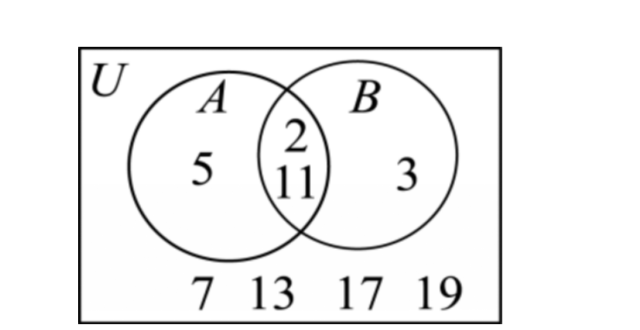
\includegraphics[width=0.24\textwidth]{figures/gao108_q6.png}
\end{center}

\solend
\fi

\item 若 $x\in A$，则 $\dfrac1x\in A$，就称 $A$ 自倒集合，集合 $M=\left\{-2,-1,0,\dfrac12,\dfrac13,1,2,3,4\right\}$ 的所有非空
子集中，自倒集合的个数为\blankline[4.4em].

\ifanswer
\solbegin
\step{由新定义，集合 $M$ 中的元素 1 和 $-1$ 倒数等于本身，2 和 $\dfrac12$，3 和 $\dfrac13$ 互为倒数,}
\step{故满足条件的自倒集合与集合 $\{-1,1,2,3\}$ 的非空子集的个数相同,}
\step{则其个数为 $2^4-1=15$.}
\solend
\fi

\item 设集合 $M=\{(x,y)\mid y=x^2+2bx+1\}$，$N=\{(x,y)\mid y=x+b\}(b\in\R)$，若
$M\cap N=\varnothing$，则实数 $b$ 的取值范围为\blankline[4.4em].

\ifanswer
\solbegin
\step{因为 $M\cap N=\varnothing$，所以
$\begin{cases}y=x^2+2bx+1\\y=x+b\end{cases}$
无解，则 $x^2+(2b-1)x+(1-b)=0$,}
\step{则 $\triangle=(2b-1)^2-4\times1\times(1-b)=4b^2-3<0$，解得 $-\dfrac{\sqrt3}2<b<\dfrac{\sqrt3}2$,}
\step{即实数 $b$ 的取值范围为 $\left(-\dfrac{\sqrt3}2,\dfrac{\sqrt3}2\right)$.}
\solend
\fi

\item 已知集合 $A=\left\{x\,\middle|\,\dfrac{x-a}{x^2-1}=1\right\}$ 有唯一元素，用列举法表示满足集合 $A$ 的条件的 $a$ 的取值集
合\blankline[4.4em].

\ifanswer
\solbegin
\step{$a=1$,$\dfrac{1}{x+1}=1$，一解；$a=-1$,$\dfrac{1}{x-1}=1$，一解；}
\step{$x-a=x^2-1$，一解时，$a=\dfrac54$,}
\step{综上，$a$ 的取值集合为 $\left\{-1,1,\dfrac54\right\}$.}
\solend
\fi

\item 已知集合 $M$ 的元素均为正整数，定义集合 $M$ 的“变项和”为：将 $M$ 中每个元素 $m$ 都乘
以 $(-1)^n$ 后再求和. 若集合 $A=\{n\mid1\leqslant n\leqslant2026,n\in\N\}$，则集合 $A$ 的所有非空子集的“变
项和”的总和为\blankline[4.4em].% $n$ 未加界定（据解析为元素序号），照录

\ifanswer
\solbegin
\step{$A=\{n\mid1\leqslant n\leqslant2026,n\in\N\}=\{1,2,\cdots,2026\}$,}
\step{1 在所有非空子集中共出现 $C_{2025}^{0}+C_{2025}^{1}+\cdots+C_{2025}^{2025}=2^{2025}$ 次,}
\step{同理 $2,3,\cdots,2026$ 都出现 $2^{2025}$ 次,}
\step{则集合 $A$ 的所有非空子集的“变项和”的总和}
\step{为 $2^{2025}\times[1\times(-1)^1+2\times(-1)^2+\cdots+2026\times(-1)^{2026}]$}
\step{$=2^{2025}\times(-1+2-3+4-\cdots-2025+2026)=1013\times2^{2025}$.}
\solend
\fi

\item 已知 $0<k<2$，定义 $[x]$ 为不超过 $x$ 的最大整数，区间 $[a,b]$（或 $(a,b)$，$[a,b)$，
$(a,b]$）的长度记为 $b-a$. 若关于 $x$ 的不等式 $k[x]>\lvert2[x]-6\rvert$ 的解集对应区间的长度为 $2$，
则 $k$ 的取值范围是\blankline[4.4em].

\ifanswer
\solbegin
\stepm{法一：}{由题意得 $\lvert2[x]-6\rvert=
\begin{cases}2[x]-6,x\geqslant3\\-2[x]+6,x<3\end{cases}$.}
\step{①当 $x\geqslant3$ 时，不等式 $k[x]>\lvert2[x]-6\rvert$ 可化为 $k[x]>2[x]-6$,}
\step{即 $(2-k)[x]<6$,}
\step{当 $0<k<2$ 时，解不等式 $(2-k)[x]<6$ 得 $[x]<\dfrac6{2-k}$.}
\step{②当 $x<3$ 时，不等式 $k[x]>\lvert2[x]-6\rvert$ 可化为 $k[x]>-2[x]+6$,}
\step{即 $(k+2)[x]>6$.}
\step{当 $0<k<2$ 时，解不等式 $(k+2)[x]>6$ 得 $[x]>\dfrac6{k+2}$.}
\step{综上所述，不等式 $k[x]>\lvert2[x]-6\rvert$ 的解集需满足 $\dfrac6{k+2}<[x]<\dfrac6{2-k}$,}
\step{由题意得在区间 $\left[\dfrac6{k+2},\dfrac6{2-k}\right]$ 内有两个整数,}
\step{由于 $\dfrac6{k+2}\in\left(\dfrac32,3\right)$，所以 $\dfrac6{2-k}\leqslant5$，得 $k\leqslant\dfrac45$.}
\step{因此 $k\in\left(0,\dfrac45\right]$，得 $\dfrac6{k+2}\in\left[\dfrac75,3\right)$，$\dfrac6{2-k}\in(3,5]$,}
\step{区间 $\left[\dfrac6{k+2},\dfrac6{2-k}\right]$ 内的两个整数是 3、4，所以 $4<\dfrac6{2-k}\leqslant5$，解得 $\dfrac12<k\leqslant\dfrac45$,}
\step{即 $k\in\left(\dfrac12,\dfrac45\right]$.}
\stepm{法二：}{令 $f(x)=kx$，$g(x)=\lvert2x-6\rvert$，画出 $g(x)$、$f(x)$ 的图象,}
\step{由于不等式 $k[x]>\lvert2[x]-6\rvert$ 的解集对应区间的长度为 2,}
\step{因此解集只可能为 $[3,5)$ 或 $[2,4)$.}
\step{当解集为 $[3,5)$ 时，如图（2），数形结合易得
$\begin{cases}f(2)\leqslant g(2)\\f(4)>g(4)\\f(5)\leqslant g(5)\end{cases}$,}
\step{即
$\begin{cases}2k\leqslant\lvert2\times2-6\rvert\\4k>\lvert2\times4-6\rvert\\5k\leqslant\lvert2\times5-6\rvert\end{cases}$，
解得
$\begin{cases}k\leqslant1\\k>\dfrac12\\k\leqslant\dfrac45\end{cases}$，
所以 $\dfrac12<k\leqslant\dfrac45$，满足 $0<k<2$,}
\step{当解集为 $[2,4)$ 时，如图（1），数形结合易得
$\begin{cases}f(2)>g(2)\\f(4)\leqslant g(4)\end{cases}$,}
\step{即
$\begin{cases}2k>\lvert2\times2-6\rvert\\4k\leqslant\lvert2\times4-6\rvert\end{cases}$，
无解.}

\begin{center}
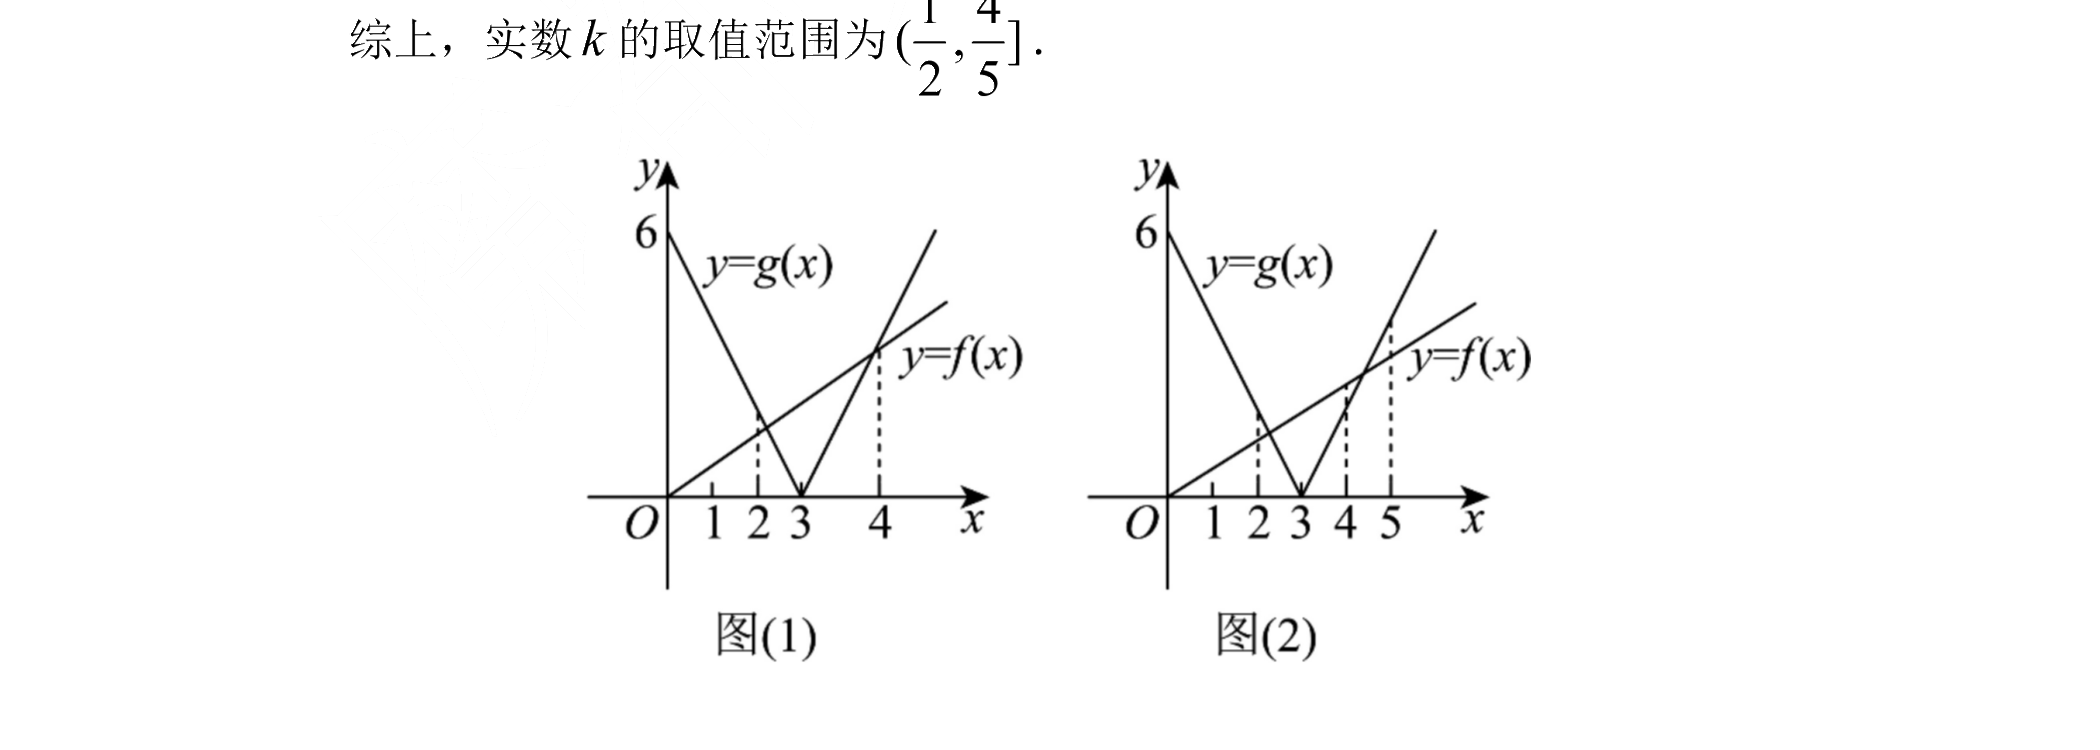
\includegraphics[width=0.72\textwidth]{figures/gao108_q11.png}
\end{center}

\step{综上，实数 $k$ 的取值范围为 $\left(\dfrac12,\dfrac45\right]$.}
\solend
\fi

\item 已知集合 $A=[1,a]\cup[a^3,a^4]$，集合 $B=\{x\mid x=x_1-x_2$，其中 $x_1$,$x_2\in A\}$. 若集合 $B$ 表
示的区间为一个闭区间，则实数 $a$ 的取值范围为\blankline[4.4em].

\ifanswer
\solbegin
\step{由题意得 $a^3>a>1$，则 $x_1-x_2$ 的最小值为 $1-a^4$，最大值为 $a^4-1$,}
\step{所以 $B=[1-a^4,a^4-1]$,}
\step{又因为 $a^4-a^3-(a-1)=a^3(a-1)-(a-1)=(a^3-1)(a-1)>0$,}
\step{所以 $a^4-a^3>a-1$，又集合 $B$ 表示的区间为一个闭区间,}
\step{则 $a^3-a\leqslant a^4-a^3$，化简得 $a^2-a-1\geqslant0$，又 $a>1$，解得 $a\geqslant\dfrac{1+\sqrt5}2$.}
\solend
\fi

\end{enumerate}

\bigsec{二、选择题}

\begin{enumerate}
\setcounter{enumi}{12}

\item 若 $a,b,c\in\R$，则下列不等式恒成立的是\mbox{（\quad）}% 原卷把答案“C”印在题干括号内、无【解析】

\keepwithprev
A. $\dfrac1a<\dfrac1b$\qquad B. $a^2<b^2$\qquad C. $\dfrac{a}{c^2+1}>\dfrac{b}{c^2+1}$\qquad D. $a\lvert c\rvert>b\lvert c\rvert$

\ifanswer
\ans{$C$}
\fi

\item 以下几个关系中正确的是\mbox{（\quad）}

\keepwithprev
A. $0\in\varnothing$\qquad\qquad\qquad B. $\varnothing\in\{x\mid x^2+1=0\}$

C. $\varnothing\subset\{0\}$\qquad\qquad\qquad D. $(A\cap B)\subset(A\cup B)$

\ifanswer
\solbegin
\step{$A$ 选项，$\varnothing$ 不包含任何元素，所以 $0\in\varnothing$ 错误，$A$ 错,}
\step{$B$ 选项，集合与集合之间关系不可以用 $\in$，$B$ 错,}
\step{$C$ 选项，空集是非空集合的真子集，所以 $\varnothing\subset\{0\}$ 正确，$C$ 对,}
\step{$D$ 选项，当 $A=B$ 时，$(A\cap B)=(A\cup B)$，$D$ 错,}
\step{故选 $C$.}
\solend
\fi

\item 设全集为 $U$，图中阴影部分所表示的集合是\mbox{（\quad）}% 原卷把答案“A”印在题干括号内、无【解析】

\keepwithprev
A. $B\cap\overline{A\cup C}$\qquad\qquad B. $(A\cup B)\cap(B\cup C)$

C. $(A\cup C)\cap\overline B$\qquad\qquad D. $(\overline A\cup\overline C)\cap B$

\ifanswer
\ans{$A$}
\fi

\item 对于 $k=0,1,2,\cdots$，定义集合 $A_k=\{20+k,26+2k\}$，并记 $S_k=A_0\cup A_1\cup\cdots\cup A_k$，则
使得集合 $S_n$ 中完全平方数的个数为奇数的最小正整数 $n$ 为\mbox{（\quad）}

\keepwithprev
A. $18$\qquad\qquad B. $19$\qquad\qquad C. $20$\qquad\qquad D. $21$

\ifanswer
\solbegin
\step{当 $k=0$ 时，$A_0=\{20,26\}$，对于 $k=0,1,2,\cdots$,}
\step{集合 $A_k$ 中最小的元素 $20>4^2$，若 $S_n$ 中完全平方数的个数为奇数，则 $n>4$,}
\step{（1）$20+k=5^2$ 时，$k=5$，$A_5=\{25,36\}$，此时 $S_5$ 中完全平方数为 $5^2$、$6^2$,}
\step{个数为 2;}
\step{$20+k=6^2$ 时，$k=16$，$A_{16}=\{36,58\}$，此时 $S_{16}$ 中完全平方数为 $5^2$、$6^2$,}
\step{个数为 2;}
\step{$20+k=7^2$ 时，$k=29$，$A_{29}=\{49,84\}$,}
\step{此时 $S_{29}$ 中完全平方数为 $5^2$、$6^2$、$7^2$、$8^2$，个数为 4;}
\step{$20+k=8^2$ 时，$k=44$，$A_{44}=\{64,114\}$,}
\step{此时 $S_{44}$ 中完全平方数为 $5^2$、$6^2$、$7^2$、$8^2$、$10^2$，个数为 5;}
\step{（2）因为 $k=0,1,2,\cdots,26+2k$ 一定为偶数,}
\step{所以 $26+2k=6^2$ 时，$k=5$，由上述分析得 $S_5$ 中完全平方数个数为 2;}
\step{$26+2k=8^2$ 时，$k=19$，$A_{19}=\{39,64\}$,}
\step{此时 $S_{19}$ 中完全平方数为 $5^2$、$6^2$、$8^2$，个数为 3.}
\step{综上，使集合 $S_n$ 中完全平方数的个数为奇数的最小正整数 $n=19$. 故选 $B$.}
\solend
\fi

\end{enumerate}

\bigsec{三、解答题}

\begin{enumerate}
\setcounter{enumi}{16}

\item 设全集 $U=\R$，集合 $A=\left\{x\,\middle|\,\dfrac{x-2}{x+2}\leqslant0\right\}$，$B=\{x\mid a\leqslant x<2a+1,a\in\R\}$，
$C=\{x\mid\lvert2x-1\rvert<5\}$.

（1）求集合 $A$、$\overline A\cup C$；

（2）若 $B\subseteq A$，求实数 $a$ 的取值范围.

\ifanswer
\solbegin
\ansspace*
\step{（1）不等式 $\dfrac{x-2}{x+2}\leqslant0$，等价于
$\begin{cases}(x-2)(x+2)\leqslant0\\x+2\neq0\end{cases}$，
解得 $\{x\mid-2<x\leqslant2\}$,}
\step{所以 $A=\{x\mid-2<x\leqslant2\}$，则 $\overline A=\{x\mid x\leqslant-2$ 或 $x>2\}$,}
\step{因为 $C=\{x\mid\lvert2x-1\rvert<5\}=\{x\mid-2<x<3\}$，所以 $\overline A\cup C=\R$；}
\step{（2）因为 $B\subseteq A$,}
\step{若 $B=\varnothing$，则 $a\geqslant2a+1$，解得 $a\leqslant-1$,}
\step{若 $B\neq\varnothing$，则
$\begin{cases}a<2a+1\\a>-2\\2a+1\leqslant2\end{cases}$，
解得 $-1<a\leqslant\dfrac12$,}
\step{综上所述，实数 $a$ 的取值范围为 $\left\{a\,\middle|\,a\leqslant\dfrac12\right\}$.}
\solend
\fi

\item 设 $a$、$b$、$c$、$d$ 是四个正数.

（1）已知 $a>b$，比较 $\dfrac{2a+b}{a+2b}$ 与 $\dfrac ab$ 的值的大小；

（2）若 $(1+a)(1+b)(1+c)(1+d)<16$，求证：$a$、$b$、$c$、$d$ 中至少有一个小于 1.

\ifanswer
\solbegin
\step{（1）$\dfrac{2a+b}{a+2b}-\dfrac ab=\dfrac{b^2-a^2}{b(a+2b)}<0$，所以 $\dfrac{2a+b}{a+2b}<\dfrac ab$.}
\step{（2）假设 $a$、$b$、$c$、$d$ 都不小于 1，即 $a$、$b$、$c$、$d$ 均大于等于 1,}
\step{即 $a\geqslant1$，$b\geqslant1$，$c\geqslant1$，$d\geqslant1$,}
\step{由均值不等式得 $1+a\geqslant2\sqrt a$,$1+b\geqslant2\sqrt b$,$1+c\geqslant2\sqrt c$,$1+d\geqslant2\sqrt d$,}
\step{故 $(1+a)(1+b)(1+c)(1+d)\geqslant16\sqrt{abcd}\geqslant16$,}
\step{当且仅当 $a=b=c=d=1$ 时取等号,}
\step{这与 $(1+a)(1+b)(1+c)(1+d)<16$ 矛盾，故假设不成立，原命题成立.}
\solend
\fi

\item 已知 $m\in\R$，一个二次项系数为 1 的一元二次方程的两个不等实根分别为 $x_1$ 和 $x_2$，且
满足
$\begin{cases}x_1^2+x_2^2=2m^2-4\\x_1+x_2=m\end{cases}$.

（1）直接写出该一元二次方程；

（2）若 $(3x_1-x_2)(3x_2-x_1)\geqslant-1$，求 $m$ 的取值范围；

（3）若方程的两根 $x_1$ 和 $x_2$ 都大于 $-1$，求 $m$ 的取值范围.

\ifanswer
\solbegin
\step{（1）设这个一元二次方程为 $x^2+bx+c=0$,}
\step{由
$\begin{cases}x_1^2+x_2^2=2m^2-4\\x_1+x_2=m\end{cases}$,}
\step{得 $(x_1+x_2)^2=x_1^2+x_2^2+2x_1x_2=2m^2-4+2x_1x_2=m^2$，即 $x_1x_2=\dfrac{4-m^2}2$,}
\step{由韦达定理得 $x_1+x_2=-b=m$，即 $x_1x_2=c=\dfrac{4-m^2}2$,}
\step{所以一元二次方程为 $x^2-mx+\dfrac{4-m^2}2=0$.}
\step{（2）$(3x_1-x_2)(3x_2-x_1)=9x_1x_2-3x_1^2-3x_2^2+x_1x_2=10x_1x_2-3(x_1^2+x_2^2)\geqslant-1$,}
\step{结合已知及（1）得 $x_1^2+x_2^2=2m^2-4$,$x_1x_2=\dfrac{4-m^2}2$,}
\step{代入得 $10\times\dfrac{4-m^2}2-3(2m^2-4)=-11m^2+32\geqslant-1\Rightarrow m^2\leqslant3$}
\step{$\Rightarrow-\sqrt3\leqslant m\leqslant\sqrt3$,}
\step{又 $\Delta=m^2-4\times\dfrac{4-m^2}2=3m^2-8>0\Rightarrow m<-\dfrac{2\sqrt6}3$ 或 $m>\dfrac{2\sqrt6}3$,}
\step{所以 $m\in\left[-\sqrt3,-\dfrac{2\sqrt6}3\right)\cup\left(\dfrac{2\sqrt6}3,\sqrt3\right]$.}
\step{（3）若方程的两根 $x_1$ 和 $x_2$ 都大于 $-1$，则
$\begin{cases}\Delta>0\\x_1+x_2>-2\\(x_1+1)(x_2+1)>0\end{cases}$,}
\step{所以
$\begin{cases}\Delta=3m^2-8>0\\m>-2\\[2pt]\dfrac{4-m^2}2+m+1>0\end{cases}$，
解得 $m\in\left(1-\sqrt7,-\dfrac{2\sqrt6}3\right)\cup\left(\dfrac{2\sqrt6}3,1+\sqrt7\right)$.}
\solend
\fi

\item 已知不等式 $2\leqslant ax^2+bx+c\leqslant3$ 的解集为 $\{x\mid2\leqslant x\leqslant3\}$.

（1）若 $a>0$，求 $6b+5c$ 的值；

（2）若 $a>0$，且不等式 $ax^2+(b-3)x-c\leqslant0$ 有且仅有 9 个整数解，求 $a$ 的取值范围；

（3）若 $a<0$，对任意的 $x<0$，不等式 $(ax-4)(x^2+b+c+1)\geqslant0$ 恒成立，求 $a^2-b+c$
的取值集合.

\ifanswer
\solbegin
\ansspace*
\step{（1）$a>0$,}
\step{结合二次函数图象得不等式 $ax^2+bx+c\leqslant3$ 的解集为 $\{x\mid2\leqslant x\leqslant3\}$,}
\step{且不等式 $ax^2+bx+c\geqslant2$ 的解集为 $R$,}
\step{所以方程 $ax^2+bx+c-3=0$ 的两根分别为 2 和 3,}
\step{则
$\begin{cases}2+3=-\dfrac ba\\[2pt]2\times3=\dfrac{c-3}a\end{cases}$，
得 $b=-5a$，$c=6a+3$,}
\step{所以 $6b+5c=6\times(-5a)+5(6a+3)=15$.}
\step{（2）若 $a>0$，且不等式 $ax^2+(b-3)x-c\leqslant0$ 有且仅有 9 个整数解,}
\step{由（1）得 $b=-5a$，$c=6a+3$,}
\step{不等式 $ax^2+bx+c\geqslant2$ 可化为 $ax^2-5ax+6a+1\geqslant0$.}
\step{由（1）得不等式 $ax^2+bx+c\geqslant2$ 的解集为 $R$,}
\step{所以 $ax^2-5ax+6a+1\geqslant0$ 恒成立,}
\step{所以
$\begin{cases}a>0\\\Delta=25a^2-4a(6a+1)\leqslant0\end{cases}$，
即
$\begin{cases}a>0\\a^2-4a=a(a-4)\leqslant0\end{cases}$，}
\step{解得 $0<a\leqslant4$.}
\step{不等式 $ax^2+(b-3)x-c\leqslant0$ 等价于 $ax^2-(5a+3)x-(6a+3)\leqslant0$,}
\step{所以 $[ax-(6a+3)](x+1)\leqslant0$，得 $-1\leqslant x\leqslant6+\dfrac3a$,}
\step{所以 $7\leqslant6+\dfrac3a<8$，解得 $\dfrac32<a\leqslant3$.}
\step{综上，$a$ 的取值范围为 $\left(\dfrac32,3\right]$.}
\step{（3）因为 $a<0$,}
\step{同（1）分析，不等式 $ax^2+bx+c\geqslant2$ 的解集为 $\{x\mid2\leqslant x\leqslant3\}$,}
\step{$ax^2+bx+c\leqslant3$ 的解集为 $R$,}
\step{所以方程 $ax^2+bx+c-2=0$ 的两根分别为 2 和 3,}
\step{则
$\begin{cases}2+3=-\dfrac ba\\[2pt]2\times3=\dfrac{c-2}a\end{cases}$，
得 $b=-5a$，$c=6a+2$.}
\step{所以不等式 $ax^2+bx+c=ax^2-5ax+6a+2\leqslant3$ 的解集为 $R$,}
\step{则 $ax^2-5ax+6a-1\leqslant0$ 恒成立,}
\step{所以
$\begin{cases}a<0\\\Delta=25a^2-4a(6a-1)\leqslant0\end{cases}$，
即
$\begin{cases}a<0\\a^2+4a=a(a+4)\leqslant0\end{cases}$，}
\step{解得 $-4\leqslant a<0$.}
\step{所以对任意的 $x<0$，不等式 $(ax-4)(x^2+b+c+1)\geqslant0$ 恒成立}
\step{转化为对任意的 $x<0$，不等式 $(ax-4)(x^2+a+3)\geqslant0$ 恒成立.}
\step{方程 $(ax-4)(x^2+a+3)=0$ 的两个根为 $x=\dfrac4a<0$,}
\step{$x=\pm\sqrt{-a-3}$（$a<-3$ 时成立）,}
\step{因而仅当 $ax-4=0$ 与 $x^2+a+3=0$ 的负根重合时满足条件,}
\step{解得唯一解为 $a=-4$，所以 $a^2-b+c=a^2+11a+2=-26$,}
\step{所以 $a^2-b+c$ 的取值集合为 $\{-26\}$.}
\solend
\fi

\item 已知集合 $A=\{1,2,3,4,5,6,7,8\}$，$M=\{(x,y)\mid x\in A,y\in A\}$，从 $M$ 中选取 $n$ 个不同的
元素组成一个序列：$(x_1,y_1)$,$(x_2,y_2),\cdots,(x_n,y_n)$，其中 $(x_i,y_i)$ 称为该序列的第 $i$ 项
（$i=1,2,\cdots,n$），若该序列的相邻项 $(x_i,y_i)$,$(x_{i+1},y_{i+1})$ 满足：
\[\begin{cases}\lvert x_{i+1}-x_i\rvert=3\\\lvert y_{i+1}-y_i\rvert=4\end{cases}
\quad\text{或}\quad
\begin{cases}\lvert x_{i+1}-x_i\rvert=4\\\lvert y_{i+1}-y_i\rvert=3\end{cases}\]
（$i=1,2,\cdots,n-1$），则称该序列为“$\Delta-$序列”.

（1）若一个 $\Delta-$序列的第一项为 $(4,4)$，请直接写出它所有可能的第二项；

（2）定义集合 $A=\{1,2,3,4,5,6,7,8\}$ 的两个子集：外侧集 $S=\{1,2,7,8\}$，内侧集
$T=\{3,4,5,6\}$. 证明：若 $\Delta-$序列中某一项的坐标在区域 $S\times S$ 内（即横、纵坐标均属于
$S$），则它的下一项坐标必定在区域 $T\times T$ 内；

（3）证明：不存在一个恰好有 5 项的 $\Delta-$序列，使其第一项为 $(1,8)$，且第五项为
$(8,1)$.

\ifanswer
\solbegin
\ansspace*
\step{（1）由题意，第一项为 $(x_1,y_1)=(4,4)$,}
\step{对于第二项 $(x_2,y_2)$，其坐标必须在 1~8 之间.}
\step{若 $\lvert x_2-4\rvert=3$,$\lvert y_2-4\rvert=4$，则 $x_2\in\{1,7\}$,}
\step{且 $y_2\in\{8\}$（因为 $4-4=0$ 不在集合 $A$ 中）. 此时可能的点为 $(1,8)$,$(7,8)$.}
\step{若 $\lvert x_2-4\rvert=4$,$\lvert y_2-4\rvert=3$，则 $x_2\in\{8\}$，且 $y_2\in\{1,7\}$.}
\step{此时可能的点为 $(8,1)$,$(8,7)$.}
\step{所以它所有可能的第二项为 $(1,8)$,$(7,8)$,$(8,1)$,$(8,7)$.}
\step{（2）已知某一项 $(x_t,y_t)\in S\times S$，即 $x_t\in\{1,2,7,8\}$ 且 $y_t\in\{1,2,7,8\}$.}
\step{由规则得下一步坐标的变化量为 3 和 4，设 $a\in S$ 变化 3 或 4 后的结果 $a'$:}
\step{当 $a=1$ 时，$1+3=4\in T$,$1+4=5\in T$；}
\step{当 $a=2$ 时，$2+3=5\in T$,$2+4=6\in T$；}
\step{当 $a=7$ 时，$7-3=4\in T$,$7-4=3\in T$；}
\step{当 $a=8$ 时，$8-3=5\in T$,$8-4=4\in T$.}
\step{（注：由于超出 1~8 范围的越界坐标不符合.）}
\step{由此可见，无论 $a$ 是 $S$ 中的哪一个数，加上或减去 3 或 4 之后,}
\step{得到的新坐标必属于集合 $T$.}
\step{因为 $\Delta-$序列每走一步，横坐标和纵坐标必定同时发生 3 和 4 的变化,}
\step{所以新的横坐标 $x_{i+1}$ 必属于 $T$，新的纵坐标 $y_{i+1}$ 也必属于 $T$,}
\step{即下一项 $(x_{i+1},y_{i+1})$ 必定在区域 $T\times T$ 内. ………10 分原命题得证.% 得分行混入证明，照录
}
\step{（3）假设存在这样一个包含 5 项的 $\Delta-$序列:}
\step{$(x_1,y_1)$,$(x_2,y_2)$,$(x_3,y_3)$,$(x_4,y_4)$,$(x_5,y_5)$.}
\step{已知第一项为 $(1,8)$，第五项为 $(8,1)$. 第 2 项必须是第 1 项 $(1,8)$ 的相邻点.}
\step{我们来找 $(1,8)$ 的相邻点：第 2 项只能是 $(4,4)$ 或 $(5,5)$,}
\step{第 4 项必须是第 5 项 $(8,1)$ 的相邻点（因为跳跃是双向可逆的）.}
\step{同理可算得，$(8,1)$ 的相邻点也只有两个：$(4,4)$ 和 $(5,5)$,}
\step{题目题干中明确规定，$\Delta-$序列由 $n$ 个不同的有序数对构成.% “题目题干”措辞重复，照录
}
\step{所以，第 2 项和第 4 项不能是同一个点. 这就意味着:}
\step{如果第 2 项是 $(4,4)$，第 4 项就必须是 $(5,5)$；反之亦然.}
\step{则第 3 项必须是 $(4,4)$ 和 $(5,5)$ 的公共相邻点.}
\step{$(4,4)$ 的相邻点集合为：$\{(1,8),(7,8),(8,1),(8,7)\}$,}
\step{$(5,5)$ 的相邻点集合为：$\{(2,1),(8,1),(1,2),(1,8)\}$,}
\step{所以，第 3 项只能填 $(1,8)$ 或者 $(8,1)$.}
\step{这与“序列由不同的有序数对构成”这一条件产生矛盾！}
\step{所以，不存在一个恰好有 5 项的 $\Delta-$序列,}
\step{使其第一项为 $(1,8)$，且第五项为 $(8,1)$.}
\solend
\fi

\end{enumerate}

\end{document}
"
%
% 原始材料：微信公众号“魔都数学加油站”文章，作者破晓，2026-11-03 17:19 发布；
% 连载“27学年高一108”，原文标题“27学年高一108——2026-2027年上海市五校联考高一上10月月考”；
% 原文链接：https://mp.weixin.qq.com/s/3nkP789Qar93NGMZXFFCSw。
% 正文为 14 张 PNG 页（第 2、3、6—13 页 4762×6735，第 1、4、5、14 页 2560×3620），
% 题目下印有【解析】，为讲评版。
% 题目、解析均据原图转录；卷面水印及公众号页脚未录入。
% 第 6 题解析的文氏图与第 11 题法二解析的两幅图象（图(1)、图(2)）裁自原图、去粉色水印
% 转灰度（gao108_q6.png、gao108_q11.png），第 6 题图属解析（仅答案版）、
% 第 11 题图属解析（仅答案版）。
%
% 卷首标题：原卷印作“2026-2027 年五校联考高一上 10 月月考”，标题下另印一行参与学校
% 名单“闵行中学、嘉定一中、松江一中、金山中学、嘉一实高”（全稿第 5 份原卷自印副标题，
% 按 14／24／49／50 成例照录，并登记进计数核对.py 的 SELFSUB）。
%
% 与原卷的排版差异：
%   ① 原文从第 3 题起，填空题编号为 3—12、选择题为 13—16、解答题为 17—21，本稿保留原题号；
%   ② 原卷每题下直接印【解析】，本稿按全稿惯例将解析置于答案版；第 4 题只印【答案】，
%      第 13、15 两题把答案印在题干括号内且无【解析】，均另提 \ans{}；
%   ③ 原卷副标题照录（见上）；
%   ④ 原卷填空横线按全稿惯例排为 \blankline[4.4em]；解答题按惯例加 \ansspace；选择题括号排
%      \mbox{（\quad）}、选项段前按惯例加 \keepwithprev；
%   ⑤ 原卷数集排斜体 $R$／$N$，按全稿惯例改 \R、\N。
%
% 原卷红色强调照录为黑体：第 11 题解析的“法一：”“法二：”原卷排红色，按 53 成例排
% \stepm{法一：}／\stepm{法二：}（加粗着色）。
%
% 原卷存疑：第 10 题题干“变项和”定义中“将 $M$ 中每个元素 $m$ 都乘以 $(-1)^n$ 后再求和”
% 的 $n$ 未加界定（据解析应为该元素在 $\{1,2,\cdots,2026\}$ 中的序号），照录。
% 第 21 题 (2) 解析末行“即下一项 $(x_{i+1},y_{i+1})$ 必定在区域 $T\times T$ 内. ………10 分
% 原命题得证.”，原卷把得分点行混入证明（“原命题”按上下文为“原命题的逆否”），照录。
% 第 21 题 (3) 解析“题目题干中明确规定”，“题目题干”措辞重复，照录。
%
% 行数核对：逐题数 \step/\stepm 条数，合计 164 条（Q3：3；Q4：0；Q5：2；Q6：1；Q7：3；
% Q8：3；Q9：3；Q10：6；Q11：21；Q12：5；Q13：0；Q14：5；Q15：0；Q16：15；Q17：7；
% Q18：7；Q19：13；Q20：34；Q21：36），与原卷印刷行逐题相等。第 4 题只印【答案】、
% 第 13、15 题括号内印答案，均提 \ans{}，不计入 \step 账。
%
\documentclass[a4paper,11pt]{article}
\usepackage{common}

\begin{document}

\examtitlest[3]{2026--2027 年五校联考高一上 10 月月考}{闵行中学、嘉定一中、松江一中、金山中学、嘉一实高}

\bigsec{一、填空题}

\begin{enumerate}
\setcounter{enumi}{2}

\item 已知等式 $2x^2+3x+5=2ax^2+a(3x+1)+c$ 恒成立，则实数 $a+c$ 的值为\blankline[4.4em].

\ifanswer
\solbegin
\step{因为 $2x^2+3x+5=2ax^2+a(3x+1)+c$ 恒成立,}
\step{即 $2x^2+3x+5=2ax^2+3ax+(a+c)$ 恒成立，所以
$\begin{cases}2=2a\\3=3a\\5=a+c\end{cases}$,}
\step{所以 $a+c=5$.}
\solend
\fi

\item 不等式 $\dfrac1x<\dfrac12$ 的解集是\blankline[4.4em].

\ifanswer
\ans{$(-\infty,0)\cup(2,+\infty)$}
\fi

\item 已知 $a$、$b$ 都是实数，则“$a^2=b^2$”是“$a^2+b^2=2ab$”的\blankline[4.4em]条件.

\ifanswer
\solbegin
\step{$a^2=b^2$ 等价于 $a=\pm b$；$a^2+b^2=2ab$ 等价于 $(a-b)^2=0$ 等价于 $a=b$,}
\step{故“$a^2=b^2$”是“$a^2+b^2=2ab$”的必要不充分条件.}
\solend
\fi

\item 已知全集 $U=\{x\mid x$ 为不大于 20 的素数$\}$，$A\cap\overline B=\{5\}$，$\overline A\cap B=\{3\}$，
$\overline{A\cup B}=\{7,13,17,19\}$，则 $A=$\blankline[4.4em].

\ifanswer
\solbegin
\step{如图所示，$A=\{2,5,11\}$.}

\begin{center}
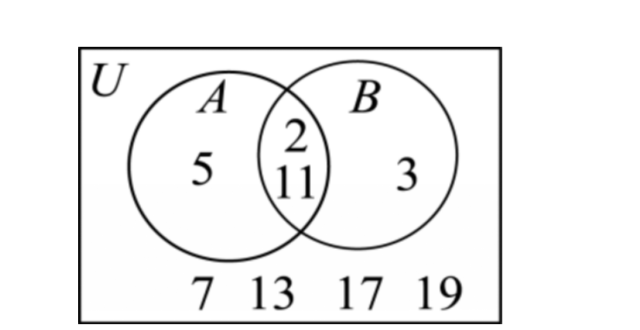
\includegraphics[width=0.24\textwidth]{figures/gao108_q6.png}
\end{center}

\solend
\fi

\item 若 $x\in A$，则 $\dfrac1x\in A$，就称 $A$ 自倒集合，集合 $M=\left\{-2,-1,0,\dfrac12,\dfrac13,1,2,3,4\right\}$ 的所有非空
子集中，自倒集合的个数为\blankline[4.4em].

\ifanswer
\solbegin
\step{由新定义，集合 $M$ 中的元素 1 和 $-1$ 倒数等于本身，2 和 $\dfrac12$，3 和 $\dfrac13$ 互为倒数,}
\step{故满足条件的自倒集合与集合 $\{-1,1,2,3\}$ 的非空子集的个数相同,}
\step{则其个数为 $2^4-1=15$.}
\solend
\fi

\item 设集合 $M=\{(x,y)\mid y=x^2+2bx+1\}$，$N=\{(x,y)\mid y=x+b\}(b\in\R)$，若
$M\cap N=\varnothing$，则实数 $b$ 的取值范围为\blankline[4.4em].

\ifanswer
\solbegin
\step{因为 $M\cap N=\varnothing$，所以
$\begin{cases}y=x^2+2bx+1\\y=x+b\end{cases}$
无解，则 $x^2+(2b-1)x+(1-b)=0$,}
\step{则 $\triangle=(2b-1)^2-4\times1\times(1-b)=4b^2-3<0$，解得 $-\dfrac{\sqrt3}2<b<\dfrac{\sqrt3}2$,}
\step{即实数 $b$ 的取值范围为 $\left(-\dfrac{\sqrt3}2,\dfrac{\sqrt3}2\right)$.}
\solend
\fi

\item 已知集合 $A=\left\{x\,\middle|\,\dfrac{x-a}{x^2-1}=1\right\}$ 有唯一元素，用列举法表示满足集合 $A$ 的条件的 $a$ 的取值集
合\blankline[4.4em].

\ifanswer
\solbegin
\step{$a=1$,$\dfrac{1}{x+1}=1$，一解；$a=-1$,$\dfrac{1}{x-1}=1$，一解；}
\step{$x-a=x^2-1$，一解时，$a=\dfrac54$,}
\step{综上，$a$ 的取值集合为 $\left\{-1,1,\dfrac54\right\}$.}
\solend
\fi

\item 已知集合 $M$ 的元素均为正整数，定义集合 $M$ 的“变项和”为：将 $M$ 中每个元素 $m$ 都乘
以 $(-1)^n$ 后再求和. 若集合 $A=\{n\mid1\leqslant n\leqslant2026,n\in\N\}$，则集合 $A$ 的所有非空子集的“变
项和”的总和为\blankline[4.4em].% $n$ 未加界定（据解析为元素序号），照录

\ifanswer
\solbegin
\step{$A=\{n\mid1\leqslant n\leqslant2026,n\in\N\}=\{1,2,\cdots,2026\}$,}
\step{1 在所有非空子集中共出现 $C_{2025}^{0}+C_{2025}^{1}+\cdots+C_{2025}^{2025}=2^{2025}$ 次,}
\step{同理 $2,3,\cdots,2026$ 都出现 $2^{2025}$ 次,}
\step{则集合 $A$ 的所有非空子集的“变项和”的总和}
\step{为 $2^{2025}\times[1\times(-1)^1+2\times(-1)^2+\cdots+2026\times(-1)^{2026}]$}
\step{$=2^{2025}\times(-1+2-3+4-\cdots-2025+2026)=1013\times2^{2025}$.}
\solend
\fi

\item 已知 $0<k<2$，定义 $[x]$ 为不超过 $x$ 的最大整数，区间 $[a,b]$（或 $(a,b)$，$[a,b)$，
$(a,b]$）的长度记为 $b-a$. 若关于 $x$ 的不等式 $k[x]>\lvert2[x]-6\rvert$ 的解集对应区间的长度为 $2$，
则 $k$ 的取值范围是\blankline[4.4em].

\ifanswer
\solbegin
\stepm{法一：}{由题意得 $\lvert2[x]-6\rvert=
\begin{cases}2[x]-6,x\geqslant3\\-2[x]+6,x<3\end{cases}$.}
\step{①当 $x\geqslant3$ 时，不等式 $k[x]>\lvert2[x]-6\rvert$ 可化为 $k[x]>2[x]-6$,}
\step{即 $(2-k)[x]<6$,}
\step{当 $0<k<2$ 时，解不等式 $(2-k)[x]<6$ 得 $[x]<\dfrac6{2-k}$.}
\step{②当 $x<3$ 时，不等式 $k[x]>\lvert2[x]-6\rvert$ 可化为 $k[x]>-2[x]+6$,}
\step{即 $(k+2)[x]>6$.}
\step{当 $0<k<2$ 时，解不等式 $(k+2)[x]>6$ 得 $[x]>\dfrac6{k+2}$.}
\step{综上所述，不等式 $k[x]>\lvert2[x]-6\rvert$ 的解集需满足 $\dfrac6{k+2}<[x]<\dfrac6{2-k}$,}
\step{由题意得在区间 $\left[\dfrac6{k+2},\dfrac6{2-k}\right]$ 内有两个整数,}
\step{由于 $\dfrac6{k+2}\in\left(\dfrac32,3\right)$，所以 $\dfrac6{2-k}\leqslant5$，得 $k\leqslant\dfrac45$.}
\step{因此 $k\in\left(0,\dfrac45\right]$，得 $\dfrac6{k+2}\in\left[\dfrac75,3\right)$，$\dfrac6{2-k}\in(3,5]$,}
\step{区间 $\left[\dfrac6{k+2},\dfrac6{2-k}\right]$ 内的两个整数是 3、4，所以 $4<\dfrac6{2-k}\leqslant5$，解得 $\dfrac12<k\leqslant\dfrac45$,}
\step{即 $k\in\left(\dfrac12,\dfrac45\right]$.}
\stepm{法二：}{令 $f(x)=kx$，$g(x)=\lvert2x-6\rvert$，画出 $g(x)$、$f(x)$ 的图象,}
\step{由于不等式 $k[x]>\lvert2[x]-6\rvert$ 的解集对应区间的长度为 2,}
\step{因此解集只可能为 $[3,5)$ 或 $[2,4)$.}
\step{当解集为 $[3,5)$ 时，如图（2），数形结合易得
$\begin{cases}f(2)\leqslant g(2)\\f(4)>g(4)\\f(5)\leqslant g(5)\end{cases}$,}
\step{即
$\begin{cases}2k\leqslant\lvert2\times2-6\rvert\\4k>\lvert2\times4-6\rvert\\5k\leqslant\lvert2\times5-6\rvert\end{cases}$，
解得
$\begin{cases}k\leqslant1\\k>\dfrac12\\k\leqslant\dfrac45\end{cases}$，
所以 $\dfrac12<k\leqslant\dfrac45$，满足 $0<k<2$,}
\step{当解集为 $[2,4)$ 时，如图（1），数形结合易得
$\begin{cases}f(2)>g(2)\\f(4)\leqslant g(4)\end{cases}$,}
\step{即
$\begin{cases}2k>\lvert2\times2-6\rvert\\4k\leqslant\lvert2\times4-6\rvert\end{cases}$，
无解.}

\begin{center}
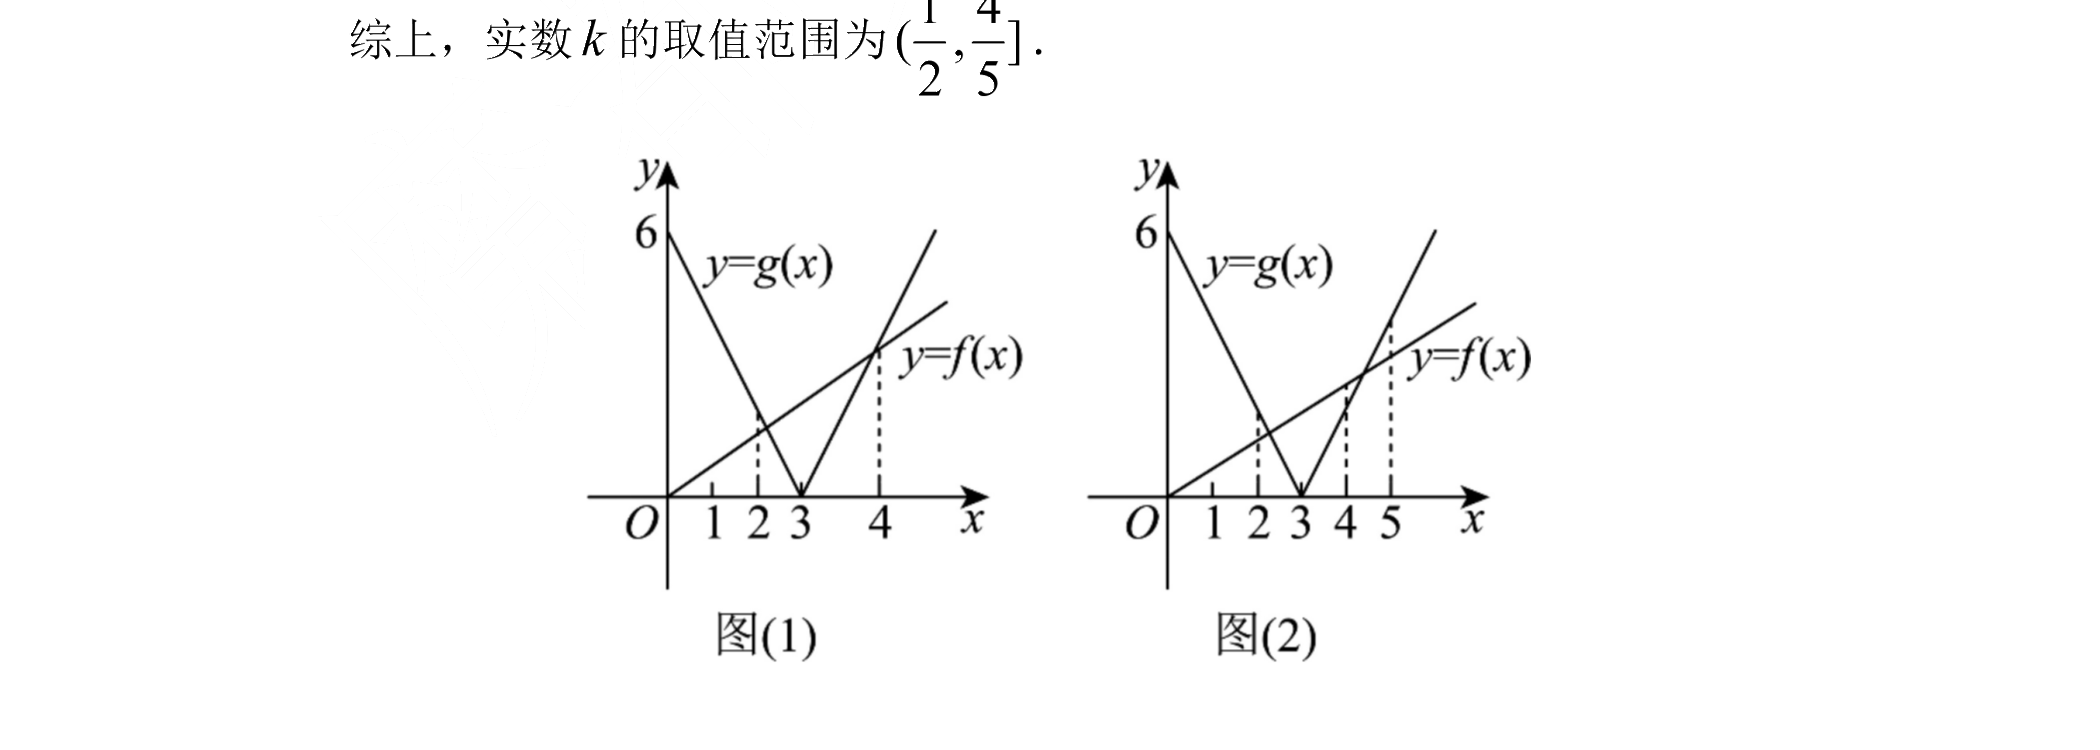
\includegraphics[width=0.72\textwidth]{figures/gao108_q11.png}
\end{center}

\step{综上，实数 $k$ 的取值范围为 $\left(\dfrac12,\dfrac45\right]$.}
\solend
\fi

\item 已知集合 $A=[1,a]\cup[a^3,a^4]$，集合 $B=\{x\mid x=x_1-x_2$，其中 $x_1$,$x_2\in A\}$. 若集合 $B$ 表
示的区间为一个闭区间，则实数 $a$ 的取值范围为\blankline[4.4em].

\ifanswer
\solbegin
\step{由题意得 $a^3>a>1$，则 $x_1-x_2$ 的最小值为 $1-a^4$，最大值为 $a^4-1$,}
\step{所以 $B=[1-a^4,a^4-1]$,}
\step{又因为 $a^4-a^3-(a-1)=a^3(a-1)-(a-1)=(a^3-1)(a-1)>0$,}
\step{所以 $a^4-a^3>a-1$，又集合 $B$ 表示的区间为一个闭区间,}
\step{则 $a^3-a\leqslant a^4-a^3$，化简得 $a^2-a-1\geqslant0$，又 $a>1$，解得 $a\geqslant\dfrac{1+\sqrt5}2$.}
\solend
\fi

\end{enumerate}

\bigsec{二、选择题}

\begin{enumerate}
\setcounter{enumi}{12}

\item 若 $a,b,c\in\R$，则下列不等式恒成立的是\mbox{（\quad）}% 原卷把答案“C”印在题干括号内、无【解析】

\keepwithprev
A. $\dfrac1a<\dfrac1b$\qquad B. $a^2<b^2$\qquad C. $\dfrac{a}{c^2+1}>\dfrac{b}{c^2+1}$\qquad D. $a\lvert c\rvert>b\lvert c\rvert$

\ifanswer
\ans{$C$}
\fi

\item 以下几个关系中正确的是\mbox{（\quad）}

\keepwithprev
A. $0\in\varnothing$\qquad\qquad\qquad B. $\varnothing\in\{x\mid x^2+1=0\}$

C. $\varnothing\subset\{0\}$\qquad\qquad\qquad D. $(A\cap B)\subset(A\cup B)$

\ifanswer
\solbegin
\step{$A$ 选项，$\varnothing$ 不包含任何元素，所以 $0\in\varnothing$ 错误，$A$ 错,}
\step{$B$ 选项，集合与集合之间关系不可以用 $\in$，$B$ 错,}
\step{$C$ 选项，空集是非空集合的真子集，所以 $\varnothing\subset\{0\}$ 正确，$C$ 对,}
\step{$D$ 选项，当 $A=B$ 时，$(A\cap B)=(A\cup B)$，$D$ 错,}
\step{故选 $C$.}
\solend
\fi

\item 设全集为 $U$，图中阴影部分所表示的集合是\mbox{（\quad）}% 原卷把答案“A”印在题干括号内、无【解析】

\keepwithprev
A. $B\cap\overline{A\cup C}$\qquad\qquad B. $(A\cup B)\cap(B\cup C)$

C. $(A\cup C)\cap\overline B$\qquad\qquad D. $(\overline A\cup\overline C)\cap B$

\ifanswer
\ans{$A$}
\fi

\item 对于 $k=0,1,2,\cdots$，定义集合 $A_k=\{20+k,26+2k\}$，并记 $S_k=A_0\cup A_1\cup\cdots\cup A_k$，则
使得集合 $S_n$ 中完全平方数的个数为奇数的最小正整数 $n$ 为\mbox{（\quad）}

\keepwithprev
A. $18$\qquad\qquad B. $19$\qquad\qquad C. $20$\qquad\qquad D. $21$

\ifanswer
\solbegin
\step{当 $k=0$ 时，$A_0=\{20,26\}$，对于 $k=0,1,2,\cdots$,}
\step{集合 $A_k$ 中最小的元素 $20>4^2$，若 $S_n$ 中完全平方数的个数为奇数，则 $n>4$,}
\step{（1）$20+k=5^2$ 时，$k=5$，$A_5=\{25,36\}$，此时 $S_5$ 中完全平方数为 $5^2$、$6^2$,}
\step{个数为 2;}
\step{$20+k=6^2$ 时，$k=16$，$A_{16}=\{36,58\}$，此时 $S_{16}$ 中完全平方数为 $5^2$、$6^2$,}
\step{个数为 2;}
\step{$20+k=7^2$ 时，$k=29$，$A_{29}=\{49,84\}$,}
\step{此时 $S_{29}$ 中完全平方数为 $5^2$、$6^2$、$7^2$、$8^2$，个数为 4;}
\step{$20+k=8^2$ 时，$k=44$，$A_{44}=\{64,114\}$,}
\step{此时 $S_{44}$ 中完全平方数为 $5^2$、$6^2$、$7^2$、$8^2$、$10^2$，个数为 5;}
\step{（2）因为 $k=0,1,2,\cdots,26+2k$ 一定为偶数,}
\step{所以 $26+2k=6^2$ 时，$k=5$，由上述分析得 $S_5$ 中完全平方数个数为 2;}
\step{$26+2k=8^2$ 时，$k=19$，$A_{19}=\{39,64\}$,}
\step{此时 $S_{19}$ 中完全平方数为 $5^2$、$6^2$、$8^2$，个数为 3.}
\step{综上，使集合 $S_n$ 中完全平方数的个数为奇数的最小正整数 $n=19$. 故选 $B$.}
\solend
\fi

\end{enumerate}

\bigsec{三、解答题}

\begin{enumerate}
\setcounter{enumi}{16}

\item 设全集 $U=\R$，集合 $A=\left\{x\,\middle|\,\dfrac{x-2}{x+2}\leqslant0\right\}$，$B=\{x\mid a\leqslant x<2a+1,a\in\R\}$，
$C=\{x\mid\lvert2x-1\rvert<5\}$.

（1）求集合 $A$、$\overline A\cup C$；

（2）若 $B\subseteq A$，求实数 $a$ 的取值范围.

\ifanswer
\solbegin
\ansspace*
\step{（1）不等式 $\dfrac{x-2}{x+2}\leqslant0$，等价于
$\begin{cases}(x-2)(x+2)\leqslant0\\x+2\neq0\end{cases}$，
解得 $\{x\mid-2<x\leqslant2\}$,}
\step{所以 $A=\{x\mid-2<x\leqslant2\}$，则 $\overline A=\{x\mid x\leqslant-2$ 或 $x>2\}$,}
\step{因为 $C=\{x\mid\lvert2x-1\rvert<5\}=\{x\mid-2<x<3\}$，所以 $\overline A\cup C=\R$；}
\step{（2）因为 $B\subseteq A$,}
\step{若 $B=\varnothing$，则 $a\geqslant2a+1$，解得 $a\leqslant-1$,}
\step{若 $B\neq\varnothing$，则
$\begin{cases}a<2a+1\\a>-2\\2a+1\leqslant2\end{cases}$，
解得 $-1<a\leqslant\dfrac12$,}
\step{综上所述，实数 $a$ 的取值范围为 $\left\{a\,\middle|\,a\leqslant\dfrac12\right\}$.}
\solend
\fi

\item 设 $a$、$b$、$c$、$d$ 是四个正数.

（1）已知 $a>b$，比较 $\dfrac{2a+b}{a+2b}$ 与 $\dfrac ab$ 的值的大小；

（2）若 $(1+a)(1+b)(1+c)(1+d)<16$，求证：$a$、$b$、$c$、$d$ 中至少有一个小于 1.

\ifanswer
\solbegin
\step{（1）$\dfrac{2a+b}{a+2b}-\dfrac ab=\dfrac{b^2-a^2}{b(a+2b)}<0$，所以 $\dfrac{2a+b}{a+2b}<\dfrac ab$.}
\step{（2）假设 $a$、$b$、$c$、$d$ 都不小于 1，即 $a$、$b$、$c$、$d$ 均大于等于 1,}
\step{即 $a\geqslant1$，$b\geqslant1$，$c\geqslant1$，$d\geqslant1$,}
\step{由均值不等式得 $1+a\geqslant2\sqrt a$,$1+b\geqslant2\sqrt b$,$1+c\geqslant2\sqrt c$,$1+d\geqslant2\sqrt d$,}
\step{故 $(1+a)(1+b)(1+c)(1+d)\geqslant16\sqrt{abcd}\geqslant16$,}
\step{当且仅当 $a=b=c=d=1$ 时取等号,}
\step{这与 $(1+a)(1+b)(1+c)(1+d)<16$ 矛盾，故假设不成立，原命题成立.}
\solend
\fi

\item 已知 $m\in\R$，一个二次项系数为 1 的一元二次方程的两个不等实根分别为 $x_1$ 和 $x_2$，且
满足
$\begin{cases}x_1^2+x_2^2=2m^2-4\\x_1+x_2=m\end{cases}$.

（1）直接写出该一元二次方程；

（2）若 $(3x_1-x_2)(3x_2-x_1)\geqslant-1$，求 $m$ 的取值范围；

（3）若方程的两根 $x_1$ 和 $x_2$ 都大于 $-1$，求 $m$ 的取值范围.

\ifanswer
\solbegin
\step{（1）设这个一元二次方程为 $x^2+bx+c=0$,}
\step{由
$\begin{cases}x_1^2+x_2^2=2m^2-4\\x_1+x_2=m\end{cases}$,}
\step{得 $(x_1+x_2)^2=x_1^2+x_2^2+2x_1x_2=2m^2-4+2x_1x_2=m^2$，即 $x_1x_2=\dfrac{4-m^2}2$,}
\step{由韦达定理得 $x_1+x_2=-b=m$，即 $x_1x_2=c=\dfrac{4-m^2}2$,}
\step{所以一元二次方程为 $x^2-mx+\dfrac{4-m^2}2=0$.}
\step{（2）$(3x_1-x_2)(3x_2-x_1)=9x_1x_2-3x_1^2-3x_2^2+x_1x_2=10x_1x_2-3(x_1^2+x_2^2)\geqslant-1$,}
\step{结合已知及（1）得 $x_1^2+x_2^2=2m^2-4$,$x_1x_2=\dfrac{4-m^2}2$,}
\step{代入得 $10\times\dfrac{4-m^2}2-3(2m^2-4)=-11m^2+32\geqslant-1\Rightarrow m^2\leqslant3$}
\step{$\Rightarrow-\sqrt3\leqslant m\leqslant\sqrt3$,}
\step{又 $\Delta=m^2-4\times\dfrac{4-m^2}2=3m^2-8>0\Rightarrow m<-\dfrac{2\sqrt6}3$ 或 $m>\dfrac{2\sqrt6}3$,}
\step{所以 $m\in\left[-\sqrt3,-\dfrac{2\sqrt6}3\right)\cup\left(\dfrac{2\sqrt6}3,\sqrt3\right]$.}
\step{（3）若方程的两根 $x_1$ 和 $x_2$ 都大于 $-1$，则
$\begin{cases}\Delta>0\\x_1+x_2>-2\\(x_1+1)(x_2+1)>0\end{cases}$,}
\step{所以
$\begin{cases}\Delta=3m^2-8>0\\m>-2\\[2pt]\dfrac{4-m^2}2+m+1>0\end{cases}$，
解得 $m\in\left(1-\sqrt7,-\dfrac{2\sqrt6}3\right)\cup\left(\dfrac{2\sqrt6}3,1+\sqrt7\right)$.}
\solend
\fi

\item 已知不等式 $2\leqslant ax^2+bx+c\leqslant3$ 的解集为 $\{x\mid2\leqslant x\leqslant3\}$.

（1）若 $a>0$，求 $6b+5c$ 的值；

（2）若 $a>0$，且不等式 $ax^2+(b-3)x-c\leqslant0$ 有且仅有 9 个整数解，求 $a$ 的取值范围；

（3）若 $a<0$，对任意的 $x<0$，不等式 $(ax-4)(x^2+b+c+1)\geqslant0$ 恒成立，求 $a^2-b+c$
的取值集合.

\ifanswer
\solbegin
\ansspace*
\step{（1）$a>0$,}
\step{结合二次函数图象得不等式 $ax^2+bx+c\leqslant3$ 的解集为 $\{x\mid2\leqslant x\leqslant3\}$,}
\step{且不等式 $ax^2+bx+c\geqslant2$ 的解集为 $R$,}
\step{所以方程 $ax^2+bx+c-3=0$ 的两根分别为 2 和 3,}
\step{则
$\begin{cases}2+3=-\dfrac ba\\[2pt]2\times3=\dfrac{c-3}a\end{cases}$，
得 $b=-5a$，$c=6a+3$,}
\step{所以 $6b+5c=6\times(-5a)+5(6a+3)=15$.}
\step{（2）若 $a>0$，且不等式 $ax^2+(b-3)x-c\leqslant0$ 有且仅有 9 个整数解,}
\step{由（1）得 $b=-5a$，$c=6a+3$,}
\step{不等式 $ax^2+bx+c\geqslant2$ 可化为 $ax^2-5ax+6a+1\geqslant0$.}
\step{由（1）得不等式 $ax^2+bx+c\geqslant2$ 的解集为 $R$,}
\step{所以 $ax^2-5ax+6a+1\geqslant0$ 恒成立,}
\step{所以
$\begin{cases}a>0\\\Delta=25a^2-4a(6a+1)\leqslant0\end{cases}$，
即
$\begin{cases}a>0\\a^2-4a=a(a-4)\leqslant0\end{cases}$，}
\step{解得 $0<a\leqslant4$.}
\step{不等式 $ax^2+(b-3)x-c\leqslant0$ 等价于 $ax^2-(5a+3)x-(6a+3)\leqslant0$,}
\step{所以 $[ax-(6a+3)](x+1)\leqslant0$，得 $-1\leqslant x\leqslant6+\dfrac3a$,}
\step{所以 $7\leqslant6+\dfrac3a<8$，解得 $\dfrac32<a\leqslant3$.}
\step{综上，$a$ 的取值范围为 $\left(\dfrac32,3\right]$.}
\step{（3）因为 $a<0$,}
\step{同（1）分析，不等式 $ax^2+bx+c\geqslant2$ 的解集为 $\{x\mid2\leqslant x\leqslant3\}$,}
\step{$ax^2+bx+c\leqslant3$ 的解集为 $R$,}
\step{所以方程 $ax^2+bx+c-2=0$ 的两根分别为 2 和 3,}
\step{则
$\begin{cases}2+3=-\dfrac ba\\[2pt]2\times3=\dfrac{c-2}a\end{cases}$，
得 $b=-5a$，$c=6a+2$.}
\step{所以不等式 $ax^2+bx+c=ax^2-5ax+6a+2\leqslant3$ 的解集为 $R$,}
\step{则 $ax^2-5ax+6a-1\leqslant0$ 恒成立,}
\step{所以
$\begin{cases}a<0\\\Delta=25a^2-4a(6a-1)\leqslant0\end{cases}$，
即
$\begin{cases}a<0\\a^2+4a=a(a+4)\leqslant0\end{cases}$，}
\step{解得 $-4\leqslant a<0$.}
\step{所以对任意的 $x<0$，不等式 $(ax-4)(x^2+b+c+1)\geqslant0$ 恒成立}
\step{转化为对任意的 $x<0$，不等式 $(ax-4)(x^2+a+3)\geqslant0$ 恒成立.}
\step{方程 $(ax-4)(x^2+a+3)=0$ 的两个根为 $x=\dfrac4a<0$,}
\step{$x=\pm\sqrt{-a-3}$（$a<-3$ 时成立）,}
\step{因而仅当 $ax-4=0$ 与 $x^2+a+3=0$ 的负根重合时满足条件,}
\step{解得唯一解为 $a=-4$，所以 $a^2-b+c=a^2+11a+2=-26$,}
\step{所以 $a^2-b+c$ 的取值集合为 $\{-26\}$.}
\solend
\fi

\item 已知集合 $A=\{1,2,3,4,5,6,7,8\}$，$M=\{(x,y)\mid x\in A,y\in A\}$，从 $M$ 中选取 $n$ 个不同的
元素组成一个序列：$(x_1,y_1)$,$(x_2,y_2),\cdots,(x_n,y_n)$，其中 $(x_i,y_i)$ 称为该序列的第 $i$ 项
（$i=1,2,\cdots,n$），若该序列的相邻项 $(x_i,y_i)$,$(x_{i+1},y_{i+1})$ 满足：
\[\begin{cases}\lvert x_{i+1}-x_i\rvert=3\\\lvert y_{i+1}-y_i\rvert=4\end{cases}
\quad\text{或}\quad
\begin{cases}\lvert x_{i+1}-x_i\rvert=4\\\lvert y_{i+1}-y_i\rvert=3\end{cases}\]
（$i=1,2,\cdots,n-1$），则称该序列为“$\Delta-$序列”.

（1）若一个 $\Delta-$序列的第一项为 $(4,4)$，请直接写出它所有可能的第二项；

（2）定义集合 $A=\{1,2,3,4,5,6,7,8\}$ 的两个子集：外侧集 $S=\{1,2,7,8\}$，内侧集
$T=\{3,4,5,6\}$. 证明：若 $\Delta-$序列中某一项的坐标在区域 $S\times S$ 内（即横、纵坐标均属于
$S$），则它的下一项坐标必定在区域 $T\times T$ 内；

（3）证明：不存在一个恰好有 5 项的 $\Delta-$序列，使其第一项为 $(1,8)$，且第五项为
$(8,1)$.

\ifanswer
\solbegin
\ansspace*
\step{（1）由题意，第一项为 $(x_1,y_1)=(4,4)$,}
\step{对于第二项 $(x_2,y_2)$，其坐标必须在 1~8 之间.}
\step{若 $\lvert x_2-4\rvert=3$,$\lvert y_2-4\rvert=4$，则 $x_2\in\{1,7\}$,}
\step{且 $y_2\in\{8\}$（因为 $4-4=0$ 不在集合 $A$ 中）. 此时可能的点为 $(1,8)$,$(7,8)$.}
\step{若 $\lvert x_2-4\rvert=4$,$\lvert y_2-4\rvert=3$，则 $x_2\in\{8\}$，且 $y_2\in\{1,7\}$.}
\step{此时可能的点为 $(8,1)$,$(8,7)$.}
\step{所以它所有可能的第二项为 $(1,8)$,$(7,8)$,$(8,1)$,$(8,7)$.}
\step{（2）已知某一项 $(x_t,y_t)\in S\times S$，即 $x_t\in\{1,2,7,8\}$ 且 $y_t\in\{1,2,7,8\}$.}
\step{由规则得下一步坐标的变化量为 3 和 4，设 $a\in S$ 变化 3 或 4 后的结果 $a'$:}
\step{当 $a=1$ 时，$1+3=4\in T$,$1+4=5\in T$；}
\step{当 $a=2$ 时，$2+3=5\in T$,$2+4=6\in T$；}
\step{当 $a=7$ 时，$7-3=4\in T$,$7-4=3\in T$；}
\step{当 $a=8$ 时，$8-3=5\in T$,$8-4=4\in T$.}
\step{（注：由于超出 1~8 范围的越界坐标不符合.）}
\step{由此可见，无论 $a$ 是 $S$ 中的哪一个数，加上或减去 3 或 4 之后,}
\step{得到的新坐标必属于集合 $T$.}
\step{因为 $\Delta-$序列每走一步，横坐标和纵坐标必定同时发生 3 和 4 的变化,}
\step{所以新的横坐标 $x_{i+1}$ 必属于 $T$，新的纵坐标 $y_{i+1}$ 也必属于 $T$,}
\step{即下一项 $(x_{i+1},y_{i+1})$ 必定在区域 $T\times T$ 内. ………10 分原命题得证.% 得分行混入证明，照录
}
\step{（3）假设存在这样一个包含 5 项的 $\Delta-$序列:}
\step{$(x_1,y_1)$,$(x_2,y_2)$,$(x_3,y_3)$,$(x_4,y_4)$,$(x_5,y_5)$.}
\step{已知第一项为 $(1,8)$，第五项为 $(8,1)$. 第 2 项必须是第 1 项 $(1,8)$ 的相邻点.}
\step{我们来找 $(1,8)$ 的相邻点：第 2 项只能是 $(4,4)$ 或 $(5,5)$,}
\step{第 4 项必须是第 5 项 $(8,1)$ 的相邻点（因为跳跃是双向可逆的）.}
\step{同理可算得，$(8,1)$ 的相邻点也只有两个：$(4,4)$ 和 $(5,5)$,}
\step{题目题干中明确规定，$\Delta-$序列由 $n$ 个不同的有序数对构成.% “题目题干”措辞重复，照录
}
\step{所以，第 2 项和第 4 项不能是同一个点. 这就意味着:}
\step{如果第 2 项是 $(4,4)$，第 4 项就必须是 $(5,5)$；反之亦然.}
\step{则第 3 项必须是 $(4,4)$ 和 $(5,5)$ 的公共相邻点.}
\step{$(4,4)$ 的相邻点集合为：$\{(1,8),(7,8),(8,1),(8,7)\}$,}
\step{$(5,5)$ 的相邻点集合为：$\{(2,1),(8,1),(1,2),(1,8)\}$,}
\step{所以，第 3 项只能填 $(1,8)$ 或者 $(8,1)$.}
\step{这与“序列由不同的有序数对构成”这一条件产生矛盾！}
\step{所以，不存在一个恰好有 5 项的 $\Delta-$序列,}
\step{使其第一项为 $(1,8)$，且第五项为 $(8,1)$.}
\solend
\fi

\end{enumerate}

\end{document}
"
%
% 原始材料：微信公众号“魔都数学加油站”文章，作者破晓，2026-11-03 17:19 发布；
% 连载“27学年高一108”，原文标题“27学年高一108——2026-2027年上海市五校联考高一上10月月考”；
% 原文链接：https://mp.weixin.qq.com/s/3nkP789Qar93NGMZXFFCSw。
% 正文为 14 张 PNG 页（第 2、3、6—13 页 4762×6735，第 1、4、5、14 页 2560×3620），
% 题目下印有【解析】，为讲评版。
% 题目、解析均据原图转录；卷面水印及公众号页脚未录入。
% 第 6 题解析的文氏图与第 11 题法二解析的两幅图象（图(1)、图(2)）裁自原图、去粉色水印
% 转灰度（gao108_q6.png、gao108_q11.png），第 6 题图属解析（仅答案版）、
% 第 11 题图属解析（仅答案版）。
%
% 卷首标题：原卷印作“2026-2027 年五校联考高一上 10 月月考”，标题下另印一行参与学校
% 名单“闵行中学、嘉定一中、松江一中、金山中学、嘉一实高”（全稿第 5 份原卷自印副标题，
% 按 14／24／49／50 成例照录，并登记进计数核对.py 的 SELFSUB）。
%
% 与原卷的排版差异：
%   ① 原文从第 3 题起，填空题编号为 3—12、选择题为 13—16、解答题为 17—21，本稿保留原题号；
%   ② 原卷每题下直接印【解析】，本稿按全稿惯例将解析置于答案版；第 4 题只印【答案】，
%      第 13、15 两题把答案印在题干括号内且无【解析】，均另提 \ans{}；
%   ③ 原卷副标题照录（见上）；
%   ④ 原卷填空横线按全稿惯例排为 \blankline[4.4em]；解答题按惯例加 \ansspace；选择题括号排
%      \mbox{（\quad）}、选项段前按惯例加 \keepwithprev；
%   ⑤ 原卷数集排斜体 $R$／$N$，按全稿惯例改 \R、\N。
%
% 原卷红色强调照录为黑体：第 11 题解析的“法一：”“法二：”原卷排红色，按 53 成例排
% \stepm{法一：}／\stepm{法二：}（加粗着色）。
%
% 原卷存疑：第 10 题题干“变项和”定义中“将 $M$ 中每个元素 $m$ 都乘以 $(-1)^n$ 后再求和”
% 的 $n$ 未加界定（据解析应为该元素在 $\{1,2,\cdots,2026\}$ 中的序号），照录。
% 第 21 题 (2) 解析末行“即下一项 $(x_{i+1},y_{i+1})$ 必定在区域 $T\times T$ 内. ………10 分
% 原命题得证.”，原卷把得分点行混入证明（“原命题”按上下文为“原命题的逆否”），照录。
% 第 21 题 (3) 解析“题目题干中明确规定”，“题目题干”措辞重复，照录。
%
% 行数核对：逐题数 \step/\stepm 条数，合计 164 条（Q3：3；Q4：0；Q5：2；Q6：1；Q7：3；
% Q8：3；Q9：3；Q10：6；Q11：21；Q12：5；Q13：0；Q14：5；Q15：0；Q16：15；Q17：7；
% Q18：7；Q19：13；Q20：34；Q21：36），与原卷印刷行逐题相等。第 4 题只印【答案】、
% 第 13、15 题括号内印答案，均提 \ans{}，不计入 \step 账。
%
\documentclass[a4paper,11pt]{article}
\usepackage{common}

\begin{document}

\examtitlest[3]{2026--2027 年五校联考高一上 10 月月考}{闵行中学、嘉定一中、松江一中、金山中学、嘉一实高}

\bigsec{一、填空题}

\begin{enumerate}
\setcounter{enumi}{2}

\item 已知等式 $2x^2+3x+5=2ax^2+a(3x+1)+c$ 恒成立，则实数 $a+c$ 的值为\blankline[4.4em].

\ifanswer
\solbegin
\step{因为 $2x^2+3x+5=2ax^2+a(3x+1)+c$ 恒成立,}
\step{即 $2x^2+3x+5=2ax^2+3ax+(a+c)$ 恒成立，所以
$\begin{cases}2=2a\\3=3a\\5=a+c\end{cases}$,}
\step{所以 $a+c=5$.}
\solend
\fi

\item 不等式 $\dfrac1x<\dfrac12$ 的解集是\blankline[4.4em].

\ifanswer
\ans{$(-\infty,0)\cup(2,+\infty)$}
\fi

\item 已知 $a$、$b$ 都是实数，则“$a^2=b^2$”是“$a^2+b^2=2ab$”的\blankline[4.4em]条件.

\ifanswer
\solbegin
\step{$a^2=b^2$ 等价于 $a=\pm b$；$a^2+b^2=2ab$ 等价于 $(a-b)^2=0$ 等价于 $a=b$,}
\step{故“$a^2=b^2$”是“$a^2+b^2=2ab$”的必要不充分条件.}
\solend
\fi

\item 已知全集 $U=\{x\mid x$ 为不大于 20 的素数$\}$，$A\cap\overline B=\{5\}$，$\overline A\cap B=\{3\}$，
$\overline{A\cup B}=\{7,13,17,19\}$，则 $A=$\blankline[4.4em].

\ifanswer
\solbegin
\step{如图所示，$A=\{2,5,11\}$.}

\begin{center}
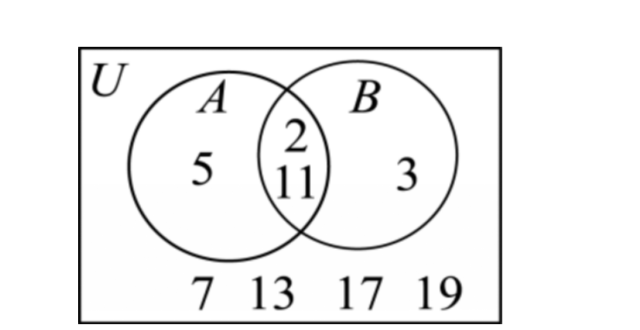
\includegraphics[width=0.24\textwidth]{figures/gao108_q6.png}
\end{center}

\solend
\fi

\item 若 $x\in A$，则 $\dfrac1x\in A$，就称 $A$ 自倒集合，集合 $M=\left\{-2,-1,0,\dfrac12,\dfrac13,1,2,3,4\right\}$ 的所有非空
子集中，自倒集合的个数为\blankline[4.4em].

\ifanswer
\solbegin
\step{由新定义，集合 $M$ 中的元素 1 和 $-1$ 倒数等于本身，2 和 $\dfrac12$，3 和 $\dfrac13$ 互为倒数,}
\step{故满足条件的自倒集合与集合 $\{-1,1,2,3\}$ 的非空子集的个数相同,}
\step{则其个数为 $2^4-1=15$.}
\solend
\fi

\item 设集合 $M=\{(x,y)\mid y=x^2+2bx+1\}$，$N=\{(x,y)\mid y=x+b\}(b\in\R)$，若
$M\cap N=\varnothing$，则实数 $b$ 的取值范围为\blankline[4.4em].

\ifanswer
\solbegin
\step{因为 $M\cap N=\varnothing$，所以
$\begin{cases}y=x^2+2bx+1\\y=x+b\end{cases}$
无解，则 $x^2+(2b-1)x+(1-b)=0$,}
\step{则 $\triangle=(2b-1)^2-4\times1\times(1-b)=4b^2-3<0$，解得 $-\dfrac{\sqrt3}2<b<\dfrac{\sqrt3}2$,}
\step{即实数 $b$ 的取值范围为 $\left(-\dfrac{\sqrt3}2,\dfrac{\sqrt3}2\right)$.}
\solend
\fi

\item 已知集合 $A=\left\{x\,\middle|\,\dfrac{x-a}{x^2-1}=1\right\}$ 有唯一元素，用列举法表示满足集合 $A$ 的条件的 $a$ 的取值集
合\blankline[4.4em].

\ifanswer
\solbegin
\step{$a=1$,$\dfrac{1}{x+1}=1$，一解；$a=-1$,$\dfrac{1}{x-1}=1$，一解；}
\step{$x-a=x^2-1$，一解时，$a=\dfrac54$,}
\step{综上，$a$ 的取值集合为 $\left\{-1,1,\dfrac54\right\}$.}
\solend
\fi

\item 已知集合 $M$ 的元素均为正整数，定义集合 $M$ 的“变项和”为：将 $M$ 中每个元素 $m$ 都乘
以 $(-1)^n$ 后再求和. 若集合 $A=\{n\mid1\leqslant n\leqslant2026,n\in\N\}$，则集合 $A$ 的所有非空子集的“变
项和”的总和为\blankline[4.4em].% $n$ 未加界定（据解析为元素序号），照录

\ifanswer
\solbegin
\step{$A=\{n\mid1\leqslant n\leqslant2026,n\in\N\}=\{1,2,\cdots,2026\}$,}
\step{1 在所有非空子集中共出现 $C_{2025}^{0}+C_{2025}^{1}+\cdots+C_{2025}^{2025}=2^{2025}$ 次,}
\step{同理 $2,3,\cdots,2026$ 都出现 $2^{2025}$ 次,}
\step{则集合 $A$ 的所有非空子集的“变项和”的总和}
\step{为 $2^{2025}\times[1\times(-1)^1+2\times(-1)^2+\cdots+2026\times(-1)^{2026}]$}
\step{$=2^{2025}\times(-1+2-3+4-\cdots-2025+2026)=1013\times2^{2025}$.}
\solend
\fi

\item 已知 $0<k<2$，定义 $[x]$ 为不超过 $x$ 的最大整数，区间 $[a,b]$（或 $(a,b)$，$[a,b)$，
$(a,b]$）的长度记为 $b-a$. 若关于 $x$ 的不等式 $k[x]>\lvert2[x]-6\rvert$ 的解集对应区间的长度为 $2$，
则 $k$ 的取值范围是\blankline[4.4em].

\ifanswer
\solbegin
\stepm{法一：}{由题意得 $\lvert2[x]-6\rvert=
\begin{cases}2[x]-6,x\geqslant3\\-2[x]+6,x<3\end{cases}$.}
\step{①当 $x\geqslant3$ 时，不等式 $k[x]>\lvert2[x]-6\rvert$ 可化为 $k[x]>2[x]-6$,}
\step{即 $(2-k)[x]<6$,}
\step{当 $0<k<2$ 时，解不等式 $(2-k)[x]<6$ 得 $[x]<\dfrac6{2-k}$.}
\step{②当 $x<3$ 时，不等式 $k[x]>\lvert2[x]-6\rvert$ 可化为 $k[x]>-2[x]+6$,}
\step{即 $(k+2)[x]>6$.}
\step{当 $0<k<2$ 时，解不等式 $(k+2)[x]>6$ 得 $[x]>\dfrac6{k+2}$.}
\step{综上所述，不等式 $k[x]>\lvert2[x]-6\rvert$ 的解集需满足 $\dfrac6{k+2}<[x]<\dfrac6{2-k}$,}
\step{由题意得在区间 $\left[\dfrac6{k+2},\dfrac6{2-k}\right]$ 内有两个整数,}
\step{由于 $\dfrac6{k+2}\in\left(\dfrac32,3\right)$，所以 $\dfrac6{2-k}\leqslant5$，得 $k\leqslant\dfrac45$.}
\step{因此 $k\in\left(0,\dfrac45\right]$，得 $\dfrac6{k+2}\in\left[\dfrac75,3\right)$，$\dfrac6{2-k}\in(3,5]$,}
\step{区间 $\left[\dfrac6{k+2},\dfrac6{2-k}\right]$ 内的两个整数是 3、4，所以 $4<\dfrac6{2-k}\leqslant5$，解得 $\dfrac12<k\leqslant\dfrac45$,}
\step{即 $k\in\left(\dfrac12,\dfrac45\right]$.}
\stepm{法二：}{令 $f(x)=kx$，$g(x)=\lvert2x-6\rvert$，画出 $g(x)$、$f(x)$ 的图象,}
\step{由于不等式 $k[x]>\lvert2[x]-6\rvert$ 的解集对应区间的长度为 2,}
\step{因此解集只可能为 $[3,5)$ 或 $[2,4)$.}
\step{当解集为 $[3,5)$ 时，如图（2），数形结合易得
$\begin{cases}f(2)\leqslant g(2)\\f(4)>g(4)\\f(5)\leqslant g(5)\end{cases}$,}
\step{即
$\begin{cases}2k\leqslant\lvert2\times2-6\rvert\\4k>\lvert2\times4-6\rvert\\5k\leqslant\lvert2\times5-6\rvert\end{cases}$，
解得
$\begin{cases}k\leqslant1\\k>\dfrac12\\k\leqslant\dfrac45\end{cases}$，
所以 $\dfrac12<k\leqslant\dfrac45$，满足 $0<k<2$,}
\step{当解集为 $[2,4)$ 时，如图（1），数形结合易得
$\begin{cases}f(2)>g(2)\\f(4)\leqslant g(4)\end{cases}$,}
\step{即
$\begin{cases}2k>\lvert2\times2-6\rvert\\4k\leqslant\lvert2\times4-6\rvert\end{cases}$，
无解.}

\begin{center}
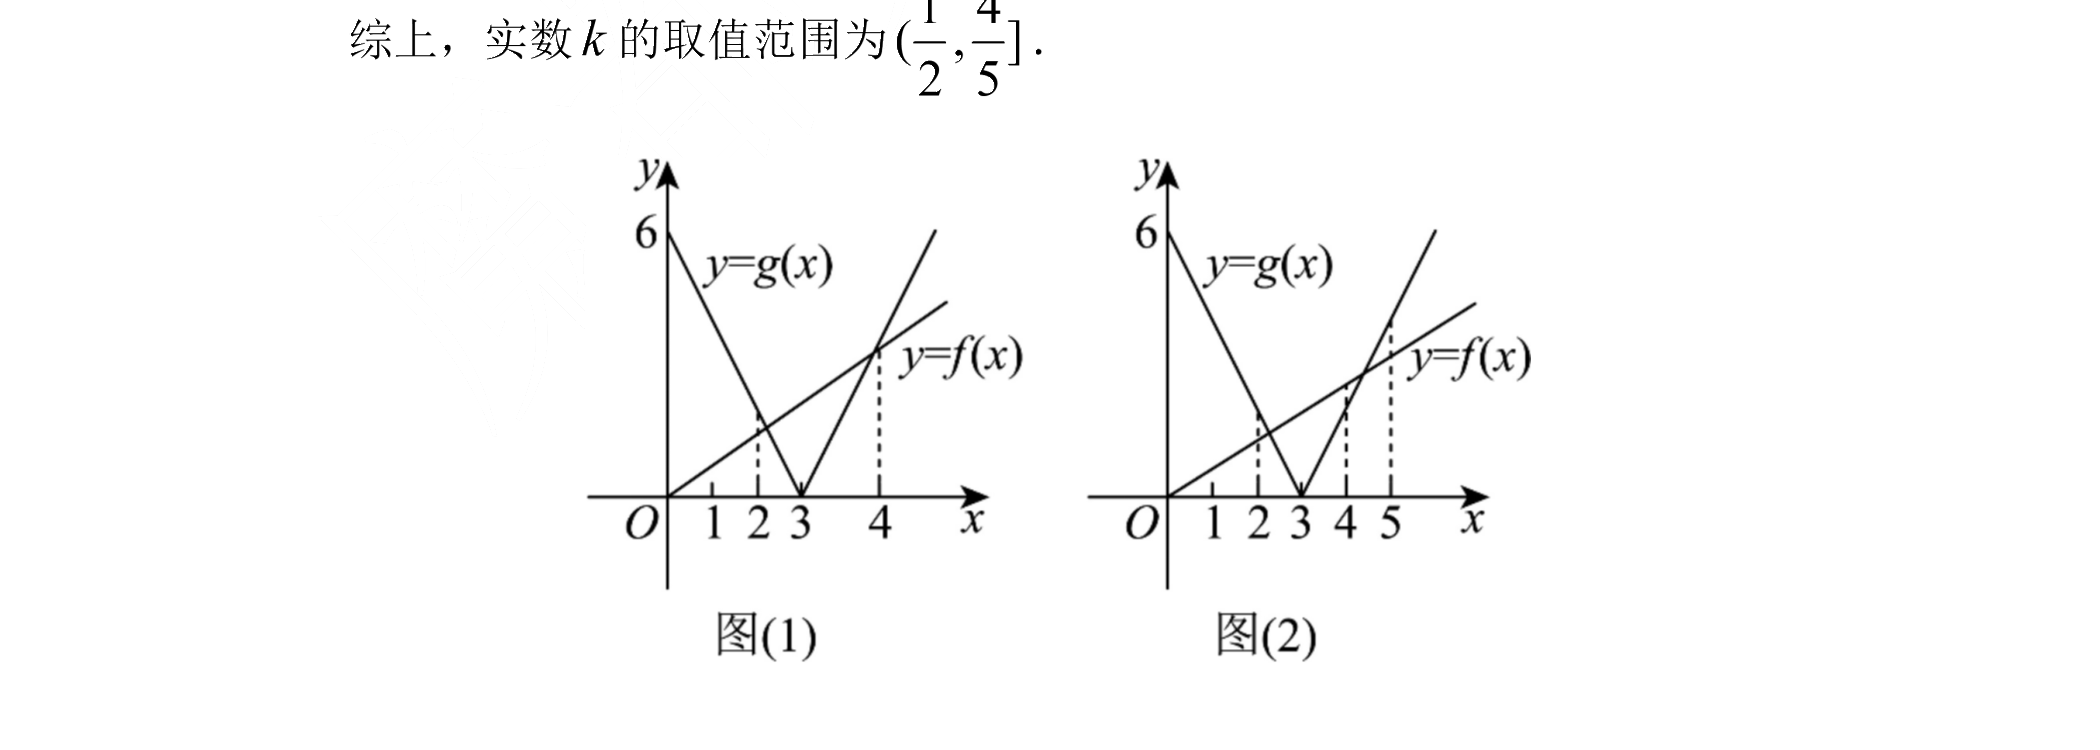
\includegraphics[width=0.72\textwidth]{figures/gao108_q11.png}
\end{center}

\step{综上，实数 $k$ 的取值范围为 $\left(\dfrac12,\dfrac45\right]$.}
\solend
\fi

\item 已知集合 $A=[1,a]\cup[a^3,a^4]$，集合 $B=\{x\mid x=x_1-x_2$，其中 $x_1$,$x_2\in A\}$. 若集合 $B$ 表
示的区间为一个闭区间，则实数 $a$ 的取值范围为\blankline[4.4em].

\ifanswer
\solbegin
\step{由题意得 $a^3>a>1$，则 $x_1-x_2$ 的最小值为 $1-a^4$，最大值为 $a^4-1$,}
\step{所以 $B=[1-a^4,a^4-1]$,}
\step{又因为 $a^4-a^3-(a-1)=a^3(a-1)-(a-1)=(a^3-1)(a-1)>0$,}
\step{所以 $a^4-a^3>a-1$，又集合 $B$ 表示的区间为一个闭区间,}
\step{则 $a^3-a\leqslant a^4-a^3$，化简得 $a^2-a-1\geqslant0$，又 $a>1$，解得 $a\geqslant\dfrac{1+\sqrt5}2$.}
\solend
\fi

\end{enumerate}

\bigsec{二、选择题}

\begin{enumerate}
\setcounter{enumi}{12}

\item 若 $a,b,c\in\R$，则下列不等式恒成立的是\mbox{（\quad）}% 原卷把答案“C”印在题干括号内、无【解析】

\keepwithprev
A. $\dfrac1a<\dfrac1b$\qquad B. $a^2<b^2$\qquad C. $\dfrac{a}{c^2+1}>\dfrac{b}{c^2+1}$\qquad D. $a\lvert c\rvert>b\lvert c\rvert$

\ifanswer
\ans{$C$}
\fi

\item 以下几个关系中正确的是\mbox{（\quad）}

\keepwithprev
A. $0\in\varnothing$\qquad\qquad\qquad B. $\varnothing\in\{x\mid x^2+1=0\}$

C. $\varnothing\subset\{0\}$\qquad\qquad\qquad D. $(A\cap B)\subset(A\cup B)$

\ifanswer
\solbegin
\step{$A$ 选项，$\varnothing$ 不包含任何元素，所以 $0\in\varnothing$ 错误，$A$ 错,}
\step{$B$ 选项，集合与集合之间关系不可以用 $\in$，$B$ 错,}
\step{$C$ 选项，空集是非空集合的真子集，所以 $\varnothing\subset\{0\}$ 正确，$C$ 对,}
\step{$D$ 选项，当 $A=B$ 时，$(A\cap B)=(A\cup B)$，$D$ 错,}
\step{故选 $C$.}
\solend
\fi

\item 设全集为 $U$，图中阴影部分所表示的集合是\mbox{（\quad）}% 原卷把答案“A”印在题干括号内、无【解析】

\keepwithprev
A. $B\cap\overline{A\cup C}$\qquad\qquad B. $(A\cup B)\cap(B\cup C)$

C. $(A\cup C)\cap\overline B$\qquad\qquad D. $(\overline A\cup\overline C)\cap B$

\ifanswer
\ans{$A$}
\fi

\item 对于 $k=0,1,2,\cdots$，定义集合 $A_k=\{20+k,26+2k\}$，并记 $S_k=A_0\cup A_1\cup\cdots\cup A_k$，则
使得集合 $S_n$ 中完全平方数的个数为奇数的最小正整数 $n$ 为\mbox{（\quad）}

\keepwithprev
A. $18$\qquad\qquad B. $19$\qquad\qquad C. $20$\qquad\qquad D. $21$

\ifanswer
\solbegin
\step{当 $k=0$ 时，$A_0=\{20,26\}$，对于 $k=0,1,2,\cdots$,}
\step{集合 $A_k$ 中最小的元素 $20>4^2$，若 $S_n$ 中完全平方数的个数为奇数，则 $n>4$,}
\step{（1）$20+k=5^2$ 时，$k=5$，$A_5=\{25,36\}$，此时 $S_5$ 中完全平方数为 $5^2$、$6^2$,}
\step{个数为 2;}
\step{$20+k=6^2$ 时，$k=16$，$A_{16}=\{36,58\}$，此时 $S_{16}$ 中完全平方数为 $5^2$、$6^2$,}
\step{个数为 2;}
\step{$20+k=7^2$ 时，$k=29$，$A_{29}=\{49,84\}$,}
\step{此时 $S_{29}$ 中完全平方数为 $5^2$、$6^2$、$7^2$、$8^2$，个数为 4;}
\step{$20+k=8^2$ 时，$k=44$，$A_{44}=\{64,114\}$,}
\step{此时 $S_{44}$ 中完全平方数为 $5^2$、$6^2$、$7^2$、$8^2$、$10^2$，个数为 5;}
\step{（2）因为 $k=0,1,2,\cdots,26+2k$ 一定为偶数,}
\step{所以 $26+2k=6^2$ 时，$k=5$，由上述分析得 $S_5$ 中完全平方数个数为 2;}
\step{$26+2k=8^2$ 时，$k=19$，$A_{19}=\{39,64\}$,}
\step{此时 $S_{19}$ 中完全平方数为 $5^2$、$6^2$、$8^2$，个数为 3.}
\step{综上，使集合 $S_n$ 中完全平方数的个数为奇数的最小正整数 $n=19$. 故选 $B$.}
\solend
\fi

\end{enumerate}

\bigsec{三、解答题}

\begin{enumerate}
\setcounter{enumi}{16}

\item 设全集 $U=\R$，集合 $A=\left\{x\,\middle|\,\dfrac{x-2}{x+2}\leqslant0\right\}$，$B=\{x\mid a\leqslant x<2a+1,a\in\R\}$，
$C=\{x\mid\lvert2x-1\rvert<5\}$.

（1）求集合 $A$、$\overline A\cup C$；

（2）若 $B\subseteq A$，求实数 $a$ 的取值范围.

\ifanswer
\solbegin
\ansspace*
\step{（1）不等式 $\dfrac{x-2}{x+2}\leqslant0$，等价于
$\begin{cases}(x-2)(x+2)\leqslant0\\x+2\neq0\end{cases}$，
解得 $\{x\mid-2<x\leqslant2\}$,}
\step{所以 $A=\{x\mid-2<x\leqslant2\}$，则 $\overline A=\{x\mid x\leqslant-2$ 或 $x>2\}$,}
\step{因为 $C=\{x\mid\lvert2x-1\rvert<5\}=\{x\mid-2<x<3\}$，所以 $\overline A\cup C=\R$；}
\step{（2）因为 $B\subseteq A$,}
\step{若 $B=\varnothing$，则 $a\geqslant2a+1$，解得 $a\leqslant-1$,}
\step{若 $B\neq\varnothing$，则
$\begin{cases}a<2a+1\\a>-2\\2a+1\leqslant2\end{cases}$，
解得 $-1<a\leqslant\dfrac12$,}
\step{综上所述，实数 $a$ 的取值范围为 $\left\{a\,\middle|\,a\leqslant\dfrac12\right\}$.}
\solend
\fi

\item 设 $a$、$b$、$c$、$d$ 是四个正数.

（1）已知 $a>b$，比较 $\dfrac{2a+b}{a+2b}$ 与 $\dfrac ab$ 的值的大小；

（2）若 $(1+a)(1+b)(1+c)(1+d)<16$，求证：$a$、$b$、$c$、$d$ 中至少有一个小于 1.

\ifanswer
\solbegin
\step{（1）$\dfrac{2a+b}{a+2b}-\dfrac ab=\dfrac{b^2-a^2}{b(a+2b)}<0$，所以 $\dfrac{2a+b}{a+2b}<\dfrac ab$.}
\step{（2）假设 $a$、$b$、$c$、$d$ 都不小于 1，即 $a$、$b$、$c$、$d$ 均大于等于 1,}
\step{即 $a\geqslant1$，$b\geqslant1$，$c\geqslant1$，$d\geqslant1$,}
\step{由均值不等式得 $1+a\geqslant2\sqrt a$,$1+b\geqslant2\sqrt b$,$1+c\geqslant2\sqrt c$,$1+d\geqslant2\sqrt d$,}
\step{故 $(1+a)(1+b)(1+c)(1+d)\geqslant16\sqrt{abcd}\geqslant16$,}
\step{当且仅当 $a=b=c=d=1$ 时取等号,}
\step{这与 $(1+a)(1+b)(1+c)(1+d)<16$ 矛盾，故假设不成立，原命题成立.}
\solend
\fi

\item 已知 $m\in\R$，一个二次项系数为 1 的一元二次方程的两个不等实根分别为 $x_1$ 和 $x_2$，且
满足
$\begin{cases}x_1^2+x_2^2=2m^2-4\\x_1+x_2=m\end{cases}$.

（1）直接写出该一元二次方程；

（2）若 $(3x_1-x_2)(3x_2-x_1)\geqslant-1$，求 $m$ 的取值范围；

（3）若方程的两根 $x_1$ 和 $x_2$ 都大于 $-1$，求 $m$ 的取值范围.

\ifanswer
\solbegin
\step{（1）设这个一元二次方程为 $x^2+bx+c=0$,}
\step{由
$\begin{cases}x_1^2+x_2^2=2m^2-4\\x_1+x_2=m\end{cases}$,}
\step{得 $(x_1+x_2)^2=x_1^2+x_2^2+2x_1x_2=2m^2-4+2x_1x_2=m^2$，即 $x_1x_2=\dfrac{4-m^2}2$,}
\step{由韦达定理得 $x_1+x_2=-b=m$，即 $x_1x_2=c=\dfrac{4-m^2}2$,}
\step{所以一元二次方程为 $x^2-mx+\dfrac{4-m^2}2=0$.}
\step{（2）$(3x_1-x_2)(3x_2-x_1)=9x_1x_2-3x_1^2-3x_2^2+x_1x_2=10x_1x_2-3(x_1^2+x_2^2)\geqslant-1$,}
\step{结合已知及（1）得 $x_1^2+x_2^2=2m^2-4$,$x_1x_2=\dfrac{4-m^2}2$,}
\step{代入得 $10\times\dfrac{4-m^2}2-3(2m^2-4)=-11m^2+32\geqslant-1\Rightarrow m^2\leqslant3$}
\step{$\Rightarrow-\sqrt3\leqslant m\leqslant\sqrt3$,}
\step{又 $\Delta=m^2-4\times\dfrac{4-m^2}2=3m^2-8>0\Rightarrow m<-\dfrac{2\sqrt6}3$ 或 $m>\dfrac{2\sqrt6}3$,}
\step{所以 $m\in\left[-\sqrt3,-\dfrac{2\sqrt6}3\right)\cup\left(\dfrac{2\sqrt6}3,\sqrt3\right]$.}
\step{（3）若方程的两根 $x_1$ 和 $x_2$ 都大于 $-1$，则
$\begin{cases}\Delta>0\\x_1+x_2>-2\\(x_1+1)(x_2+1)>0\end{cases}$,}
\step{所以
$\begin{cases}\Delta=3m^2-8>0\\m>-2\\[2pt]\dfrac{4-m^2}2+m+1>0\end{cases}$，
解得 $m\in\left(1-\sqrt7,-\dfrac{2\sqrt6}3\right)\cup\left(\dfrac{2\sqrt6}3,1+\sqrt7\right)$.}
\solend
\fi

\item 已知不等式 $2\leqslant ax^2+bx+c\leqslant3$ 的解集为 $\{x\mid2\leqslant x\leqslant3\}$.

（1）若 $a>0$，求 $6b+5c$ 的值；

（2）若 $a>0$，且不等式 $ax^2+(b-3)x-c\leqslant0$ 有且仅有 9 个整数解，求 $a$ 的取值范围；

（3）若 $a<0$，对任意的 $x<0$，不等式 $(ax-4)(x^2+b+c+1)\geqslant0$ 恒成立，求 $a^2-b+c$
的取值集合.

\ifanswer
\solbegin
\ansspace*
\step{（1）$a>0$,}
\step{结合二次函数图象得不等式 $ax^2+bx+c\leqslant3$ 的解集为 $\{x\mid2\leqslant x\leqslant3\}$,}
\step{且不等式 $ax^2+bx+c\geqslant2$ 的解集为 $R$,}
\step{所以方程 $ax^2+bx+c-3=0$ 的两根分别为 2 和 3,}
\step{则
$\begin{cases}2+3=-\dfrac ba\\[2pt]2\times3=\dfrac{c-3}a\end{cases}$，
得 $b=-5a$，$c=6a+3$,}
\step{所以 $6b+5c=6\times(-5a)+5(6a+3)=15$.}
\step{（2）若 $a>0$，且不等式 $ax^2+(b-3)x-c\leqslant0$ 有且仅有 9 个整数解,}
\step{由（1）得 $b=-5a$，$c=6a+3$,}
\step{不等式 $ax^2+bx+c\geqslant2$ 可化为 $ax^2-5ax+6a+1\geqslant0$.}
\step{由（1）得不等式 $ax^2+bx+c\geqslant2$ 的解集为 $R$,}
\step{所以 $ax^2-5ax+6a+1\geqslant0$ 恒成立,}
\step{所以
$\begin{cases}a>0\\\Delta=25a^2-4a(6a+1)\leqslant0\end{cases}$，
即
$\begin{cases}a>0\\a^2-4a=a(a-4)\leqslant0\end{cases}$，}
\step{解得 $0<a\leqslant4$.}
\step{不等式 $ax^2+(b-3)x-c\leqslant0$ 等价于 $ax^2-(5a+3)x-(6a+3)\leqslant0$,}
\step{所以 $[ax-(6a+3)](x+1)\leqslant0$，得 $-1\leqslant x\leqslant6+\dfrac3a$,}
\step{所以 $7\leqslant6+\dfrac3a<8$，解得 $\dfrac32<a\leqslant3$.}
\step{综上，$a$ 的取值范围为 $\left(\dfrac32,3\right]$.}
\step{（3）因为 $a<0$,}
\step{同（1）分析，不等式 $ax^2+bx+c\geqslant2$ 的解集为 $\{x\mid2\leqslant x\leqslant3\}$,}
\step{$ax^2+bx+c\leqslant3$ 的解集为 $R$,}
\step{所以方程 $ax^2+bx+c-2=0$ 的两根分别为 2 和 3,}
\step{则
$\begin{cases}2+3=-\dfrac ba\\[2pt]2\times3=\dfrac{c-2}a\end{cases}$，
得 $b=-5a$，$c=6a+2$.}
\step{所以不等式 $ax^2+bx+c=ax^2-5ax+6a+2\leqslant3$ 的解集为 $R$,}
\step{则 $ax^2-5ax+6a-1\leqslant0$ 恒成立,}
\step{所以
$\begin{cases}a<0\\\Delta=25a^2-4a(6a-1)\leqslant0\end{cases}$，
即
$\begin{cases}a<0\\a^2+4a=a(a+4)\leqslant0\end{cases}$，}
\step{解得 $-4\leqslant a<0$.}
\step{所以对任意的 $x<0$，不等式 $(ax-4)(x^2+b+c+1)\geqslant0$ 恒成立}
\step{转化为对任意的 $x<0$，不等式 $(ax-4)(x^2+a+3)\geqslant0$ 恒成立.}
\step{方程 $(ax-4)(x^2+a+3)=0$ 的两个根为 $x=\dfrac4a<0$,}
\step{$x=\pm\sqrt{-a-3}$（$a<-3$ 时成立）,}
\step{因而仅当 $ax-4=0$ 与 $x^2+a+3=0$ 的负根重合时满足条件,}
\step{解得唯一解为 $a=-4$，所以 $a^2-b+c=a^2+11a+2=-26$,}
\step{所以 $a^2-b+c$ 的取值集合为 $\{-26\}$.}
\solend
\fi

\item 已知集合 $A=\{1,2,3,4,5,6,7,8\}$，$M=\{(x,y)\mid x\in A,y\in A\}$，从 $M$ 中选取 $n$ 个不同的
元素组成一个序列：$(x_1,y_1)$,$(x_2,y_2),\cdots,(x_n,y_n)$，其中 $(x_i,y_i)$ 称为该序列的第 $i$ 项
（$i=1,2,\cdots,n$），若该序列的相邻项 $(x_i,y_i)$,$(x_{i+1},y_{i+1})$ 满足：
\[\begin{cases}\lvert x_{i+1}-x_i\rvert=3\\\lvert y_{i+1}-y_i\rvert=4\end{cases}
\quad\text{或}\quad
\begin{cases}\lvert x_{i+1}-x_i\rvert=4\\\lvert y_{i+1}-y_i\rvert=3\end{cases}\]
（$i=1,2,\cdots,n-1$），则称该序列为“$\Delta-$序列”.

（1）若一个 $\Delta-$序列的第一项为 $(4,4)$，请直接写出它所有可能的第二项；

（2）定义集合 $A=\{1,2,3,4,5,6,7,8\}$ 的两个子集：外侧集 $S=\{1,2,7,8\}$，内侧集
$T=\{3,4,5,6\}$. 证明：若 $\Delta-$序列中某一项的坐标在区域 $S\times S$ 内（即横、纵坐标均属于
$S$），则它的下一项坐标必定在区域 $T\times T$ 内；

（3）证明：不存在一个恰好有 5 项的 $\Delta-$序列，使其第一项为 $(1,8)$，且第五项为
$(8,1)$.

\ifanswer
\solbegin
\ansspace*
\step{（1）由题意，第一项为 $(x_1,y_1)=(4,4)$,}
\step{对于第二项 $(x_2,y_2)$，其坐标必须在 1~8 之间.}
\step{若 $\lvert x_2-4\rvert=3$,$\lvert y_2-4\rvert=4$，则 $x_2\in\{1,7\}$,}
\step{且 $y_2\in\{8\}$（因为 $4-4=0$ 不在集合 $A$ 中）. 此时可能的点为 $(1,8)$,$(7,8)$.}
\step{若 $\lvert x_2-4\rvert=4$,$\lvert y_2-4\rvert=3$，则 $x_2\in\{8\}$，且 $y_2\in\{1,7\}$.}
\step{此时可能的点为 $(8,1)$,$(8,7)$.}
\step{所以它所有可能的第二项为 $(1,8)$,$(7,8)$,$(8,1)$,$(8,7)$.}
\step{（2）已知某一项 $(x_t,y_t)\in S\times S$，即 $x_t\in\{1,2,7,8\}$ 且 $y_t\in\{1,2,7,8\}$.}
\step{由规则得下一步坐标的变化量为 3 和 4，设 $a\in S$ 变化 3 或 4 后的结果 $a'$:}
\step{当 $a=1$ 时，$1+3=4\in T$,$1+4=5\in T$；}
\step{当 $a=2$ 时，$2+3=5\in T$,$2+4=6\in T$；}
\step{当 $a=7$ 时，$7-3=4\in T$,$7-4=3\in T$；}
\step{当 $a=8$ 时，$8-3=5\in T$,$8-4=4\in T$.}
\step{（注：由于超出 1~8 范围的越界坐标不符合.）}
\step{由此可见，无论 $a$ 是 $S$ 中的哪一个数，加上或减去 3 或 4 之后,}
\step{得到的新坐标必属于集合 $T$.}
\step{因为 $\Delta-$序列每走一步，横坐标和纵坐标必定同时发生 3 和 4 的变化,}
\step{所以新的横坐标 $x_{i+1}$ 必属于 $T$，新的纵坐标 $y_{i+1}$ 也必属于 $T$,}
\step{即下一项 $(x_{i+1},y_{i+1})$ 必定在区域 $T\times T$ 内. ………10 分原命题得证.% 得分行混入证明，照录
}
\step{（3）假设存在这样一个包含 5 项的 $\Delta-$序列:}
\step{$(x_1,y_1)$,$(x_2,y_2)$,$(x_3,y_3)$,$(x_4,y_4)$,$(x_5,y_5)$.}
\step{已知第一项为 $(1,8)$，第五项为 $(8,1)$. 第 2 项必须是第 1 项 $(1,8)$ 的相邻点.}
\step{我们来找 $(1,8)$ 的相邻点：第 2 项只能是 $(4,4)$ 或 $(5,5)$,}
\step{第 4 项必须是第 5 项 $(8,1)$ 的相邻点（因为跳跃是双向可逆的）.}
\step{同理可算得，$(8,1)$ 的相邻点也只有两个：$(4,4)$ 和 $(5,5)$,}
\step{题目题干中明确规定，$\Delta-$序列由 $n$ 个不同的有序数对构成.% “题目题干”措辞重复，照录
}
\step{所以，第 2 项和第 4 项不能是同一个点. 这就意味着:}
\step{如果第 2 项是 $(4,4)$，第 4 项就必须是 $(5,5)$；反之亦然.}
\step{则第 3 项必须是 $(4,4)$ 和 $(5,5)$ 的公共相邻点.}
\step{$(4,4)$ 的相邻点集合为：$\{(1,8),(7,8),(8,1),(8,7)\}$,}
\step{$(5,5)$ 的相邻点集合为：$\{(2,1),(8,1),(1,2),(1,8)\}$,}
\step{所以，第 3 项只能填 $(1,8)$ 或者 $(8,1)$.}
\step{这与“序列由不同的有序数对构成”这一条件产生矛盾！}
\step{所以，不存在一个恰好有 5 项的 $\Delta-$序列,}
\step{使其第一项为 $(1,8)$，且第五项为 $(8,1)$.}
\solend
\fi

\end{enumerate}

\end{document}
"
%
% 原始材料：微信公众号“魔都数学加油站”文章，作者破晓，2026-11-03 17:19 发布；
% 连载“27学年高一108”，原文标题“27学年高一108——2026-2027年上海市五校联考高一上10月月考”；
% 原文链接：https://mp.weixin.qq.com/s/3nkP789Qar93NGMZXFFCSw。
% 正文为 14 张 PNG 页（第 2、3、6—13 页 4762×6735，第 1、4、5、14 页 2560×3620），
% 题目下印有【解析】，为讲评版。
% 题目、解析均据原图转录；卷面水印及公众号页脚未录入。
% 第 6 题解析的文氏图与第 11 题法二解析的两幅图象（图(1)、图(2)）裁自原图、去粉色水印
% 转灰度（gao108_q6.png、gao108_q11.png），第 6 题图属解析（仅答案版）、
% 第 11 题图属解析（仅答案版）。
%
% 卷首标题：原卷印作“2026-2027 年五校联考高一上 10 月月考”，标题下另印一行参与学校
% 名单“闵行中学、嘉定一中、松江一中、金山中学、嘉一实高”（全稿第 5 份原卷自印副标题，
% 按 14／24／49／50 成例照录，并登记进计数核对.py 的 SELFSUB）。
%
% 与原卷的排版差异：
%   ① 原文从第 3 题起，填空题编号为 3—12、选择题为 13—16、解答题为 17—21，本稿保留原题号；
%   ② 原卷每题下直接印【解析】，本稿按全稿惯例将解析置于答案版；第 4 题只印【答案】，
%      第 13、15 两题把答案印在题干括号内且无【解析】，均另提 \ans{}；
%   ③ 原卷副标题照录（见上）；
%   ④ 原卷填空横线按全稿惯例排为 \blankline[4.4em]；解答题按惯例加 \ansspace；选择题括号排
%      \mbox{（\quad）}、选项段前按惯例加 \keepwithprev；
%   ⑤ 原卷数集排斜体 $R$／$N$，按全稿惯例改 \R、\N。
%
% 原卷红色强调照录为黑体：第 11 题解析的“法一：”“法二：”原卷排红色，按 53 成例排
% \stepm{法一：}／\stepm{法二：}（加粗着色）。
%
% 原卷存疑：第 10 题题干“变项和”定义中“将 $M$ 中每个元素 $m$ 都乘以 $(-1)^n$ 后再求和”
% 的 $n$ 未加界定（据解析应为该元素在 $\{1,2,\cdots,2026\}$ 中的序号），照录。
% 第 21 题 (2) 解析末行“即下一项 $(x_{i+1},y_{i+1})$ 必定在区域 $T\times T$ 内. ………10 分
% 原命题得证.”，原卷把得分点行混入证明（“原命题”按上下文为“原命题的逆否”），照录。
% 第 21 题 (3) 解析“题目题干中明确规定”，“题目题干”措辞重复，照录。
%
% 行数核对：逐题数 \step/\stepm 条数，合计 164 条（Q3：3；Q4：0；Q5：2；Q6：1；Q7：3；
% Q8：3；Q9：3；Q10：6；Q11：21；Q12：5；Q13：0；Q14：5；Q15：0；Q16：15；Q17：7；
% Q18：7；Q19：13；Q20：34；Q21：36），与原卷印刷行逐题相等。第 4 题只印【答案】、
% 第 13、15 题括号内印答案，均提 \ans{}，不计入 \step 账。
%
\documentclass[a4paper,11pt]{article}
\usepackage{common}

\begin{document}

\examtitlest[3]{2026--2027 年五校联考高一上 10 月月考}{闵行中学、嘉定一中、松江一中、金山中学、嘉一实高}

\bigsec{一、填空题}

\begin{enumerate}
\setcounter{enumi}{2}

\item 已知等式 $2x^2+3x+5=2ax^2+a(3x+1)+c$ 恒成立，则实数 $a+c$ 的值为\blankline[4.4em].

\ifanswer
\solbegin
\step{因为 $2x^2+3x+5=2ax^2+a(3x+1)+c$ 恒成立,}
\step{即 $2x^2+3x+5=2ax^2+3ax+(a+c)$ 恒成立，所以
$\begin{cases}2=2a\\3=3a\\5=a+c\end{cases}$,}
\step{所以 $a+c=5$.}
\solend
\fi

\item 不等式 $\dfrac1x<\dfrac12$ 的解集是\blankline[4.4em].

\ifanswer
\ans{$(-\infty,0)\cup(2,+\infty)$}
\fi

\item 已知 $a$、$b$ 都是实数，则“$a^2=b^2$”是“$a^2+b^2=2ab$”的\blankline[4.4em]条件.

\ifanswer
\solbegin
\step{$a^2=b^2$ 等价于 $a=\pm b$；$a^2+b^2=2ab$ 等价于 $(a-b)^2=0$ 等价于 $a=b$,}
\step{故“$a^2=b^2$”是“$a^2+b^2=2ab$”的必要不充分条件.}
\solend
\fi

\item 已知全集 $U=\{x\mid x$ 为不大于 20 的素数$\}$，$A\cap\overline B=\{5\}$，$\overline A\cap B=\{3\}$，
$\overline{A\cup B}=\{7,13,17,19\}$，则 $A=$\blankline[4.4em].

\ifanswer
\solbegin
\step{如图所示，$A=\{2,5,11\}$.}

\begin{center}
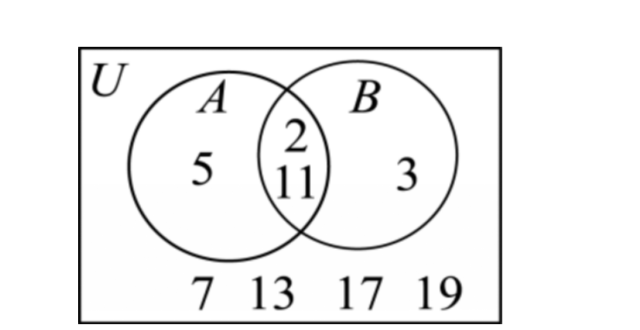
\includegraphics[width=0.24\textwidth]{figures/gao108_q6.png}
\end{center}

\solend
\fi

\item 若 $x\in A$，则 $\dfrac1x\in A$，就称 $A$ 自倒集合，集合 $M=\left\{-2,-1,0,\dfrac12,\dfrac13,1,2,3,4\right\}$ 的所有非空
子集中，自倒集合的个数为\blankline[4.4em].

\ifanswer
\solbegin
\step{由新定义，集合 $M$ 中的元素 1 和 $-1$ 倒数等于本身，2 和 $\dfrac12$，3 和 $\dfrac13$ 互为倒数,}
\step{故满足条件的自倒集合与集合 $\{-1,1,2,3\}$ 的非空子集的个数相同,}
\step{则其个数为 $2^4-1=15$.}
\solend
\fi

\item 设集合 $M=\{(x,y)\mid y=x^2+2bx+1\}$，$N=\{(x,y)\mid y=x+b\}(b\in\R)$，若
$M\cap N=\varnothing$，则实数 $b$ 的取值范围为\blankline[4.4em].

\ifanswer
\solbegin
\step{因为 $M\cap N=\varnothing$，所以
$\begin{cases}y=x^2+2bx+1\\y=x+b\end{cases}$
无解，则 $x^2+(2b-1)x+(1-b)=0$,}
\step{则 $\triangle=(2b-1)^2-4\times1\times(1-b)=4b^2-3<0$，解得 $-\dfrac{\sqrt3}2<b<\dfrac{\sqrt3}2$,}
\step{即实数 $b$ 的取值范围为 $\left(-\dfrac{\sqrt3}2,\dfrac{\sqrt3}2\right)$.}
\solend
\fi

\item 已知集合 $A=\left\{x\,\middle|\,\dfrac{x-a}{x^2-1}=1\right\}$ 有唯一元素，用列举法表示满足集合 $A$ 的条件的 $a$ 的取值集
合\blankline[4.4em].

\ifanswer
\solbegin
\step{$a=1$,$\dfrac{1}{x+1}=1$，一解；$a=-1$,$\dfrac{1}{x-1}=1$，一解；}
\step{$x-a=x^2-1$，一解时，$a=\dfrac54$,}
\step{综上，$a$ 的取值集合为 $\left\{-1,1,\dfrac54\right\}$.}
\solend
\fi

\item 已知集合 $M$ 的元素均为正整数，定义集合 $M$ 的“变项和”为：将 $M$ 中每个元素 $m$ 都乘
以 $(-1)^n$ 后再求和. 若集合 $A=\{n\mid1\leqslant n\leqslant2026,n\in\N\}$，则集合 $A$ 的所有非空子集的“变
项和”的总和为\blankline[4.4em].% $n$ 未加界定（据解析为元素序号），照录

\ifanswer
\solbegin
\step{$A=\{n\mid1\leqslant n\leqslant2026,n\in\N\}=\{1,2,\cdots,2026\}$,}
\step{1 在所有非空子集中共出现 $C_{2025}^{0}+C_{2025}^{1}+\cdots+C_{2025}^{2025}=2^{2025}$ 次,}
\step{同理 $2,3,\cdots,2026$ 都出现 $2^{2025}$ 次,}
\step{则集合 $A$ 的所有非空子集的“变项和”的总和}
\step{为 $2^{2025}\times[1\times(-1)^1+2\times(-1)^2+\cdots+2026\times(-1)^{2026}]$}
\step{$=2^{2025}\times(-1+2-3+4-\cdots-2025+2026)=1013\times2^{2025}$.}
\solend
\fi

\item 已知 $0<k<2$，定义 $[x]$ 为不超过 $x$ 的最大整数，区间 $[a,b]$（或 $(a,b)$，$[a,b)$，
$(a,b]$）的长度记为 $b-a$. 若关于 $x$ 的不等式 $k[x]>\lvert2[x]-6\rvert$ 的解集对应区间的长度为 $2$，
则 $k$ 的取值范围是\blankline[4.4em].

\ifanswer
\solbegin
\stepm{法一：}{由题意得 $\lvert2[x]-6\rvert=
\begin{cases}2[x]-6,x\geqslant3\\-2[x]+6,x<3\end{cases}$.}
\step{①当 $x\geqslant3$ 时，不等式 $k[x]>\lvert2[x]-6\rvert$ 可化为 $k[x]>2[x]-6$,}
\step{即 $(2-k)[x]<6$,}
\step{当 $0<k<2$ 时，解不等式 $(2-k)[x]<6$ 得 $[x]<\dfrac6{2-k}$.}
\step{②当 $x<3$ 时，不等式 $k[x]>\lvert2[x]-6\rvert$ 可化为 $k[x]>-2[x]+6$,}
\step{即 $(k+2)[x]>6$.}
\step{当 $0<k<2$ 时，解不等式 $(k+2)[x]>6$ 得 $[x]>\dfrac6{k+2}$.}
\step{综上所述，不等式 $k[x]>\lvert2[x]-6\rvert$ 的解集需满足 $\dfrac6{k+2}<[x]<\dfrac6{2-k}$,}
\step{由题意得在区间 $\left[\dfrac6{k+2},\dfrac6{2-k}\right]$ 内有两个整数,}
\step{由于 $\dfrac6{k+2}\in\left(\dfrac32,3\right)$，所以 $\dfrac6{2-k}\leqslant5$，得 $k\leqslant\dfrac45$.}
\step{因此 $k\in\left(0,\dfrac45\right]$，得 $\dfrac6{k+2}\in\left[\dfrac75,3\right)$，$\dfrac6{2-k}\in(3,5]$,}
\step{区间 $\left[\dfrac6{k+2},\dfrac6{2-k}\right]$ 内的两个整数是 3、4，所以 $4<\dfrac6{2-k}\leqslant5$，解得 $\dfrac12<k\leqslant\dfrac45$,}
\step{即 $k\in\left(\dfrac12,\dfrac45\right]$.}
\stepm{法二：}{令 $f(x)=kx$，$g(x)=\lvert2x-6\rvert$，画出 $g(x)$、$f(x)$ 的图象,}
\step{由于不等式 $k[x]>\lvert2[x]-6\rvert$ 的解集对应区间的长度为 2,}
\step{因此解集只可能为 $[3,5)$ 或 $[2,4)$.}
\step{当解集为 $[3,5)$ 时，如图（2），数形结合易得
$\begin{cases}f(2)\leqslant g(2)\\f(4)>g(4)\\f(5)\leqslant g(5)\end{cases}$,}
\step{即
$\begin{cases}2k\leqslant\lvert2\times2-6\rvert\\4k>\lvert2\times4-6\rvert\\5k\leqslant\lvert2\times5-6\rvert\end{cases}$，
解得
$\begin{cases}k\leqslant1\\k>\dfrac12\\k\leqslant\dfrac45\end{cases}$，
所以 $\dfrac12<k\leqslant\dfrac45$，满足 $0<k<2$,}
\step{当解集为 $[2,4)$ 时，如图（1），数形结合易得
$\begin{cases}f(2)>g(2)\\f(4)\leqslant g(4)\end{cases}$,}
\step{即
$\begin{cases}2k>\lvert2\times2-6\rvert\\4k\leqslant\lvert2\times4-6\rvert\end{cases}$，
无解.}

\begin{center}
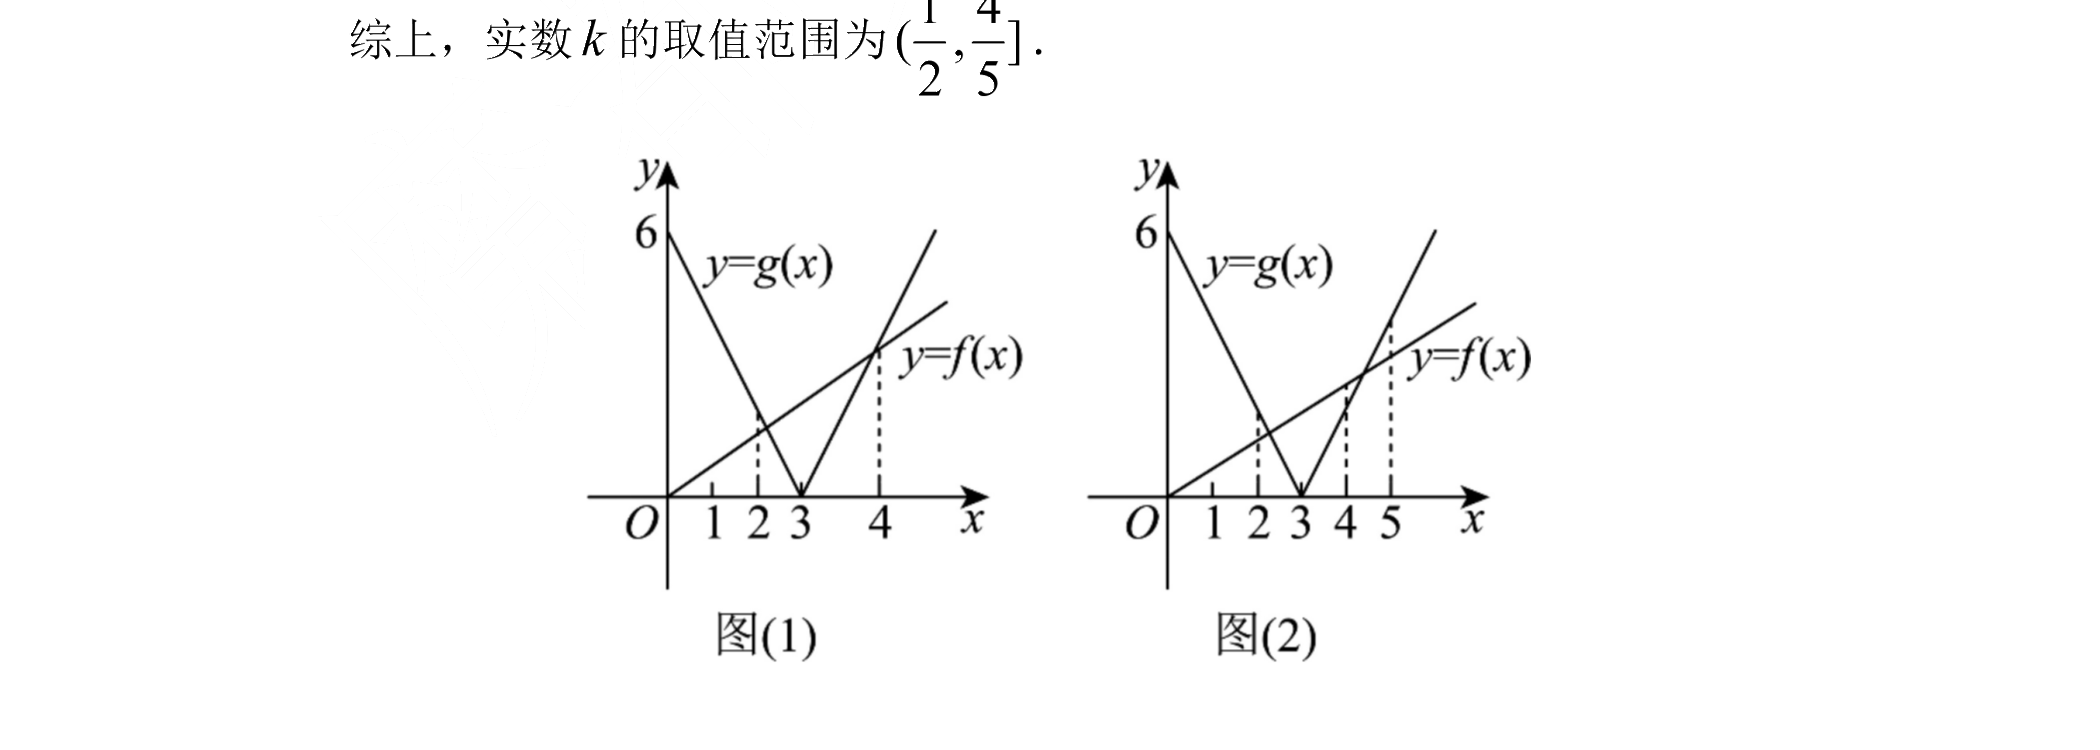
\includegraphics[width=0.72\textwidth]{figures/gao108_q11.png}
\end{center}

\step{综上，实数 $k$ 的取值范围为 $\left(\dfrac12,\dfrac45\right]$.}
\solend
\fi

\item 已知集合 $A=[1,a]\cup[a^3,a^4]$，集合 $B=\{x\mid x=x_1-x_2$，其中 $x_1$,$x_2\in A\}$. 若集合 $B$ 表
示的区间为一个闭区间，则实数 $a$ 的取值范围为\blankline[4.4em].

\ifanswer
\solbegin
\step{由题意得 $a^3>a>1$，则 $x_1-x_2$ 的最小值为 $1-a^4$，最大值为 $a^4-1$,}
\step{所以 $B=[1-a^4,a^4-1]$,}
\step{又因为 $a^4-a^3-(a-1)=a^3(a-1)-(a-1)=(a^3-1)(a-1)>0$,}
\step{所以 $a^4-a^3>a-1$，又集合 $B$ 表示的区间为一个闭区间,}
\step{则 $a^3-a\leqslant a^4-a^3$，化简得 $a^2-a-1\geqslant0$，又 $a>1$，解得 $a\geqslant\dfrac{1+\sqrt5}2$.}
\solend
\fi

\end{enumerate}

\bigsec{二、选择题}

\begin{enumerate}
\setcounter{enumi}{12}

\item 若 $a,b,c\in\R$，则下列不等式恒成立的是\mbox{（\quad）}% 原卷把答案“C”印在题干括号内、无【解析】

\keepwithprev
A. $\dfrac1a<\dfrac1b$\qquad B. $a^2<b^2$\qquad C. $\dfrac{a}{c^2+1}>\dfrac{b}{c^2+1}$\qquad D. $a\lvert c\rvert>b\lvert c\rvert$

\ifanswer
\ans{$C$}
\fi

\item 以下几个关系中正确的是\mbox{（\quad）}

\keepwithprev
A. $0\in\varnothing$\qquad\qquad\qquad B. $\varnothing\in\{x\mid x^2+1=0\}$

C. $\varnothing\subset\{0\}$\qquad\qquad\qquad D. $(A\cap B)\subset(A\cup B)$

\ifanswer
\solbegin
\step{$A$ 选项，$\varnothing$ 不包含任何元素，所以 $0\in\varnothing$ 错误，$A$ 错,}
\step{$B$ 选项，集合与集合之间关系不可以用 $\in$，$B$ 错,}
\step{$C$ 选项，空集是非空集合的真子集，所以 $\varnothing\subset\{0\}$ 正确，$C$ 对,}
\step{$D$ 选项，当 $A=B$ 时，$(A\cap B)=(A\cup B)$，$D$ 错,}
\step{故选 $C$.}
\solend
\fi

\item 设全集为 $U$，图中阴影部分所表示的集合是\mbox{（\quad）}% 原卷把答案“A”印在题干括号内、无【解析】

\keepwithprev
A. $B\cap\overline{A\cup C}$\qquad\qquad B. $(A\cup B)\cap(B\cup C)$

C. $(A\cup C)\cap\overline B$\qquad\qquad D. $(\overline A\cup\overline C)\cap B$

\ifanswer
\ans{$A$}
\fi

\item 对于 $k=0,1,2,\cdots$，定义集合 $A_k=\{20+k,26+2k\}$，并记 $S_k=A_0\cup A_1\cup\cdots\cup A_k$，则
使得集合 $S_n$ 中完全平方数的个数为奇数的最小正整数 $n$ 为\mbox{（\quad）}

\keepwithprev
A. $18$\qquad\qquad B. $19$\qquad\qquad C. $20$\qquad\qquad D. $21$

\ifanswer
\solbegin
\step{当 $k=0$ 时，$A_0=\{20,26\}$，对于 $k=0,1,2,\cdots$,}
\step{集合 $A_k$ 中最小的元素 $20>4^2$，若 $S_n$ 中完全平方数的个数为奇数，则 $n>4$,}
\step{（1）$20+k=5^2$ 时，$k=5$，$A_5=\{25,36\}$，此时 $S_5$ 中完全平方数为 $5^2$、$6^2$,}
\step{个数为 2;}
\step{$20+k=6^2$ 时，$k=16$，$A_{16}=\{36,58\}$，此时 $S_{16}$ 中完全平方数为 $5^2$、$6^2$,}
\step{个数为 2;}
\step{$20+k=7^2$ 时，$k=29$，$A_{29}=\{49,84\}$,}
\step{此时 $S_{29}$ 中完全平方数为 $5^2$、$6^2$、$7^2$、$8^2$，个数为 4;}
\step{$20+k=8^2$ 时，$k=44$，$A_{44}=\{64,114\}$,}
\step{此时 $S_{44}$ 中完全平方数为 $5^2$、$6^2$、$7^2$、$8^2$、$10^2$，个数为 5;}
\step{（2）因为 $k=0,1,2,\cdots,26+2k$ 一定为偶数,}
\step{所以 $26+2k=6^2$ 时，$k=5$，由上述分析得 $S_5$ 中完全平方数个数为 2;}
\step{$26+2k=8^2$ 时，$k=19$，$A_{19}=\{39,64\}$,}
\step{此时 $S_{19}$ 中完全平方数为 $5^2$、$6^2$、$8^2$，个数为 3.}
\step{综上，使集合 $S_n$ 中完全平方数的个数为奇数的最小正整数 $n=19$. 故选 $B$.}
\solend
\fi

\end{enumerate}

\bigsec{三、解答题}

\begin{enumerate}
\setcounter{enumi}{16}

\item 设全集 $U=\R$，集合 $A=\left\{x\,\middle|\,\dfrac{x-2}{x+2}\leqslant0\right\}$，$B=\{x\mid a\leqslant x<2a+1,a\in\R\}$，
$C=\{x\mid\lvert2x-1\rvert<5\}$.

（1）求集合 $A$、$\overline A\cup C$；

（2）若 $B\subseteq A$，求实数 $a$ 的取值范围.

\ifanswer
\solbegin
\ansspace*
\step{（1）不等式 $\dfrac{x-2}{x+2}\leqslant0$，等价于
$\begin{cases}(x-2)(x+2)\leqslant0\\x+2\neq0\end{cases}$，
解得 $\{x\mid-2<x\leqslant2\}$,}
\step{所以 $A=\{x\mid-2<x\leqslant2\}$，则 $\overline A=\{x\mid x\leqslant-2$ 或 $x>2\}$,}
\step{因为 $C=\{x\mid\lvert2x-1\rvert<5\}=\{x\mid-2<x<3\}$，所以 $\overline A\cup C=\R$；}
\step{（2）因为 $B\subseteq A$,}
\step{若 $B=\varnothing$，则 $a\geqslant2a+1$，解得 $a\leqslant-1$,}
\step{若 $B\neq\varnothing$，则
$\begin{cases}a<2a+1\\a>-2\\2a+1\leqslant2\end{cases}$，
解得 $-1<a\leqslant\dfrac12$,}
\step{综上所述，实数 $a$ 的取值范围为 $\left\{a\,\middle|\,a\leqslant\dfrac12\right\}$.}
\solend
\fi

\item 设 $a$、$b$、$c$、$d$ 是四个正数.

（1）已知 $a>b$，比较 $\dfrac{2a+b}{a+2b}$ 与 $\dfrac ab$ 的值的大小；

（2）若 $(1+a)(1+b)(1+c)(1+d)<16$，求证：$a$、$b$、$c$、$d$ 中至少有一个小于 1.

\ifanswer
\solbegin
\step{（1）$\dfrac{2a+b}{a+2b}-\dfrac ab=\dfrac{b^2-a^2}{b(a+2b)}<0$，所以 $\dfrac{2a+b}{a+2b}<\dfrac ab$.}
\step{（2）假设 $a$、$b$、$c$、$d$ 都不小于 1，即 $a$、$b$、$c$、$d$ 均大于等于 1,}
\step{即 $a\geqslant1$，$b\geqslant1$，$c\geqslant1$，$d\geqslant1$,}
\step{由均值不等式得 $1+a\geqslant2\sqrt a$,$1+b\geqslant2\sqrt b$,$1+c\geqslant2\sqrt c$,$1+d\geqslant2\sqrt d$,}
\step{故 $(1+a)(1+b)(1+c)(1+d)\geqslant16\sqrt{abcd}\geqslant16$,}
\step{当且仅当 $a=b=c=d=1$ 时取等号,}
\step{这与 $(1+a)(1+b)(1+c)(1+d)<16$ 矛盾，故假设不成立，原命题成立.}
\solend
\fi

\item 已知 $m\in\R$，一个二次项系数为 1 的一元二次方程的两个不等实根分别为 $x_1$ 和 $x_2$，且
满足
$\begin{cases}x_1^2+x_2^2=2m^2-4\\x_1+x_2=m\end{cases}$.

（1）直接写出该一元二次方程；

（2）若 $(3x_1-x_2)(3x_2-x_1)\geqslant-1$，求 $m$ 的取值范围；

（3）若方程的两根 $x_1$ 和 $x_2$ 都大于 $-1$，求 $m$ 的取值范围.

\ifanswer
\solbegin
\step{（1）设这个一元二次方程为 $x^2+bx+c=0$,}
\step{由
$\begin{cases}x_1^2+x_2^2=2m^2-4\\x_1+x_2=m\end{cases}$,}
\step{得 $(x_1+x_2)^2=x_1^2+x_2^2+2x_1x_2=2m^2-4+2x_1x_2=m^2$，即 $x_1x_2=\dfrac{4-m^2}2$,}
\step{由韦达定理得 $x_1+x_2=-b=m$，即 $x_1x_2=c=\dfrac{4-m^2}2$,}
\step{所以一元二次方程为 $x^2-mx+\dfrac{4-m^2}2=0$.}
\step{（2）$(3x_1-x_2)(3x_2-x_1)=9x_1x_2-3x_1^2-3x_2^2+x_1x_2=10x_1x_2-3(x_1^2+x_2^2)\geqslant-1$,}
\step{结合已知及（1）得 $x_1^2+x_2^2=2m^2-4$,$x_1x_2=\dfrac{4-m^2}2$,}
\step{代入得 $10\times\dfrac{4-m^2}2-3(2m^2-4)=-11m^2+32\geqslant-1\Rightarrow m^2\leqslant3$}
\step{$\Rightarrow-\sqrt3\leqslant m\leqslant\sqrt3$,}
\step{又 $\Delta=m^2-4\times\dfrac{4-m^2}2=3m^2-8>0\Rightarrow m<-\dfrac{2\sqrt6}3$ 或 $m>\dfrac{2\sqrt6}3$,}
\step{所以 $m\in\left[-\sqrt3,-\dfrac{2\sqrt6}3\right)\cup\left(\dfrac{2\sqrt6}3,\sqrt3\right]$.}
\step{（3）若方程的两根 $x_1$ 和 $x_2$ 都大于 $-1$，则
$\begin{cases}\Delta>0\\x_1+x_2>-2\\(x_1+1)(x_2+1)>0\end{cases}$,}
\step{所以
$\begin{cases}\Delta=3m^2-8>0\\m>-2\\[2pt]\dfrac{4-m^2}2+m+1>0\end{cases}$，
解得 $m\in\left(1-\sqrt7,-\dfrac{2\sqrt6}3\right)\cup\left(\dfrac{2\sqrt6}3,1+\sqrt7\right)$.}
\solend
\fi

\item 已知不等式 $2\leqslant ax^2+bx+c\leqslant3$ 的解集为 $\{x\mid2\leqslant x\leqslant3\}$.

（1）若 $a>0$，求 $6b+5c$ 的值；

（2）若 $a>0$，且不等式 $ax^2+(b-3)x-c\leqslant0$ 有且仅有 9 个整数解，求 $a$ 的取值范围；

（3）若 $a<0$，对任意的 $x<0$，不等式 $(ax-4)(x^2+b+c+1)\geqslant0$ 恒成立，求 $a^2-b+c$
的取值集合.

\ifanswer
\solbegin
\ansspace*
\step{（1）$a>0$,}
\step{结合二次函数图象得不等式 $ax^2+bx+c\leqslant3$ 的解集为 $\{x\mid2\leqslant x\leqslant3\}$,}
\step{且不等式 $ax^2+bx+c\geqslant2$ 的解集为 $R$,}
\step{所以方程 $ax^2+bx+c-3=0$ 的两根分别为 2 和 3,}
\step{则
$\begin{cases}2+3=-\dfrac ba\\[2pt]2\times3=\dfrac{c-3}a\end{cases}$，
得 $b=-5a$，$c=6a+3$,}
\step{所以 $6b+5c=6\times(-5a)+5(6a+3)=15$.}
\step{（2）若 $a>0$，且不等式 $ax^2+(b-3)x-c\leqslant0$ 有且仅有 9 个整数解,}
\step{由（1）得 $b=-5a$，$c=6a+3$,}
\step{不等式 $ax^2+bx+c\geqslant2$ 可化为 $ax^2-5ax+6a+1\geqslant0$.}
\step{由（1）得不等式 $ax^2+bx+c\geqslant2$ 的解集为 $R$,}
\step{所以 $ax^2-5ax+6a+1\geqslant0$ 恒成立,}
\step{所以
$\begin{cases}a>0\\\Delta=25a^2-4a(6a+1)\leqslant0\end{cases}$，
即
$\begin{cases}a>0\\a^2-4a=a(a-4)\leqslant0\end{cases}$，}
\step{解得 $0<a\leqslant4$.}
\step{不等式 $ax^2+(b-3)x-c\leqslant0$ 等价于 $ax^2-(5a+3)x-(6a+3)\leqslant0$,}
\step{所以 $[ax-(6a+3)](x+1)\leqslant0$，得 $-1\leqslant x\leqslant6+\dfrac3a$,}
\step{所以 $7\leqslant6+\dfrac3a<8$，解得 $\dfrac32<a\leqslant3$.}
\step{综上，$a$ 的取值范围为 $\left(\dfrac32,3\right]$.}
\step{（3）因为 $a<0$,}
\step{同（1）分析，不等式 $ax^2+bx+c\geqslant2$ 的解集为 $\{x\mid2\leqslant x\leqslant3\}$,}
\step{$ax^2+bx+c\leqslant3$ 的解集为 $R$,}
\step{所以方程 $ax^2+bx+c-2=0$ 的两根分别为 2 和 3,}
\step{则
$\begin{cases}2+3=-\dfrac ba\\[2pt]2\times3=\dfrac{c-2}a\end{cases}$，
得 $b=-5a$，$c=6a+2$.}
\step{所以不等式 $ax^2+bx+c=ax^2-5ax+6a+2\leqslant3$ 的解集为 $R$,}
\step{则 $ax^2-5ax+6a-1\leqslant0$ 恒成立,}
\step{所以
$\begin{cases}a<0\\\Delta=25a^2-4a(6a-1)\leqslant0\end{cases}$，
即
$\begin{cases}a<0\\a^2+4a=a(a+4)\leqslant0\end{cases}$，}
\step{解得 $-4\leqslant a<0$.}
\step{所以对任意的 $x<0$，不等式 $(ax-4)(x^2+b+c+1)\geqslant0$ 恒成立}
\step{转化为对任意的 $x<0$，不等式 $(ax-4)(x^2+a+3)\geqslant0$ 恒成立.}
\step{方程 $(ax-4)(x^2+a+3)=0$ 的两个根为 $x=\dfrac4a<0$,}
\step{$x=\pm\sqrt{-a-3}$（$a<-3$ 时成立）,}
\step{因而仅当 $ax-4=0$ 与 $x^2+a+3=0$ 的负根重合时满足条件,}
\step{解得唯一解为 $a=-4$，所以 $a^2-b+c=a^2+11a+2=-26$,}
\step{所以 $a^2-b+c$ 的取值集合为 $\{-26\}$.}
\solend
\fi

\item 已知集合 $A=\{1,2,3,4,5,6,7,8\}$，$M=\{(x,y)\mid x\in A,y\in A\}$，从 $M$ 中选取 $n$ 个不同的
元素组成一个序列：$(x_1,y_1)$,$(x_2,y_2),\cdots,(x_n,y_n)$，其中 $(x_i,y_i)$ 称为该序列的第 $i$ 项
（$i=1,2,\cdots,n$），若该序列的相邻项 $(x_i,y_i)$,$(x_{i+1},y_{i+1})$ 满足：
\[\begin{cases}\lvert x_{i+1}-x_i\rvert=3\\\lvert y_{i+1}-y_i\rvert=4\end{cases}
\quad\text{或}\quad
\begin{cases}\lvert x_{i+1}-x_i\rvert=4\\\lvert y_{i+1}-y_i\rvert=3\end{cases}\]
（$i=1,2,\cdots,n-1$），则称该序列为“$\Delta-$序列”.

（1）若一个 $\Delta-$序列的第一项为 $(4,4)$，请直接写出它所有可能的第二项；

（2）定义集合 $A=\{1,2,3,4,5,6,7,8\}$ 的两个子集：外侧集 $S=\{1,2,7,8\}$，内侧集
$T=\{3,4,5,6\}$. 证明：若 $\Delta-$序列中某一项的坐标在区域 $S\times S$ 内（即横、纵坐标均属于
$S$），则它的下一项坐标必定在区域 $T\times T$ 内；

（3）证明：不存在一个恰好有 5 项的 $\Delta-$序列，使其第一项为 $(1,8)$，且第五项为
$(8,1)$.

\ifanswer
\solbegin
\ansspace*
\step{（1）由题意，第一项为 $(x_1,y_1)=(4,4)$,}
\step{对于第二项 $(x_2,y_2)$，其坐标必须在 1~8 之间.}
\step{若 $\lvert x_2-4\rvert=3$,$\lvert y_2-4\rvert=4$，则 $x_2\in\{1,7\}$,}
\step{且 $y_2\in\{8\}$（因为 $4-4=0$ 不在集合 $A$ 中）. 此时可能的点为 $(1,8)$,$(7,8)$.}
\step{若 $\lvert x_2-4\rvert=4$,$\lvert y_2-4\rvert=3$，则 $x_2\in\{8\}$，且 $y_2\in\{1,7\}$.}
\step{此时可能的点为 $(8,1)$,$(8,7)$.}
\step{所以它所有可能的第二项为 $(1,8)$,$(7,8)$,$(8,1)$,$(8,7)$.}
\step{（2）已知某一项 $(x_t,y_t)\in S\times S$，即 $x_t\in\{1,2,7,8\}$ 且 $y_t\in\{1,2,7,8\}$.}
\step{由规则得下一步坐标的变化量为 3 和 4，设 $a\in S$ 变化 3 或 4 后的结果 $a'$:}
\step{当 $a=1$ 时，$1+3=4\in T$,$1+4=5\in T$；}
\step{当 $a=2$ 时，$2+3=5\in T$,$2+4=6\in T$；}
\step{当 $a=7$ 时，$7-3=4\in T$,$7-4=3\in T$；}
\step{当 $a=8$ 时，$8-3=5\in T$,$8-4=4\in T$.}
\step{（注：由于超出 1~8 范围的越界坐标不符合.）}
\step{由此可见，无论 $a$ 是 $S$ 中的哪一个数，加上或减去 3 或 4 之后,}
\step{得到的新坐标必属于集合 $T$.}
\step{因为 $\Delta-$序列每走一步，横坐标和纵坐标必定同时发生 3 和 4 的变化,}
\step{所以新的横坐标 $x_{i+1}$ 必属于 $T$，新的纵坐标 $y_{i+1}$ 也必属于 $T$,}
\step{即下一项 $(x_{i+1},y_{i+1})$ 必定在区域 $T\times T$ 内. ………10 分原命题得证.% 得分行混入证明，照录
}
\step{（3）假设存在这样一个包含 5 项的 $\Delta-$序列:}
\step{$(x_1,y_1)$,$(x_2,y_2)$,$(x_3,y_3)$,$(x_4,y_4)$,$(x_5,y_5)$.}
\step{已知第一项为 $(1,8)$，第五项为 $(8,1)$. 第 2 项必须是第 1 项 $(1,8)$ 的相邻点.}
\step{我们来找 $(1,8)$ 的相邻点：第 2 项只能是 $(4,4)$ 或 $(5,5)$,}
\step{第 4 项必须是第 5 项 $(8,1)$ 的相邻点（因为跳跃是双向可逆的）.}
\step{同理可算得，$(8,1)$ 的相邻点也只有两个：$(4,4)$ 和 $(5,5)$,}
\step{题目题干中明确规定，$\Delta-$序列由 $n$ 个不同的有序数对构成.% “题目题干”措辞重复，照录
}
\step{所以，第 2 项和第 4 项不能是同一个点. 这就意味着:}
\step{如果第 2 项是 $(4,4)$，第 4 项就必须是 $(5,5)$；反之亦然.}
\step{则第 3 项必须是 $(4,4)$ 和 $(5,5)$ 的公共相邻点.}
\step{$(4,4)$ 的相邻点集合为：$\{(1,8),(7,8),(8,1),(8,7)\}$,}
\step{$(5,5)$ 的相邻点集合为：$\{(2,1),(8,1),(1,2),(1,8)\}$,}
\step{所以，第 3 项只能填 $(1,8)$ 或者 $(8,1)$.}
\step{这与“序列由不同的有序数对构成”这一条件产生矛盾！}
\step{所以，不存在一个恰好有 5 项的 $\Delta-$序列,}
\step{使其第一项为 $(1,8)$，且第五项为 $(8,1)$.}
\solend
\fi

\end{enumerate}

\end{document}
